%\documentclass[12pt,openright]{book}
%\documentclass[12pt,openright,twoside,titlepage,pdf]{LUmanual}
\documentclass[12pt,openright,twoside,titlepage,a4paper]{LUmanual}
\usepackage{ifpdf} 

%\newif\ifpdf
%\ifx\pdfoutput\undefined
%  \pdffalse
%\else
%  \pdftrue
%\fi

%\usepackage[ms]{mccover}
\usepackage{graphicx}
\usepackage{sidecap,caption}
\usepackage{rotating}
\usepackage{multicol,array}
\usepackage[tight,TABTOPCAP]{subfigure}
%\usepackage{times}
%\usepackage{mcfonts}
\usepackage[authoryear]{natbib}
\newcommand\indexname{Indexx}
\usepackage{index}
\usepackage{comment}
\usepackage{url}
%\makeindex
\newindex{xcmds}{cdx}{cnd}{Index of m-files in the tutorial}
\newindex{xentr}{edx}{end}{Index}

\usepackage{latexsym}
\usepackage{supertabular}
\usepackage{xspace}
\usepackage{amsmath,amsfonts}
%\usepackage{tocloft}
%\usepackage[nofancy]{svninfo}
%\usepackage{svninfo}
%\usepackage{showkeys}

\ifpdf
  \pdfoutput=1  % we are running PDFLaTeX
 % \definecolor{blue}{rgb}{0,0,1}
  \usepackage[breaklinks=true,colorlinks,
  citecolor=black,linkcolor=black,
  filecolor=black, menucolor=black,
  urlcolor=black,
  pdftex, 
  pagebackref, backref,
  hyperindex, bookmarks,bookmarksopen]{hyperref}
 \hypersetup{pagebackref,backref,
    pdfauthor = {WAFO-group},
  pdftitle  = {WAFO},
  pdfkeywords={Gaussian processes, non-linear wave, estimation,
    extremes, non-linear simulation, rainflow cycles, fatigue,
    joint distribution, wave height, wave crest
    front velocity, wave crest front steepness, linear and non-linear,
    simulation, wave height,  wave crest velocity,
    ringing, missing observations, outliers, reconstruction,
    multivariate normal probabilities, singular distribution,  wave
    crest amplitude, wave crest velocity,local maxima and minima,
    numerical integration,
    statistical computation, capsize of smaller vessel.}}
  \pdfcompresslevel=9
  \def\pdfBorderAttrs{/Border [0 0 0] }
\else
%  \usepackage{psfrag}
  \usepackage[hyperindex]{hyperref} % must come last
\fi

\input watmac

%\newcounter{version} \setcounter{version}{40}
%\def\ver35{\ifnum\theversion=35}
%\newcounter{relnr} \setcounter{relnr}{1}
%\newcounter{vernr} \setcounter{vernr}{1}

%\def\sindex#1{*#1\index{#1}*} %\def\sindex#1{\index{#1}} \makeindex
\newcommand{\defheight}  {70mm}
\newcommand{\defwidth}   {70mm}
\newcommand{\depwidth}   {80mm}
\newcommand{\onefigwidth}   {110mm}
\newcommand{\narrowfigwidth}   {80mm}
\newcommand\fo{1$^{st}$ }
\newcommand\so{2$^{nd}$ }
\renewcommand{\baselinestretch}{1.1}

\ifpdf
\graphicspath{%
{./Nyabilder/},{./appendix/}}
\else
\graphicspath{%
{./Nyabilder/},{./appendix/}}
\fi


\evensidemargin=-5mm
\oddsidemargin=15mm
\topmargin=-0.4in
\textheight=9.6in
\textwidth=150mm
%\includeonly{foreword}%Ch4_2017}%,Ch2_2017}
\makeindex

\begin{document}
\ifpdf
\DeclareGraphicsExtensions{.jpg,.pdf,.mps,.png}
\else
\DeclareGraphicsExtensions{.eps,.ps}
\fi

\frontmatter

%\title{\noindent WAFO \\ -- a Matlab Toolbox for Analysis\\
\title{\noindent \hspace{9mm}-- a Matlab Toolbox for Analysis\\
   ~ \hspace*{6mm} of Random Waves and Loads}
\author{the WAFO group}
\date{September 2017}
\version{version 2017}
\department{Mathematical Statistics}
\faculty{Centre for Mathematical Sciences}
\maketitle

{\thispagestyle{empty}
\begin{minipage}{\textwidth}
\end{minipage}
\vfill
\begin{minipage}{\textwidth}
%\vspace{13cm}
Mathematical Statistics \\
Lund University \\
Box 118\\
SE-221 00 Lund \\
Sweden \\
\url{http://www.maths.lth.se/} \\[3mm]

%\noindent
\noindent
%ISBN 82-471-6496-5 (electronic) \\
%ISBN 82-471-6497-3 (printed) \\
%ISSN 0809-103X \\

\noindent
%\copyright WAFO, 2004\\ls
%Printed in Sweden by LU-tryck
\end{minipage}
}
\newpage{}

\pagenumbering{roman}
\begin{minipage}{\textwidth}
\vspace{7cm}
\begin{flushright}
  {\sc  %To the Ocean and Mechanical Engineering Community\\
  in the Hope that it is Useful}
\end{flushright}
\end{minipage}
%\part{Front Matter}
%\svnInfo $Id: foreword.tex 66 2017-09-05 07:01:50Z Georg Lindgren $ 
%$
%
\chapter{Foreword}
\section*{Foreword to 2017 edition}
\addcontentsline{toc}{section}{Foreword to 2017 edition}
\vspace{-0mm}
This \wf{} tutorial 2017 has been successfully tested with \ML{} 2017a on {\sc Windows} 10.

The tutorial for \wf{} 2.5 appeared 2011, with routines tested on \ML{} 2010b. 
Since then, many users have commented on the toolbox, suggesting clarifications 
and corrections to the routines and to the tutorial text.  We are grateful for all suggestions, 
which have helped to keep the \wf{} project alive. 

Major updates and additions have also been made duringing the years, 
many of them caused by new \ML{} versions. 
The new graphics system introduced with  \ML{ 2014b} 
motivated updates to all plotting routines. Syntax changes and warnings for deprecated functions 
have required other updates. 
%The present \wf{} package has been tested on \ML{} up to version 2017a. 

Several additions have also been made. In 2016, a new module, handling non-linear 
Lagrange waves, was introduced. 
A special tutorial for the Lagrange routines is included in the module {\tt lagrange}; \cite{LindgrenPrevosto2017}.  
Two sets of file- and string-utility routines were also added 2016. 

During 2015 the \wf{-}project moved from 
\verb+http://code.google.com/p/wafo/+ to
to 
\verb+https://github.com/wafo-project/+, where it can now be found under the generic 
name \wf{} -- no version number needed. 

In order to facilitate the use of  \wf{} outside the \ML{} environment, 
most of the \wf{} routines have been checked for use with {\sc Octave}. 
On {\tt github}  one can also find a start of a {\sc Python}-version, called {\sf pywafo}. 

Recurring changes in the \ML{} language may continue to cause the command 
window flood with 
warnings for deprecated functions. The routines in this version of \wf{} have 
been updated to work well with \ML{ 2017a}. We will continue to update the toolbox 
in the future, keeping compatibility with older versions.

\section*{Foreword to 2011 edition}
\addcontentsline{toc}{section}{Foreword to 2011 edition}
\vspace{-0mm}
This is a tutorial for how to use the \ML{} toolbox
\wf{} for analysis and simulation of random waves and random fatigue.
The toolbox
consists of a number of \ML{} m-files together with executable
routines from {\sc Fortran} or C++ source, and it requires only a
standard \ML{} setup, with no additional toolboxes.

A main and unique feature of \wf{} is the module of routines
for computation of the exact statistical distributions of
wave and cycle characteristics in a Gaussian
wave or load process. The routines are described in a series
of examples on wave data from sea surface measurements
and other load sequences. There are also sections for
fatigue analysis and for general extreme value analysis.
Although the main applications at hand are from marine and
reliability engineering, the routines are useful
for many other applications of Gaussian and related
stochastic processes.

The routines are based on algorithms for
extreme value and crossing analysis, developed over many years by the
authors as well as many results available in the literature. References are
given to the source of the algorithms whenever it is possible.
These references are given in the \ML{-code} for all the routines and they
are also listed in the Bibliography section of this tutorial.
If the references are not used explicitly in the tutorial;
it means that it is referred to in one of the \ML{} m-files.

Besides the dedicated wave and fatigue analysis routines the toolbox
contains many statistical simulation and estimation
routines for general use, and it can therefore be used as a
toolbox for statistical work.
These routines are listed, but not explicitly explained
in this tutorial.

The present toolbox
represents a considerable development of two earlier toolboxes,
the {\sc Fat} and {\sc Wat} toolboxes, for fatigue and wave analysis, respectively.
These toolboxes were both Version 1; therefore  \wf{} has been
named Version 2. The routines in the tutorial are tested
on \wf-{version} 2.5, which was made available in
beta-version in January 2009 and in a stable version
in February 2011.

The persons that take actively part in creating this tutorial are (in alphabetical order):
{\sl Per Andreas Brodtkorb}\footnote{Norwegian Defense Research Establishment, Horten, Norway.},
{\sl  P\"ar Johannesson}\footnotemark[2], %\addtocounter{footnote}{-1},
{\sl  Georg Lindgren}\footnotemark[3] \addtocounter{footnote}{-2},
{\sl  Igor Rychlik}\footnotemark[4]. \addtocounter{footnote}{1}
\footnotetext[2]{SP Technical Research Institute, Bor{\aa}s, Sweden.}
\footnotetext[3]{Centre for Mathematical Sciences, Lund University, Sweden.}
\footnotetext[4]{Mathematical Sciences, Chalmers, G{\" o}teborg, Sweden.}
Many other people have contributed to our understanding of the problems
dealt with in this text, first of all Professor Ross Leadbetter at
the University of North Carolina at Chapel Hill and
Professor Krzysztof Podg\'orski, Mathematical Statistics, Lund University.
We would also like to particularly thank
Michel Olagnon and Marc Provosto,
at Institut Fran\c{c}ais de Recherches pour l'Exploitation de la Mer (IFREMER),
Brest, who have contributed with many enlightening and fruitful discussions.

Other persons who have put a great deal of effort into \wf{} and
its predecessors FAT and WAT are Mats Frendahl, Sylvie van Iseghem, Finn Lindgren,
Ulla Machado, Jesper Ry\'en, Eva Sj{\" o}, Martin Sk{\" o}ld, Sofia {\AA}berg.

This tutorial was first made available for the beta version of
\wf{} Version 2.5 in November 2009. In the present version some misprints
have been corrected and some more examples added.
All examples in the tutorial have been run with success
on MATLAB up to 2010b.

\cleardoublepage
\chapter*{Technical information}
\addcontentsline{toc}{chapter}{Technical information}
\vspace{-5mm}
\begin{itemize}
\setlength\itemsep{0mm}

\item
\wf{} was released in a stable version in February 2011. 
The most recent stable updated and expanded version of \wf{} can be downloaded from

\verb+https://github.com/wafo-project/+

Older versions can also be downloaded from the \wf{} homepage \cite{WAFO-group2000Wafo}


\noindent
\verb+http://www.maths.lth.se/matstat/wafo/+

\item To get access to the \wf{} toolbox, unzip the downloaded file, identify the {\sf wafo} package and save it in a
folder of your choise. Take a look at the routines \verb+install.m+, \verb+startup.m+, 
 \verb+initwafo.m+ in the \verb+WAFO+ and \verb+WAFO/docs+ folders to learn how \ML{} can find \wf{}. 

\item To let \ML{} start \wf{} automatically, edit \verb+startup.m+ and save it 
in the starting folder for \ML{}.   
\item To start \wf{} manually in \ML{}, add the \verb+WAFO+ 
folder manually to the \ML{-path}
and run \verb+initwafo+. 
\item In this tutorial, the word \verb+WAFO+, when used in path
  specifications, means the full name of the
  \wf{} main catalogue, for instance 
  \verb+C:/wafo/+
  
\item The \ML{} code used for the examples in this tutorial can be found in the
  \wf{} catalogue 
\verb+WAFO/papers/tutorcom/+

The total time to run the examples in fast mode is less than fifteen minutes on a PC from 2017, running 
Windows 10 pro with Intel(R) Core(TM) i7-7700 CPU, 3.6~GHz, 32 GB RAM. All details on execution times 
given in this tutorial relates to that configuration.

\item
\wf{} is built of modules of platform independent \ML{} m-files
and a set of executable files from \verb!C++! and \verb+Fortran+
source files. These executables are platform and \ML{-version} dependent,
and they have been tested with recent \ML{} and {\sc Windows} installations.

\item If you have many \ML{-toolboxes} installed, name-conflicts may occur. 
Solution: arrange the \ML{-path} with \verb+WAFO+ first.

\item
For help on the toolbox, write \verb+help wafo+. 


\item
Comments and suggestions are solicited --- send to 
%
%\noindent
\verb+ wafo@maths.lth.se+

\end{itemize}

%%% Local Variables:
%%% mode: latex
%%% TeX-master: "wafomanual.tex"
%%% End:
 %georg

\tableofcontents
\addcontentsline{toc}{chapter}{Contents}

\listoffigures
\addcontentsline{toc}{chapter}{List of Figures}

\listoftables
\addcontentsline{toc}{chapter}{List of Tables}

%\svnInfo $Id: nomencl.tex 56 2017-08-04 17:03:34Z Georg Lindgren $ 
%$
%
\chapter{Nomenclature}
%\addcontentsline{toc}{chapter}{Nomenclature}
%[Nomenclature]{Nomenclature}
%\label{cha:nomenclature}
%\section*{Conventions}
%There are some general rules of notation
%A boldface uppercase letter, $ $
\vspace{-5mm}
\section*{Roman letters}

\smallskip
\begin{tabular}{p{23mm}p{125mm}}
  $A_{c}$, $A_{t}$            & Zero-crossing wave crest height and
  trough excursion. \\
  $a_{i}$ & Lower integration limit.\\
  $b_{i}$ & Upper integration limit. \\

$c_{0}$ & Truncation parameter of truncated Weibull distribution.\\
  $\co [X,Y]$                  & Covariance between random variables
  $X$ and $Y$. \\
  $D(\w,\theta),$ $D(\theta)$ & Directional spreading function.\\
  $dd_{crit}\, d_{crit}\, %
  z_{crit}$                  & Critical distances used for removing
  outliers and spurious points. \\
% $E[\cdot]$ & Expected value.\\
 $\ex [X]$                      & Expectation of random variable $X$.\\
 $E(\w_{i},\w_{j})$ & Quadratic transfer function.\\
  $f$                         & Wave frequency $[\textit{Hz}]$.\\
  $f_{p}$                     & Spectral peak frequency. \\
  $F_{X}(\cdot)$, %
  $f_{X}(\cdot)$              & Cumulative distribution function and \\%
                              &  probability density function of
                                 variable $X$. \\

  $G(\cdot),\,g(\cdot)$ & The transformation and its inverse.\\
  $g$ & Acceleration of gravity.\\
  $H$, $h$                    & Dimensional and dimensionless wave height. \\
  $H_{m0}$, $H_s$             & Significant wave height,  $4\sqrt{m_{0}}$.\\
 $H_{c}$    & Critical wave height. \\
  $H_{d}$,  $H_{u}$           & Zero-downcrossing and -upcrossing
  wave height. \\
 $h$ & Water depth.\\
 $h_{\max}$ & Maximum interval width for Simpson method.\\
  $H_{rms}$                      & Root mean square value for wave
  height defined as $H_{m0}/\sqrt{2}$.\\
 $K_{d}(\cdot)$  & Kernel function. \\
 $k$    & Wave number $[\textit{rad/m}]$ or index.\\
 $L_{p}$        & Average wave length.\\
 $L_{\max}$ & Maximum lag beyond which the autocovariance is set to zero.\\
 $M,\,M_{k}$    & Local maximum. \\
 $M_{k}^{tc}$   & Crest maximum for wave no. $k$.
\end{tabular}

\begin{tabular}{p{23mm}p{125mm}}
 $m,\,m_{k}$        & Local minimum.\\
 $m_{k}^{\rfc}$  & Rainflow minimum no. $k$.\\
 $m_{k}^{tc}$   & Trough minimum for wave no. $k$.\\
  $m_{n}$ & n'th spectral moment, %
          $\int_{0}^{\infty}\omega^{n}  S_{\eta
          \eta}^{+}(\omega) \,\rd\omega$.\\
 $N$ & Number of variables or waves.\\
 $N_{c1c2}$ & Number of times to apply regression equation.\\
 {\tt NIT} & Order in the integration of wave characteristic distributions.\\
 $n_{i},$ $n$ & Sample size.\\
 $\pr(A)$ & Probability of event $A$.\\
 $O(\cdot)$ & Order of magnitude.\\
 $Q_p$ & Peakedness factor. \\
  $R_{\eta}(\tau)$            & Auto covariance function of
  $\eta(t)$. \\
  $S_{p}$ & Average wave steepness.\\
  $S_s$ & Significant wave steepness. \\
  $S_{\eta \eta}^{+}(f),  %
  S_{\eta \eta}^{+}(\omega)$ & One sided spectral density of the
  surface elevation $\eta$. \\
  $S(\w,\theta)$ & Directional wave spectrum. \\
$s$ & Normalized crest front steepness.\\
$s_{c}$   & Critical crest front steepness. \\
$s_{cf}$  & Crest front steepness. \\
$s_N$ & Return level for return period $N$.  \\
$s_{rms}$ & Root mean square value for crest front steepness, \\
 & \ie{}
   $5/4\,H_{m0}/T_{m02}^{2}$.  \\
  $T_{c}$, $T_{cf}$, $T_{cr}$ & Crest, crest front, and crest rear
  period. \\
  $T_{m(-1)0}$ & Energy period. \\
  $T_{m01}$ & Mean wave period. \\
  $T_{m02}$                   & Mean zero-crossing wave period
                calculated as $2\pi\sqrt{m_{0}/m_{2}}$. \\
  $T_{m24}$                   & Mean wave period between maxima
                calculated as $2\pi\sqrt{m_{2}/m_{4}}$. \\
  $T_{Md}$ & Wave period between maximum and downcrossing.\\
  $T_{Mm}$ & Wave period between maximum and minimum.\\
  $T_{p}$                     & Spectral peak period. \\
  $T_{z}$                     & Mean zero-crossing wave period
  estimated directly from time series. \\
  $T$ & Wave period. \\
  $U_{10}$ & 10 min average of windspeed $10 [m]$ above the
  watersurface.\\
  $U_{i}$ & Uniformly distributed number between zero and one.\\
  $V$, $v$                    & Dimensional and dimensionless velocity. \\
  $\va [X]$                    & Variance of random variable $X$.\\
  $V_{cf}$,  $V_{cr}$         & Crest front and crest rear velocity. \\
  $V_{rms}$                   & Root mean square value for velocity
                               defined as $2 H_{m0}/T_{m02}$.\\
  $W_{age}$ & Wave age.\\
 $W(x,t)$ & Random Gassian field.\\
 $X(t)$   & Time series.\\
 $X_{i}$, $Y_i$,  $Z_{i}$ & Random variables.\\
 $x_{c}$, $y_c$, $z_{c}$ & Truncation parameters.\\
\end{tabular}

\section*{Greek letters}

\bigskip
\begin{tabular}[t]{p{23mm}p{125mm}}
  $\alpha$  & Rayleigh scale parameter or JONSWAP normalization
  constant. \\
  $\alpha$ & Irregularity factor; spectral width measure. \\
  $\alpha(h)$, $\beta(h)$ & Weibull or Gamma parameters for scale and
  shape. \\
 $\alpha_{i} $ & Product correlation coefficient.\\
  $\Delta$                & Forward difference operator. \\
  $\delta_{i|1}$          & Residual process.\\
  $\epsilon_{2}$          & Narrowness parameter
                            defined as $\sqrt{m_{0}m_{2}/m_{1}^{2}-1}$. \\
  $\epsilon_{4}$          & Broadness factor defined as
  $\sqrt{1-m_{2}^{2}/(m_{0} m_{4})}$. \\
  $\epsilon$ & Requested error tolerance for integration.\\
  $\epsilon_{c}$ & Requested error tolerance for Cholesky
  factorization.\\
 $\eta(\cdot)$ & Surface elevation. \\
  $\Gamma$ & Gamma function.\\
  $\gamma$ & JONSWAP peakedness factor or Weibull location
  parameter.\\
$\lambda_{i}$ & Eigenvalues or shape parameter of Ochi-Hubble spectrum.\\
  $\mu_{X}(v)$  & Crossing intensity of level $v$ for time series $X(t)$.\\
  $\mu_{X}^+(v)$  & Upcrossing intensity of level $v$ for time series $X(t)$.\\
  $\Phi(\cdot),$ $\phi(\cdot)$ & CDF and PDF of a standard normal
  variable.\\
  $\Theta_{n}$ & Phase function.\\
$\rho_{3}$, $\rho_{4}$  & Normalized cumulants, \ie{}
                          skewness and excess, respectively.\\
  $\rho_{ij}$             & Correlation between random variables
                            $X_{i}$ and $X_{j}$. \\
  $\mbf{\Sigma}$           & Covariance matrix.  \\
  $\sigma_{X}^{2}$        & Variance of random variable $X$.\\
  $\tau$                  & Shift variable of time. \\
  $\tau_{i}$ & Parameters defining the eigenvalues of $\mbs{\Sigma}$.\\
  $\omega$                & Wave angular frequency $[rad/s]$.\\
   $\omega_{p}$           & Wave angular peak frequency $[rad/s]$.\\
\end{tabular}

\newpage
\section*{Abbreviations}

\bigskip
\begin{tabular}{p{23mm}p{125mm}}
  AMISE   & Asymptotic mean integrated square error.\\
  CDF     & Cumulative distribution function. \\
  FFT     & Fast Fourier Transform.\\
  GEV     & Generalized extreme value.\\
  GPD     & Generalized Pareto distribution.\\
  HF      & High frequency. \\
  ISSC    & International ship structures congress.\\
  ITTC    & International towing tank conference.\\
  IQR     & Interquartile range.\\
  KDE     & Kernel density estimate. \\
  LS      & Linear simulation. \\
  MC      & Markov chain.\\
  MCTP    & Markov chain of turning points.\\
  ML      & Maximum likelihood. \\
  NLS     & Non-linear simulation. \\
  MISE    & Mean integrated square error.\\
  MWL     & Mean water line.\\
  PDF     & Probability density function. \\
  PSD     & Power spectral density.\\
  QTF     & Quadratic transfer function. \\
  SCIS    & Sequential conditioned importance sampling.\\
  TLP     & Tension-leg platform. \\
  TP      & Turning points. \\
  WAFO    & Wave analysis for fatigue and oceanography.\\
\end{tabular}



%%% Local Variables:
%%% mode: latex
%%% TeX-master: "nomencl"
%%% End:


%\part{WAFO tutorial}
\mainmatter
%\cleardoublepage
\pagenumbering{arabic}
%\svnInfo $Id: Ch1_2017.tex 65 2017-08-14 19:39:16Z Georg Lindgren $ 
%$
%
%=========
\chapter{Introduction to \progname{}}\label{cha:introduction}\label{cha:1}
%=========

\section{What is WAFO?}\label{sec:whatiswafo}
\progname{} (Wave Analysis for Fatigue and Oceanography) is a toolbox of
Matlab routines for statistical analysis and simulation of {\em random
waves} and {\em random loads}. Using {\sc Wafo} you can, for example,
calculate theoretical distributions of wave characteristics from
observed or theoretical power spectra of the sea or find the
theoretical density of rainflow cycles from parameters of random loads. 
These are just two examples of the variety of problems you can analyze
using this toolbox.

There are three major audiences to which this toolbox can have a great
deal of appeal. First, {\em ocean engineers} will find a comprehensive
set of computational tools for statistical analysis of random waves and
ship's responses to them. Second, the toolbox contains a number of
procedures of prime importance for {\em mechanical engineers}
working on {\em random loads} or {\em damage and
fatigue analysis}.  Finally, any {\em researcher} who is interested in
{\em statistical analysis of random processes} will find an
extensive and up-to-date set of computational and graphical tools, 
including simulation from spectrum of Gaussian and non-Gaussian 
processes and fields. 

In a random wave model, like that for Gaussian or transformed
Gaussian waves, the distribution of wave characteristics such as wave
period and crest-trough wave height can be calculated with high
accuracy for almost any spectral type. {\sc Wafo} is a third-generation
package of \ML{} routines for handling statistical modelling,
calculation and analysis of random waves and wave characteristics and
their statistical distributions. The package also contains routines
for cycle counting and computation in random load models, in
particular the rainflow counting procedure often used in fatigue life
prediction.

Random wave distributions are notoriously difficult to obtain in
explicit form from a random wave model. 
However, numerical algorithms,
based on the so-called regression approximation and on contemporary 
methods to compute very high-dimensional normal integrals, work very well 
and are simple to use with context specific interface, included in \wf{}. 
These
methods to calculate wave distributions are the only known methods that
give correct answers valid for general spectra. The theoretical
background is reviewed in \cite{LindgrenAndRychlik1991Slepian}
% LiRy91 %Lindgren and Rychlik (1991)
and computational aspects and algorithms in
\cite{RychlikAndLindgren1993Crossreg} and 
\cite{Brodtkorb2006Evaluating,PodgorskiEtal2000Exact}. 
%RyL93}. %Rychlik and Lindgren (1993).

The algorithms are based on a specification of the random waves by
means of their (uni-directional or directional) spectrum, and on the
underlying assumption of linear wave theory and Gaussian
distribution. For non-Gaussian waves, \wf{} offers three alternatives. 
The first is simple though often sufficient, is to use a transformation 
of sea elevation data to obtain a 
desired (horizontal) asymmetric marginal distribution. 
The two others include second order wave theory, and a Langrange 
horizontal transformation of the wave field, respectively. 

A first complete toolbox appeared
1993, called the Fatigue Analysis Toolbox (FAT)\index[xentr]{FAT},
\cite{FrendahlEtal1993Fatigue}.
It was followed by the
Wave Analysis Toolbox
(WAT\footnote{\url{http://www.maths.lth.se/matstat/staff/georg/watinfo.html}
})\index[xentr]{WAT} in 1995, written by Rychlik and Lindgren,
\cite{RychlikAndLindgren1995Wave},
being extended with routines for probabilistic modelling problems in
oceanography. In {\sc Wafo}, presented 2000, \cite{BrodtkorbEtal2000Wafo}, 
a considerable improvement in computational speed and accuracy was achieved. 
Many new routines were introduced, for example routines for spatial waves 
with time dynamics, thus extending the analysis to random fields. Algorithms for
rainflow analysis of switching Markov chains as well as 
for decomposition of the rainflow matrix were included.
 Many of the new tools were the result of new research, e.g.\
\cite{RychlikEtal1997Modelling,PodgorskiEtal2000How,
PodgorskiEtal2000Exact,Johannesson1999Rainflow,BrodtkorbEtal2001Joint}.

\progname{} version 2.5 appeared in beta-version January 2009,
and in stable version February 2011, adding a great
number of general statistical routines, making the toolbox useful
also for statistical analysis in many other areas than
marine and mechanical engineering; see \verb+help statistics+. 
In 2016, routines for simulation and analysis 
of non-Gaussian Lagrange waves were added. The present version 
of the toolbox  simply called \progname{} with year 2017 to indicate 
tested \ML{} version.

From version 2.5, \progname{} has a modular structure, 
so users can easily add their
own algorithms for special purposes. The modules of the toolbox handle
\begin{itemize}\setlength\itemsep{-1mm}
  \item wave/load data analysis and estimation,
  \item spectral distributions,
  \item transformation to Gaussian marginals and calculation of
exact distributions,
  \item simple parametric approximations to wave
        characteristic distributions,
  \item simulation of Gaussian and Markovian wave/load time series,
  \item simulation of Lagrange wave fields and second order models, 
  \item extreme value and other statistical analysis,
  \item cycle counting,
  \item rainflow cycle analysis and calculation,
  \item fatigue life calculation,
  \item smoothing and visualization,
  \item general statistical analysis and computation.
\end{itemize}

In the following section, we discuss in more detail the idea
of the modular structure. That section is followed by an overview of
the organization of \progname{}, presenting some of the capabilities of the
toolbox. Finally, we give a number of examples to demonstrate the use
of some of the tools in \progname{} for analysis and modelling.

%=========================================
\section{Philosophy -- some features of \progname{}}\label{sec:philosophy}
%=========================================

A common problem with research involving complex scientific (numerical)
computations is that when researchers try to advance and leverage their
colleagues work, they often spend a considerable amount of time just
reproducing it.

Often after few months since the completion of their own work, authors
are not capable of reproducing it without a great deal of agony, due to
various circumstances such as the loss of the original input data
or/and parameter values etc.  Thus many scientific articles are
reproducible in principle, but not in practice.

To deal with this and to organize computational scientific research and
hence to conveniently transfer our technology, we impose a simple filing
discipline on the authors contributing to the \progname{}-toolbox.
(A positive side effect of this discipline is a reduced amount of
errors which are prone to occur in computational science.)

This philosophy was inspired by the article by Matthias Schwab et
al~``Making scientific computations reproducible'', 
\cite{Schwab:2000:MSC:369545.369555}. 
The idea is to develop reproducible knowledge about the results of the
computational experiments (research) done and to
make it available to other researchers for their inspection,
modification, re-use and criticism.

As a consequence, \progname{} is freely available through the
Internet\footnote{\url{https://github.com/wafo-project}}.  
Other
researchers can  obtain  the \ML{} code that generated figures in
articles and reproduce them.  They can if they wish modify the
calculations by editing the underlying code, input arguments and
parameter values.  They can use the algorithms on other data sets or
they can try their own methods on the same data sets and compare the
methods in a fast and easy fashion.

This is the reason of existence for the \verb+WAFO/papers+ directory,
which contains subdirectories including scripts for recreating figures
in published articles and technical reports.  Each article has its own
subdirectory.  The directories contain demonstration scripts to
generate individual figures and (possibly) specialized tools/functions
not available in the official release of \progname{} for generating these
figures.

Just like the \verb+WAFO/papers+ directory, the \verb+WAFO/wdemos+ directory
also contains different
subdirectories with scripts producing figures.  The only difference is that
these do not reproduce figures from published articles but merely test and
demonstrate various methodologies, highlight some features of \progname{},
and release code that approximately
reproduces figures in other articles.
The important thing for both directories is not the printed figures,
but the underlying algorithm and code.
In addition, the \verb+papers+ and \verb+wdemos+ scripts constitute
an excellent starting point for the novel user to learn about \progname{}.

The documentation directory \verb+WAFO/docs+ contains 
documentation available for the toolbox, mostly as PDF-files. 
% The contents of any of these files may be examined by typing 
%its name for ascii files or viewing in ghostview for postscript files.
Also each function is well documented containing a help header
 describing how the function works with a detailed list of
input and output arguments with examples of how to use the function.

The Matlab code to each function file also contains references to
related functions and  reference to published
articles from which the user can obtain further information if such exist.

One important element in the toolbox is the use of
\textsl{structure arrays}, introduced in \ML{}, Version 5, by which
several types of data can be stored as one object.
This significantly simplifies the passing of input and output arguments
of functions and also makes the \ML{} workspace much tidier when working
with the new toolbox compared to the old ones.
Three general data structures or object classes are implemented and
extensively used: spectrum structure, covariance structure, and
probability density function (hereafter denoted pdf) structure. 
Other structures are used, e.g.\ to set parameters for numerical computation and  
simulation 

The most complete implementation of the \wf{} toolbox is  the 
one for Windows~10, working together with \ML{}. A reduced set can be 
used with Linux platform together with {\sc Octave}. 
%The toolbox is portable to any
%computational environment that supports \ML{}, such as Linux, Unix or
%PC with MS Windows. See Section~\ref{sec:datastructures} for a description
%of the datastructures in {\sc Wafo}{}. Note that this tutorial
%uses the command naming convention introduced in \progname{}, Version 2.5.



All the files in the package are located in subdirectories under the main
directory. The following directories are related to what has been
discussed above. In the next section, we describe in more details the
directories (or modules) which contain routines for application.
\begin{description}\setlength\itemsep{-1mm}
\item[] \verb+WAFO+ is the main directory containing different directories for the
  \progname{} software, datasets and documentation.
\item[] \verb+WAFO/docs+ contains the documentation for the toolbox.
\item[] \verb+WAFO/papers+ is a subdirectory including scripts for reproducing
  figures in various articles and technical reports. The scripts {\tt tutorcom} 
  for the examples in this tutorial are found here.
\item[] \verb+WAFO/wdemos+ contains different demonstrations that illustrate and
  highlight certain aspects of \progname{}.
\item[] \verb+WAFO/data+ contains datasets used in the demo and paper scripts.
\item[] \verb+WAFO/source+ contains {\tt mex} and {\sc Fortran} source files.
\item[] \verb+WAFO/exec/...+ contains {\sc Fortran} compiled executables for different
  platforms and \ML{} versions.
\end{description}

%===========================================
\section{Organization of \progname{}}\label{sec:WAFOorganization} %

In this section, we make a brief presentation of each module.
%The text will not be a complete list of routines; such
%a list may be found at the web site for \progname{}. 
We want to emphasize
that all routines in \progname{} work together -- the division into
sub-toolboxes is only to make it easier for the user to find the routines
for the actual problem.
%\vspace*{-3mm}

\subsubsection{Data analysis}
Routines in the category {\tt onedim} treat data in the form of time series.
As examples of routines, we find procedures for extraction of
so-called turning points, from which troughs and crests may be obtained,
as well as procedures for estimation of auto-covariance function and
one-sided spectral density. One routine extracts wave heights and
steepnesses. Numerous plotting routines are included. 

Routines in the category {\tt multidim} treat multidimensional problems in 
space and time. One routine estimates a directional spectrum from a 
series of wave field measurements, and other routines handle 
problems with directional spreading and wave measurements. 

\subsubsection{Spectrum}
Computation of spectral moments and covariance
functions, given a spectrum, is a necessary step for
calculation of exact probability distributions of wave
characteristics. The spectrum structure mentioned in the
previous section allows this calculation to be performed for
directional spectra as well as encountered spectra.
We present routines for calculations of commonly used frequency
spectra $S(\omega)$, e.g.~{\sc Jonswap} and Torsethaugen. The spectra can be
expressed in frequency as well as wave number. Libraries of
spreading functions $D(\theta)$, in some cases allowed to be
also frequency dependent, cf. \cite{KrogstadAndBarstow1999Directional},
%{KB9}, %~Krogstad and Barstow (1999),
are included.%\vspace*{-3mm}

\subsubsection{Gaussian and related processes -- exact results}
A unique feature of the \wf{} toolbox is its capacity to deliver the
exact statistical distribution of wave characteristics of linear, Gaussian waves, 
given a spectrum; for example
\begin{itemize}\setlength\itemsep{-1mm}
    \item pdf for apparent wavelength and period,
    \item joint pdf for wavelength (period) and amplitude,
    \item joint pdf of half wavelengths.
\end{itemize}
Routines for transformed Gaussian processes, cf.\
\cite{RychlikEtal1997Modelling}, %RyLJ97}, % Rychlik et.~al (1997),
are included. Contrary to what is often stated in the technical literature,
these routines are very efficient and accurate and they can be used for
engineering purposes; cf.\ \cite[Sec.\ 4.4.1]{Massel1996Ocean}. %\vspace*{-3mm}

\subsubsection{Simulation of random processes and fields}
Efficient simulation of a Gaussian or transformed Gaussian process $X(t)$ and its
derivative $X'(t)$, given the spectral density or the
auto-correlation function, can be performed. 
For fast and exact simulation, some routines use
a technique with circulant embedding of the covariance matrix,
\cite{DietrichAndNewsam1997Fast}. %,DN97}. %       Dietrich and Newsam (1997).
More traditional spectral simulation methods (FFT) are also used. 
Space-time simulation of non-linear wave fields can be made to generate front/back and 
crest/trough asymmetric 3D waves, including second order Stokes waves and 
Lagrange waves with directional spreading. 

Simulation of discrete Markov
chains, Markov chains of turning points, switching Markov
chains and Hidden Markov Models, etc, is possible.
Other routines generate time-varying random (Gaussian or transformed
Gaussian) wave fields with directional spectrum.
%\vspace*{-3mm}

\subsubsection{Parametric wave models}
In \progname{}, we have implemented cer\-tain models for distributions
of wave characteristics found in the literature. For example,
one finds
\begin{itemize}\setlength\itemsep{-1mm}
   \item approximations of the density of crest period and amplitude,
     $(T_c,A_c)$, in a
   stationary Gaussian transformed process proposed in
   \cite{CavanieEtal1976Statistical},
 %,CAE76}, %(Cavani\'e, Arhan and Ezraty (1976),
   and \cite{Longuet-Higgins1983Joint},%LH83}, % (1983))
   \item a model for the cdf/pdf of breaking limited wave
   heights proposed in \cite{Tayfun1981Breaking},%Tayfun81}, %(Tayfun (1981))
   \item a model for the cdf/pdf of large wave heights
   in \cite{Tayfun1990Distribution}.%Tayfun90}. %(Tayfun (1990))
\end{itemize}
These are parametric models, where the calculations need as input the spectral 
moments, as opposed to the algorithms in the
exact Gaussian module, where the whole spectrum is required. %\vspace*{-3mm}

\subsubsection{Discretization and cycle counting}
After extraction of the so-called sequence of turning points
(the sequence of local maxima and minima) from data, cycle
counts can be obtained, e.g.~max-to-min cycles, trough-to-crest cycles,
rainflow cycles. For descriptive statistics, the counting
distribution and the rainflow matrix are important; these can
be obtained. Given a cycle matrix, one can obtain histograms for
amplitude and range, respectively. %\vspace*{-3mm}

\subsubsection{Markov models}
If the sequence of turning points forms a Markov chain it
is called an MC of turning points (MCTP).
The Markov matrix is the expected histogram matrix of min-to-max
and max-to-min cycles. Given a rainflow matrix of an MCTP, one can
find its Markov matrix, and vice versa.
In \progname{}, algorithms are implemented to
calculate the rainflow matrix for an MC and an MCTP;
cf.\ \cite{FrendahlAndRychlik1993Rainflow}.
%,FrRy93}. % cf.~Frendahl and Rychlik (1993).

In some applications, one wants to model data, whose properties
change according to an underlying, often unobserved process,
called the regime process. The state of the regime process
controls which parameters to use and when to switch the
parameter values. If the regime process is modelled by a
Markov chain we have a Hidden Markov Model (HMM),
and this is the fundamental basis for the set of
routines presented. For an application with such switching Markov
models for fatigue problems,
see \cite{Johannesson1998Rainflow,Johannesson1999Rainflow}.%Jo98,Jo99}.
%\vspace*{-3mm}% cf.~Johannesson (1998), (1999).

\subsubsection{Fatigue and Damage}
In \progname{}, routines for calculation of the accumulated damage
according to the Palmgren-Miner rule have been implemented. It
is possible to compute the total damage from a cycle count as
well as from a cycle matrix. The relation between load energy spectrum 
and fatigue can be analysed by using the spectrum 
for a transformed Gaussian load process to first calculate a cycle matrix 
and then the total damage. See {\tt help fatigue} for a list of 
fatigue routines 
available in the different \wf{} directories. %\vspace*{-3mm}

\subsubsection{Extreme value distributions}
Certain probability distributions are extensively used in
ocean engineering, e.g. Rayleigh, Gumbel, Weibull. The
generalized extreme-value distributions (GEV) and generalized
Pareto distributions (GPD) are also important. For these and other
popular distributions, used in reliability and
life-span models, it is possible to estimate parameters,
generate random variables, evaluate pdf and cumulative
distribution function, and plot in
various probability papers.
% One category of routines handles
% bivariate distributions. Besides having routines for estimation
% of parameters etc.~for the two-dimensional Weibull distribution,
% bivariate modelling is possible.
%\vspace*{-2mm}

\subsubsection{Kernel-density-estimation tools}
The routines in this category complement the ones found in
'Data analysis' and, obviously, the routines in
'Statistical tools and extreme value distributions'.
They are, however, also applicable to multi-dimensional data,
and hence very useful for smoothing purposes when comparing
(theoretical) joint distributions of wave characteristics to
data;
cf.\ \cite{Silverman1986Density} and %Si86}, % cf.~Silverman (1986),
\cite{WandAndJones1995Kernel}.%,WJ95}.
%\vspace*{-3mm} % Wand and Jones (1995).

\subsubsection{\progname{} as a statistics toolbox}
Besides the special statistical routines for extreme value analysis
and kernel smoothing,  \progname{} contains statistical routines for
handling univariate and multi-variate distribution functions,
simulation, moments, likelihood estimation, regression and factor
analysis, hypothesis testing and confidence intervals, bootstrap and
jackknife estimation, and design of experiment.

\subsubsection{Miscellaneous routines}
We find here various plot routines, algorithms for numerical
integration, and functions for documentation of \progname{} with
modules. Note, that the figures in this tutorial have been edited with
respect to font size, and some other properties.

%==============================================
\section{Some applications of \progname{}}\label{sec:WAFOapplications}
%==============================================
In this section we demonstrate some of the
capabilities of \progname{}. For further examples and knowledge about the
algorithms used in the routines, we refer to the tutorial and the
documentation in the routines. The necessary \ML{} code
for generation of the figures in this tutorial is found in the directory
\verb+WAFO/papers/tutorcom/+. The commands for this chapter are collected in
\verb+Chapter1.m+ and run with \ML{ 9.1} in 5 seconds on a 3.6~GHz 64 bit PC with Windows 10.

  %-----
\begin{figure}
  \centering
  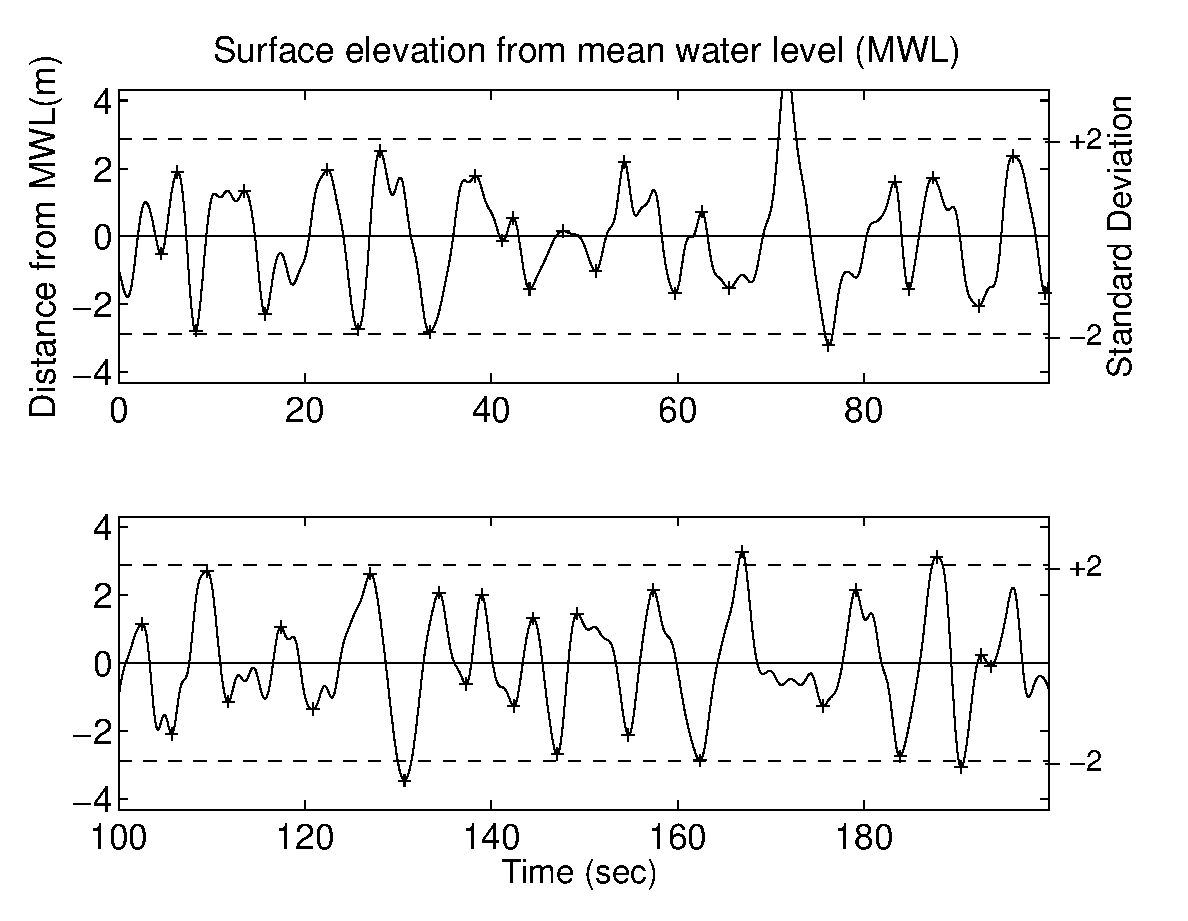
\includegraphics[width=\onefigwidth]{001f_sim}
%\psfig{figure=./Nyabilder/001f_sim.eps,width=\onefigwidth}
\vspace{-3mm}
\caption[Example of simulated wave profile]{A simulation
    from $S(\omega)$, a Torsethaugen spectrum with
    $H_{m_0}=6$~[m], $T_p=8$~[s].  Total number of points
    $=2000$, $\Delta t=0.1$~[s].}
\label{fig:simulation}
\end{figure}
  %-----

  We start by defining a frequency spectrum, $S(\omega)$, which will be
  used in many of the examples; we choose a Torsethaugen spectrum with
  the parameters $H_{m_0}=6$ [m], $T_p=8$ [s], describing significant wave
  height and primary peak period, respectively. The energy is divided
  between two peaks, corresponding to contributions from wind and swell;
  \cite{Torsethaugen1996Model}. % Torsethaugen 1996).
  \progname{} allows spectra to be defined simply by
  their parameters $H_{m_0}$ and $T_p$. The list in Section~\ref{s:ListOfSpectra} 
  helps to keep track of the different theoretical and empirical spectra we use in this tutorial. 
  \index[xentr]{spectrum!list of spectra used}

  %==============================================
  \subsection{Simulation from spectrum, estimation of spectrum}%---
  %==============================================
\index[xentr]{simulation!from spectrum}

  In Figure~\ref{fig:simulation}, plotted using {\tt waveplot},
  we have simulated a sample path from
  $S(\omega)$. \index[xcmds]{{\tt waveplot}}
 %The algorithm can equally well have the covariance function as input.
  The user specifies the number of wanted points in
  the simulation.  The following code in  \ML{}
  generates 200 seconds of data sampled with 10 Hz
  from the discussed spectrum. More on simulation can be found in
  Section~\ref{sec:simulationofGaussian}. \index[xcmds]{{\tt plotflag}}
{\small\begin{verbatim}
      Hm0 = 6; Tp = 8; plotflag = 1; clf
      ST = torsethaugen([],[Hm0 Tp],plotflag);
      dt = 0.1; N = 2000;
      xs = spec2sdat(ST,N,dt); clf
      waveplot(xs,'-')
\end{verbatim}}\index[xcmds]{{\tt spec2sdat}}

In a  common situation, data is given in form of a time
series, for which one wants to estimate the related spectrum.
We will now simulate 20 minutes of the signal sampled with 4~Hz,
find an estimate $S_{\mbox{\footnotesize est}}(\omega)$ and compare the
result to the original Torsethaugen spectrum $S(\omega)$.
The following code was used to generate Figure~\ref{fig:spectra},
where the original and estimated spectra are displayed. The maximum
lag size of the Parzen window function used (here 400) can be chosen
by the user or automatically by \progname{}. \index[xentr]{window!Parzen}
{\small\begin{verbatim}
      plotflag = 1; Fs = 4; clf
      dt = 1/Fs; N  = fix(20*60*Fs);
      xs = spec2sdat(ST,N,dt);
      STest = dat2spec(xs,400)
      plotspec(ST,plotflag), hold on
      plotspec(STest,plotflag,'--')
      axis([0 3 0 5]), hold off
\end{verbatim}}

    \index[xcmds]{{\tt plotspec}}

  %-----
  \begin{figure}[tbh]
    \centering
    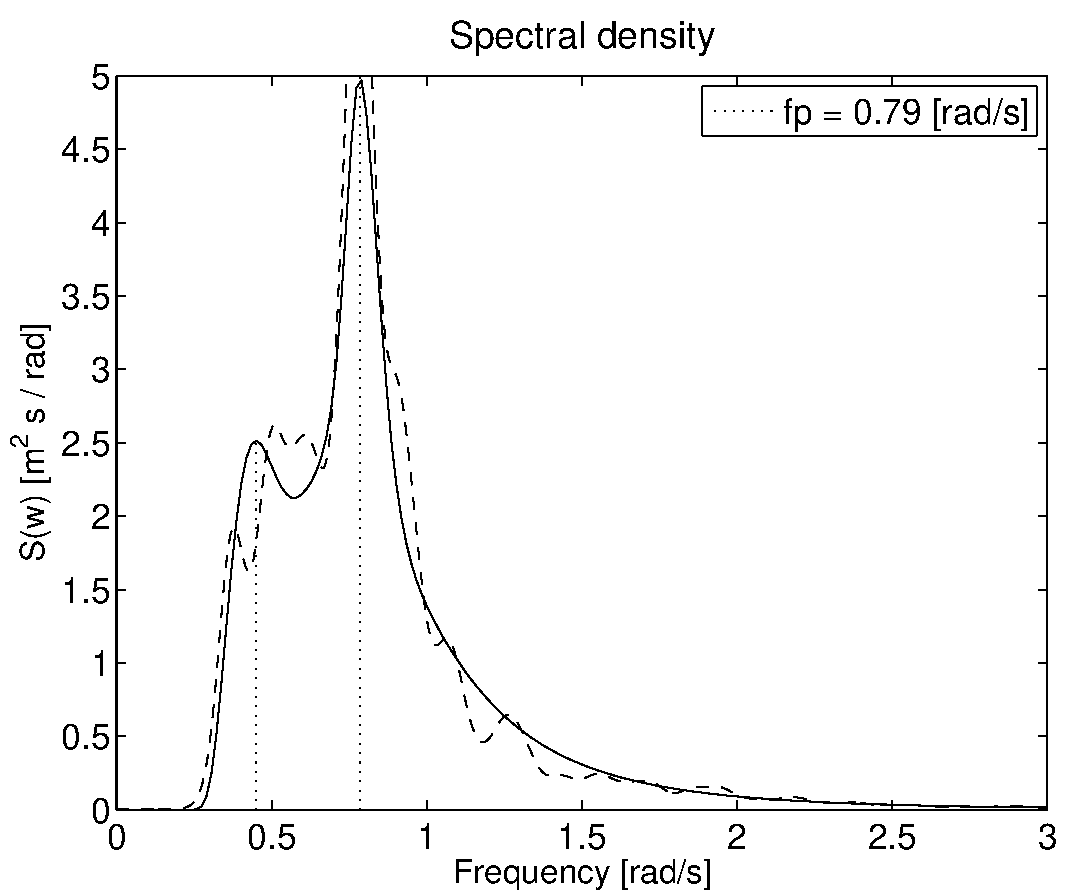
\includegraphics[width=\narrowfigwidth]{002f_spc}
\vspace{-3mm}
    \caption[Example of estimated spectrum]{Solid: 
      Thorsethaugen spectrum {\tt ST}.
  Dashed:  spectrum {\tt STest} estimated from
  data (20 minutes). % and 95\% confidence interval (dotted).
  Maximum lag size of Parzen window $=400$.}
  \label{fig:spectra}
  \end{figure}
  %-----
\label{page:torsethaugen}
  %-----
  %==============================================
  \subsection{Probability distributions of wave characteristics} %---
  %==============================================
  \progname{} gives the possibility to compute exact probability
  distributions for a number of wave characteristics, given a spectral
  density. A wave characteristic as, for example, wave period, can be
  defined in several ways, see Table~\ref{tab3_1}, page~\pageref{tab3_1}, in
  Chapter~\ref{cha:3}, and \progname{} allows the user to choose between
  a number of definitions: trough-to-crest, down-to-up crossing,
  up-to-up crossing, etc. In Chapter~\ref{cha:3} we analyse wave
  characteristics from observed data, and present some commonly used
  approximative distributions. Chapter~\ref{cha:4} describes how to use
  \progname{} to compute the exact theoretical distributions for
  all these wave characteristics in a
  Gaussian or transformed Gaussian model.

  In the numerical example, we consider the trough
  period, i.e.\ the down-to-up crossing definition. The wave periods
  can be extracted from the realization in Figure~\ref{fig:simulation}, and
  are shown as a histogram in Figure~\ref{fig:pdf}. This histogram may be
  compared to the theoretical density, calculated from the original
  spectrum $S(\omega)$, and from
  the estimated spectrum $S_{\mbox{\footnotesize est}}(\omega)$; see
  Figure~\ref{fig:pdf}. Recall that, for this spectrum,  $T_p=8$~[s].
  The figure shows the density for the half period; the
  results are in good agreement with that from the original spectrum. The
  following code lines are used to produced the presented figure. The
  different steps are: first extract half periods from the data by
  means of the routine \verb+dat2wa+ \index[xcmds]{{\tt dat2wa}}
  and store in the variable
  \verb+T+, then use \verb+spec2tpdf+ \index[xcmds]{{\tt spec2tpdf}}
  to calculate the theoretical
  distribution.
The parameter \verb+NIT+ determines the accuracy of the calculation.
  {\small\begin{verbatim}
        NIT = 3; paramt = [0 10 51]; clf
        dtyex = spec2tpdf(ST,[],'Tt',paramt,0,NIT);
        dtyest = spec2tpdf(STest,[],'Tt',paramt,0,NIT);
        [T, index] = dat2wa(xs,0,'d2u');
        histgrm(T,25,1,1), hold on
        pdfplot(dtyex), pdfplot(dtyest,'-.')
        axis([0 10 0 0.35]), hold off
\end{verbatim}}

%-----
\begin{figure}[tbh]
\centering
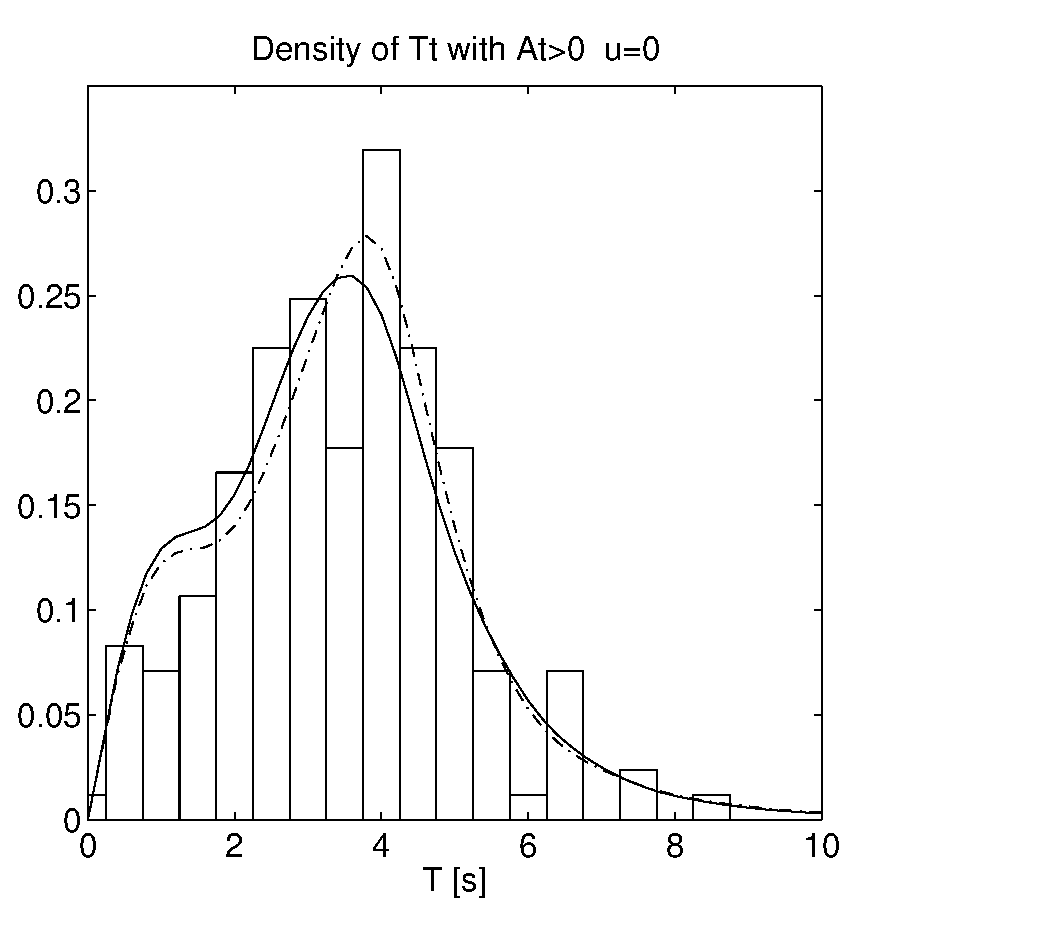
\includegraphics[width=\narrowfigwidth]{003f_pdf}
\vspace{-3mm}
\caption[Wave period, $T_{t}$, distribution]{
Pdf for wave  trough period for Torsethaugen spectrum {\tt ST} (solid line)
and estimated spectrum {\tt STest} (dash-dotted line).
The histogram shows the wave periods extracted from
the simulated data in Figure~\ref{fig:simulation}.}
\label{fig:pdf}
\end{figure}
%-----

%==============================================
\subsection{Directional spectra}\label{ss:dirspec}\index[xentr]{directional spectra}
\index[xentr]{spectrum!directional}
%==================
In \progname{} one finds means for evaluation and visualization of
directional spectra to model sea states with
waves coming from many different directions, that is
\[
   S(\omega,\theta)=S(\omega)\, D(\theta,\omega), \]
where $S(\omega)$ is a
frequency spectrum and $D(\theta,\omega)$ is a spreading function. A
number of common spreading functions can be chosen by the user.

One way of visualizing $S(\omega,\theta)$ is a polar plot. In
Figure~\ref{fig:directspect} we show the resulting directional spectrum
(solid line) for the Torsethaugen
spectrum  \index[xentr]{Torsethaugen!spectrum}
used above. The spreading \index[xentr]{spectrum!Torsethaugen}
function is of the \emph{cos-2s} type, that is (in the frequency
independent case),
\[
   D(\theta)=\frac{\Gamma(s+1)}{2\sqrt{\pi}\Gamma(s+1/2)}\cos^{2s}
    \left( \frac{\theta}{2} \right) \]
with $s\!\!=\!\!15$. Note that
the two peaks can be dis\-tinguished. The dash dotted line is the
corresponding result when the spreading function is frequency
dependent, cf.~\cite{KrogstadAndBarstow1999Directional}.
%Krogstad and Barstow (1999).

\begin{remark}``Wave direction''  is the direction from which waves are coming. 
\index[xentr]{wave!direction}
In \wf{} we adhere to the mathematical convention to count direction counter-clockwise 
from the positive $x$-axis. Thus, waves with direction 0$^o$ are coming from the East and 
waves with direction 90$^o$ are coming from the North, just the opposite to ocean standard. 
\end{remark}

Here are a few lines of code, which produce the graph of these
directional spectra with frequency independent and frequency dependent
spreading. The main directions are 90$^o$ and 0$^o$, respectively.
{\small\begin{verbatim}
    plotflag = 1; clf
    Nt = 101;   % number of angles
    th0 = pi/2; % primary direction of waves
    Sp = 15;    % spreading parameter
    D1 = spreading(Nt,'cos',th0,Sp,[],0); %frequency independent
    D12 = spreading(Nt,'cos',0,Sp,ST.w,1); %frequency dependent
    STD1 = mkdspec(ST,D1);  STD12 = mkdspec(ST,D12);
    plotspec(STD1,plotflag), hold on
    plotspec(STD12,plotflag,'-.'), hold off
\end{verbatim}}\index[xcmds]{{\tt mkdspec}}\index[xcmds]{{\tt plotspec}}

%-----
\begin{figure}[tbh]
  \centering
  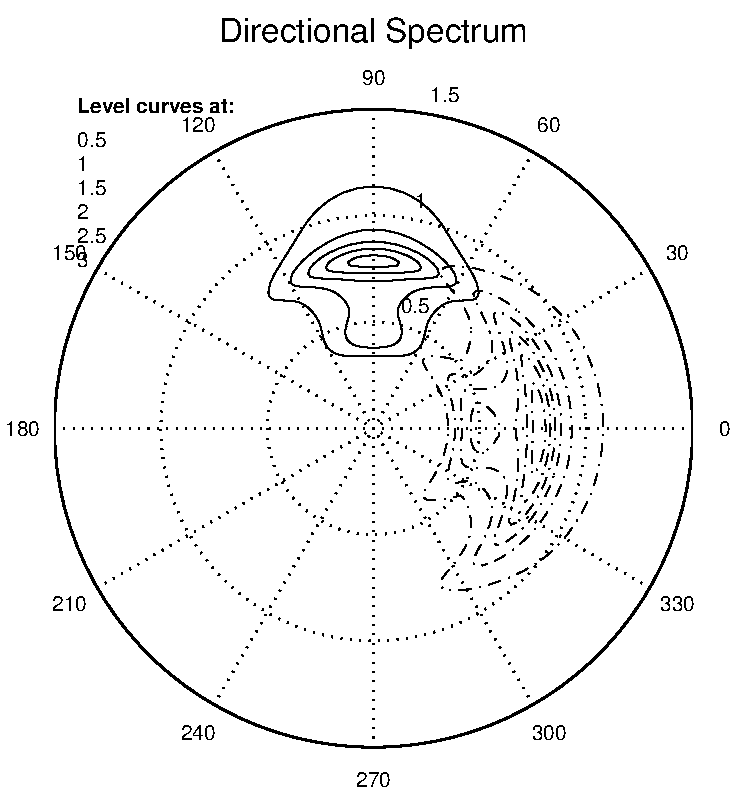
\includegraphics[width=\narrowfigwidth]{004f_drs}
\vspace{-3mm}
  \caption[Example of directional spectrum]{Directional spectrum.
  The frequency spectrum is a
  Torsethaugen spectrum and the spreading function is of \emph{cos-2s}
  type with $s = 15$. Solid line: directional spectrum with frequency
  independent spreading. Dash dotted line:
  directional spectrum, using frequency dependent spreading function.}
  \label{fig:directspect}
  \end{figure}
 %------

We finish the section with 20 seconds of simulated sea surfaces on 512[m] by 1024[m]
for a sea with directional spectra {\tt STD1} and {\tt STD12}. The
routine \verb+spec2field+ is used for simulation and the parameters 
for the simulation in space and time \index[xcmds]{{\tt simoptset}} 
are defined by the options function \verb+simoptset+. 
{\small\begin{verbatim}
    rng('default'); clf
    opt = simoptset('Nt',20,'dt',1,'Nu',1024','du',1,'Nv',512,'dv',1)
    W1 = spec2field(STD1,opt);
    W12 = spec2field(STD12,opt)
    
    W12 = struct with fields:
    Z: [512 x 1024 x 20 double]
    y: [1024 x 1 double]
    x: [512 x 1 double]
    t: [20 x 1 double]
\end{verbatim}}
\noindent
\index[xentr]{simulation!of sea surface}
\index[xcmds]{{\tt spec2field}}\index[xcmds]{{\tt simoptset}}
\index[xcmds]{{\tt seamovie}}

The generated space-time fields can be presented and optionally 
saved as a movie by the routine \verb+seamovie+. 
Specifying a file name saves the movie in avi-format, as for {\tt Movie12}.  
{\small\begin{verbatim}
    figure(1); clf
    Movie1 = seamovie(W1,1);
    figure(2); clf
    Movie12 = seamovie(W12,1,'GaussianSea12.avi')
\end{verbatim}

The last frame of the movies are shown in 
Figures~\ref{fig:00sima}-\ref{fig:00simb} and one can see that
waves are coming from different directions. However,
frequency dependent spreading leads to a more irregular
surface, so the orientation of waves is less transparent.
From the figures it is not easy to deduce that
both sea surfaces have the same period distribution, but
it is more obvious that the wavelength distributions are different.

\begin{figure}
  \centerline{
%\resizebox{\defwidth}{!}{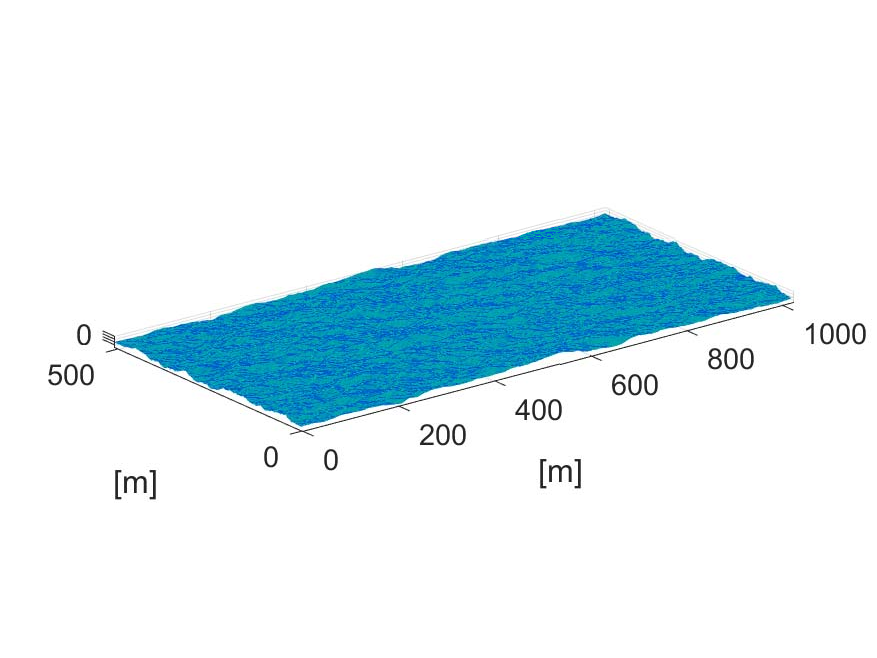
\includegraphics{fig_hav1aaa}}
\resizebox{0.95\textwidth}{!}{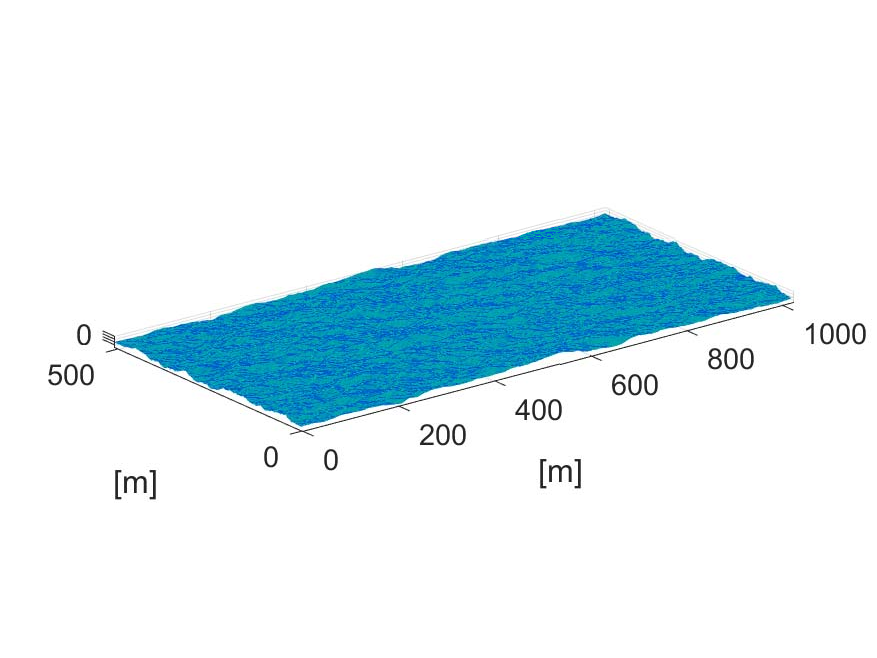
\includegraphics{fig_hav1aaa}}}
\vspace{-3mm}
\caption[Gaussian sea surface, frequency independent spreading]{Gaussian 
sea surface, 512 [m] by 1024 [m], with 
directional spectrum {\tt SD1}, spreading independent of frequency, waves from North.}
\label{fig:00sima}
\end{figure}
\begin{figure}
\centerline{
\resizebox{0.95\textwidth}{!}{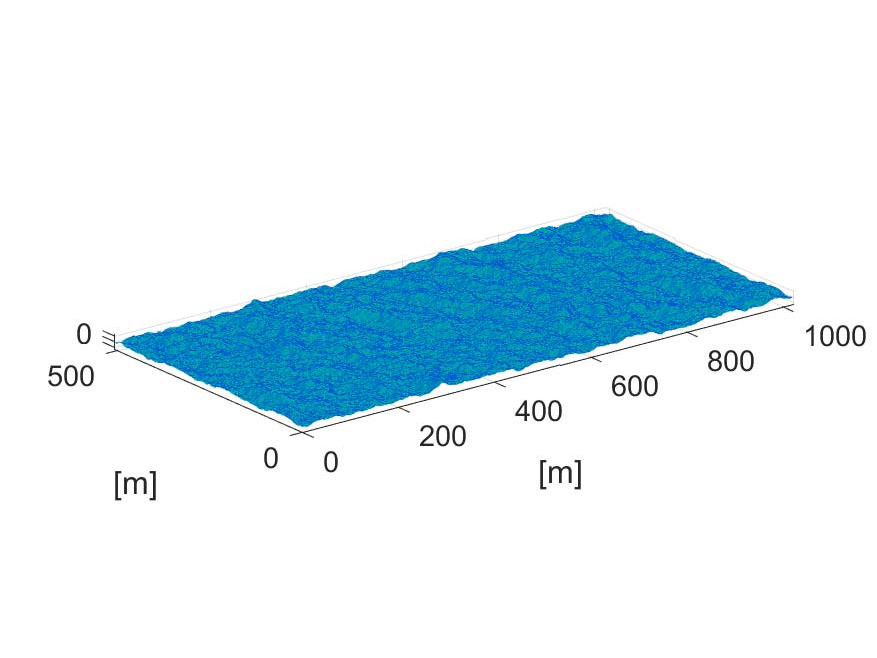
\includegraphics{fig_hav2aaa}}
}
\vspace{-3mm}
\caption[Gaussian sea surface, frequency dependent spreading]{Gaussian 
sea surface, 512 [m] by 1024 [m], with 
directional spectrum {\tt SD12}, frequency dependent spreading, waves from East.}
\label{fig:00simb}
\end{figure}

%==============================================
\subsection{Fatigue, load cycles, and Markov models}%---
%==============================================
In fatigue applications the exact sample path is not important, but
only the peaks and troughs of the load, called the  turning
points (TP). From these one can extract load cycles, from
which damage calculations and fatigue life predictions can be
performed. In \progname{}
there are numerous routines for evaluating fatigue measured loads, as
well as making theoretical calculations of distributions that are
important for fatigue evaluation.  A powerful technique when
analysing loads is to use Markov models as approximations, especially
to model the sequence of turning points by a Markov chain. For such
models there
exist many explicit results. Here, we will use this Markov
approximation for computing the intensity of rainflow cycles and
trough-to-crest cycles for the Gaussian model with spectrum from
Figure~\ref{fig:spectra}.

For fatigue analysis the rainflow cycle, defined in
Figure~\ref{FigRFCdef} in Chapter~\ref{cha:5}, is often used.
The Markov model is defined by the min-to-max pdf, which is obtained
from the power spectral density by using approximations in Slepian
model processes, see e.g.\
\cite{LindgrenAndRychlik1991Slepian} %LiRy91} %Lindgren and Rychlik~(1991)
and references therein. Chapter~\ref{cha:4} describes how \progname{}
routines can be used to find the min-to-max distribution for Gaussian loads.
For the Markov model, there is an explicit
solution for the intensity of rainflow cycles, see
\cite{FrendahlAndRychlik1993Rainflow}. \index[xentr]{min-to-max!pdf}
%,FrRy93}. %Frendahl and Rychlik~(1993).
By using the routines in \progname{} the intensity of rainflow cycles can be
found using Markov approximation; see Figure~\ref{fig:rainflow2}, where
also the rainflow cycles found in the simulated load signal are
shown. The figure has been plotted using the following commands:
{\small\begin{verbatim}
    paramu = [-6 6 61];
    frfc = spec2cmat(ST,[],'rfc',[],paramu);
    pdfplot(frfc); hold on
    tp = dat2tp(xs);      rfc = tp2rfc(tp);
    plot(rfc(:,2),rfc(:,1),'.'); hold off
\end{verbatim}}\index[xcmds]{{\tt spec2cmat}}
    \index[xcmds]{{\tt dat2tp}}\index[xcmds]{{\tt tp2rfc}}

%----- Figure
%-----
  \begin{figure}[tbh]
\centering
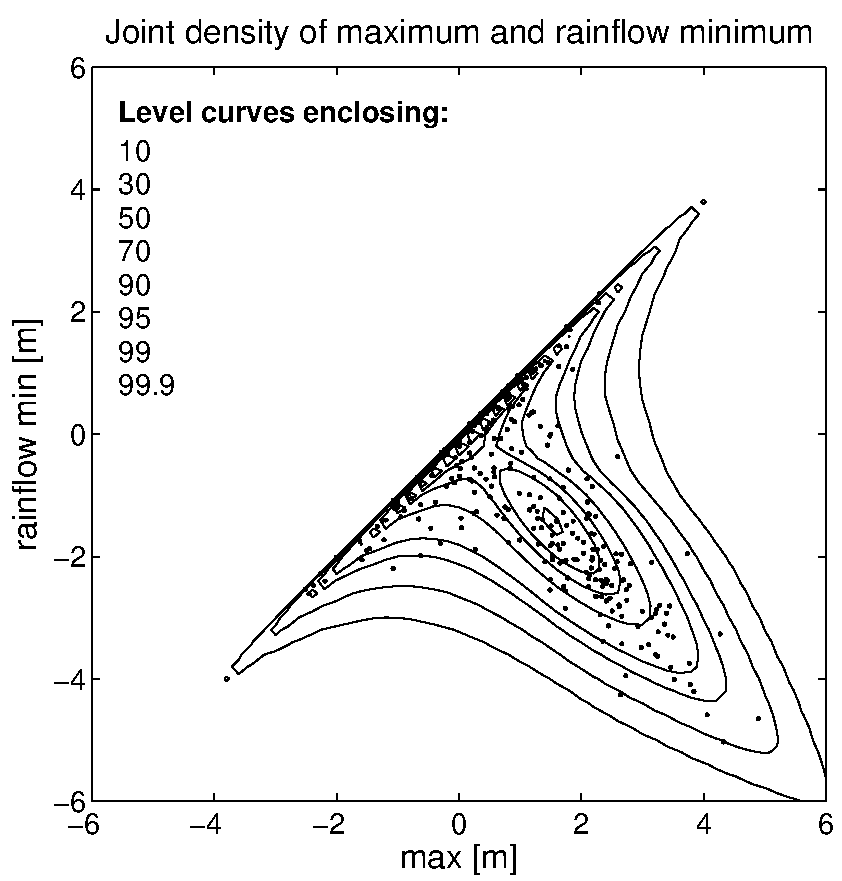
\includegraphics[width=\narrowfigwidth]{006f_rfc}
\vspace{-3mm}
\caption[Intensity of rainflow cycles]{Intensity of rainflow cycles
computed from the power spectrum through
  Markov approximation, compared with cycles found in the
  simulation. }
\label{fig:rainflow2}
\end{figure}
  %-----
  %----- End Figure

  \noindent
  The \progname{} toolbox also contains routines for computing the intensity
  of rainflow cycles in more complex load processes, for example
  for a switching Markov chain of turning points, {\tt TP}. Details on fatigue load analysis
are given in Chapter~\ref{cha:5}.

%==============================================
\subsection{Statistical extreme value analysis}\label{sec:extreme_example} %---
%==============================================
The {\sc Wafo}-toolbox contains almost 600 routines for general
statistical analysis, description, plotting, and simulation.
In Chapter~\ref{cha:6} we describe some routines which are particularly
important for wave and fatigue analysis, related to statistics of extremes.
These are based on the generalized extreme value (GEV) and generalized Pareto
distribution (GPD), combined with the peaks over threshold (POT) method.
\index[xentr]{Generalized Extreme Value!distribution, GEV}
\index[xentr]{Generalized Pareto!distribution, GPD}
As an example we show an analysis of wave elevation data from the
Poseidon platform in the Japan Sea. Data from about 23 hours of registration
are stored in the data set {\tt yura87}, taken with a 1~Hz sampling rate.
We first load and plot, in Figure~\ref{fig:yura87},
part of the data and calculate the maximum over 5 minute periods.
{\small\begin{verbatim}
      xn = load('yura87.dat'); subplot(211);
      plot(xn(1:30:end,1)/3600,xn(1:30:end,2),'.')
      title('Water level'), ylabel('m')
      yura = xn(1:85500,2);
      yura = reshape(yura,300,285);
      maxyura = max(yura); subplot(212)
      plot(xn(300:300:85500,1)/3600,maxyura,'.')
      xlabel('Time (h)'), ylabel('m')
      title('Maximum 5 min water level')
\end{verbatim}}

%----- Figure
%-----
  \begin{figure}[tbh]
\centering
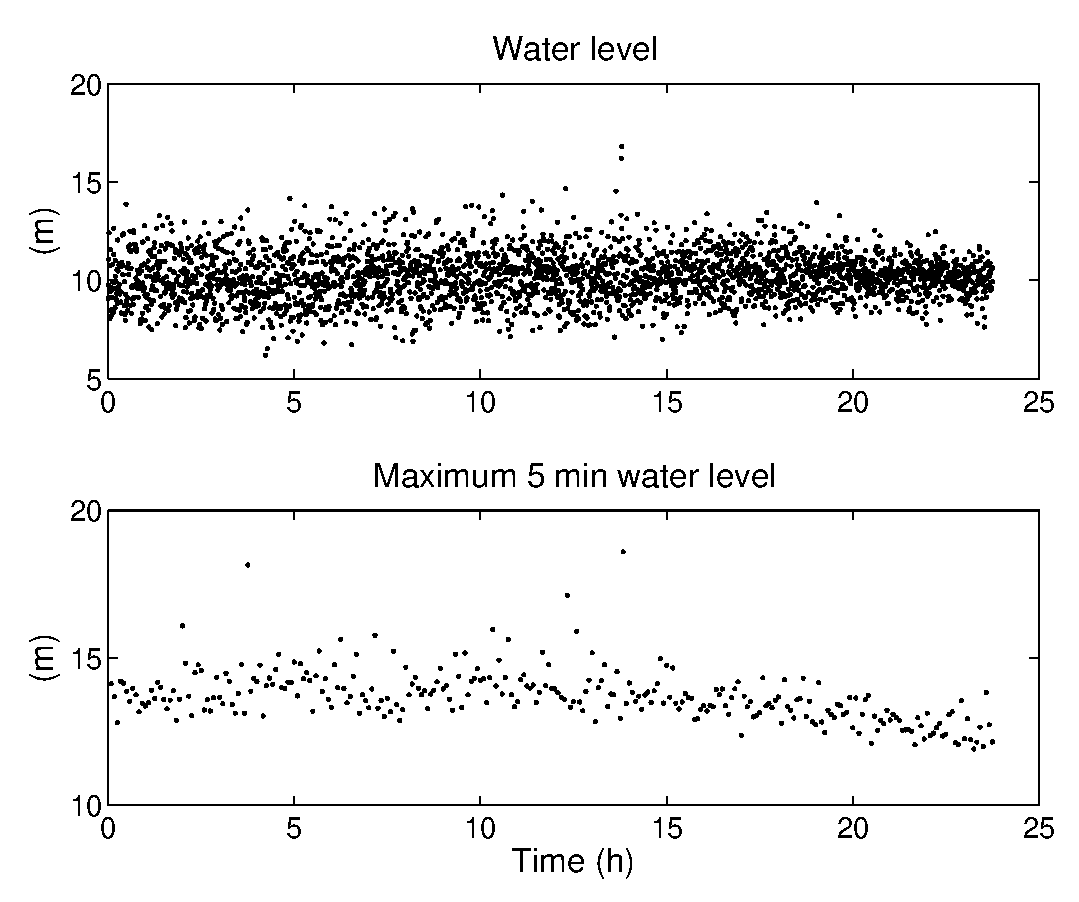
\includegraphics[width=0.85\textwidth]{007f_yura}
\vspace{-3mm}
\caption[Water level in the Japan Sea]{Water level variation in the Japan Sea
from the data set {\tt yura87} and maxima over 5~minute periods.}
\label{fig:yura87}
\end{figure}
  %-----
  %----- End Figure

\begin{figure}[tbh]
\centering
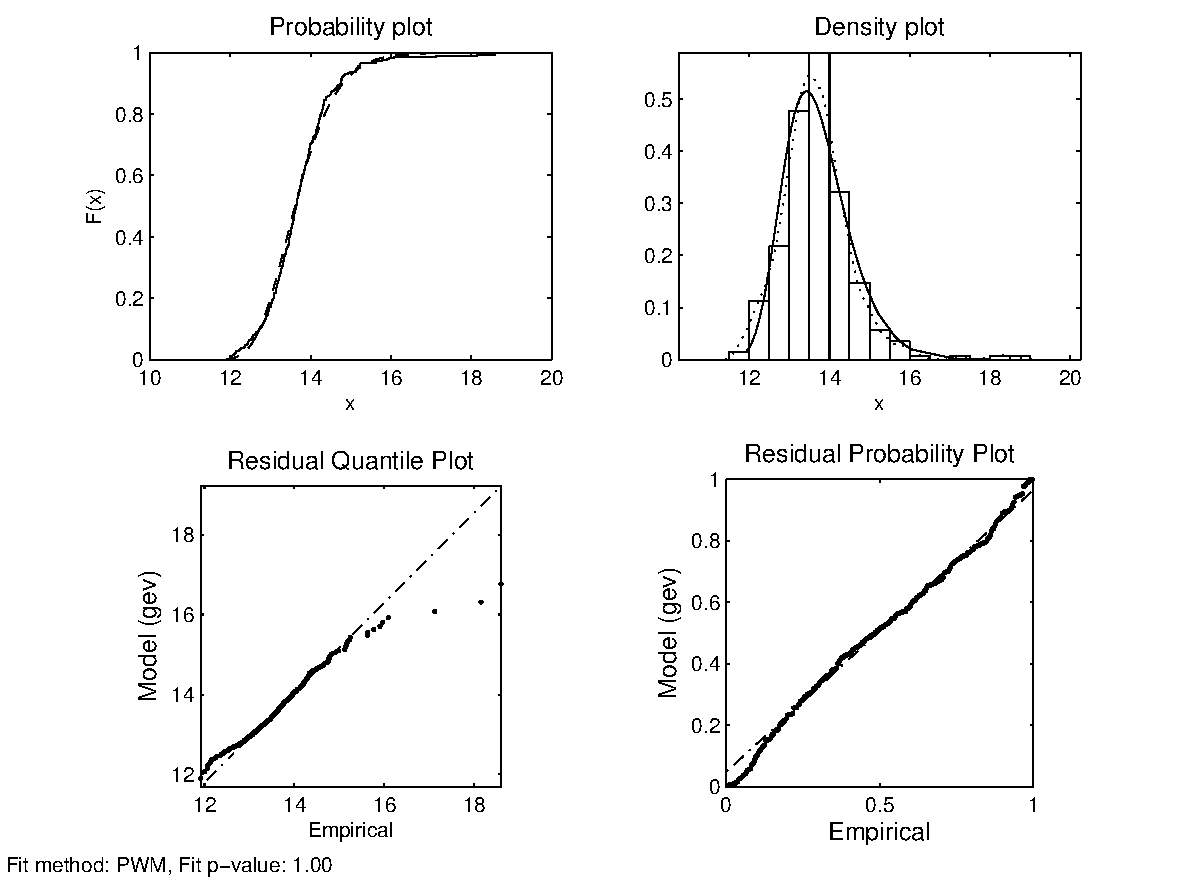
\includegraphics[width=0.85\textwidth]{008f_yuragev}
%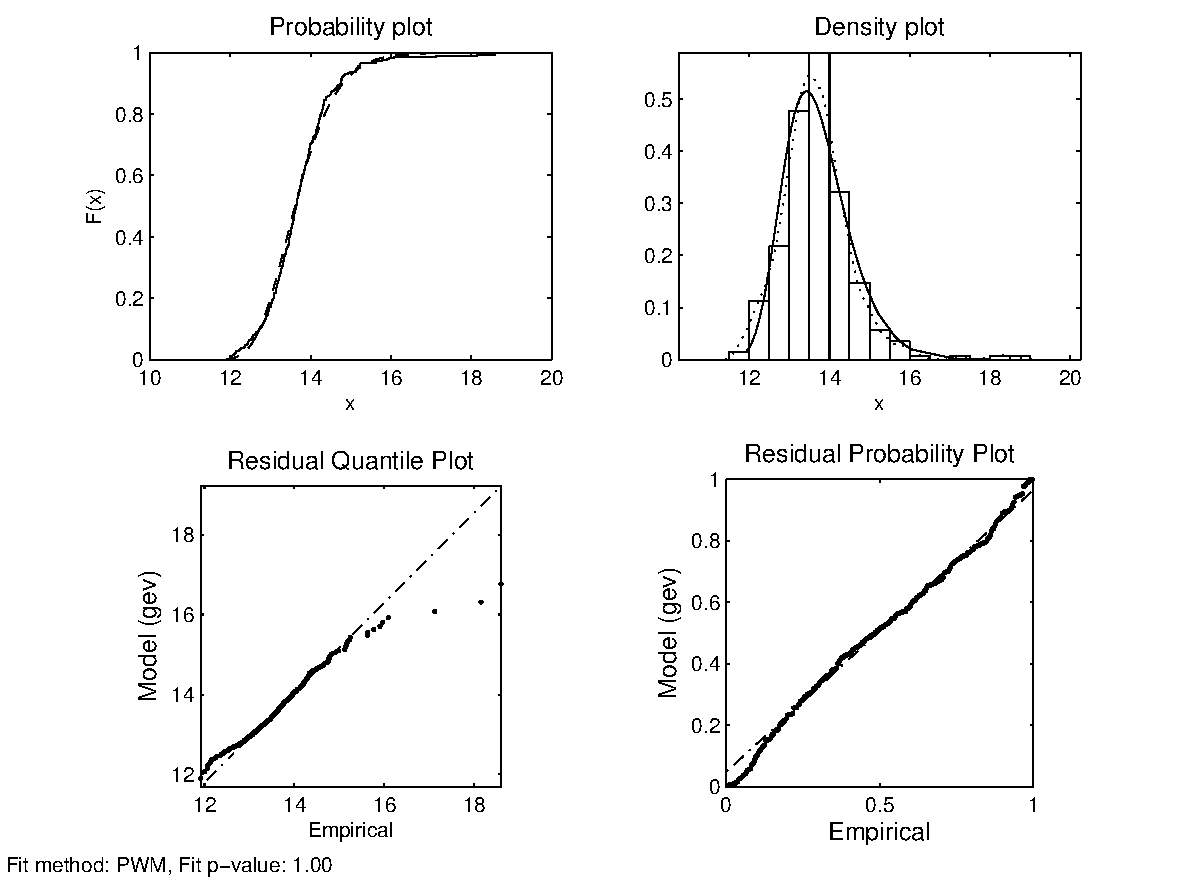
\includegraphics[width=100mm]{008f_yuragev}
\vspace{-3mm}
\caption[Extreme value analysis of {\tt yura87}]
{Diagnostic plots of GEV extreme value analysis of {\tt yura87}.}
\label{fig:yuragev}
\end{figure}

It is clear from the figures that there is a trend in the data, with
decreasing spreading with time. In Chapter~\ref{cha:5} we will deal with
that problem; here we make a crude extreme value analysis, by fitting a
GEV distribution to the sequence of 5 minute maxima,
simply by issuing the commands
{\small \begin{verbatim}
      phat = fitgev(maxyura,'plotflag',1);
\end{verbatim}}\index[xcmds]{{\tt fitgev}}
%This results in 

Figure~\ref{fig:yuragev}  shows cumulative distribution
and density of the fitted GEV distribution together with diagnostic
plots of empirical and model quantiles. The non-stationarity
gives a very bad fit in the upper tail of the distribution. The fitted GEV
has shape parameter $0.1$, with a 95\% confidence interval $(0.01, 0.18)$.
%\vspace{10mm}
%\newpage

%\clearpage
%\vspace{15cm}
%~

\section{Spectra used in the tutorial}\label{s:ListOfSpectra}
In this tutorial we illustrate the routines on many different wave and load spectra. 
Some are empirical, estimated from wave data, others are theoretical spectra 
suggested in the literature as suitable for special wave conditions. The following 
list and name convention 
should help the reader to keep track of the different types through the 
many examples in the next chapters.   The notation {\tt SXest} will occasionally be used 
for estimated spectra. 

\subsection{SG, Empirical spectrum from waves in {\tt gfaksr89.dat}}
Bi-modall spectrum {\tt SG} estimated at the Gullfaks~C platform at 2.5\:[Hz], 39\,000 data poins. 
This spectrum is used in Examples~\ref{Ex_preliminary_analysis}--\ref{Crest-trough-from-min-max}. 

\subsection{SJ, Theoretical {\sc Jonswap} spectrum}
Theoretical uni-modal {\sc Jonswap} spectrum {\tt SJ} designed for North Sea waves. 
This spectrum is used in Examples~\ref{Ex_sea_spectra}, \ref{Seamovieforexport}, and \ref{Ex_wave_parameters}.

\subsection{SS, Empirical spectrum from waves in {\tt sea.dat}}
Bi-modal spectrum {\tt SS}, estimated from shallow water wave data, 
sample rate 4\:[Hz], 9\,524 data points. This spectrum is used in Examples~\ref{Ex_sea_statistics}, 
\ref{Ex_sea_simulation}, \ref{rayleighapproximation}, \ref{Ex_Seadatawavedistributions}.

\subsection{ST, Theoretical {\sc Torsethaugen} spectrum}
Theoretical bi-modal {\sc Torsethaugen} spectrum {\tt ST} designed for mixed sea 
with wind waves and swell. This spectrum is used in Example~\ref{Ex_Torseth}.

% \subsection{SY, Empirical spectrum from waves in {\tt yura87.dat}}
%Uni-modal spectrum {\tt SY}, estimated from wave data, sample rate 1\:[Hz], 85\,547 data points.

\clearpage
%\newpage
\section{Datastructures}\label{sec:datastructures}
\index[xentr]{datastructures}\index[xentr]{structured array}
\vspace{-3mm}
{\small\begin{verbatim}
help datastructures

 DATASTRUCTURES of spectrum (S), covariance function (cvf)
 and probability density (pdf) in WAFO

  To represent spectra, covariance functions and probability
  density functions in WAFO, the MATLAB datatype 'structured
  array' is used. Here follows a list of the fields in
  the struct representing S, cvf and pdf, respectively.

  Spectrum structure
  ~~~~~~~~~~~~~~~~~~
   Requisite fields:
    .type  String: 'freq', 'dir', 'k2d', k1d', 'encdir', 'enc'.
    .S     Spectrum values (size=[nf 1] or [np nf]).
    .w OR .f OR .k Frequency/wave number lag, length nf.
    .tr    Transformation function (default [] (none)).
    .h     Water depth (default inf).
    .norm  Normalization flag, Logical 1 if S is normalized,
           0 if not.
    .note  Memorandum string.
    .date  Date and time of creation or change.
   Type-specific fields:
    .k2    Second dim. wave number lag,
           if .type='k2d', 'rotk2d', length np.
    .theta Angular lags, if .type='dir', 'rotdir' or 'encdir',
           length np.
    .v     Ship speed, if .type = 'enc' or 'encdir'.
    .phi   angle of rotation of the coordinate system
           (counter-clockwise) e.g. azimuth of a ship.

  See also  createspec, plotspec

  Covariance function (cvf) structure
  ~~~~~~~~~~~~~~~~~~~~~~~~~~~~~~~~~~~
    .R     Covariance function values, size [ny nx nt],
           all singleton dim. removed.
    .x     Lag of first space dimension, length nx.
    .y     Lag of second space dimension, length ny.
    .t     Time lag, length nt.
    .h     Water depth.
    .tr    Transformation function.
    .type  'enc', 'rot' or 'none'.
    .v     Ship speed, if .type='enc' .
    .phi   Rotation of coordinate system, e.g. direction of ship.
    .norm  Normalization flag, Logical 1 if autocorrelation,
           0 if covariance.
    .Rx ... .Rtttt   Obvious derivatives of .R.
    .note  Memorandum string.
    .date  Date and time of creation or change.

  See also  createcov, spec2cov, cov2spec, covplot

  Probability density function (pdf) structure
  ~~~~~~~~~~~~~~~~~~~~~~~~~~~~~~~~~~~~~~~~~~~~
  Describing a density of n variables:
    .f     Probability density function values,
           (n-dimensional matrix).
    .x     Cell array of vectors defining grid for variables,
           (n cells).
    .labx  Cell array of label strings for the variables,
           (n cells).
    .title Title string.
    .note  Memorandum string.

  See also  createpdf, pdfplot
\end{verbatim}
}

%\bibliography{wafoBibliography}

%%% Local Variables:
%%% mode: latex
%%% TeX-master: "wafomanual"
%%% End:

%\svnInfo $Id: Ch2_2017.tex 67 2017-09-12 08:21:29Z Georg Lindgren $  
%$
%
\chapter{Random waves and loads}
\label{cha:rand-loads-stoch}\label{cha:2}

In this chapter we present some tools for analysis of random functions
with respect to their correlation, spectral, and distributional
properties. We first give a brief introduction to the theory of Gaussian
processes and then we present programs in \progname{},
which can be used to analyse random functions. For deeper insight in the theory 
we refer to \cite{Lindgren2013,LindgrenRootzenSandsten2014}.

The presentation will be organized in three examples:
Example~\ref{Ex_sea_statistics}
is devoted to estimation of different parameters in the model,
Example~\ref{Ex_sea_spectra}
deals with spectral densities and
Example~\ref{Ex_sea_simulation}
presents the use of \progname{} to simulate samples of a Gaussian process.
The commands, collected in \verb+Chapter2.m+, run in less than
5~seconds on a 3.60~GHz 64 bit PC with Windows 10; add another two minutes 
for the display of simulated wave fields.

\section{Introduction and preliminary analysis}
\label{sec:intr-prel-analys}\label{sect2.1}
The functions we shall analyse can be measured stresses or strains,
which we call loads, or other measurements, where waves on the sea
surface is one of the most important examples.
We assume that the measured data are given in one of the following  forms:

\begin{enumerate}
\item In the time domain, as measurements of a response function
denoted by $x(t)$, $0\le t\le T$, where $t$ is time and $T$ is the
duration of the measurements. The  $x(t)$-function is usually
sampled with a fixed sampling frequency and a given resolution,
i.e.\ the values of $x(t)$ are also discretised. The effects of
sampling can not always be neglected in estimation of parameters
or distributions. We assume that measured functions are saved as a
two column ASCII or {\tt mat} file.

Some general properties of measured functions can be
summarized by using a few simple characteristics. Those are the
\emph{mean} $m$, defined as the average of all values, the
\emph{standard deviation} $\sigma$, and the \emph{variance}
$\sigma^2$, which measure the variability around the mean in linear
and quadratic scale. These quantities are estimated by
\begin{eqnarray}
m &=&1/T\,\int_0^T x(t)\, \rd t, \\
\sigma^2 &=& 1/T\,\int_0^T (x(t)-m)^2\, \rd t,
\end{eqnarray}
for a continuous recording or by corresponding sums for a sampled series.

\item In the frequency domain, as a power spectrum, which is an
important mode in systems analysis. This means that the signal
is represented by a Fourier series,
\begin{equation}
x(t)\approx
m + \sum_{i=1}^N a_i\cos(\omega_i\,t)+b_i
\sin(\omega_i\,t),
\label{eqn:fourier_series}
\end{equation}
where $\omega_i=i\cdot 2\pi/T$ are angular
frequencies,
$m$ is the mean of the signal and $a_i,b_i$ are Fourier coefficients.

\item Another important way to represent a load sequence is by means of
the \emph{crossing spectrum}\index[xentr]{crossing spectrum}
\index[xentr]{spectrum!crossing} or
\emph{ crossing intensity},
\index[xentr]{crossing intensity}
$\mu(u)$ = the intensity of
upcrossings = average number of upcrossings per time unit, of a
level $u$ by $x(t)$ as a function of $u$,
see further in Section~\ref{subsec:crossing_intensity}.
The \emph{mean frequency}\index[xentr]{mean frequency}
$f_0$ is usually defined as the number of
times $x(t)$ crosses upwards (upcrosses) the mean level  $m$
normalized by the length of the observation interval $T$, i.e.\
$f_0=\mu(m)$. An alternative definition,\footnote{Still another
  definition, to be used in Chapter~\ref{cha:5},
is that $f_0$ is the average number of completed load cycles per time
unit.} which we prefer to use is that $f_0=\max \mu(u))$, i.e.
it is equal to the maximum of $\mu(u)$.
The \emph{irregularity factor}\index[xentr]{irregularity factor}
$\alpha$ is defined as the mean frequency $f_0$
divided by the intensity of local maxima (``intensity of cycles'', i.e.\
the average number of local maxima per time unit)
in $x(t)$. Note, a small $\alpha$ means an irregular process,
$0 < \alpha \leq 1$.
\end{enumerate}

\begin{rtex}{Ex_sea_statistics}{Sea data}\label{pageseadat}
In this example we use a series with wave data {\tt sea.dat}
with time argument in the first column and function values in
the second column. The data used in the examples are wave measurements
at shallow water location, sampled with a sampling frequency
of~4~Hz, and the units of measurement are seconds and meters, respectively.
The file {\tt sea.dat} is loaded into \ML{} and after the mean
value has been subtracted the data are saved in the two column matrix
{\tt xx}.
{\small\begin{verbatim}
      xx = load('sea.dat');
      me = mean(xx(:,2))
      sa = std(xx(:,2))
      xx(:,2) = xx(:,2) - me;
      lc = dat2lc(xx);
      plotflag = 2;
      lcplot(lc,plotflag,0,sa)
\end{verbatim}}\index[xcmds]{{\tt dat2lc}}\index[xcmds]{{\tt lcplot}}
Here {\tt me} and {\tt sa} are the mean and standard deviation of the signal,
respectively. The variable {\tt lc} is a two column matrix with
levels in the first column and the number of upcrossing of the level in
the second. In Figure~\ref{fig1_cr} the number of upcrossings of
{\tt xx} is plotted and compared with an estimation based on the
assumption that {\tt xx} is a realization of a Gaussian sea.

Next, we compute the mean frequency as the average number of upcrossings
per time unit of the mean level (= 0); this may require interpolation in the
crossing intensity curve, as follows.
{\small\begin{verbatim}
      T = max(xx(:,1))-min(xx(:,1))
      f0 = interp1(lc(:,1),lc(:,2),0)/T
         % zero up-crossing frequency
\end{verbatim}}

\begin{figure}[tbh]
\centering
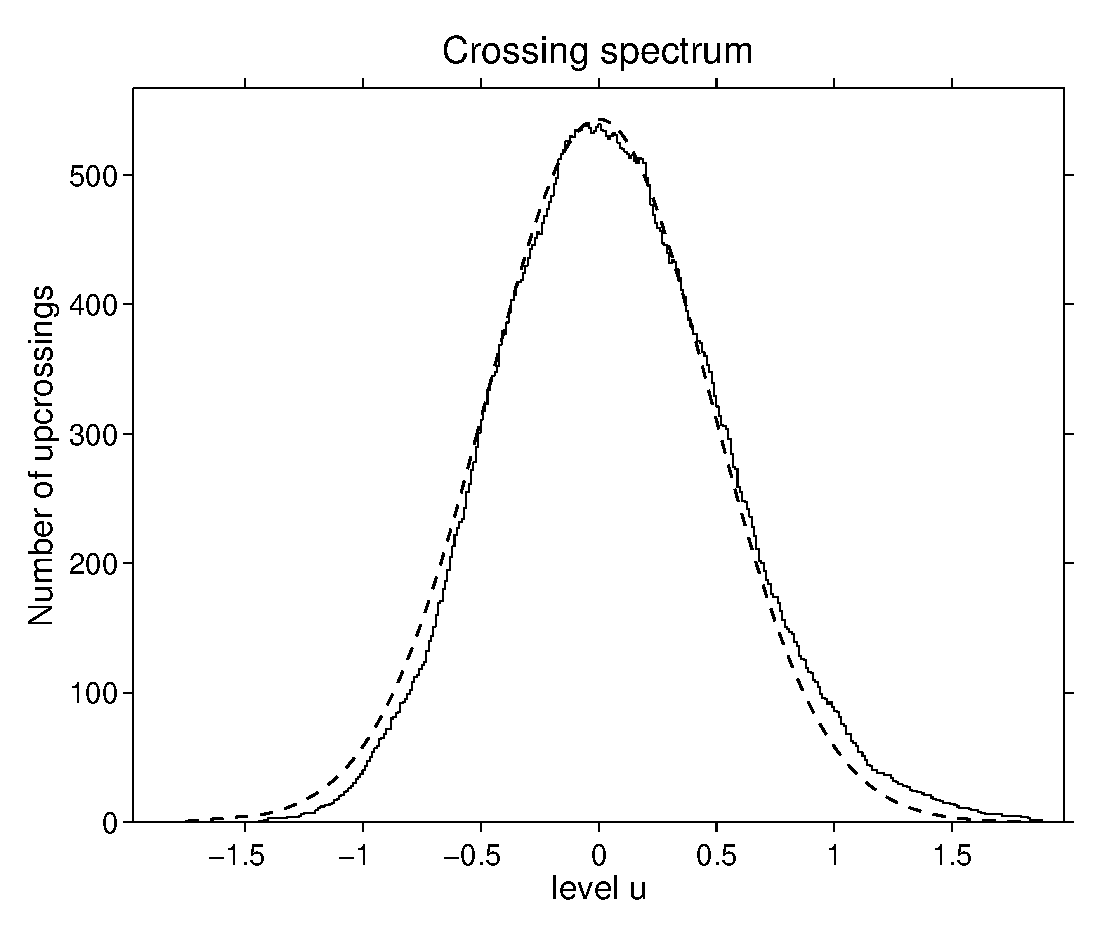
\includegraphics[width=\narrowfigwidth]{fig1_cr}
\vspace{-3mm}
\caption[Example of crossing spectrum]{
The observed crossings intensity compared with the theoretically expected for
Gaussian signals, see (\ref{eq:rice}).}
\label{fig1_cr}
\end{figure}
The process of fatigue damage accumulation depends only on the values
and the order of the local extremes in the load. The sequence of local
extremes is called the \emph{sequence of turning points}.
\index[xentr]{turning points}
\index[xentr]{sequence of turning points} It is a two
column matrix with time for the extremes in the first column and the
values of the extremes in the second.
{\small\begin{verbatim}
      tp = dat2tp(xx);
      fm = length(tp)/(2*T)            % frequency of maxima
      alfa = f0/fm
\end{verbatim}}\index[xcmds]{{\tt dat2tp}}

Here {\tt alfa} is the irregularity factor. Note that {\tt length(tp)} is
equal to the number of local maxima and minima and hence we have a
factor~2 in the expression for {\tt fm}.
\end{rtex}

We finish this section with some remarks about the quality
of the measured data. Especially sea surface measurements can be
of poor quality.
It is always good practice to visually examine the data
before the analysis to get an impression of the quality,
non-linearities and narrow-bandedness of the data.

\begin{cex}{Ex_sea_statistics}\label{page:spurious}
First we shall plot the data {\tt xx} and zoom in on a specific region.
A part of the sea data is presented in Figure~\ref{fig2-1}
obtained by the following commands.
 {\small\begin{verbatim}
      waveplot(xx,tp,'k-','*',1,1)
      axis([0 2 -inf inf])
\end{verbatim}}\index[xcmds]{{\tt waveplot}}

\begin{figure}
\centering
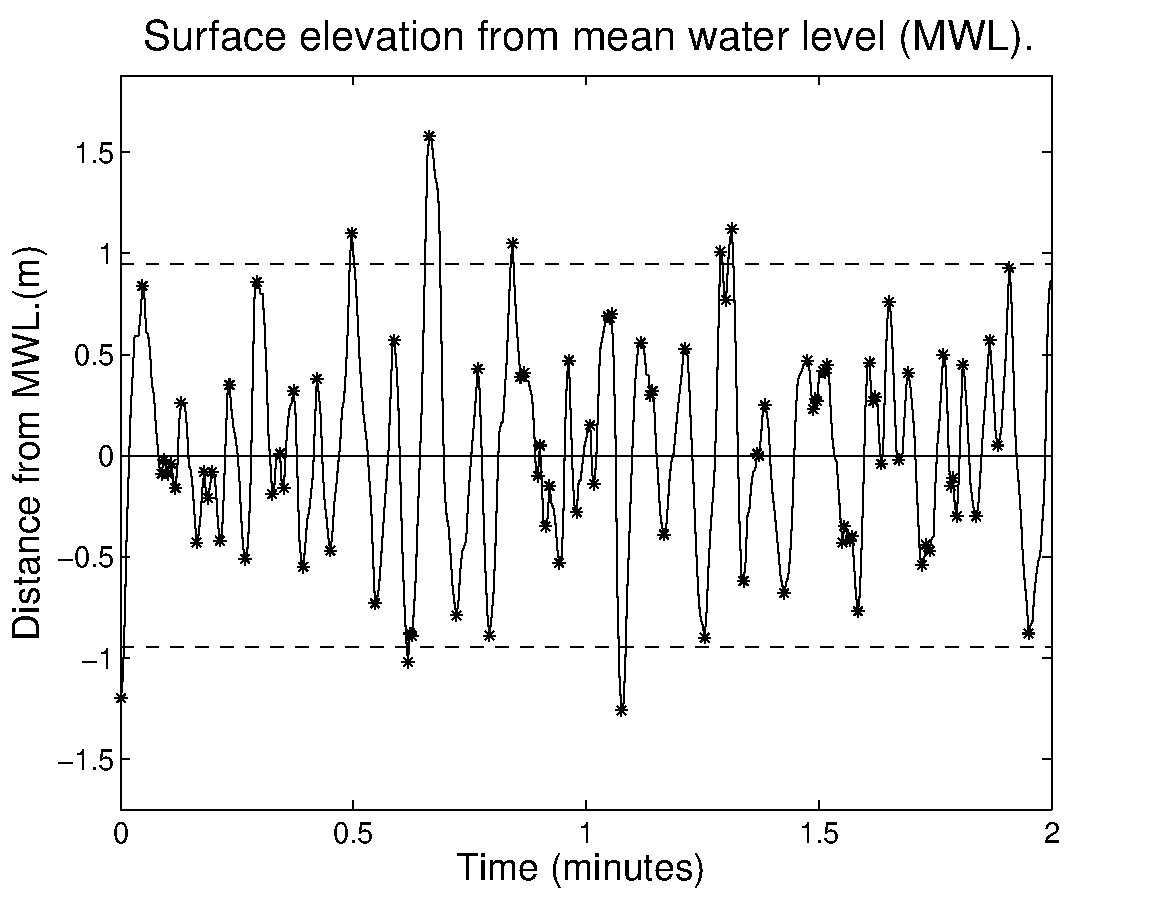
\includegraphics[width=\narrowfigwidth]{figure_Ch2_1}
\vspace{-3mm}
\caption[Plotting sea data and local turning points]{A part of
the sea data with turning points marked as stars.}
\label{fig2-1}
\end{figure}

However, if the amount of data is too large for visual examination, or
if one wants a more objective measure of the quality of
the data, one could use the following empirical criteria:
\begin{itemize}\setlength\itemsep{-1mm}
\item $x'(t) < 5$ [m/s], since the raising speed of
Gaussian waves rarely exceeds 5 [m/s],
\item $x''(t) < 9.81/2$, $[m/s^2]$ which is the limiting maximum
acceleration of Stokes waves,
\item if the signal is constant in some intervals, then this will add high
frequencies to the estimated spectral density; constant data may occur if
the measuring device is blocked during some period of time.
\end{itemize}

\noindent
To find possible spurious points of the dataset use the following commands.
{\small\begin{verbatim}
      dt = diff(xx(1:2,1));
      dcrit = 5*dt;
      ddcrit = 9.81/2*dt*dt;
      zcrit = 0;
      [inds indg] = findoutliers(xx,zcrit,dcrit,ddcrit);
\end{verbatim}}\index[xcmds]{{\tt findoutliers}}

\noindent
The program will give the following list when used on the sea data.
{\small\begin{verbatim}
Found 0 missing points
Found 0 spurious positive jumps of Dx
Found 0 spurious negative jumps of Dx
Found 37 spurious positive jumps of D^2x
Found 200 spurious negative jumps of D^2x
Found 244 consecutive equal values
Found the total of 1152 spurious points
\end{verbatim}}

The values for {\tt zcrit}, {\tt dcrit} and  {\tt ddcrit}
can be chosen more carefully. One must be careful using the
criteria for extreme value analysis, because
it might remove extreme waves that belong to the data and
are not spurious. However, small changes of the
constants are usually not so crucial. As seen from the
transcripts from the program a total of 1152 points are
found to be spurious which is approximately 12~\% of the data.
Based on this one may classify the datasets into good,
reasonable, poor, and useless. Obviously, uncritical use of
data may lead to unsatisfactory results. We return to this
problem when discussing methods to reconstruct the data.
\end{cex}

\section{Frequency modelling of load histories}
\label{sec:freq-model-load}

\subsection{Power spectrum, periodogram}\label{powerspectrum}
The most important characteristic of signals
of the form (\ref{eqn:fourier_series})
in frequency domain is their power
spectrum  \index[xentr]{power spectrum}\index[xentr]{spectrum!power}
$$\hat{s}_i=(a_i^2+b_i^2)/(2\Delta\omega),$$
where $\Delta\omega$ is the sampling interval in frequency
domain, i.e.\ $\omega_i=i\cdot \Delta\omega$.
The two-column matrix $\hat{s}(\omega_i)=(\omega_i,\hat{s}_i)$
will be called the {\it power spectrum} of $x(t)$. The alternative term
{\it periodogram} was introduced as early as 1898 by A.\ Schuster,
\cite{Schuster}. \index[xentr]{periodogram}

The sequence $\theta_i$ such that
$\cos \theta_i = a_i/\sqrt{2\, \hat{s}_i\, \Delta\omega}$ and
$\sin \theta_i = - b_i/\sqrt{2\, \hat{s}_i\, \Delta\omega}$,
is called a sequence of
phases and the Fourier series can be written as follows:
$$
x(t)\approx m + \sum_{i=1}^N \sqrt{2\, \hat{s}_i\Delta\omega}
\cos(\omega_i\,t+\theta_i).
$$
If the sampled signal contains
exactly $2N+1$ points, then $x(t)$ is equal to its Fourier series at the
sampled points. In the special case when $N=2^k$, the so-called FFT
(Fast Fourier Transform) can be used to compute the Fourier
coefficients (and the spectrum) from the measured signal and in
reverse the signal from the Fourier coefficients.

The Fourier coefficient to the zero frequency
is just the mean of the signal, while the variance is given by
$\sigma^2=\Delta\omega\sum \hat{s}(\omega_i)
\approx \int_0^\infty \hat{s}(\omega)\, \rd\omega$. The last integral
is called the zero-order spectral moment $m_0$. Similarly,
higher-order spectral moments are defined by \index[xentr]{spectrum!moments}
$$
m_n=\int_0^\infty \omega^n \, \hat{s}(\omega)\, \rd \omega.
$$

\begin{figure}[t]
\centering
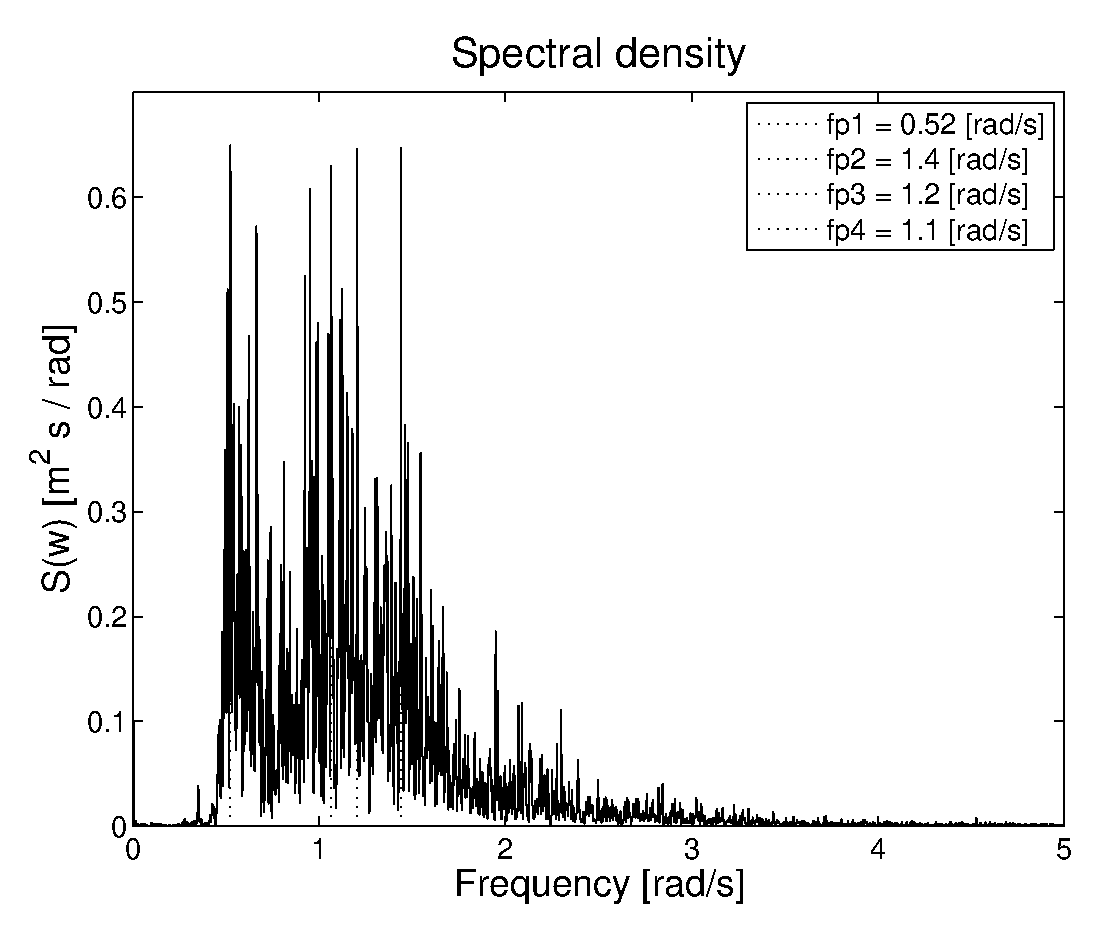
\includegraphics[width=\narrowfigwidth]{fig1_spc}
\vspace{-3mm}
\caption[Non-smoothed spectrum of  {\tt sea.dat}]{
The observed, unsmoothed,  spectrum in the data set {\tt sea.dat}.}
  \label{fig1_spc}
\end{figure}

\begin{cex}{Ex_sea_statistics}
We now calculate the spectrum $\widehat{s}(\omega)$ for the
sea data signal {\tt xx}. \index[xcmds]{{\tt dat2spec}}
{\small\begin{verbatim}
      Lmax = 9500;
      SS = dat2spec(xx,Lmax);
      plotspec(SS); axis([0 5 0 0.7])
\end{verbatim}}\index[xcmds]{{\tt dat2spec2}}

The produced plot, not reproduced in this tutorial, shows the spectrum 
$\widehat{s}(\omega)$ in blue surrounded by 95\% confidence limits, 
in red. These limits can be removed by the command
{\small\begin{verbatim}
      SS = rmfield(SS,'CI')
      plotspec(SS); axis([0 5 0 0.7])
\end{verbatim}}
\noindent giving Figure~\ref{fig1_spc} where we can see that the 
spectrum is extremely
irregular with sharp peaks at many distinct frequencies.
In fact, if we had analysed another section of the sea data we had
found a similar general pattern, but the sharp peaks had been found at
some other frequencies. It must be understood, that the observed
irregularities are random and vary between measurements of the sea
even under almost identical conditions.
This will be further discussed in the following section, where we
introduce smoothing techniques to get a stable spectrum that
represents the ``average randomness'' of the sea state.

Next, the spectral moments will be computed.
{\small\begin{verbatim}
      [mom text] = spec2mom(SS,4)
      [sa sqrt(mom(1))]
\end{verbatim}}\index[xcmds]{{\tt spec2mom}}
The vector {\tt mom} now contains spectral moments $m_0, m_2, m_4$,
which are the variances of the signal and its  first and second
derivative. We can speculate that the variance of
the derivatives is too high because of spurious points.
For example, if there are several points with the same
value, the Gibb's phenomenon leads to high frequencies in the spectrum.
\end{cex}

\subsection{Gaussian processes in spectral domain}
In the previous section we studied the properties of one specific signal
in frequency domain. Assume now that we get a new series of measurements
of a signal, which we are willing to consider as equivalent to the
first one. However, the two series are seldom identical and differ in
some respect that it is natural to regard as purely random.
Obviously it will have a different spectrum $\hat{s}(\omega)$
and the phases will be changed.

A useful mathematical model for such a situation is the random
function (stochastic process) model which will be denoted by $X(t)$.
Then $x(t)$ is seen as particular randomly chosen function.
The simplest model for a stationary signal with a fixed
spectrum $\hat{s}(\omega)$ is
\begin{equation}
X(t)= m + \sum_{i=1}^N \sqrt{\hat{s}_i\, \Delta\omega} \,
\sqrt{2}\cos(\omega_i\,t+\Theta_i),
\label{eqn:sum_with_random_phases}
\end{equation}
where the phases $\Theta_i$ are random variables, independent and
uniformly distributed between $0$ and $2 \pi$.
However, this is not a very realistic model either, since in
practice one often observes a variability in the spectrum amplitudes 
$\hat{s}(\omega)$ between measured functions. Hence, $\hat{s}_i$
should also be modelled to include a certain randomness.

The best way to accomplish this realistic variability  
is to assume that there exists
a deterministic function $S(\omega)$ such that the {\it average value}
of $\widehat{s}(\omega_i)\Delta\omega$ over many observed series
can be approximated by $S(\omega_i)\Delta\omega$. In fact,
in many cases one can model the variability of $\hat{s}_i$ as
$$\hat{s}_i=R_i^2\cdot S(\omega_i)/2,$$
where $R_i$ are independent random factors, all with a Rayleigh distribution,
with probability density function $f_R(r)=r \exp (-r^2/2), r > 0$.
(Observe that the average value of $R_i^2$ is 2.)
This gives the following random function as a model for the series,
\begin{equation}
X(t)= m +
\sum_{i=1}^N \sqrt{S(\omega_i)\, \Delta\omega}\,
R_i\cos(\omega_i\,t+\Theta_i). \label{discretespectrumprocess}
\end{equation}
The process $X(t)$ has many useful properties that can be used for
analysis. In particular, for any fixed $t$, $X(t)$ is normally (Gaussian)
distributed. Then, the probability of any event defined for $X(t)$
can, in principle, be computed when the mean $m$ and the spectral
density $S$ are known.

In sea modelling, the components in the sum defining $X(t)$ can be
interpreted as individual waves. The assumption that $R_i$ and
$\Theta_i$ are independent random variables implies that
the individual waves are independent stationary
Gaussian processes\footnote{A \emph{Gaussian} stochastic process $X(t)$ is
any process such that all linear combinations $\sum a_k X(t_k)$ have a
Gaussian distribution; also derivatives $X'(t)$ and
integrals $\int_a^b X(t)\, \rd t$
are Gaussian.}
with mean zero and covariance function given by
$$
r_i(\tau) = \Delta\omega \, S(\omega_i) \cos(\omega_i\,\tau).
$$
Consequently, the covariance between $X(t)$ and $X(t+\tau)$
is given by
$$
r_X(\tau) = \ex [(X(t)-m)(X(t+\tau)-m)]=\Delta\omega \,\sum_{i=1}^N  S(\omega_i)
\cos(\omega_i\,\tau).
$$
A process like \eqref{discretespectrumprocess}, which is the sum of discrete terms, 
is said to have discrete spectrum. \index[xentr]{spectrum!discrete} Its total energy 
is concentrated to a set of distinct frequencies. 

More generally, for a stationary stochastic process with spectral density
$S(\omega)$, the covariance function $r(\tau)$\index[xentr]{covariance function}  
of the process is defined
by its spectral density function $S(\omega)$,\index[xentr]{spectral density!function} 
also called power spectrum,
\begin{equation}
r(\tau) = \co [X(t), X(t+\tau)] = \int_0^\infty \cos(\omega\tau)
\,S(\omega) \, \rd \omega. \label{spec2cov}
\end{equation}
Since $\va [X(t)] = r_X(0) = \int_0^\infty S(\omega)\, \rd \omega$,
the spectral density represents a continuous distribution of the wave energy
over a continuum of frequencies. The spectrum is continuous. 
\index[xentr]{spectrum!continuous}
\index[xentr]{covariance function!computation from spectrum}

The covariance function and the spectral density form a 
{\it Fourier transform pair}. The spectral density can 
be \index[xentr]{spectrum!computation from covariance function}
computed from the covariance function by the Fourier inversion formula, 
which for continuous-time signals reads,\index[xentr]{Fourier inversion}
\begin{equation}
S(\omega) = \frac{2}{\pi} \int_0^\infty \cos (\omega  \tau) r(\tau)\, \rd \tau.
\label{cov2spec}
\end{equation}

The Gaussian process model is particularly useful in connection
with linear filters. \index[xentr]{linear filter}
If $Y(t)$ is the output of a linear filter
with the Gaussian process $X(t)$ as input,
then  $Y(t)$ is also normally distributed.
Further, the spectrum of $Y(t)$ is related to that of $X(t)$ in
a simple way. If the filter has {\em transfer function}
$H(\omega)$, also called \index[xentr]{transfer function}
{\em frequency function}, \index[xentr]{frequency function}
then the spectrum of $Y(t)$, denoted by $S_Y$,
is given by
$$S_Y(\omega)=|H(\omega)|^2S_X(\omega).$$

For example, the derivative $X'(t)$ is a Gaussian process
with mean zero and spectrum $S_{X'}(\omega)=\omega^2S_X(\omega)$.
The variance of the derivative is equal to the second spectral moment,
$$
\sigma_{X'} ^2=\int S_{X'}(\omega)\, \rd\omega =
\int \omega ^2 S_X(\omega)\, \rd\omega = m_2.
$$

\begin{figure}[tbh]
\centering
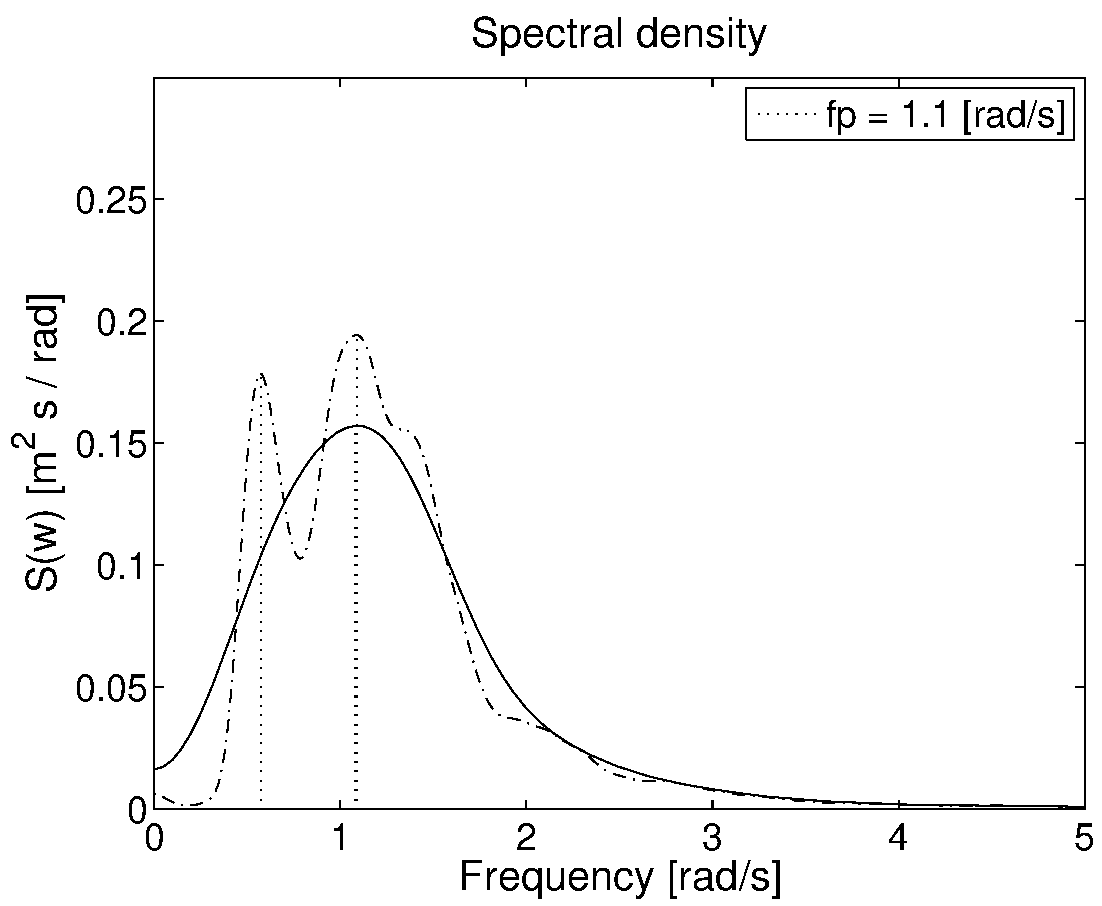
\includegraphics[width=\narrowfigwidth]{fig2_spc}
\vspace{-3mm}
\caption[Spectra  of {\tt sea.dat} with varying degree of smoothing]{
Estimated spectra {\tt SS1, SS2} for the data set {\tt sea.dat}
with varying degree of smoothing; dash-dotted: {\tt Lmax1 = 200}, solid: {\tt Lmax2 = 50}.}
  \label{fig2_spc}
\end{figure}

\begin{cex}{Ex_sea_statistics}
In order to estimate the spectrum of a Gaussian process one needs\index[xentr]{spectrum!estimation of}
  \index[xentr]{spectral density!estimation}
several realizations of the process. Then, one spectrum estimate can be
made for each realization, which are then averaged. However, in many cases
only one realization of the process is available. In such a case
one is often assuming that the spectrum is a smooth function of $\omega$
and one can use this information to improve the estimate. In practice,
it means that one has to use some smoothing techniques.
For the {\tt sea.dat} we shall estimate the spectrum
by means of the \progname{} function
{\tt dat2spec}\index[xcmds]{{\tt dat2spec}}
with a second parameter defining the degree of smoothing.\label{page:SS1}
{\small\begin{verbatim}
      Lmax1 = 200; 
      Lmax2 = 50;
      SS1 = dat2spec(xx,Lmax1);
      SS2 = dat2spec(xx,Lmax2);
      plotspec(SS1,[],'-.'), hold on
      plotspec(SS2), hold off
\end{verbatim}}
\noindent In Figure~\ref{fig2_spc}
we see that with decreasing second input the spectrum estimate becomes 
smoother, and that in the end it becomes unimodal.

An obvious question after this exercise is the following: Which of the two estimates in 
Figure~\ref{fig2_spc} is more correct, in the sense that it best reflects 
important wave characteristics? Since the correlation structure is a very 
important characteristic, we check which spectrum can best reproduce the 
covariance function of the data {\tt xx}. 

The following
code in \progname{} will compute the covariance for the bimodal spectral
density {\tt S1}\index[xcmds]{{\tt covplot}}\index[xcmds]{{\tt spec2cov}}\index[xcmds]{{\tt dat2cov}}
and compare it with the estimated covariance in the signal {\tt xx}.
{\small\begin{verbatim}
      Lmax = 80;
      R1 = spec2cov(SS1,1);
      Rest = dat2cov(xx,Lmax);
      covplot(R1,Lmax,[],'.'), hold on
      covplot(Rest), hold off
\end{verbatim}}
\noindent With the unimodal spectrum {\tt SS2} instead of {\tt SS1} we also compute the 
covariance function {\tt R2 = spec2cov(SS2,1)} and plot it together with {\tt Rest}.  

We can see in Figure~\ref{fig4_s2c}(a)
that the covariance function corresponding to the spectral density {\tt SS2}
differs significantly from the one estimated directly from data.
The covariance corresponding to {\tt SS1} agrees much
better with the estimated covariance function, as seen in Figure~\ref{fig4_s2c}(b). 
Our conclusion is that the bimodal spectrum in Figure~\ref{fig2_spc} is a better 
model for the data {\tt sea.dat} than the unimodal one. 
~ \end{cex}

\begin{figure}
\subfigure[]{%
\label{fig4_s2ca}
\begin{minipage}[b]{0.49\textwidth}%
\centering 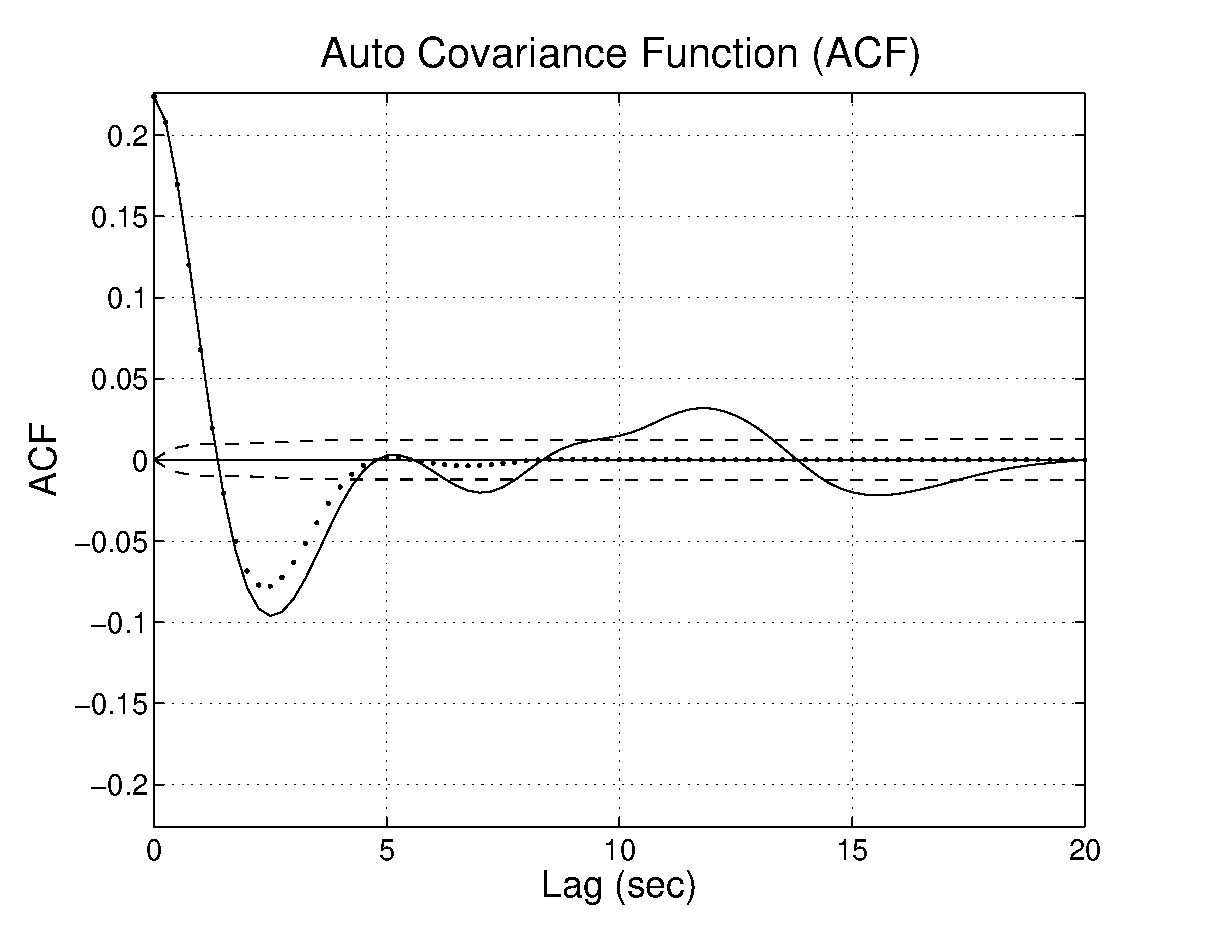
\includegraphics[width=\defwidth]{fig4_s2cb}
\end{minipage}}%
\hfill
\subfigure[]{%
\label{fig4_s2cb}
\begin{minipage}[b]{0.49\textwidth}%
\centering 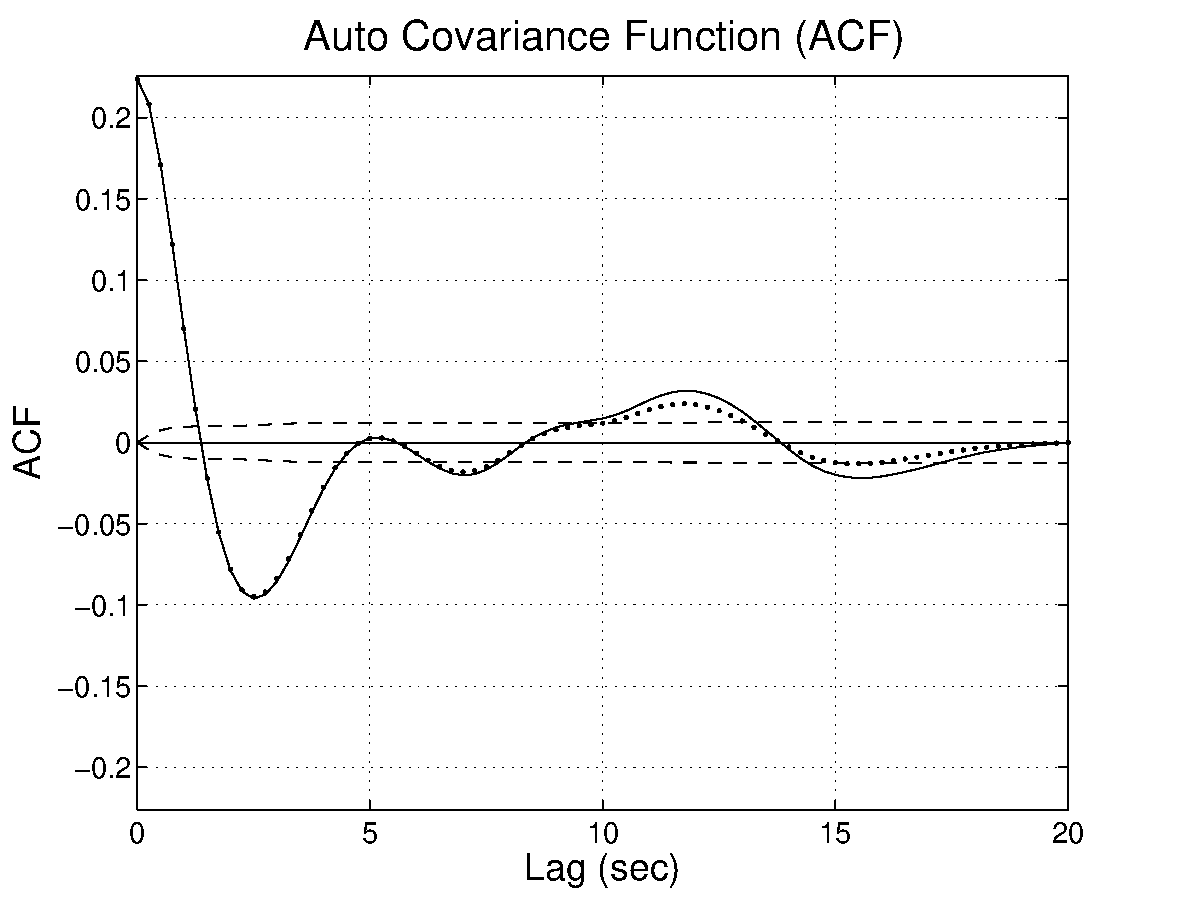
\includegraphics[width=\defwidth]{fig4_s2ca}
\end{minipage}}
\vspace{-3mm}
\caption[ACF computed from spectra of
{\tt sea.dat} with smoothing]{
The covariance function estimated in the data set {\tt sea.dat}, solid line,
compared to the theoretically computed covariance functions for the spectral
densities {\tt SS2} in (a) and {\tt SS1} in (b).
}
  \label{fig4_s2c}
\end{figure}

Observe that the \progname{} function {\tt spec2cov} can be used to compute
a covariance structure which can contain covariances both in time and in
space as well as that of the derivatives.
The input can be any spectrum structure, e.g.\ wavenumber spectrum,
directional spectrum or encountered directional spectrum;
type {\tt help spec2cov} for detailed information.

\subsection{Crossing intensity -- Rice's formula}
\label{subsec:crossing_intensity}
\index[xentr]{Rice's formula}
The Gaussian process is a sum (or in fact an integral) of cosine terms with amplitudes defined
by the spectrum, and the instantaneous value $X(t)$ has a normal distribution
with mean $0$ and variance $\sigma^2 = \int S(\omega)\, \rd \omega$. 
The spectral density $S(\omega)$ determines the relative importance of 
components with different frequencies. 

In wave analysis and fatigue applications there is another quantity that
plays a central role, namely the {\em upcrossing intensity} $\mu(u)$,
which yields the average number, per time or space unit,
of upcrossings of the level $u$. It
contains important information on the fatigue properties of a
load signal and also of the wave character of a random wave.\footnote{%
The general expression for the upcrossing intensity for a stationary process
 is
$\mu(u)=\int_{z=0}^\infty z\, f_{X(0),X'(0)}(u,z)\, \rd z$, where
$f_{X(0),X'(0)}(u,z)$ is a joint probability density function.}

For a Gaussian process the crossing intensity
is given by the celebrated {\it Rice's formula},
\index[xentr]{Rice's formula}
\begin{equation}
\mu(u)=f_0\exp\left\{-\frac{(u-m)^2}{2\sigma^2}\right\}.\label{eq:rice}
\end{equation}
Using spectral moments we have that $\sigma^2=m_0$ while
$f_0=\frac{1}{2\pi}\sqrt{\frac{m_2}{m_0}}$ is the mean frequency.
\index[xentr]{mean frequency}

\subsection{Transformed Gaussian models}\label{ss:transformedGaussianmodels}
\index[xentr]{transformed Gaussian models|(}

The standard assumptions for a sea state under stationary conditions are
that $X(t)$ is a stationary and ergodic stochastic process with
mean $\ex[X(t)]$ assumed to be zero, and with a spectral density
$S(\omega)$. The knowledge of which kind of spectral densities
$S(\omega)$ are suitable to describe different sea state data is well
established from experimental studies.

Real data $x(t)$ seldom perfectly support the Gaussian assumption for
the process $X(t)$. But since the Gaussian case is well understood
and there are approximative methods to obtain wave characteristics
from the spectral density $S(\omega)$ for Gaussian processes,
one often looks for a model of the sea state in the
class of Gaussian processes. Furthermore, in previous work,
\cite{RychlikEtal1997Modelling},
%,RyLJ97} %Rychlik, Leadbetter and Johannesson 1997
we have found that for many sea wave data, even such that are clearly
non-Gaussian, the wavelength and amplitude densities can be very
accurately  approximated using the Gaussian process model.

However, the Gaussian model can lead to less satisfactory results
when it comes to the distribution of crest heights or joint densities
of troughs and crests. In that case we found in
\cite{RychlikEtal1997Modelling}
that a simple transformed Gaussian process used to model $x(t)$ gave
good approximations for those densities.

Consequently, in \progname{} we shall model $x(t)$ by a process $X(t)$ which is a
function of a single Gaussian process $\widetilde X (t)$, i.e.\
\begin{equation}\label{eq:trprocess}
X(t)=G(\widetilde X(t)),
\end{equation}
where $G(\cdot)$ is a continuously differentiable function with
positive derivative.  We shall denote the spectrum of $X$ by $S$,
and the spectrum of $\widetilde X (t)$ by $\widetilde S$.
The transformation $G$ performs the appropriate non-linear
translation and scaling so that $\widetilde X(t)$ is always normalized to
have mean zero and variance one, i.e.\ the first spectral moment of
$\widetilde S$ is one.

Note that once the distributions of crests, troughs, amplitudes or
wavelengths in a Gaussian process $\widetilde X (t)$ are computed, then
the corresponding wave distributions in $X(t)$ are obtained by a simple
variable transformation involving only the inverse of $G$, which we
shall denote by $g$. Actually we shall use the function $g$ to define
the transformation instead of $G$, and use the relation $\widetilde x
(t) = g(x(t))$ between the real sea data $x(t)$ and the transformed
data $\widetilde x (t)$.
If the model in Eq.~(\ref{eq:trprocess}) is correct, then
$\widetilde x(t)$ should be a sample function of a process with
Gaussian marginal distributions.
%Obviously, a Gaussian model is
%obtained by using a linear function $g(y)=ay + b$, where $a, b$ are
%constants.

There are several different ways to proceed when selecting a transformation.
The simplest alternative is to estimate the function
$g$ directly from data by some parametric or non-parametric techniques. A more
physically motivated procedure is to use some of the parametric functions
proposed in the literature, based on approximations of non-linear wave
theory.  The following options are programmed in the
toolbox:
{\small\begin{verbatim}
      dat2tr    - non-parametric transformation g proposed by Rychlik,
      hermitetr - transformation g proposed by Winterstein,
      ochitr    - transformation g proposed by Ochi et al.
\end{verbatim}}
\index[xentr]{transformed Gaussian models!Winterstein}
\index[xentr]{transformed Gaussian models!Ochi et al.}
\index[xentr]{transformed Gaussian models!Rychlik}
\index[xentr]{transformed Gaussian models!nonparametric}
\index[xcmds]{{\tt hermitetr}}
\index[xcmds]{{\tt ochitr}}
\index[xcmds]{{\tt dat2tr}}

The transformation proposed by by Ochi et al.,
\cite{OchiAndAhn1994Probability},
is a monotonic exponential function, while Winterstein's model,
\cite{Winterstein1988Nonlinear}, is a
monotonic cubic Hermite polynomial. Both transformations use higher moments
of $X(t)$ to compute $g$. Information about the moments of the process
can be obtained by site specific data, laboratory measurements or from
physical considerations. Rychlik's non-parametric method is based on
the crossing intensity $\mu(u)$; see \cite{RychlikEtal1997Modelling}.
Martinsen and Winterstein, \cite{MarthinsenAndWinterstein1992Skewness},
derived an expression for the
skewness and kurtosis for narrow banded Stokes waves to the leading order
and used these to define the transformation.
The skewness and kurtosis (excess) of this model can also be estimated from
data by the \progname{} functions {\tt skew}
\index[xcmds]{{\tt skew}}
and {\tt kurt}\index[xcmds]{{\tt kurt}}.

\begin{cex}{Ex_sea_statistics}
We begin with computations of skewness and kurtosis
for the data set {\tt xx}. The commands
{\small\begin{verbatim}
      rho3 = skew(xx(:,2))
      rho4 = kurt(xx(:,2))
\end{verbatim}}
\noindent
give the values {\tt rho3 = 0.25} and {\tt  rho4 = 3.17},
respectively, compared to {\tt rho3 = 0} and  {\tt rho4 = 3}
for Gaussian waves. We can compute the same model for
the spectrum $\tilde S$ using the second order wave approximation
proposed by Winterstein. His approximation gives suitable
values for skewness and kurtosis
{\small\begin{verbatim}
      [sk, ku] = spec2skew(S1);
\end{verbatim}}\index[xcmds]{{\tt spec2skew}}

Here we shall use Winterstein's Hermite transformation
and denote it by {\tt gh},
and compare it with the linear transformation, denoted by {\tt g}, that
only has the effect to standardize the signal, assuming it is already Gaussian,
{\small\begin{verbatim}
      gh = hermitetr([],[sa sk ku me]);
      g  = gh; g(:,2)=g(:,1)/sa;
      trplot(g)
\end{verbatim}}\index[xcmds]{{\tt hermitetr}}
\noindent These commands will result in two two-column matrices,
{\tt g, gh}, with equally spaced $y$-values in the first column
and the values of $g(y)$ in the second column.

Since we have data we may estimate the transformation directly by the method
proposed by Rychlik et al., in \cite{RychlikEtal1997Modelling}:
{\small\begin{verbatim}
      [glc test0 cmax irr gemp] = dat2tr(xx,[],'plotflag',1);
      hold on
      plot(glc(:,1),glc(:,2),'b-')
      plot(gh(:,1),gh(:,2),'b-.'), hold off
\end{verbatim}}\index[xcmds]{{\tt dat2tr}}
\noindent The same transformation can be obtained from data 
and the crossing intensity by use of the \progname{} functions  
{\tt dat2lc} followed by 
{\tt lc2tr}\index[xcmds]{{\tt lc2tr}}\index[xcmds]{{\tt dat2lc}}.

\begin{figure}[thb]
\centering
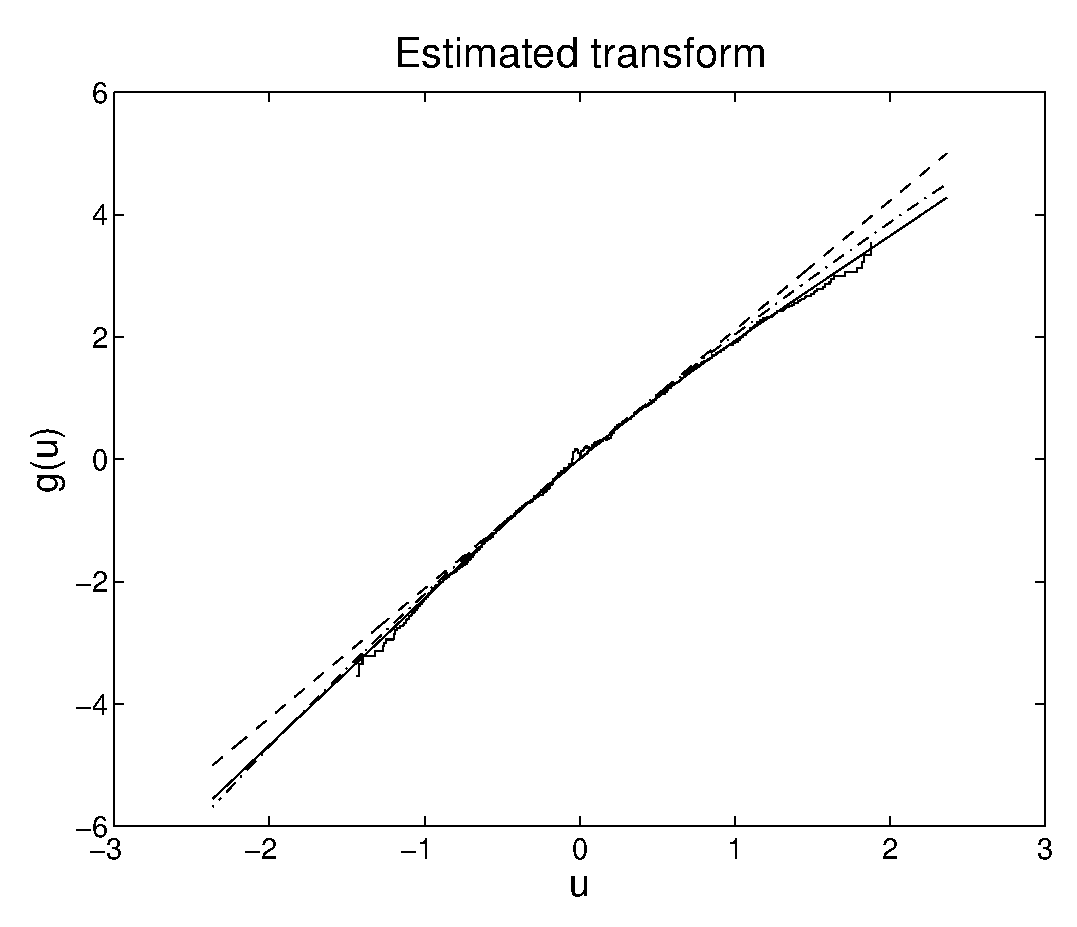
\includegraphics[width=\narrowfigwidth]{fig4_tr}
\vspace{-3mm}
\caption[Comparison of data transformations]{%
Comparisons of the three transformations $g$,
straight line is the Gaussian model,
dash dotted line the Hermite transformation {\tt gh} and solid line the
Rychlik method {\tt glc}.}
  \label{fig4_tr}
\end{figure}

In Figure~\ref{fig4_tr} we compare the three transformations,
the straight line is the Gaussian linear model, the dash dotted
line is the Hermite transformation based on higher moments of the
response computed from the spectrum and the solid line is the direct
transformation estimated from crossing intensity.
(The unsmoothed line shows the estimation of
the direct transformation from unsmoothed crossing intensity).
We can see that the transformation derived from crossings will give
the highest crest heights. It can be proved that asymptotically
the transformation based on crossings intensity gives the
correct density of crest heights.

The transformations indicate that data {\tt xx} has a light
lower tail and heavy
upper tail compared to a Gaussian model.
This is also consistent with  second order wave theory, where the crests
are higher and the troughs shallower compared to Gaussian waves.
Now the question is whether this difference is significant
compared to the natural statistical variability due to finite length
of the time series.

\begin{figure}[t]
\centering
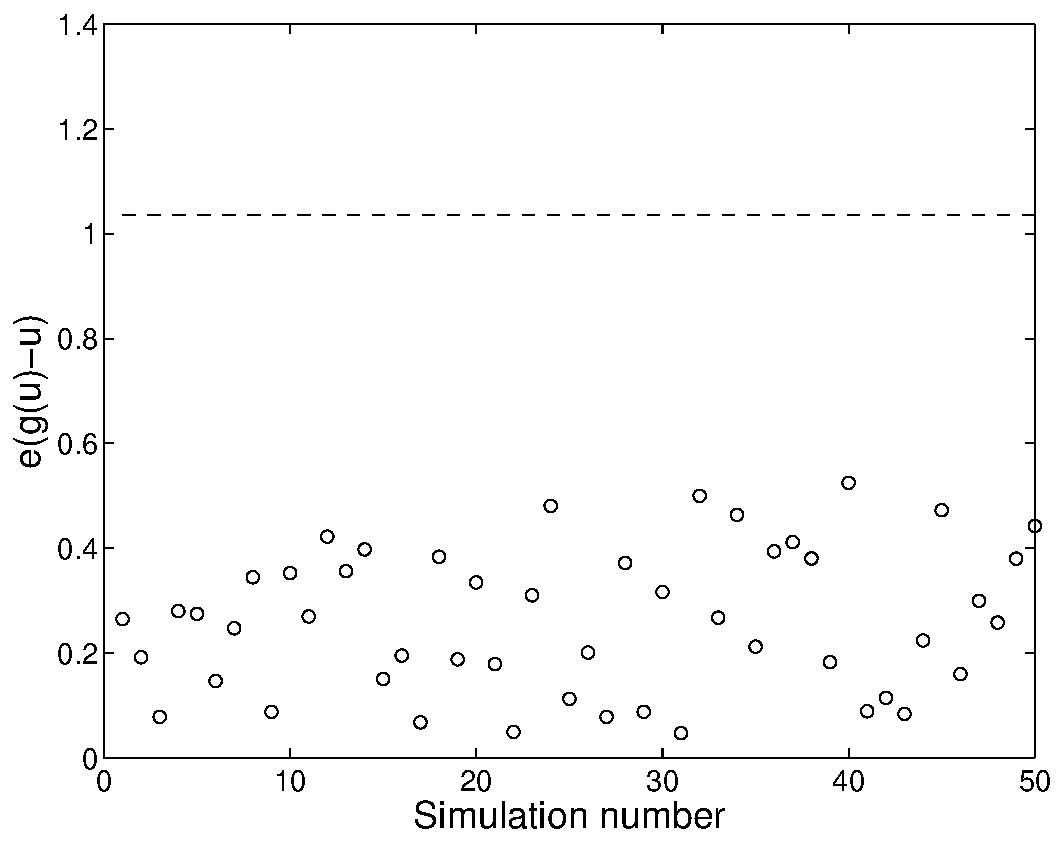
\includegraphics[width=\narrowfigwidth]{figure_Ch2_8}
\vspace{-3mm}
\caption[Simulation technique to test if a stochastic process is Gaussian]{
The simulated 50 values of the {\tt test} variable for
the Gaussian process with spectrum {\tt S1} compared with the
observed value (dashed line).}
  \label{fig2-3}
\end{figure}

To determine the degree of departure from Gaussianity,
we can compare an indicator of non-Gaussianity {\tt test0}
obtained from Monte Carlo simulation. The value
of {\tt test0} is a measure of how munch the transformation {\tt g}
deviates from a straight line.

The significance test is done by simulating 50 independent samples
of {\tt test0} from a true Gaussian process with the same spectral
density and length as the original data. This is accomplished
by the \progname{} program \verb+testgaussian+\index[xcmds]{{\tt testgaussian}}.
The output from the program is
a plot of the ratio \verb+test1+ between the simulated (Gaussian)
{\tt test0}-values and the sample {\tt test0}, that was calculated in the previous call to 
{\tt dat2tr}:
{\small\begin{verbatim}
      N = length(xx);
      test1 = testgaussian(S1,[N,50],test0);
\end{verbatim}}
\noindent
The program gives a plot of simulated {\tt test} values, see
Figure~\ref{fig2-3}. As we see from the figure none of the
simulated values of \verb+test1+ is above 1.00. Thus the data
significantly departs from a Gaussian distribution;
see \cite{RychlikEtal1997Modelling} for more detailed discussion
of the testing procedure and the estimation of the transformation
{\tt g} from the crossing intensity.

We finish the tests for Gaussianity of the data by a more classical
approach and simply plot the data on normal probability paper.
Then $N$ independent observations of identically distributed Gaussian
variables form a straight line in a normalplot.
Now, for a time series the data is clearly not
independent. However, if the process is ergodic then
the data forms a straight line as $N$ tends to infinity.

The command \index[xcmds]{{\tt plotnorm}}
{\small\begin{verbatim}
      plotnorm(xx(:,2))
\end{verbatim}}
\noindent produces Figure~\ref{fig2-4}.
As we can see the normal probability plot is slightly curved
indicating that the underlying distribution has a heavy
upper tail and a light lower tail.
\end{cex}
\begin{figure}[t]
\centering
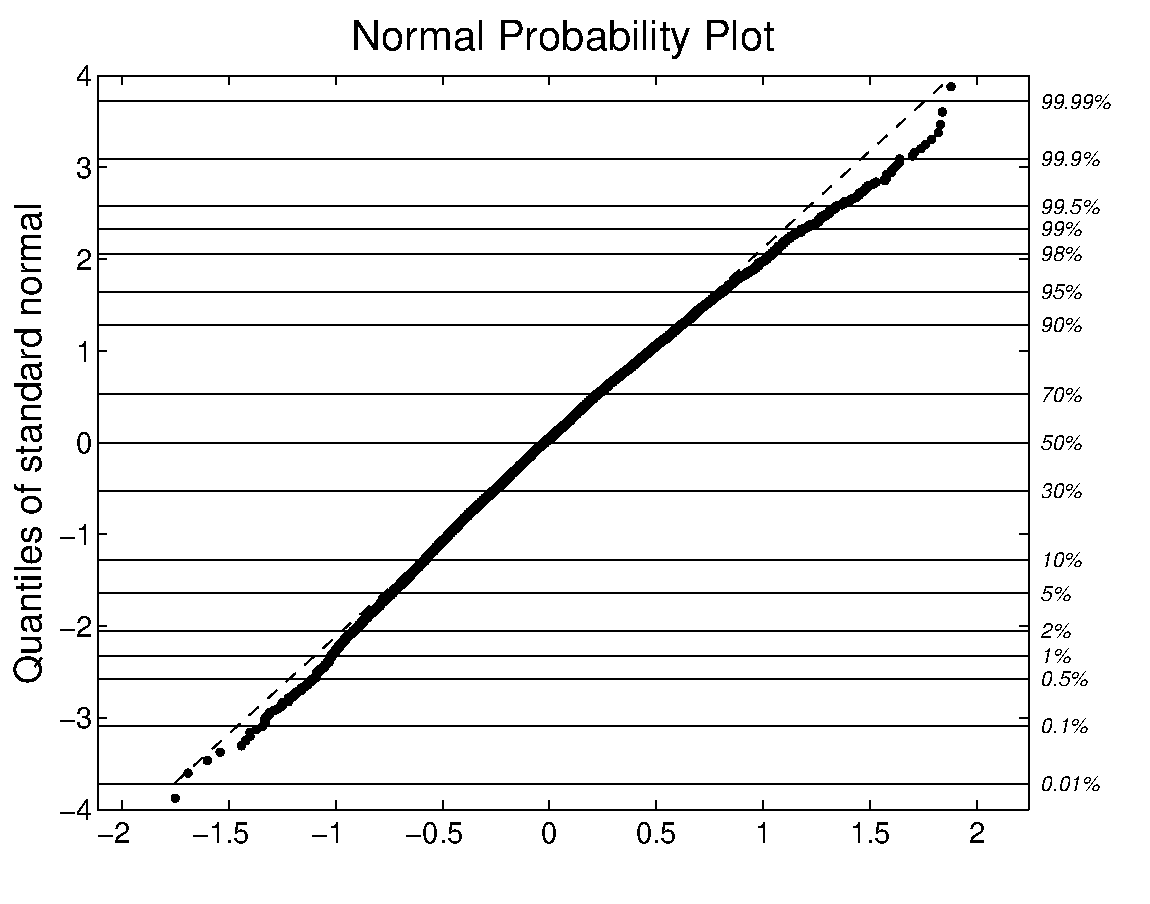
\includegraphics[width=\narrowfigwidth]{figure_Ch2_2}
\vspace{-3mm}
  \caption[Normal probability plot]{The data {\tt sea.dat} on
   normal probability plot.}
  \label{fig2-4}
\end{figure}

\index[xentr]{transformed Gaussian models|)}
\subsection{Spectral densities of sea data}
\index[xentr]{spectrum!of sea data|(}

The knowledge of which kind of spectral density $S(\omega)$ is suitable
to describe sea state data is well established from experimental
studies. One often uses some parametric form of spectral density
functions, e.g.\ a {\sc Jonswap}-spectrum. \index[xentr]{Jonswap spectrum}
This formula is programmed in a \progname{}
function \index[xentr]{spectrum!Jonswap}
{\tt jonswap}, which evaluates the spectral density $S(\omega)$
with specified wave characteristics. There are several other
programmed spectral densities in \progname{} to allow for bimodal and
finite water depth spectra. The list includes the following spectra:
{\small\begin{verbatim}
      jonswap       - JONSWAP spectral density
      wallop        - Wallop spectral density
      ochihubble    - Bimodal Ochi-Hubble spectral density
      torsethaugen  - Bimodal (swell + wind) spectral density
      bretschneider - Bretschneider (Pierson-Moskowitz)
                      spectral density
      mccormick     - McCormick spectral density
      tmaspec       - JONSWAP spectral density
                      for finite water depth
\end{verbatim}}
\index[xcmds]{{\tt jonswap}}\index[xcmds]{{\tt wallop}}
\index[xcmds]{{\tt ochihubble}}\index[xcmds]{{\tt torsethaugen}}
\index[xcmds]{{\tt bretschneider}}\index[xcmds]{{\tt mccormick}}
\index[xcmds]{{\tt tmaspec}}\index[xcmds]{{\tt spec}}
\index[xcmds]{{\tt spreading}}
\progname{} also contains some different spreading functions;
use the help function on {\tt spec} and {\tt spreading}
for more detailed information.

The spectrum of the sea can be given in many different formats,
that are interconnected by the dispersion
relation\footnote{The dispersion relation between frequency
$\omega$ and wavenumber $\kappa$ on finite water depth $h$, reads
$\omega^2=g \kappa \tanh h\kappa$, where $g$ is the acceleration of gravity.}.
The spectrum can be given using
frequencies, angular frequencies or wavenumbers, and it
can also be directional.

A related spectrum is the encountered spectrum for a moving vessel. The
transformations between the different types of spectra
are defined by means of integrals and variable change defined by the
dispersion relation
and the Doppler shift of individual waves.
The function {\tt spec2spec}\index[xcmds]{{\tt spec2spec}}
makes all these transformations easily
accessible for the user. (Actually many programs perform
the appropriate transformations internally whenever it is necessary
and for example one can compute the density of wave-length,
which is a quantity in space domain, from an
input that is the directional frequency spectrum, which is related to the
time domain.)

\begin{figure}[tbh]
\centering
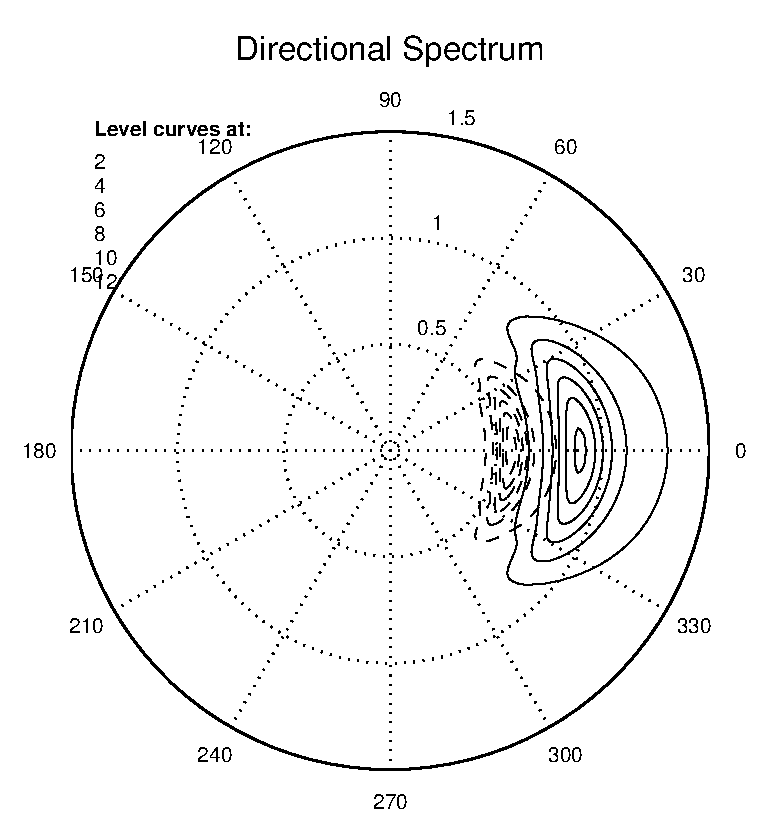
\includegraphics[width=\narrowfigwidth]{figure_spec_enc}
\vspace{-3mm}
\caption[Example of directional spectra]{
Directional spectrum {\tt SJd} of {\sc Jonswap} sea (dashed line)
 compared with the encountered directional spectrum {\tt SJe} for heading sea,
 speed 10 [m/s] (solid line).}
  \label{fig4-5}
\end{figure}

\begin{rtex}{Ex_sea_spectra}{Different forms of spectra}
In this example we have chosen a {\sc Jonswap} spectrum with parameters
defined by significant wave height {\tt Hm0 = 7[m]} and peak period
{\tt Tp = 11[s]}. This spectrum describes the measurements of sea
level at a fixed point (buoy).
{\small\begin{verbatim}
      Hm0 = 7; Tp = 11;
      SJ = jonswap([],[Hm0 Tp]);
      SJ.note
\end{verbatim}} \index[xcmds]{{\tt jonswap}}\index[xentr]{spectrum!Jonswap}

In order to include the space dimension, i.e.\ the direction in which
the waves propagate, we compute a directional spectrum by
adding spreading; see dashed curves in Figure~\ref{fig4-5}.
{\small\begin{verbatim}
      D = spreading(101,'cos2s',0,[],SJ.w,1)
      SJd = mkdspec(SJ,D)  % Directional spectrum
\end{verbatim}}

Next, we consider a vessel moving with
speed {\tt 10[m/s]} against the waves. The sea measured
from the vessel will have a different directional spectrum,
called the encountered  directional spectrum. \index[xentr]{encountered directional spectrum}
The following code will compute the encountered
directional spectrum and plot it on top of
the original spectrum. The result is shown as
the solid curves in Figure~\ref{fig4-5}.
{\small\begin{verbatim}
      SJe = spec2spec(SJd,'encdir',0,10);  % Encountered dir spectrum
      plotspec(SJe), hold on
      plotspec(SJd,1,'--'), hold off
\end{verbatim}} \index[xentr]{spectrum!encountered}
\index[xentr]{spectrum!directional}

Obviously, the periods of waves in the directional sea are defined by
the {\sc Jonswap} spectrum
(in a linear wave model spreading does not affect the sea level at a fixed point),
but the encountered periods will be shorter with heading seas.
This can be seen by comparing the original {\sc Jonswap} spectrum
\verb+SJ+ with the following two point spectra. 
{\small\begin{verbatim}
      SJd1 = spec2spec(SJd,'freq'); % Point spectrum from dir spectrum
      SJd2 = spec2spec(SJe,'enc');  % Point encountered spectrum at ship
      plotspec(SJ), hold on
      plotspec(SJd1,1,'.'),
      plotspec(SJd2), hold off
\end{verbatim}}
\noindent We can see in Figure~\ref{fig4-4}(a) that the spectra
{\tt SJ} and {\tt SJd1} are identical (in numerical sense),
while spectrum {\tt SJd2} contains more energy at higher frequencies.

A similar question is how much the
wave length differs between a longcrested {\sc Jonswap} sea
and a {\sc Jonswap} sea with spreading. The answer lies in 
the {\it wavenumber spectrum}\index[xentr]{spectrum!wavenumber}
that measures how the wave enegy is distributed over different 
wavenumbers, i.e.\ radians (or cycles)  \index[xentr]{wavenumber}
per unit length along a specified direction, usually the main wave direction. 

The wavenumber spectra along the main wave direction 
can be computed by the following  code,
the result of which is shown in Figure~\ref{fig4-4}(b).
{\small\begin{verbatim}
      SJk = spec2spec(SJ,'k1d')  % Unidirectional waves
      SJkd = spec2spec(SJd,'k1d')  % Waves with directional spreading 
      plotspec(SJk), hold on
      plotspec(SJkd,1,'--'), hold off
\end{verbatim}}
\noindent We see how the spreading of energy away from the main direction 
makes observed waves longer. The total energy is of course the same but 
shifted to lower wavenumbers.   

\begin{figure}[tbh]
\subfigure[]{%
\begin{minipage}[b]{0.5\textwidth}%
    \centering   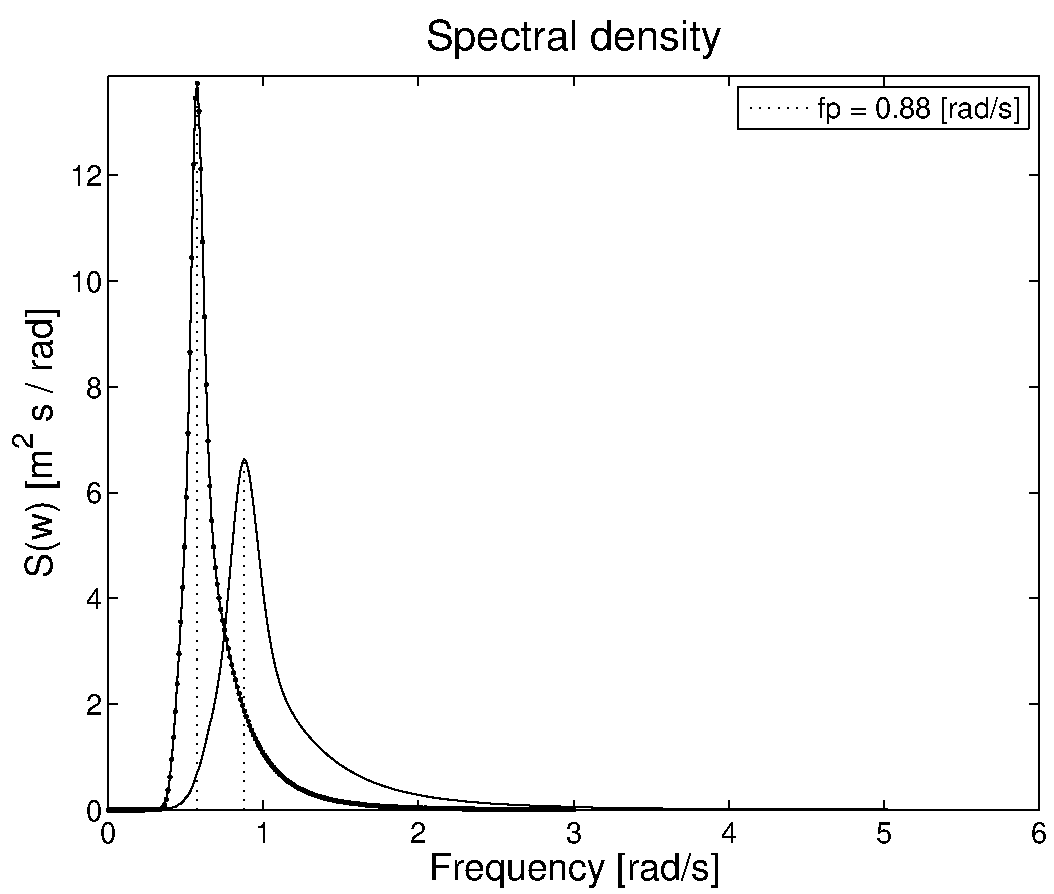
\includegraphics[width=\defwidth]{fig4_Je} %
  \end{minipage}}%
\hfill
\subfigure[]{%
\begin{minipage}[b]{0.5\textwidth}%
    \centering   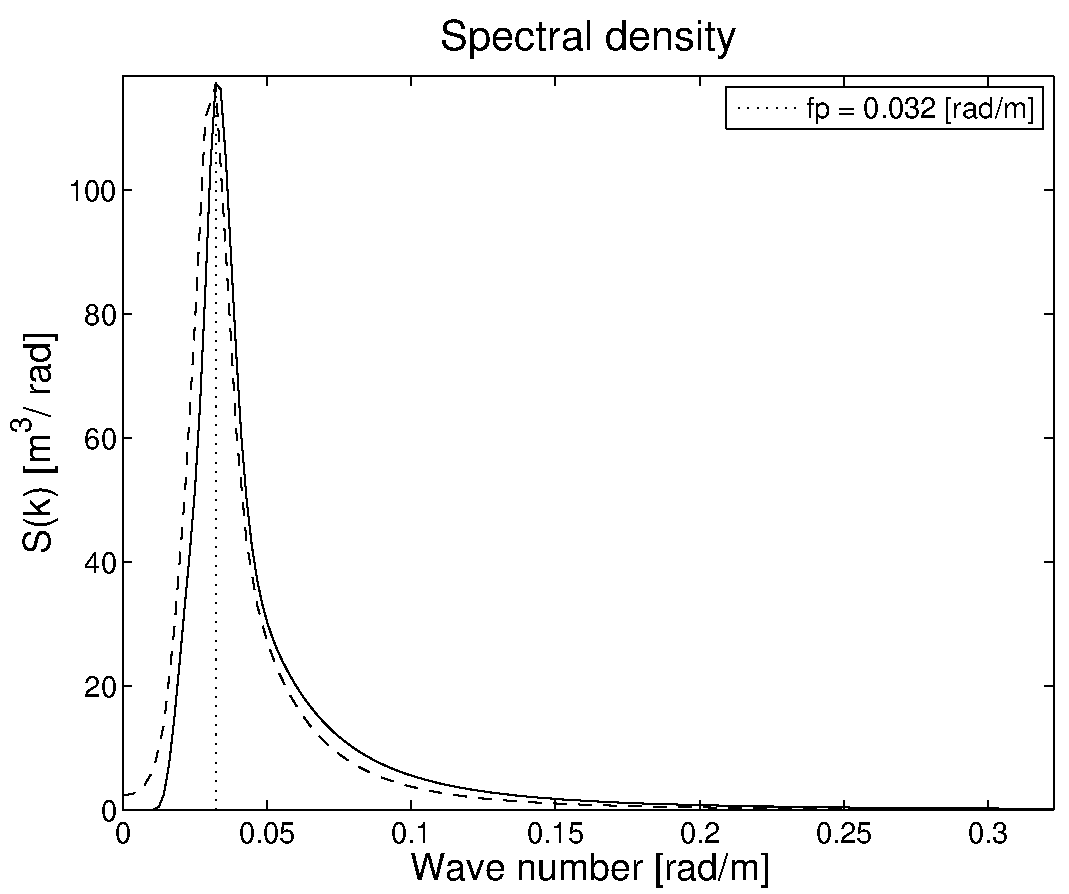
\includegraphics[width=\defwidth]{figure_spec_k1d} %
  \end{minipage}}%
\vspace{-3mm}
\caption[Comparing different forms of spectra]{
 (a) Frequency {\sc Jonswap} spectrum {\tt SJ} and point spectrum 	
 {\tt SJd1} compared with encountered point 
 spectrum {\tt SJd2} for heading sea speed 10 [m/s] (solid line).
(b) Wavenumber spectrum {\tt SJk} for longcrested {\sc Jonswap} sea
(solid line) compared with wavenumber spectrum {\tt SJkd} 
for {\sc Jonswap} with spreading (dashed).
}
  \label{fig4-4}
\end{figure}

Finally, we shall show how the {\sc Jonswap} spectrum
can be corrected  for a finite depth, see \cite{BuowsEtal1985Similarity} for a 
theoretical and empirical study.
The \progname{} function {\tt phi1} computes the frequency dependent 
reduction of the spectrum for waters of finite depth, here 20 meters.
{\small\begin{verbatim}
      plotspec(SJ,1,'--'), hold on
      SJ20 = SJ;
      SJ20.S = SJ20.S.*phi1(SJ20.w,20); % Finite depth correction
      SJ20.h = 20;
      plotspec(SJ20),  hold off
\end{verbatim}} \index[xcmds]{{\tt phi1}}
\noindent The resulting spectra are shown in Figure~\ref{fig4-1}.
\end{rtex}
\begin{figure}[hbt]
\centering
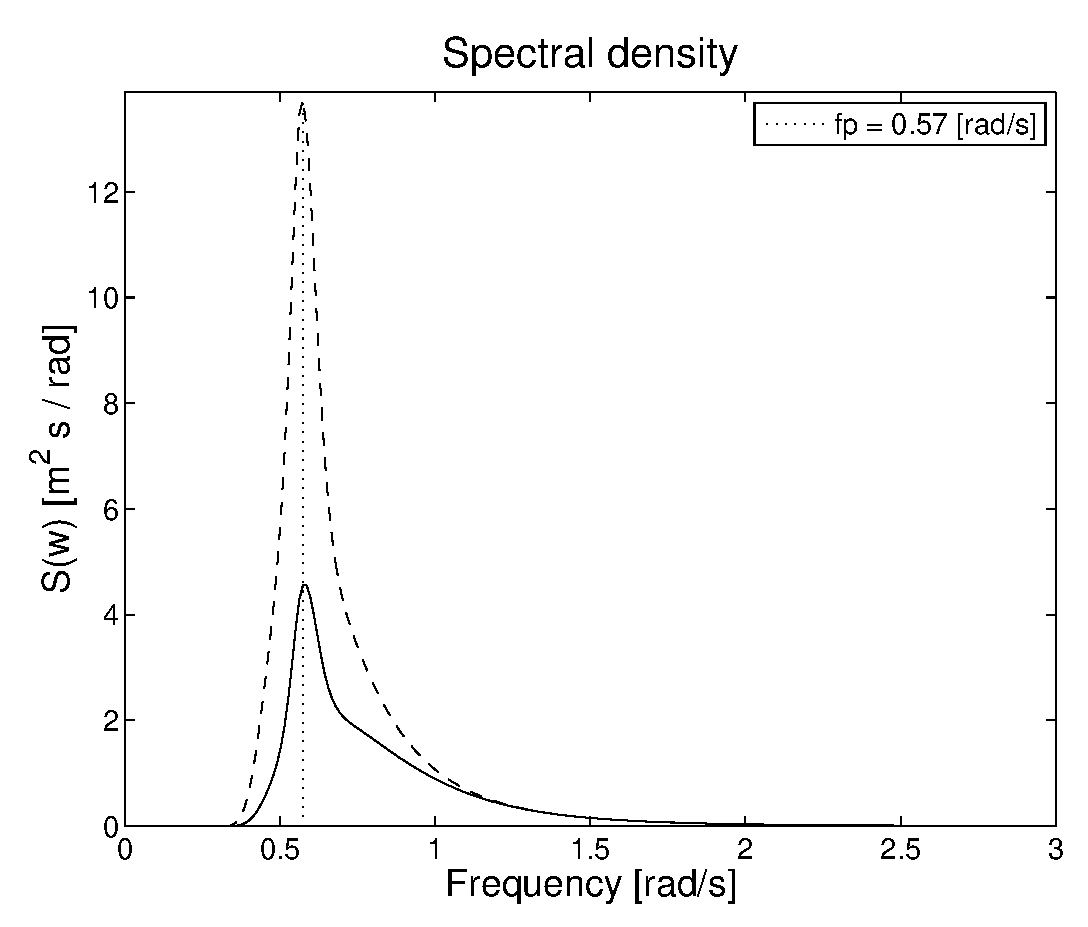
\includegraphics[width=\narrowfigwidth]{figure_spec}
\vspace{-3mm}
  \caption[{\sc Jonswap} spectrum compared
with spectrum on finite depth]{
Standard {\sc Jonswap} spectrum {\tt SJ} (dashed line)
compared with the spectrum {\tt SJ20} on finite depth
of 20 [m] (solid line)
}
  \label{fig4-1}
\end{figure}

\index[xentr]{spectrum!of sea data|)}
\index[xentr]{spectrum!finite depth}

\section{Simulation of transformed Gaussian
  process}\label{sec:simulationofGaussian}
\index[xentr]{transformed Gaussian models|(}
\index[xentr]{transformed Gaussian models!simulation of|(}
\index[xentr]{simulation!of transformed Gaussian process|(}

In this section we shall present some of the programs that can be used to simulate 
%random signals, loads and waves; type {\tt help simtools} for a list.
%We shall be mostly concerned with simulation of the 
the transformed Gaussian model for sea $X(t)=G(\widetilde X(t))$. 
In \progname{} there are several other programs to simulate random functions
or surfaces, both Gaussian and non-Gaussian; use {\tt help simtools}. 
We give examples of some of these functions in Section~\ref{s:2.4}.  

The first important case is when we wish to reproduce random versions
of the measured signal $x(t)$. Using {\tt dat2tr}\index[xcmds]{{\tt dat2tr}}
one first
estimates the transformation {\tt g}. Next, using a function
{\tt dat2gaus}\index[xcmds]{{\tt dat2gaus}}
one can compute $\tilde x(t)=g(x(t))$, which we assume is a realization
of a Gaussian process. From $\tilde x$ we can then estimate
the spectrum $\tilde S(\omega)$ by means of the function
{\tt dat2spec}. The spectrum $\tilde S(\omega)$ and the transformation
$g$ will uniquely define the transformed Gaussian model. A random
function that models the measured signal can then be obtained using the
simulation program {\tt spec2sdat}\index[xcmds]{{\tt spec2sdat}}, 
which includes the desired transformation.
In the following example we shall illustrate
this approach on the data set {\tt sea.dat}.

Before we can start to simulate we need to put the transformation into the
spectrum data structure, which is a \ML{} structure variable; 
see Section~\ref{sec:datastructures}, page~\pageref{sec:datastructures}. 
Since \progname{} is based on transformed Gaussian
processes the entire process structure is defined by the spectrum and
the transformation together. Therefore the transformation has been
incorporated, as part of a model, into the spectrum structure, and is
passed to other \progname{} programs via the spectrum.
If no transformation is given then the process is Gaussian.

Observe that the possibly nonzero mean {\tt m} for the model is
included in the transformation. The change of mean by for example 0.5~[m]
is simply accomplished by modifying the transformation 
by the command {\tt g(:,2) = g(:,2)+0.5;}
Consequently the spectrum structure completely defines the model.

\bigskip
\noindent
{\bf\sc Important note 1:} \label{ImpNote_1} When the simulation routine \verb+spec2sdat+
is called with a spectrum argument that contains a scale changing
transformation \verb+spectrum.tr+, then it is
assumed that the input spectrum is standardized
with spectral moment $m_0=1$, i.e.\ unit variance. The correct
standard deviation
for the output should normally be  obtained via the transformation
\verb+spectrum.tr+. If you happen to use a transformation
{\it together with} an input spectrum that does not have unit
variance, then you get the double scale effect, both from the
transformation and via
the standard deviation from the spectrum. It is only the routine
\verb+spec2sdat+ that works in this way. All other routines, in
particular those which calculate cycle distributions, perform an
internal normalization of the spectrum before the calculation, and
then transforms back to the original scale at the end.

\bigskip
\noindent
{\bf\sc Important note 2:} When you run the simulation examples 
with different time horizon and time step you may experience a
warning

\centerline{
 {\tt 'Spectrum matrix is very large'}.
 }
 
 \noindent
This is a warning from the \wf{} routine {\tt specinterp}, which is used 
internally to adapt the spectrum to the correct Nyquist frequency 
and frequency resolution. You can turn off the warning by commenting 
out three lines in {\tt specinterp} in the {\tt spec} 
module.\index[xcmds]{{\tt specinterp}}

\begin{rtex}{Ex_sea_simulation}{Simulation of a random sea}
\index[xentr]{simulation!of random sea}
In Example~\ref{Ex_sea_statistics} on page~\pageref{page:spurious}
we have shown that the
data set {\tt xx = sea.dat} contains a considerable amount of
spurious points that we would like to omit or censor.

The program \verb+reconstruct+\index[xcmds]{{\tt reconstruct}}
replaces the spurious data by
synthetic data. The new data points are obtained by simulation of 
a conditional Gaussian vector, based on the remaining data, taking the 
fitted transformed Gaussian process model into account; 
see
\cite{BrodtkorbEtal1999Joint,BrodtkorbEtal2001Joint} for more details.
%Brodtkorb et al (1999) for more details)
The reconstruction is performed as
{\small\begin{verbatim}
      [y grec] = reconstruct(xx,inds);
\end{verbatim}}
\noindent
where {\tt y} is the reconstructed data and {\tt grec} is the transformation
estimated from the signal {\tt y}. In Figure~\ref{fig4-11} we can see the
transformation (solid line) compared with the empirical
smoothed transformation,
{\tt glc}, which is obtained from the
original sequence {\tt xx} without removing the spurious data
(dash-dotted line).  We can see that the new transformation
has slightly smaller
crests. Actually, it is almost identical with the transformation
{\tt gh} computed from the spectrum of the signal, however, it
may be only a coincident (due to random fluctuations)
and hence we do not draw any conclusions from this fact.

\begin{figure}
\centering
    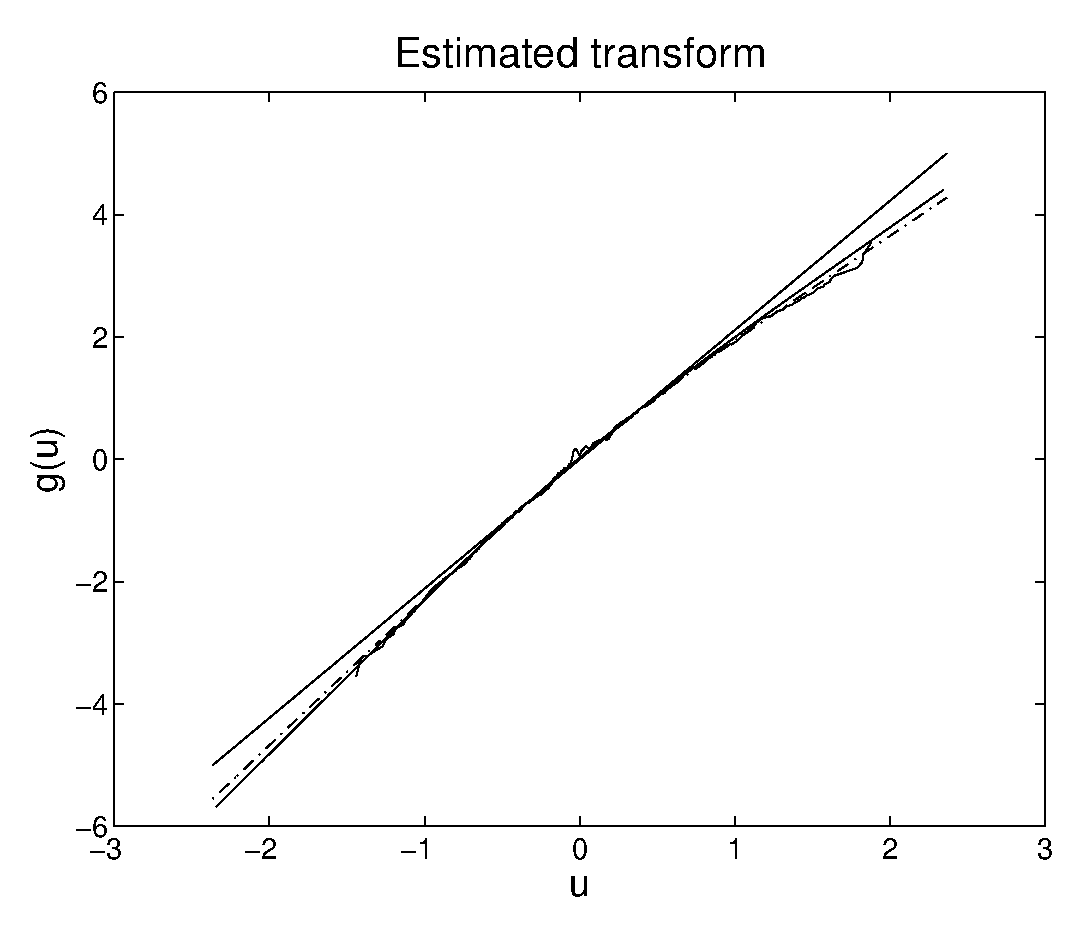
\includegraphics[width=\narrowfigwidth]{fig4grec}
\vspace{-3mm}
\caption[Transformation computed from reconstructed signal]{
The transformation computed from the reconstructed signal
{\tt y} (solid line) compared with
the transformation computed from the original signal {\tt xx}
(dashed dotted line).
}
\label{fig4-11}
\end{figure}

The value of the {\tt test} variable for the transformation
{\tt grec} is 0.84 and, as
expected, it is smaller than the value of {\tt test0} = 1.00 computed for the
transformation {\tt glc}. However, it is still significantly larger then the
values shown in Figure~\ref{fig2-3}, i.e.\ the signal {\tt y} is not
a Gaussian signal.

We turn now to estimation of the spectrum in the model from the simulated
data but first we transform data to obtain a sample $\tilde x(t)$:
{\small\begin{verbatim}
      L = 200
      x = dat2gaus(y,grec); %Gaussian process from reconstructed data
      SSx = dat2spec(x,L);  %Spectrum from Gaussian reconstructed process
\end{verbatim}}
\noindent
The important remark here is that the smoothing of the spectrum defined
by the parameter {\tt L}, see {\tt help dat2spec}, removes almost
all differences between the spectra in the three signals {\tt xx}, {\tt y},
and {\tt x}.
(The spectrum {\tt SSx} is normalized to have first spectral moment one
and has to be scaled down to have the same energy as the spectrum {\tt SS1} on page~\pageref{page:SS1}.)

Next, we shall simulate a random function equivalent to the reconstructed
measurements {\tt y}. The Nyquist frequency gives us the time sampling
of the simulated signal,
{\small\begin{verbatim}
      dt = spec2dt(Sx)
\end{verbatim}}\index[xcmds]{{\tt spec2dt}}
\noindent
and is equal to 0.25~seconds, since the data has been sampled with a
sampling frequency of 4~Hz. We then simulate 2~minutes
($2\times 60\times 4$ points) of the signal, to obtain a
synthetic wave equivalent to the reconstructed non-Gaussian
sea data.
{\small\begin{verbatim}
      Ny = fix(2*60/dt)  % = two minutes
      SSx.tr = grec;
      ysim = spec2sdat(SSx,Ny);
      waveplot(ysim,'-')
\end{verbatim}}
\noindent The result is shown in Figure~\ref{fig_2minutes}.
\end{rtex}

\begin{figure}
\centering
  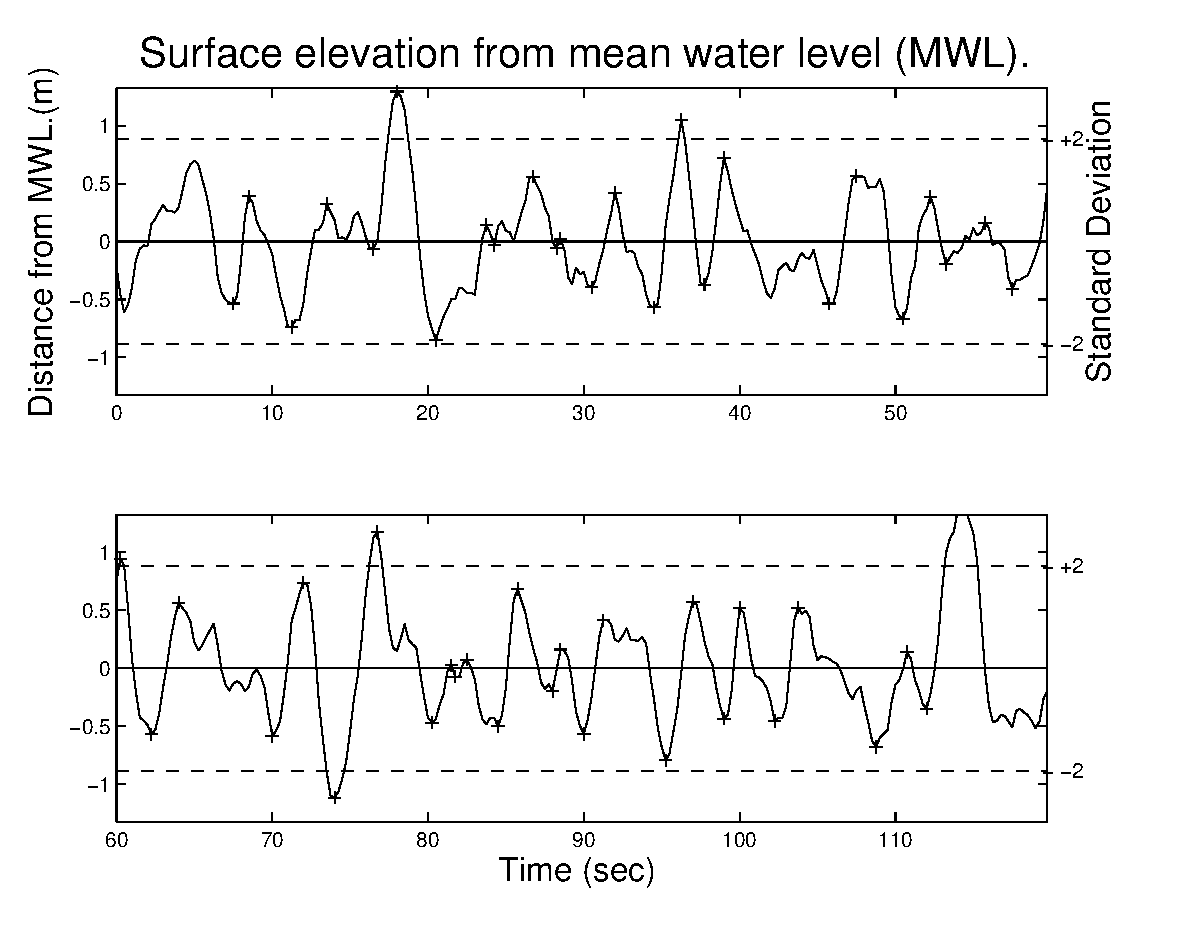
\includegraphics[width=\narrowfigwidth]{fig_2minutes}
\vspace{-3mm}
\caption[Two minutes of simulated sea data]{%
Two minutes of simulated sea data, equivalent to the
  reconstructed data.}
\label{fig_2minutes}
\end{figure}

In the next example we consider a signal with a given theoretical spectrum.
Here we have a problem whether the theoretical spectrum is valid for
the transformed Gaussian model, i.e.\ it is a spectrum $S(\omega)$ or is
it the spectrum of the linear sea $\widetilde S$. In the previous example
the spectrum of the transformed process was almost identical with the
normalized spectrum of the original signal. In
\cite{RychlikEtal1997Modelling} %Rychlik et al (1997)
it was observed that for sea data the spectrum estimated from
the original signal and that for the transformed one do not
differ significantly. Although more experiments should be done in order to
recommend using the same spectrum in the two cases,
here, if we wish to work with non-Gaussian models with
a specified transformation, we shall derive the $\widetilde S$ spectrum
by dividing the theoretical spectrum
by the square root of the first spectral moment of $S$.

\begin{cex}{Ex_sea_simulation}
Since the spectrum {\tt SS1} in Figure~\ref{fig2_spc}
is clearly two-peaked with peak frequency
$T_p = 1.1$ [Hz] we choose to use the Torsethaugen spectrum.
(This spectrum is derived for a specific location and we should not
expect that it will work well for our case.) The inputs to the programs are
$T_p$ and $H_s$, which we now compute.
{\small\begin{verbatim}
      Tp = 1.1;
      H0 = 4*sqrt(spec2mom(S1,1))
      ST = torsethaugen([0:0.01:5],[H0  2*pi/Tp]);
      plotspec(SS1), hold on
      plotspec(ST,[],'-.')
\end{verbatim}}
\noindent
In Figure~\ref{fig4-12}, we can see that the Torsethaugen spectrum
has too little energy on the swell peak. Despite this fact we shall use
this spectrum in the rest of the example.
\begin{figure}
\centering
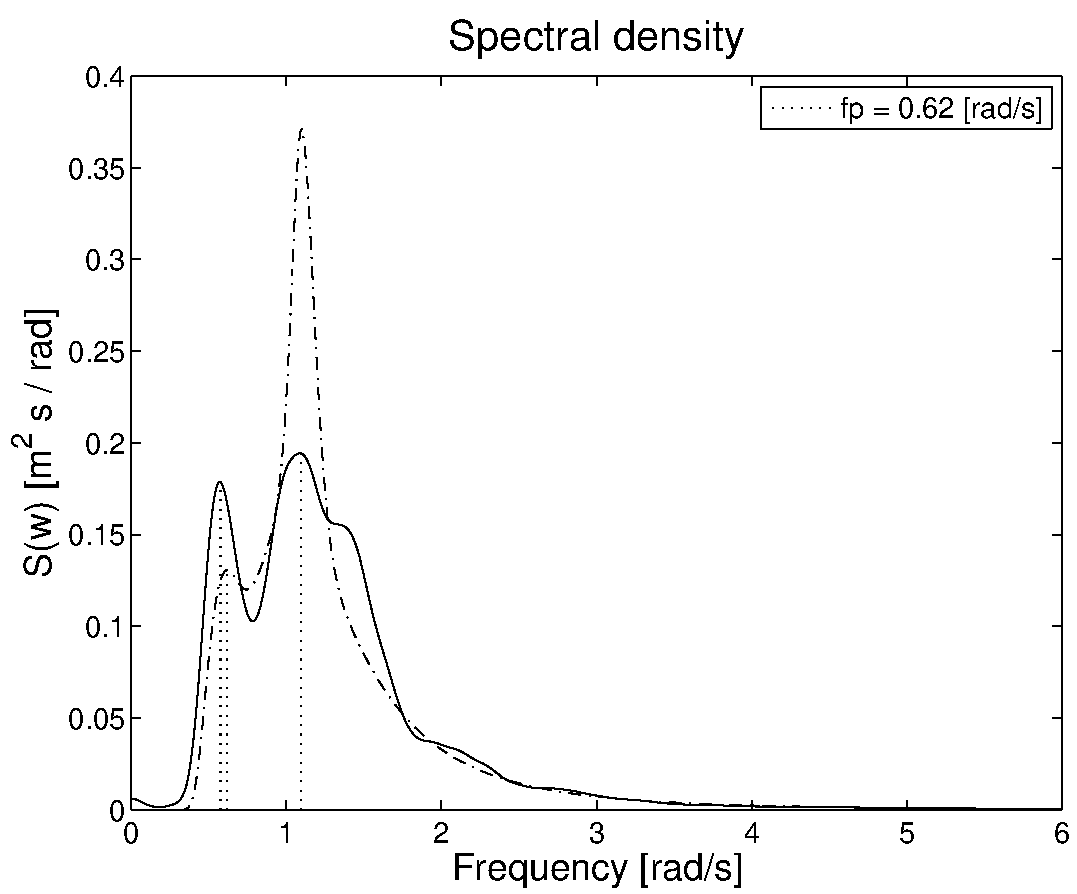
\includegraphics[width=\narrowfigwidth]{fig4spec}
\vspace{-3mm}
\caption[Comparison between spectra of
{\tt sea.dat}]{
Comparison between the estimated spectrum {\tt SS1} in the signal
{\tt sea.dat} (solid line) and the theoretical spectrum {\tt ST} of the
Torsethaugen type (dash-dotted line).
}
\label{fig4-12}
\end{figure}

We shall now create the spectrum $\tilde S(\omega)$ (= {\tt STnorm}),
i.e.\ the
spectrum for the standardized Gaussian process ${\widetilde X}(t)$ with
standard deviation equal to one.
{\small\begin{verbatim}
      STnorm = ST;
      STnorm.S = STnorm.S/sa^2;
      dt = spec2dt(STnorm)
\end{verbatim}}
The sampling interval {\tt dt} = 0.63 [s] (= $\pi / 5$),
is a consequence of our choice of
cut off frequency in the definition of the {\tt ST} spectrum.
This will however not affect our simulation, where any sampling interval
{\tt dt} can be used.

Next, we recompute the theoretical transformation {\tt gh}.
{\small\begin{verbatim}
      [Sk Su] = spec2skew(ST);
      sa = sqrt(spec2mom(ST,1));
      gh = hermitetr([],[sa sk ku me]);
      STnorm.tr = gh;
\end{verbatim}}

\noindent
The transformation is actually almost identical to {\tt gh} for
the spectrum {\tt SS1}, which can be seen in Figure~\ref{fig4_tr},
where it is compared to the Gaussian model {\tt g},
given by a straight line. We can see from the diagram that
the waves in a transformed Gaussian process $X(t)=G({\widetilde X}(t))$,
will have an excess of high crests and shallow troughs compared to
waves in the Gaussian process $\widetilde X(t)$. The difference is
largest for extreme waves with crests above 1.5~meters, where
the excess is 10~cm, ca~7~\%.
Such waves, which have crests above three standard deviations,
are quite rare and for moderate waves the difference is negligible.

In order to illustrate the difference in distribution for extreme waves
we will simulate a sample of 4~minutes of $X(t)$ with sampling
frequency 2~Hz. The result is put into \verb+ysim_t+.
In order to obtain the corresponding sample
path of the process $\widetilde X$ we use the transformation {\tt gh},
stored in {\tt STnorm.tr}, and put the result in \verb+xsim_t+.
{\small\begin{verbatim}
      dt = 0.5;
      ysim_t = spec2sdat(STnorm,240,dt);
      xsim_t = dat2gaus(ysim_t,STnorm.tr);
\end{verbatim}}
Since the process $\tilde X(t)$ always has variance one, in order to
compare the Gaussian and non-Gaussian models we scale
\verb+xsim_t+ %{\tt xsim$_t$}
to have the same second spectral moment as
\verb+ysim_t+,  %{\tt ysim$_t$},
which will be done by the following commands:
{\small\begin{verbatim}
      xsim_t(:,2) = sa*xsim_t(:,2);
      waveplot(xsim_t,ysim_t,5,1,sa,4.5,'r.','b')
\end{verbatim}}
\begin{figure}[t]
\centering
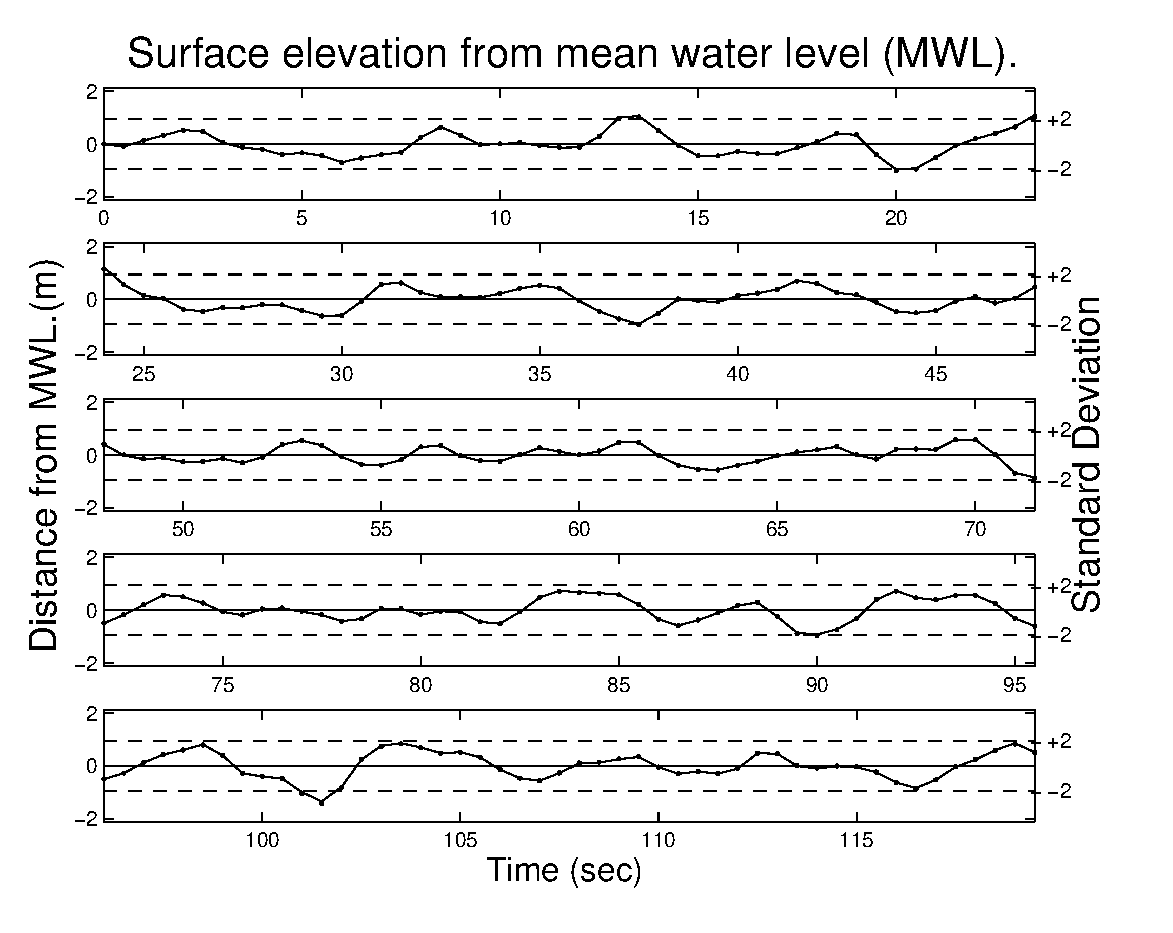
\includegraphics[width=\narrowfigwidth]{figure_sim1}
\vspace{-3mm}
  \caption[Gaussian simulated and transformed signals]{%
Simulated  $X(t)=G(\widetilde X(t))$ (solid line) compared
    with $\widetilde X(t)$ (dots) scaled to have the same $H_s$ as $X(t)$ for
    a theoretical
    spectrum  given by Torsethaugen spectrum {\tt St}.}
  \label{fig4-2}
\end{figure}

In Figure~\ref{fig4-2} we have waves that are not
extremely high and hence the difference between the two models is
hardly noticeable in this scale. Only in the second subplot we can see
that Gaussian waves (dots) have troughs deeper and crests lower than
the transformed Gaussian model (solid line). This also indicates
that the amplitude estimated from the transformed Gaussian and Gaussian
models are practically identical. Using the empirical transformation
{\tt glc} instead of the Hermite transformation
{\tt gh} would give errors of ca 11\%,
which for waves with higher significant wave height would give considerable
underestimation of the crest height of more extreme waves.
Even if the probability for observing an extreme wave during
the period of 20 minutes is small, it is not negligible for safety
analysis and therefore the choice of transformation is one of the most
important questions in wave modelling.

Since the difference between Gaussian and non-Gaussian model is not
so big we may ask whether 20 minutes of observation
of a transformed Gaussian process presented in this example is long enough
to reject the Gaussian model. Using the function {\tt testgaussian}
we can see that rejection of Gaussian model would occur very seldom.
Observe that the {\tt sea.dat} is 40 minutes long and that we
clearly rejected the Gaussian model.
\end{cex}


\index[xentr]{transformed Gaussian models|)}
\index[xentr]{transformed Gaussian models!simulation of|)}
\index[xentr]{simulation!of transformed Gaussian process|)}

\section{More on simulation  with \wf{}}\label{s:2.4}
The \wf{} toolbox contains additional routines for simulation of 
random loads and random waves. 
One important class used in fatigue analysis and in modelling
the long term variability of sea state are the Markov models, 
in which the model parameters are allowed to switch to new 
values according to a Markov chain.\index[xentr]{Markov!chain}
Another group of simulation routines generate non-linear waves and loads, 
like second order Stokes waves with interaction between 
frequency components in the Gaussian wave model, and 
Lagrange waves, with a horizontal deformation of  space. 
This  group includes a program to simulate the output of second
order oscillators with nonlinear spring,  when external force is
white noise. The nonlinear oscillators can be used to
model nonlinear responses of sea structures.

\subsection{Markov models}
The following routines from the {\tt simtools} module can be used to generate realistic 
load sequencies  for for reliability and fatigue analysis; see more in Chapter~\ref{cha:5}.
\begin{description}
\item[{\tt lc2sdat}] Simulates a load process with specified crossing spectrum and irregularity
\item[{\tt mcsim}] Simulates a finite Markov chain from its probability transition matrix
\item[{\tt mctpsim}] Simulates a Markov chain of turning points from transition matrix
\item[{\tt sarmasim}] Simulates an ARMA time series with Markov switching parameters
\item[{\tt smcsim}] Simulates a Markov chain with Markov switching regime
\end{description}

\begin{rtex}{SARMA}{Switching ARMA model}
In many applications, the standard stationary  time series Auto-regressive/Moving average ARMA-model, 
\cite[Ch.~7]{LindgrenRootzenSandsten2014}, can be made more realistic if the 
parameters are allowed to change with time, according to abrupt changes in environment conditions. 
Examples are found in econometrics \cite{Hamilton1989}, climate and environmental research \cite{AilliotMonbet2012}, automotive safety   \cite{Johannesson1998Rainflow}, and many other areas. 
A special case are the {\it Hidden Markov models} where the changes occur according to an 
(unobserved)  Markov chain

The \wf{} routine {\tt sarmasim} was developed by  Johannesson \cite{Johannesson1998Rainflow} 
in order to find a good model for stress loads on a truck serving on an irregular scheme, loading 
and unloading gravel. 
 The following example from {\tt sarmasim} illutrates the principles on an ARMA(4,2)-process swhitching
by a Markov {\it regime process} between two states.  \index[xentr]{Markov!hidden model}
\index[xcmds]{{\tt sarmasim}}
{\small\begin{verbatim}
    p1 = 0.005; p2=0.003;  % Switching probabilities
    P = [1-p1 p1; p2 1-p2];  % Markov transition matrix
    C = [1.00 1.63 0.65; 1.00 0.05 -0.88];  % MA-parameters 
    A = [1.00 -0.55 0.07 -0.26 -0.02; ... 
    		   1.00 -2.06 1.64 -0.98 0.41];  % AR-parameters
    m = [46.6; 7.4]*1e-3;  % Mean values for sub-processes
    s2 = [0.5; 2.2]*1e-3;  % Innovation variances
    [x,z] = sarmasim(C,A,m,s2,P,2000);  % Simulate 2000 steps
    plothmm(x,z)  % Ploting
    		   %  x = Switching ARMA, z = Markov regime process
\end{verbatim}}
Figure~\ref{fig:sarmasim} shows the hidden Markov states and the, seemingly non-stationary,  
ARMA-process. In fact, the Markov chain is simulated from its stationary distribution and each 
ARMA-section starts with the stationary distribution for that particular ARMA-process, so 
the process is stationary! 
\end{rtex}
\begin{figure}[tbh]
\centerline{
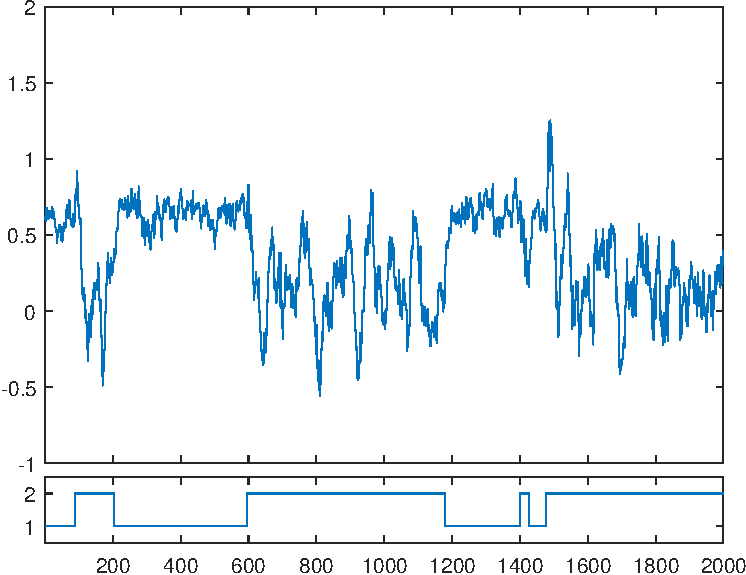
\includegraphics[width=\narrowfigwidth]{sarmasim}
}
\caption{Switching ARMA-process with Markov regime process.}
\label{fig:sarmasim}
\end{figure}


\subsection{Space-time and non-linear waves and loads}
The following routines in modules {\tt simtools} and {\tt lagrange} generate 
continuous time series and continuous space-time realizations. 
\begin{description}
\item[{\tt duffsim}] Generates a sample path of a 
linear or non-linear random oscillator \index[xcmds]{{\tt duffsim}}
\item[{\tt spec2wave} and {\tt spec2field}] Generate samples of space-time 
(transformed) \index[xcmds]{{\tt spec2field}}
 2D and 3D Gaussian waves  \index[xcmds]{{\tt spec2wave}}
\item[{\tt seamovie}] Makes a movie in time of 2D or 3D random waves
and optionally exports movie in {\tt avi} format  \index[xcmds]{{\tt seamovie}}
\item[{\tt seasim}] Old routine that generates a space-time Gaussian process and movie 
with 1D or 2D space parameter \index[xcmds]{{\tt seasim}}
\item[{\tt spec2ldat} and {\tt spec2ldat3D}] Routines in module {\tt lagrange} that generate 
front-back and crest-trough asymmetric \index[xcmds]{{\tt spec2ldat}}
modifications of Gaussian wave fields
\item[{\tt spec2nlsdat}] Simulates a random 2nd order \index[xcmds]{{\tt spec2nlsdat}}
non-linear wave from a spectral density
\end{description}

\begin{rtex}{Seamovieforexport}{How to export a sea movie}
In Section~\ref{ss:dirspec} we gave an example of how to use {\tt spec2field} 
to generate and plot a Gaussian sea surface with directional spreading. We now show how to 
use {\tt seamovie} to generate and save a movie of the time evolution of the sea. 

We define and plot the {\tt demospec} spectrum, with frequency independent 
spreading \index[xcmds]{{\tt demospec}}
{\small\begin{verbatim}
    SD = demospec('dir')
    plotspec(SD)
\end{verbatim}}
\noindent to get Figure~\ref{fig:demospec} and the structure
{\small\begin{verbatim}
SD = 
  struct with fields:
          S: [101 x 257 double]
        w: [257 x 1 double]
    theta: [101 x 1 double]
       tr: []
        h: Inf
     type: 'dir'
      phi: 0
     norm: 0
     note: 'Demospec: JONSWAP, Hm0 = 7, Tp = 11, gamma = 2.3853; Sprea...'
\end{verbatim}
}

\sidecaptionvpos{figure}{c}
%\begin{SCfigure}[0.75][t]
\begin{figure}[t]
\centerline{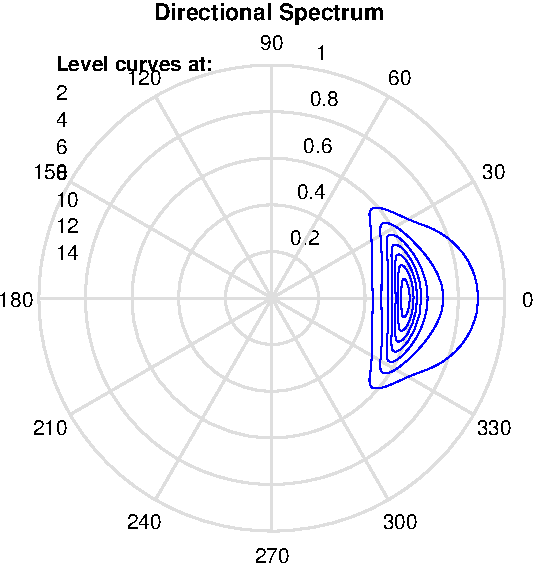
\includegraphics[width=0.5\textwidth]{fig_demospec}}
\caption[Directional spectrum {\tt demospec}]{Directional spectrum {\tt demospec}}
\label{fig:demospec}
%\end{SCfigure}
\end{figure}

To generate two minutes of a wave field of size 500[m] by 250[m] we define parameters 
by the function 
{\tt simoptset}\index[xcmds]{{\tt simoptset}}, 
generate the field with 
{\tt spec2field}\index[xcmds]{{\tt spec2field}}, 
and make three different types of movies with {\tt seamovie}\index[xcmds]{{\tt seamovie}}.  
{\small\begin{verbatim}
    opt = simoptset('Nt',600,'dt',0.2,'Nu',501','du',1,'Nv',251,'dv',1)
    rng('default')
    W = spec2field(SD,opt);  % structure with fields .Z, .x, .y, .t
    figure(2); Mv2 = seamovie(W,2); pause
    figure(3); Mv3 = seamovie(W,3); pause
    figure(1); Mv1 = seamovie(W,1,'sea.avi')
 \end{verbatim}}
\noindent The last movie command saves the movie as {\tt sea.avi} in the working directory. 
If {\tt sea.avi} already exists, the new movie file is given a random name. 
\end{rtex}

\begin{figure}
\centerline{
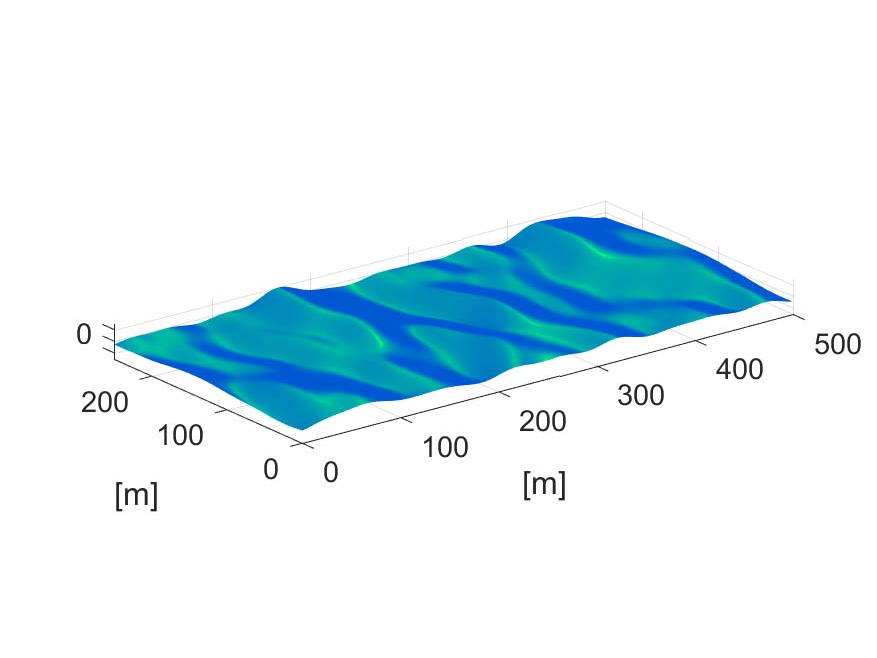
\includegraphics[width=130mm]{Mv1}
}
\vspace{3mm}
\centerline{
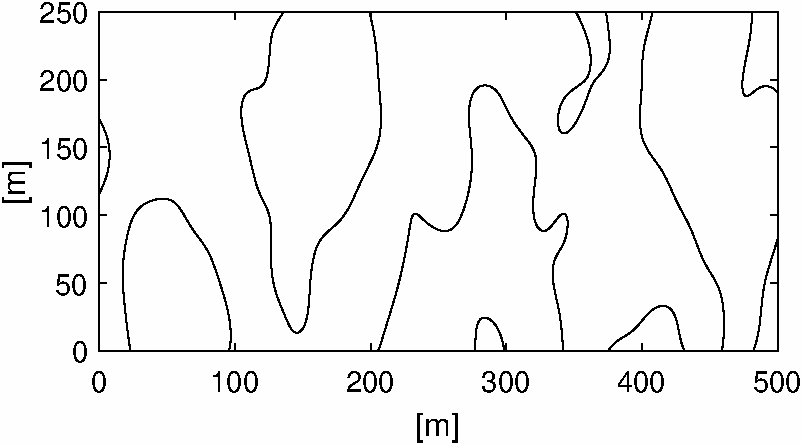
\includegraphics[width=130mm]{Mv2}
}\vspace{3mm}
\centerline{
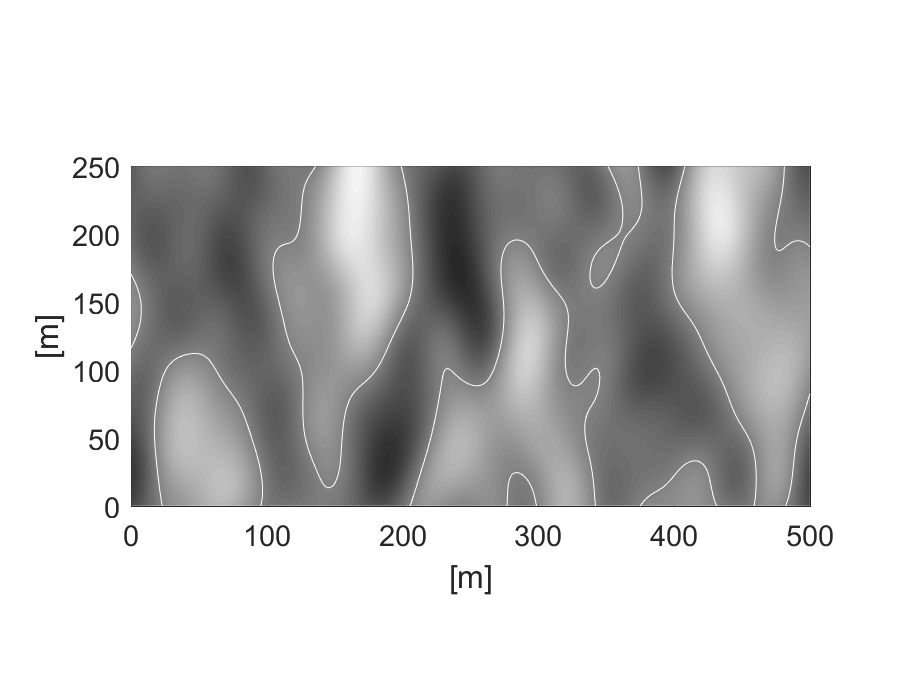
\includegraphics[width=130mm]{Mv3}
}
\vspace{-1mm}
\caption[Three aspects of Gaussian wave field]%
{Three aspects of a simulated Gaussian wave field with directional spectrum {\tt demospec('dir')}; last frames in 
{\tt Mv1}, {\tt Mv1}, and {\tt Mv3}.}
\label{Fig:threefields}
\end{figure}

\begin{remark}
The wave fields generated by {\tt spec2field} differ from animated wave fields used for example 
in feature films. They are intended to be used in applications where the fine structure, 
so important for the visual impression,  can be neglected. Examples involve extreme value analysis, 
fatigue loads, and ship dynamics.
\end{remark}

%\clearpage
\subsection{Structure of spectral simulation}
The following table explaines the sequencing of spectral simulation routines in modules {\tt simtools} and {\tt lagrange}. 
A (freq) or (dir) indicates the type of input spectrum.   
\vspace{5mm}

\begin{turn}{90}
\centering
\setlength\extrarowheight{3pt}
\begin{tabular}{||l|c|c|c|c||}\hline\hline 
\multicolumn{5}{||c||}{} \\
 \multicolumn{5}{||c||}{\raisebox{10pt}{\large \fo and \so order Gaussian waves in module {\tt simtools}}} \\ \hline
Routine & {\tt spec2sdat} & {\tt spec2wave} & {\tt spec2field} & {\tt spec2nlsdat}\\ \hline 
Type & \fo order Gaussian  & \fo order Gaussian  & \fo order Gaussian  & \so order Gauss-Euler \\
& time or space series & 2D space-time wave & 3D space-time field & 2D time wave \\
 & $\downarrow$ & $\downarrow$ & $\downarrow$ & $\downarrow$\\
Output & {\tt [x,xder]} & {\tt W.Z, .x, .t}& {\tt W.Z, .x, .y, .t} & {\tt [xs2,xs1]}\\
& & $\downarrow$ & $\downarrow$ & \\
Movie & & {\tt M = seamovie(W,type)} & {\tt M = seamovie(W,type)} &\\ \hline\hline 
\multicolumn{5}{||c||}{}  \\
 \multicolumn{5}{||c||}{\raisebox{10pt}{\large \fo and \so order Lagrange waves in module {\tt lagrange}}} \\ \hline
Routine & {\tt spec2ldat } (freq) & {\tt spec2lseries } (dir)  & {\tt spec2ldat3D } (dir)& {\tt spec2ldat3DM/P}\\ \hline 
Type & \fo order Lagrange 2D & \fo order Lagrange 2D & \fo order Lagrange 3D & \so order Lagrange 3D \\
& space/time components & time series & space/time components & space/time components\\
& $\downarrow$ & $\downarrow$ & $\downarrow$ & $\downarrow$\\
Output & {\tt [w,x]} & {\tt L.Z, .t, .points}& {\tt [w,x,y]}& {\tt [w,x,y,w2,x2,y2]}\\
& $\downarrow$ & $\downarrow$ & $\downarrow$ & $\downarrow$\\
Series/field & {\tt L = ldat2lwav} & \rule{7mm}{0.5mm}  & {\tt L = ldat2lwav3D} & {\tt L = ldat2lwav3D} \\
& $\downarrow$ & $\downarrow$ & $\downarrow$ & $\downarrow$\\
Movie &{\tt M = seamovie(L,type)} & {\tt M = seamovie(L,type)} & {\tt M = seamovie(L,type)} &{\tt M = seamovie(L,type)}\\ \hline\hline 
\end{tabular} 
\end{turn}

%\svnInfo $Id: Ch3_2017.tex 65 2017-08-14 19:39:16Z Georg Lindgren $ 
%$
%
\chapter[Empirical wave characteristics]{%
Empirical wave characteristics}
\label{cha:distr-appar-wave-data}\label{cha:3}

%=====================
%---------------------
%=====================
One of the unique capabilities of \progname{} is the treatment of
the statistical properties of wave characteristic. This, and the next chapter,
describe how to extract information on distributions of observables like
wave period, wave length, crest height, etc, either directly from data, or
from empirically fitted approximative models, or, in the next chapter, by means
of exact statistical distributions, numerically computed from a spectral model.

We first define the different wave characteristics commonly used in
oceanographic engineering and science, and present the \progname{} routines
for handling them. Then we compare the empirical findings with some
approximative representations of the statistical distributions, based
on empirical parameters from observed sea states. The code for the examples
are found in the m-file \verb+Chapter3.m+, and it takes a few seconds to run.

\section{Introduction}
\index[xentr]{wave characteristics|(}
\subsection{The Gaussian paradigm - linear wave theory}\label{ss:gaussianparadigm}
\index{linear wave theory}
In the previous chapter we discussed modelling of random functions by
means of Fourier methods. The signal was represented as a sum of
independent random cosine functions with random amplitudes and phases. In linear
wave theory those cosine functions are waves travelling in water. Waves
with different frequencies have different speeds, defined by the
dispersion relation. \index[xentr]{dispersion relation}
This property causes the characteristic
irregularity of the sea surface. Even if it were possible to arrange a very
particular combination of phases and amplitudes, so that the signal
looks, for example, like a saw blade, it will, after a while, change
shape totally. The phases will be almost independent and the sea would
again look like a Gaussian random process. On the other hand an
observer clearly can identify moving  sea waves. The shape of those
waves, which are often called the
{\sl apparent  waves},\index[xentr]{apparent!wave}
since theoretically, those are not mathematical waves, but are constantly
changing up to the moment when they disappear.

The wave action on marine structures is often modelled using linear filters.
Then the sea spectrum, together with the filter frequency function,
gives a complete characterization of the response
of the structure. However, often such models are too simplistic
and non-linearities have to be considered to allow more complex responses.
Then one may not wish to perform a complicated numerical
analysis to derive the complete response but is willing to accept
the simplification that the response is proportional to the waves.
One may also wish to identify some properties of waves that are dangerous
in some way for the particular ocean operation.
Also the apparent waves themselves can be the reason for non-linear response.
For example, for waves with crests higher than some
threshold, water may fill a structure and change its dynamical properties.
The combined effect of apparent waves, often described by their
height and wave period, is therefore important in ocean engineering.
These aspects are discussed in more detail in
the textbook \cite{Ochi1998Ocean}.

The apparent waves will be described by some geometric properties,
called wave characteristics, while frequencies of
occurrences of waves with specified characteristics will be treated in the
statistical sense and described by a probability distribution. Such
distributions can then be used to estimate the frequency of occurrences
of some events important in the design of floating marine systems,
e.g.\ wave breaking, slamming, ringing, etc.

\subsection{Wave characteristics in time and space}
The wave surface is clearly a two-dimensional phenomenon that changes
with time and its study naturally deals with moving two-dimensional
objects (surfaces). Theoretical studies of random surfaces are the 
subject of ongoing research, for example,
\cite{AzaisWschebor2009,Mercardier2006},
for general studies of Gaussian random surfaces, 
\cite{Aberg2007diss,AbergRychlikLeadbetter2008,BaxevaniEtal2003Velocities,
BaxevaniRychlik2006,PodgorskiEtal2000Statistics,Sjo2000Crossing,Sjo2001Simultaneous}, 
for space-time related wave results, and \cite{PodgorskiRychlik2016SizeOfWaves} 
for wave geometry. 
Related results for Lagrange models are found in
\cite{AbergLindgren2008,Lindgren2006,Lindgren2009,Lindgren2010a,
LindgrenAberg2009,Lindgrenetal2010}.

At present, there are only few programs in \progname{} that
handle the space-time relations of waves, and hence in this tutorial we limit 
the presentation to simpler cases of waves in one-dimensional \index[xentr]{Lagrange waves}
records.\footnote{The Lagrange module in \progname{} contains special  
space-time routines for (Gaussian and) non-Gaussian waves; a tutorial is included in that module.} 
By this we mean the apparent waves extracted from functions
(measured signals) with one-dimensional parameter, either in time or in
space. These functions can be extracted from a photograph of the sea
surface as, for example, the {\it instantaneous profile} along a line
in some fixed horizontal direction on the sea, or they can be obtained
directly as a {\em record taken in time at a fixed position in space}
as by means of a wave pole or distance meter.  The
{\em encountered sea},\index[xentr]{encountered sea}
another important one-dimensional record, can be collected
by means of a ship-borne wave recorder moving across the random sea.

To analyze collected wave data we need natural and operational
definitions of an individual wave, its period, height, steepness, and
possibly some other meaningful characteristics. There are several
possible definitions of apparent wave, and here we shall concentrate
mostly on zero down-crossing waves. Namely, the
{\em apparent individual wave}
at a fixed time or position is defined as the part
of the record that falls between two consecutive down-crossings of the
zero seaway level (the latter often more descriptively referred to as
the still water level).  For individual waves one can consider various
natural characteristics, among them {\em apparent periods}  and
{\em apparent heights (amplitudes)}. The pictorial definitions of these
characteristics are given in \index[xentr]{apparent!period}
Figure~\ref{fig:wavpar}. \index[xentr]{apparent!height}
\begin{figure}[tbh]
\centering
  %\includegraphics[width=0.6\textwidth,angle=-90]{005f_wvp}
  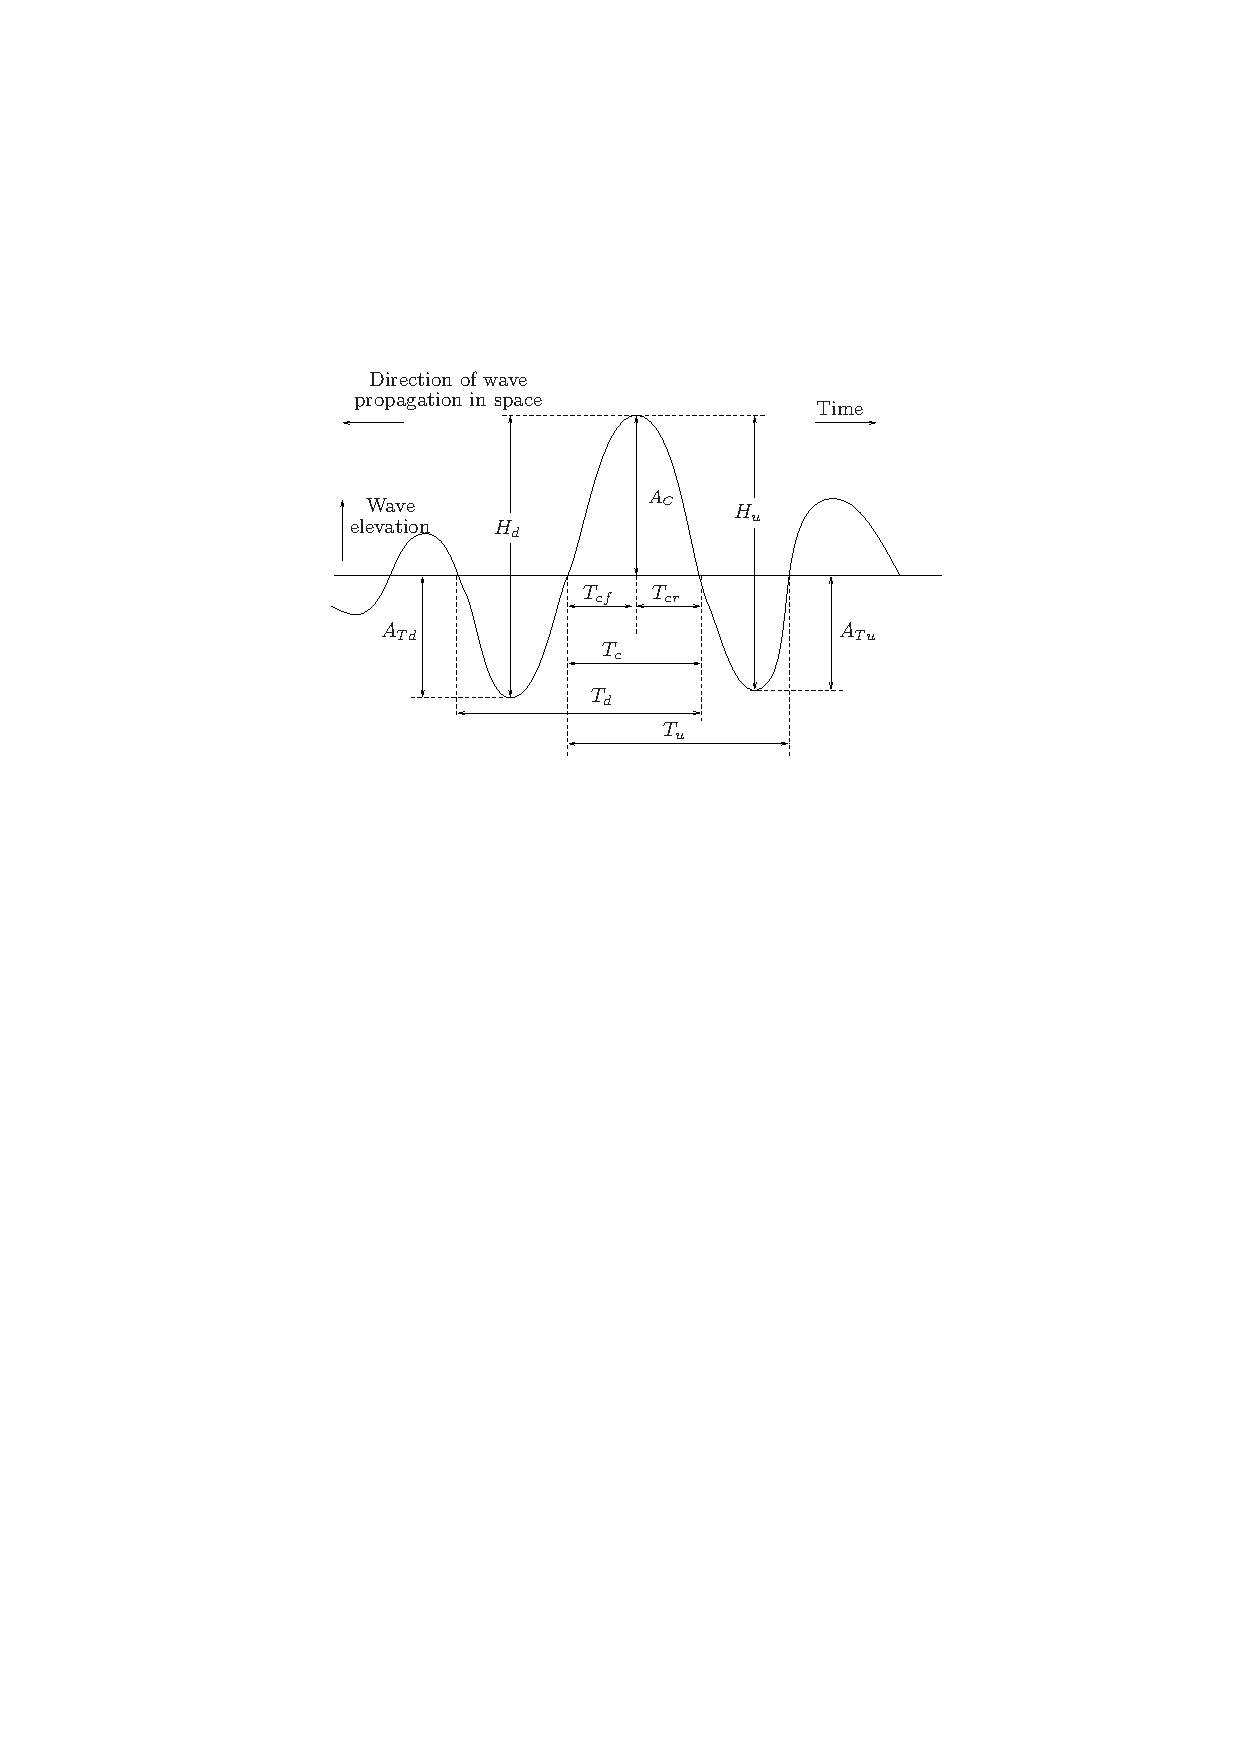
\includegraphics[width=0.7\textwidth,angle=0]{waveparamNew}
\vspace{-3mm}
  \caption[Definition of wave parameters]
{Definition of wave parameters. The notation for the parameters
used in our examples are given in Table~\ref{tab3_1} at the end of this chapter.}
  \label{fig:wavpar}
  \end{figure}

The definitions of the most common wave characteristics are given in
Table~\ref{tab3_1}. In the \progname{} toolbox, the most important can be
retrieved by the help commands for {\tt wavedef}, {\tt perioddef},
{\tt ampdef}, and {\tt crossdef}, producing the output in
Section~\ref{sec:WAFOcharacteristics}.
\index[xcmds]{{\tt wavedef}}
\index[xcmds]{{\tt perioddef}}
\index[xcmds]{{\tt ampdef}}
\index[xcmds]{{\tt crossdef}}

Having precisely defined the characteristics of interest, one can
extract their frequency (empirical) distributions from a typical
sufficiently long record.  For example, measurements of the apparent
period and height of waves could be taken over a long
observation interval to form an empirical two-dimensional
distribution. This distribution will represent some aspects of a given
sea surface. Clearly, because of the irregularity of the sea,
empirical frequencies will vary from record to record. However if the
sea is in ``steady'' condition, which corresponds mathematically to
the assumption that the observed random field is stationary and
ergodic, their variability will be insignificant for sufficiently
large records. Such limiting distributions (limiting with respect to
observation time, for records measured in time, increasing without
bound) are termed the
{\em long-run distributions}. \index[xentr]{long-run distribution}
Obviously, in a real 
sea we seldom have a so long period of "steady" conditions that the
limiting distribution will be reached. On average, one may observe
400-500 waves per hour of measurements, while the stationary
conditions may last from 20 minutes to only a few hours.

Despite of this, a fact that makes these long-run distributions particularly
attractive is that they give probabilities of occurrence of waves that
may not be observed in the short records but still are possible. Hence,
one can estimate the intensity of occurrence of waves with special
properties and then extrapolate beyond the observed types of waves.
What we shall be concerned with next is how to compute such
distributional properties.

In the following we shall consider three different ways to
obtain the wave characteristic probability densities (or
distributions):

\begin{itemize}
\item
To fit an empirical distribution to observed (or simulated) data in
some parametric family of densities, and then relate the estimated
parameters to some observed wave climate described by means of
significant wave heigh and wave period. Algorithms to extract
waves, estimate the densities and compute some simple statistics will
be presented here in Chapter~\ref{cha:3}

\item
To simplify the model for the sea surface to such a degree that
explicit computation of wave characteristic densities (in the
simplified model) is possible. Some examples of proposed models from
the literature will also be given in this chapter.

\item
To exactly compute the statistical distribution from the mathematical form of a
random seaway. This requires computation of infinite
dimensional integrals and expectations that have to be
computed numerically. \progname{} contains efficient numerical
algorithms to compute these integrals, algorithms which do not require
any particular form of the sea surface spectrum.
The method are illustrated in Chapter~\ref{cha:4}
on period, wavelength, and amplitude
distributions, for many standard types of wave
spectra.
\end{itemize}

\section{Estimation of wave characteristics from data}
\label{sec:estim-wave-char}
\index[xentr]{wave characteristics!estimation from data|(}

In this section we shall extract the wave characteristics from a
measured signal and then use non-parametric statistical methods
to describe the data, i.e.\ empirical distributions, histograms,
and kernel estimators.
(In the last chapter of this tutorial  we present some statistical
tools to fit parametric models; for kernel estimators, see Appendix~\ref{cha:KDE}.)

It is generally to be advised that, before analyzing sea wave
characteristics, one should check the quality of the data by inspection
and by the routine \verb+findoutliers+ used in Section~\ref{sect2.1}.
Then, one usually should remove any present trend
from the data. Trends could be due to tides or atmospheric pressure
variations that affect the mean level. De-trending can be done using the
\progname{} functions {\tt detrend}\index[xcmds]{{\tt detrend}} or
{\tt detrendma}\index[xcmds]{{\tt detrendma}}.
\index[xcmds]{{\tt findoutliers}}

\subsection{Wave period}
\index[xentr]{wave distributions!estimation of densities!wave period}
\begin{cex}{Ex_sea_statistics}
We now continue the analysis of the shallow water waves in {\tt sea.dat} that 
we started on page~\pageref{pageseadat}. 
We begin with extracting the apparent waves
\index[xentr]{apparent wave!extraction of} and record their period.
The signal  {\tt sea.dat} is recorded at 4~Hz sampling frequency.
One of the possible definitions of period is the time between the
consecutive wave crests. For this particular variable it may be
convenient to have a higher resolution than 4~Hz and hence we shall
interpolate the signal to a denser grid. This will be obtained by giving
an appropriate value to the variable {\tt rate} which can be used as input
to the \progname{} routine \verb+dat2wa+\index[xcmds]{{\tt dat2wa}}.
The following \index[xcmds]{{\tt rate}}
code will return crest2crest wave periods $T_{cc}$ in the variable
{\tt Tcrcr} and return the crest period $T_c$ in {\tt Tc}, i.e.\ the time from
up-crossings to the following down-crossing.
{\small\begin{verbatim}
      xx = load('sea.dat');
      xx(:,2) = detrend(xx(:,2));
      rate = 8;
      Tcrcr = dat2wa(xx,0,'c2c','tw',rate);
      Tc = dat2wa(xx,0,'u2d','tw',rate);
\end{verbatim}}

Next we shall use a kernel density estimator
(KDE) \index[xcmds]{{\tt kde}}
to estimate the probability density function (pdf)
of the crest period and compare the resulting pdf with a
histogram of the observed periods stored in {\tt Tc}.
In order to define a suitable scale for the density we first compute the
mean and maximum of the observed \index[xcmds]{{\tt kdeoptse}}
crest periods.
{\small\begin{verbatim}
      mean(Tc)
      max(Tc)
      t = linspace(0.01,8,200);
      kopt = kdeoptset('L2',0);
      ftc1 = kde(Tc,kopt,t);
      pdfplot(ftc1), hold on
      histgrm(Tc,[],[],1)
      axis([0 8 0 0.5])
\end{verbatim}}\index[xcmds]{{\tt kde}}
\noindent
(The parameter {\tt L2=0}  is used internally in  {\tt kde}, and
causes a logarithmic transformation of the data to ensure that the density
is zero for negative values. Run \verb+help kdeoptset+ to see the definition.)

\begin{figure}
\centering
  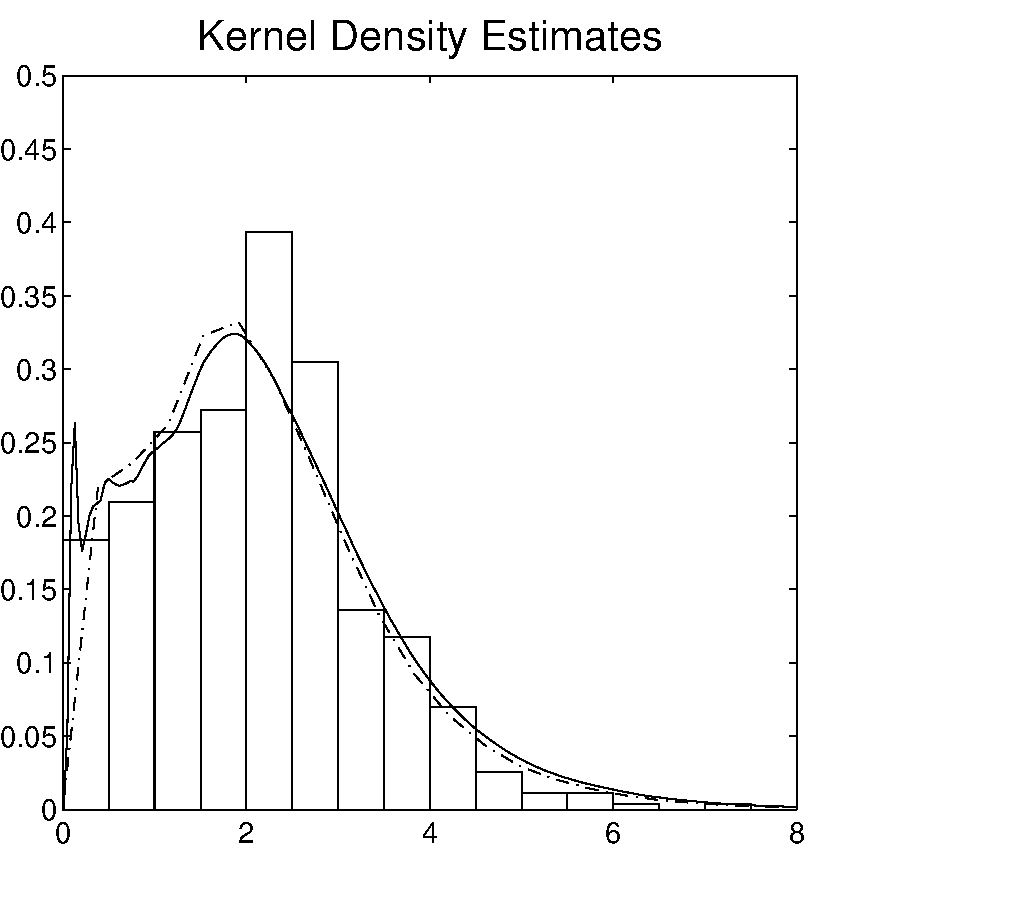
\includegraphics[width=\narrowfigwidth]{fig7_kde_tc}
\vspace{-3mm}
  \caption[Kernel estimate of the crest period density]{
Kernel estimate of crest period density observed in {\tt sea.dat};
solid line: full KDE, dash dotted line: binned KDE,
compared with histogram of the data.
}
  \label{fig7_kde_tc}
\end{figure}
In Figure~\ref{fig7_kde_tc} we can see that many short
waves have been recorded (due to relatively high sampling frequency).
The kernel estimate will be compared with the theoretically
computed density in Figure~\ref{fig73} in Chapter~\ref{cha:4},
%page~\pageref{page:Ex7a}.
page~\pageref{fig73}.
\end{cex}

\begin{remark} Note that the program {\tt kde}
can be quite slow for large data sets. If a faster estimate of the
density for the observations is preferred one can use
{\tt kdebin}\index[xcmds]{{\tt kdebin}},
which is an approximation to the true kernel density estimator. An
important input parameter in the program, that defines the degree of
approximation, is {\tt inc} which should be given a value between 100 and
500. (A value of {\tt inc} below 50 gives fast execution times
but can lead to inaccurate results.)
{\small\begin{verbatim}
      kopt.inc = 128;
      ftc2 = kdebin(Tc,kopt); pdfplot(ftc2,'-.')
      title('Kernel Density Estimates'), hold off
\end{verbatim}}
\noindent The result is in
Figure~\ref{fig7_kde_tc}  \index[xcmds]{{\tt inc}}
\end{remark}

\subsection{Extreme waves -- model check}
We turn now to joint wave characteristics, e.g.\ the joint density of
half period and crest height {\tt (Tc,Ac)}, or waveheight and steepness
{\tt (Ac,S)}. The program {\tt dat2steep} identifies apparent waves and 
for each wave gives several wave characteristics
(use the help function on {\tt dat2steep} for
a list of computed variables). \index[xcmds]{{\tt dat2steep}}
We begin by examining profiles of waves having some special property,
e.g.\ with high crests, or that are extremely steep.

\begin{cex}{Ex_sea_statistics}
The following code  finds a sequence of waves in {\tt sea.dat} and extracts 
their characteristics:
{\small\begin{verbatim}
      method = 0; rate = 8;
      [S, H, Ac, At, Tcf, Tcb, z_ind, yn] = ...
             dat2steep(xx,rate,method);
\end{verbatim}}

The first preliminary analysis of the data is to find the individual waves
which are extreme by some specified criterion, e.g.\ the steepest or the
highest waves, etc. To do such an analysis one can use the function
{\tt spwaveplot(xx,ind)}\index[xcmds]{{\tt spwaveplot}}, which plots
waves in {\tt xx} that are selected by the index variable {\tt ind}.
For example, let us look at the highest and the steepest waves.
{\small\begin{verbatim}
      [Smax indS] = max(S)
      [Amax indA] = max(Ac)
      spwaveplot(yn,[indA indS],'k.')
\end{verbatim}}

The two waves are shown in Figure~\ref{fig_c_wave}(a). The  shape of
the biggest wave reminds of the so called "extreme" waves.
In the following we shall examine whether this particular shape contradicts
the assumption of a transformed Gaussian model for the sea.

This is done as follows. First we find the wave with the highest crest.
Then we mark all positive values in that wave as missing.
Next we reconstruct the signal, assuming the Gaussian model is valid,
and compare the profile of the reconstructed wave with the actual
measurements.
Confidence bands for the reconstruction will also be plotted.
In the previous chapter we have already used the program
{\tt reconstruct}, \index[xcmds]{{\tt reconstruct}} and here
we shall need some additional output from that function, to be used to
compute and plot the confidence bands.
{\small\begin{verbatim}
      inds1 = (5965:5974)'; Nsim = 10;
      [y1, grec1, g2, test, tobs, mu1o, mu1oStd] = ...
             reconstruct(xx,inds1,Nsim);
      spwaveplot(y1,indA-10), hold on
      plot(xx(inds1,1),xx(inds1,2),'+')
      lamb = 2.;
      muLstd = tranproc(mu1o-lamb*mu1oStd,fliplr(grec1));
      muUstd = tranproc(mu1o+lamb*mu1oStd,fliplr(grec1));
      plot (y1(inds1,1), [muLstd muUstd],'b-')
      axis([1482 1498 -1 3]), hold off
\end{verbatim}}\index[xcmds]{{\tt tranproc}}

\noindent(Note that we have used the function {\tt tranproc} instead of
{\tt gaus2dat}, since the last function requires a two column matrix.
Furthermore we have to use the index {\tt indA-10} to identify
the highest wave in {\tt y1}. This is caused by the fact that the
interpolated signal {\tt yn} has a few additional small waves that
are not in {\tt xx}.)

\begin{figure}
\subfigure[]{%
\begin{minipage}[b]{0.5\textwidth}%
\centering 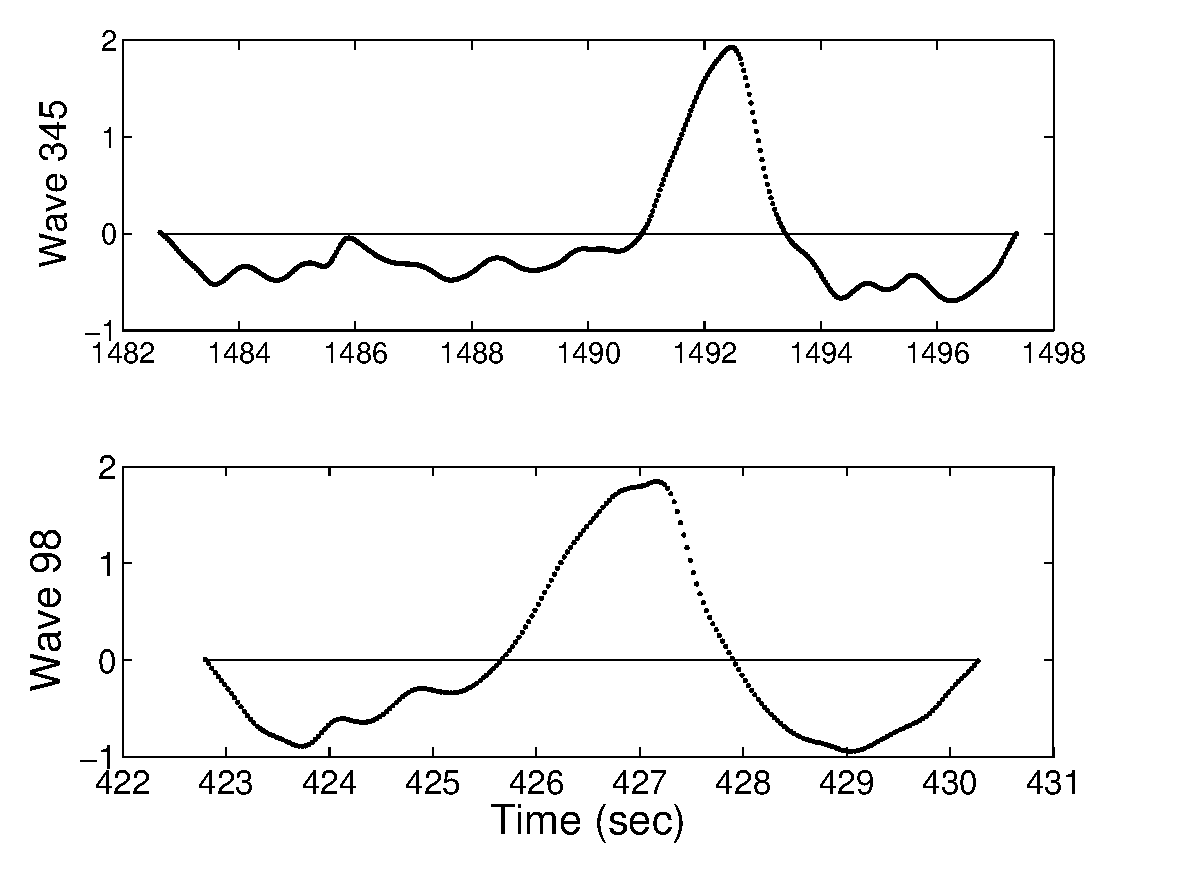
\includegraphics[width=\defwidth]{fig_c_wave}
\end{minipage}}%
\hfill
\subfigure[]{%
\begin{minipage}[b]{0.5\textwidth}%
\centering 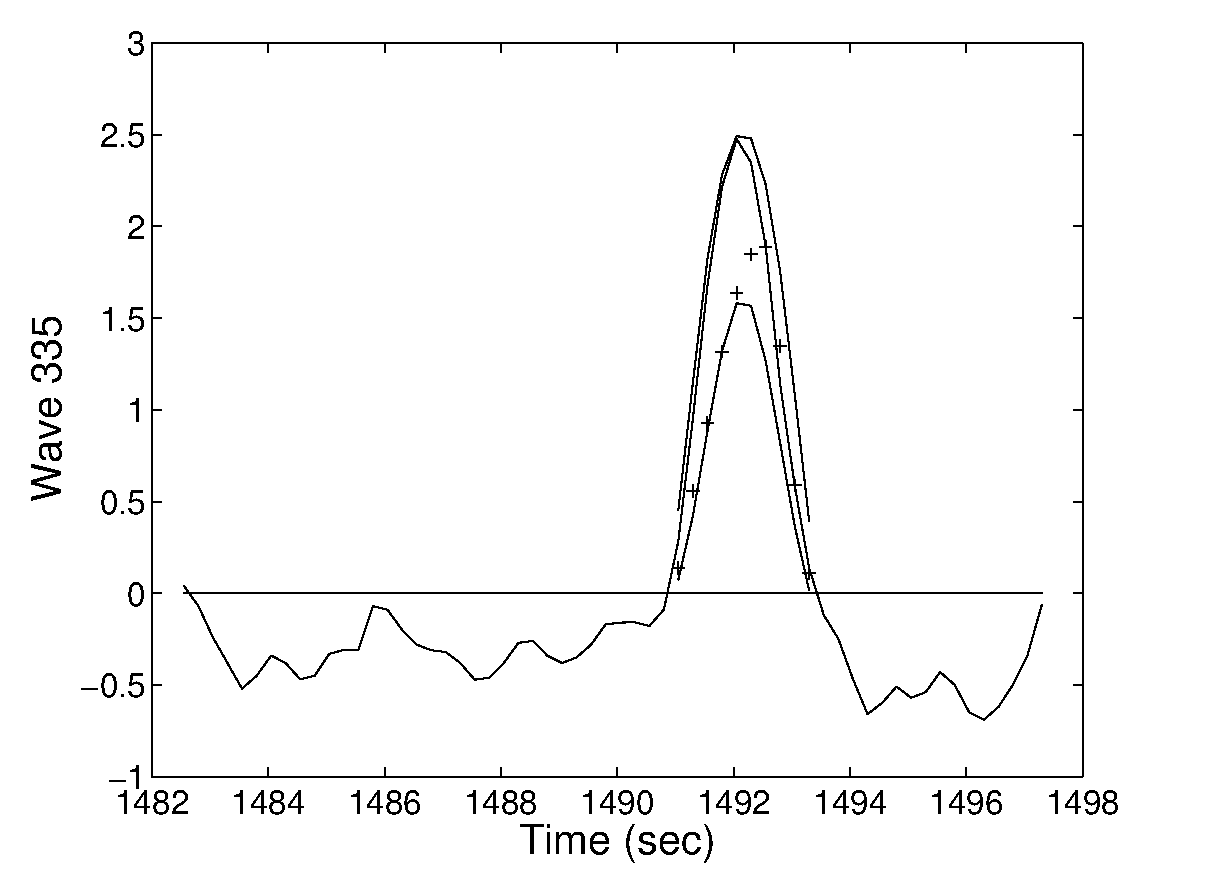
\includegraphics[width=\defwidth]{fig_r_wave}%{Figure33b2017}
\end{minipage}}%
\vspace{-3mm}
  \caption[Reconstructing the highest wave in  {\tt sea.dat}]{
(a): Two waves, the highest and the steepest, observed in {\tt sea.dat}.
(b): Crosses are observations removed from the highest wave.
The reconstructed wave,
using transformed Gaussian model, is given by the middle
solid line. Upper and lower curves give the confidence band defined as the
conditional mean of the process plus minus two conditional standard deviations.
}
\label{fig_c_wave}
\end{figure}

In Figure~\ref{fig_c_wave}(b) the crosses are the removed values from
the wave. The reconstructed wave, plotted by a solid line,
is close to the measured. (Observe that this is a simulated
wave, using the transformed Gaussian model,
and hence each time we execute the command the shape will change.)
The confidence bands gives limits containing 95\% of the simulated
values, pointwise.
From the figure  we can deduce that the highest wave could have been
even higher and that the height is determined by the particularly high
values of the derivatives at the zero crossings which define the wave.
The observed wave looks more asymmetric in time than the reconstructed one.
Such asymmetry is unusual for the transformed Gaussian waves but not
impossible. By executing the following commands we can see that actually the
observed wave is close to the expected in a transformed Gaussian model.
{\small\begin{verbatim}
      plot(xx(inds1,1),xx(inds1,2),'+'), hold on
      mu = tranproc(mu1o,fliplr(grec1));
      plot(y1(inds1,1), mu), hold off
\end{verbatim}}
\noindent
We shall not investigate this question further in this tutorial.
\end{cex}

\subsection{Crest height}
\index[xentr]{wave distributions!estimation of densities!crest height}
We turn now to the kernel estimators of the crest height density.
It is well known that for Gaussian sea the tail of the density is
well approximated by the Rayleigh distribution.
Wand and Jones (1995, Chap. 2.9) show that Gaussian distribution is one
of the easiest distributions to obtain a good Kernel Density Estimate from.
It is more difficult to find good estimates for distributions with
skewness, kurtosis, and multi-modality. Here, one can get help by
transforming data. This can be done choosing different values of input
{\tt L2} into the program {\tt kde}.

\begin{cex}{Ex_sea_statistics}
We shall continue with the analysis of the crest height distribution.
By letting {\tt L2 = 0.6} we see that the normalplot of the transformed data is
approximately linear.
(Note: One should try out several different values for {\tt L2}.
It is also always good practise to try out several different values of
the smoothing parameter; see the help text of {\tt kde} and {\tt kdebin} for
further explanation.)
{\small\begin{verbatim}
      L2 = 0.6;
      plotnorm(Ac.^L2)
      fac = kde(Ac,{'L2',L2},linspace(0.01,3,200));
      pdfplot(fac)
      simpson(fac.x{1},fac.f)
\end{verbatim}}

The integral of the estimated density {\tt fac} is 0.9675 but it should
be one. Therefore, when we use the estimated density to compute different
probabilities concerning the crest height the uncertainty of the computed
probability is at least 0.03. We suspect that this is due to the
estimated density being non-zero for negative values.
In order to check this we compute the
cumulative distribution using the formula,
$$
\pr (Ac\le h)=1-\int_h^{+\infty} f_{Ac}(x)\, \rd x,
$$
where $f_{Ac}(x)$ is the estimated probability density of $Ac$.
For the pdf saved in {\tt fac} the following code gives an estimate of
the cumulative distribution function (cdf) for
crest height and compares it with the empirical distribution
computed from data by means of\index[xcmds]{{\tt plotedf}}
function {\tt edf}\index[xcmds]{{\tt edf}}
or {\tt plotedf}.
{\small\begin{verbatim}
      Fac = flipud(cumtrapz(fac.x{1},flipud(fac.f)));
      Fac = [fac.x{1} 1-Fac];
      Femp = plotedf(Ac,Fac);
      axis([0 2 0 1]), hold off
\end{verbatim}}

Since a kernel density estimator KDE in essence is a smoothed histogram
it is not very well suited for extrapolation of the density to the region
where no data are available, e.g.\ for high crests. In such a case
a parametric model should be used. In \progname{} there is a function
{\tt trraylpdf}\index[xcmds]{{\tt trraylpdf}}
that combines the non-parametric approach of KDE with a Rayleigh density.
Simply, if the Rayleigh variable can be used to described the crests of
Gaussian waves then a transformed Rayleigh variable should be used for
the crests of the transformed Gaussian waves.
The method has several nice properties and will be described more in
Section~\ref{ss:Rayleighappr}. Here we just use it in order to compare with
the non-parametric KDE method.
{\small\begin{verbatim}
      facr = trraylpdf(fac.x{1},'Ac',grec1);
      Facr = cumtrapz(facr.x{1},facr.f); hold on
      plot(facr.x{1},Facr,'.')
      axis([1.25 2.25 0.95 1]), hold off
\end{verbatim}}

Figure \ref{fig_Ac1}(a) shows that our hypothesis that the pdf {\tt fac}
is slightly too low for small crests seems to be correct. Next
from Figure~\ref{fig_Ac1}(b) we can see that also the tail is
reasonably well modelled even if it is lighter than, i.e.\ gives smaller
probabilities of high waves than, the one derived from the transformed
Gaussian model.
\end{cex}

\begin{figure}
\subfigure[]{%
\begin{minipage}[b]{0.5\textwidth}%
\centering 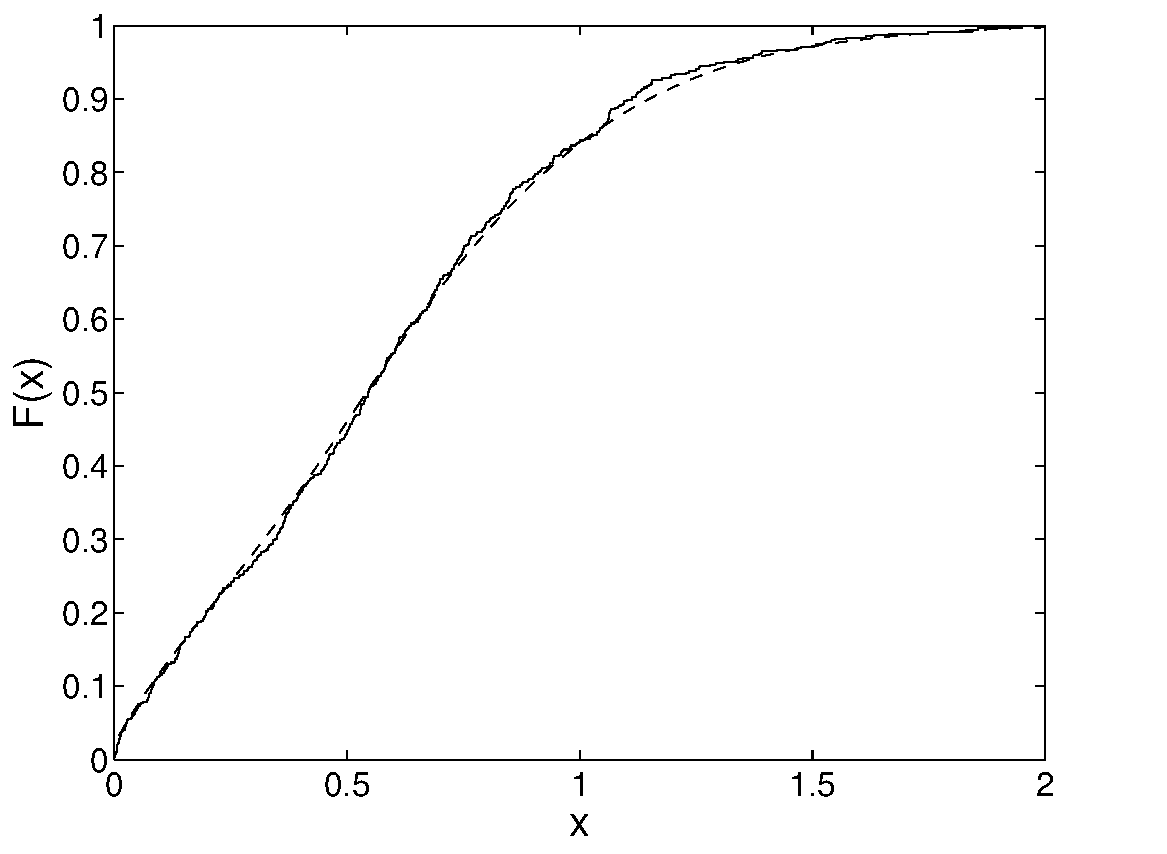
\includegraphics[width=\defwidth]{fig_Ac1}
\end{minipage}}%
\hfill
\subfigure[]{%
\begin{minipage}[b]{0.5\textwidth}%
\centering 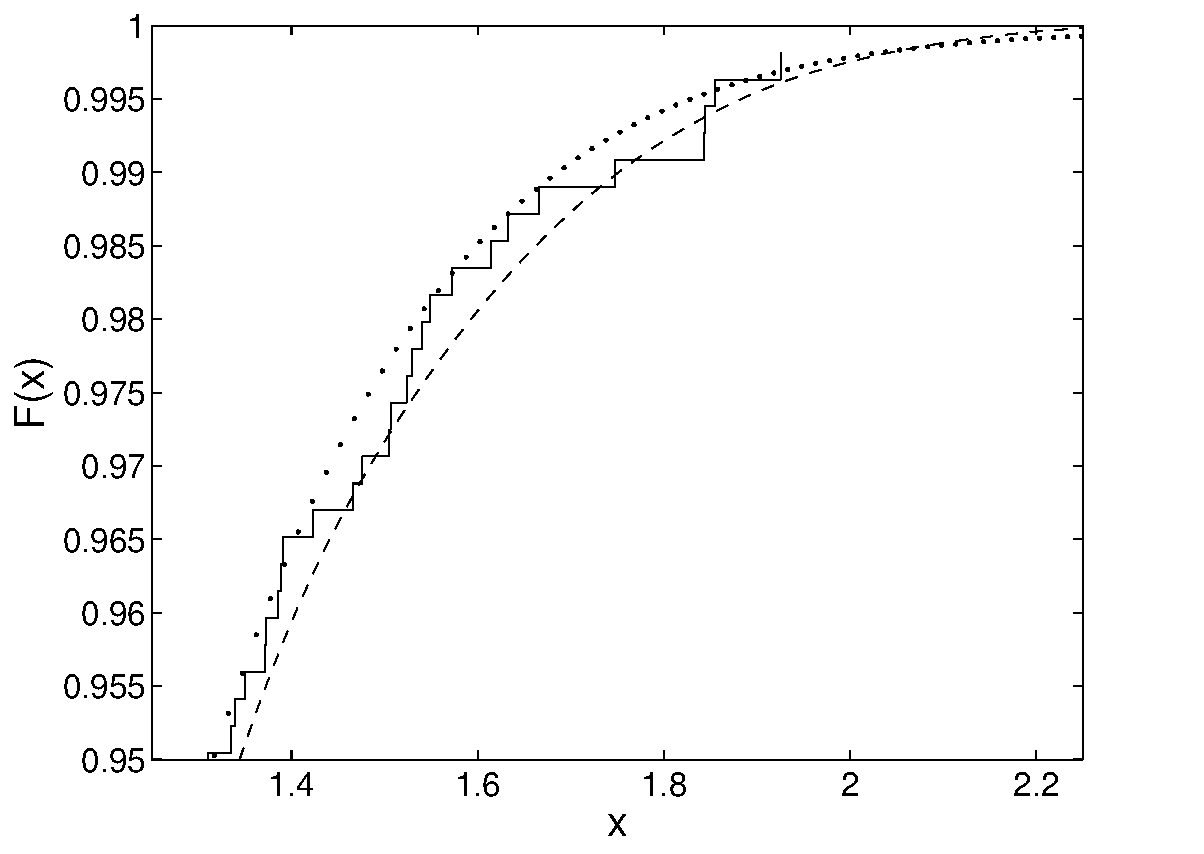
\includegraphics[width=72mm]{fig_Ac2}
\end{minipage}}%
\vspace{-3mm}
  \caption[Comparing different crest height models]{
(a) Comparison of the empirical distribution of the crest height with
the cumulative distribution computed from the KDE estimator.
(b) Zooming in on the tails of distributions in (a) together with
the tail of the transformed Rayleigh approximation (dots) to the crest
height distribution.
}
  \label{fig_Ac1}
\end{figure}

\subsection{Joint crest period and crest height distribution}
\index[xentr]{wave distributions!estimation of densities!
joint crest period and height}
We shall use the kernel density estimator to find a good estimator of
the central part of the joint density of crest period and crest
height. Usually, kernel density estimators give poor estimates
of the tail of the distribution, unless large amounts of data is
available. However, a KDE gives qualitatively good estimates in
regions with sufficient data, i.e.\, in the  main part of the
distribution. This is good for visualization (\verb+pdfplot+) and detecting
modes, symmetries (anti-symmetry) of distributions.

\begin{cex}{Ex_sea_statistics} The following command examines and
  plots the joint distribution of crest period {\tt Tc = Tcf+Tcb}
  and crest height {\tt Ac} in \verb+sea.dat+.
{\small\begin{verbatim}
      kopt2 = kdeoptset('L2',0.5,'inc',256);
      Tc = Tcf+Tcb;
      fTcAc = kdebin([Tc Ac],kopt2);
      fTcAc.labx={'Tc [s]'  'Ac [m]'} % make labels for the plot
      pdfplot(fTcAc), hold on
      plot(Tc,Ac,'k.'), hold off
\end{verbatim}}

\begin{figure}
\centering
   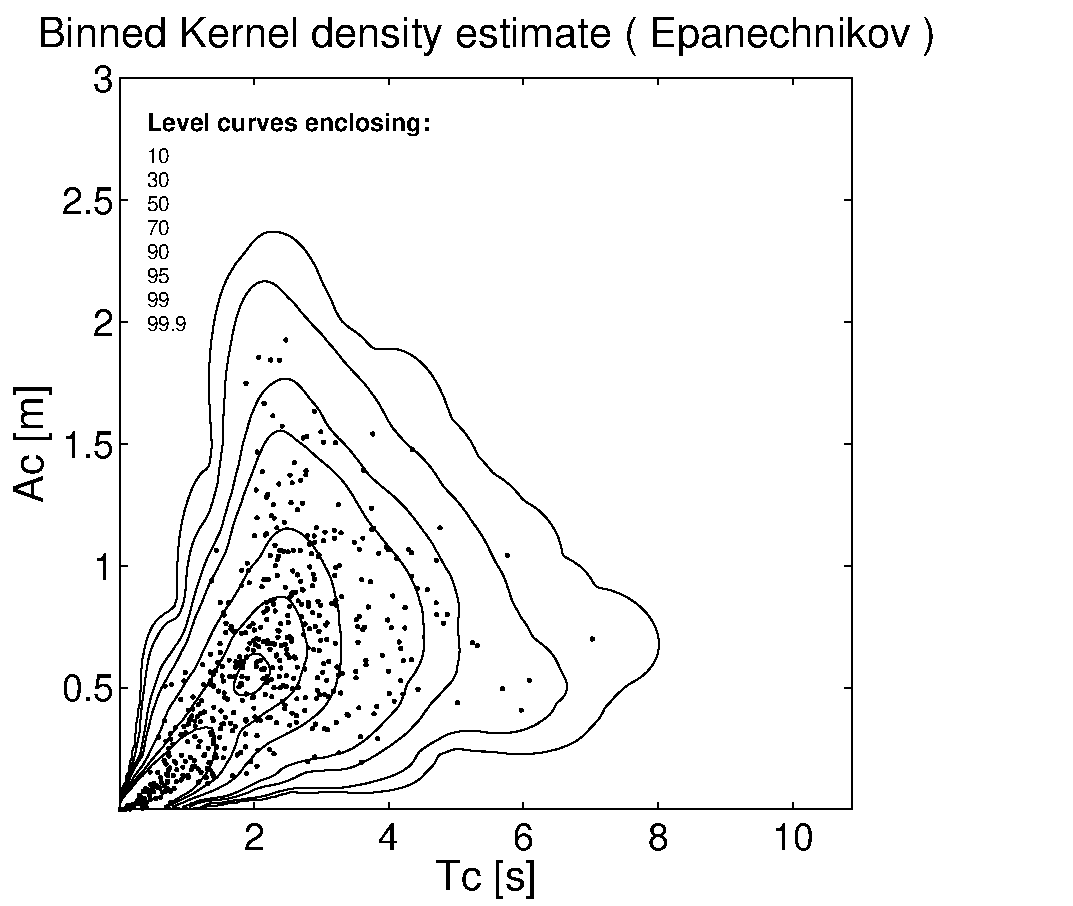
\includegraphics[width=\narrowfigwidth]{fig_TcAc}
\vspace{-3mm}
  \caption[Kernel estimate of the joint density of crest period and
crest height]{
Kernel estimate of joint density of crest period {\tt Tc} and
crest height {\tt Ac} in {\tt sea.dat} compared with the observed data
(dots). The contour lines are drawn in such a way that they contain
specified (estimated) proportions of data.
}
  \label{fig_TcAc}
\end{figure}

In Figure~\ref{fig_TcAc} are plotted 544 pairs of crest period and
height. We can see that the kernel estimate describes the
distribution of data quite well. It is also obvious that it can not be
used to extrapolate outside the observation range. In the following
chapter we shall compute the theoretical joint density of crest period
and height from the transformed Gaussian model and compare with the
KDE estimate.
\end{cex}\index[xentr]{wave characteristics!estimation from data|)}

\section{Explicit results - parametric wave models}
\label{sec:explicitresults_wavemodels}
\index[xentr]{wave models|(}

In this section we shall consider the Gaussian sea with well-defined spectrum. We assume that the
reference level is zero. We will
present some explicit results that are known and
studied in the literature about wave characteristics. Some of them are
exact, others are derived by simplification of the random functions
describing the sea surface.

\subsection{The average wave}
For Gaussian waves the spectrum and the spectral moments contain exact
information about the average behaviour of many wave
characteristics. The \progname{} routines
\verb+spec2char+\index[xcmds]{{\tt spec2char}} and
\verb+spec2bw +\index[xcmds]{{\tt spec2bw}}
compute a long list of wave characteristic parameters.


\begin{rtex}{Ex_wave_parameters}{Simple wave characteristics obtained
    from spectral density}
We start by defining a {\sc Jonswap} spectrum, describing a sea state with
$T_p = 10$ [s], $H_{m_0} = 5$ [m]. Type \verb+spec2mom+ to see what
spectral moments are computed. \index[xcmds]{{\tt spec2mom}}
{\small\begin{verbatim}
     SJ = jonswap([],[5 10]);
     [m mt]= spec2mom(SJ,4,[],0);
\end{verbatim}}

The most basic information about waves is contained
in the spectral moments. The variable {\tt mt} now contains information
about what kind of moments have been computed, in this case spectral
moments up to order four ($m_0, \ldots , m_4$). Next, the irregularity
factor $\alpha$, significant wave height, zero crossing wave period,
and peak period can be computed.
{\small\begin{verbatim}
      spec2bw(SJ)
      [ch Sa2] = spec2char(SJ,[1  3])
\end{verbatim}}

The interesting feature of the  program {\tt spec2char} is that it
also computes an estimate of the variance of the characteristics, given
the length of observations (assuming the Gaussian sea); see
\cite{KrogstadEtal1999Methods}, \cite{Tucker1993recommended}, %,Tu93}
and \cite{Young1999Wind} %,Yo99}
for more detailed
discussion. For example, for the {\sc Jonswap} Gaussian sea,
the standard deviation of significant wave height estimated from 20 minutes
of observations is approximately 0.25~meter.
\end{rtex}

\subsection{Explicit approximations of wave distributions}
\label{sec:explicit_approximations}
\index[xentr]{crest densities|see wave distributions}

\index[xcmds]{{\tt wavemodels}}
\index[xcmds]{{\tt perioddef}}
\index[xcmds]{{\tt ampdef}}
In the module {\tt wavemodels}, we have implemented some of
the approximative models that have been suggested in the literature.
To get an overview of the routines in the module, use the help function on
{\tt wavemodels}.

We will investigate two suggested approximations for the joint pdf of
{\tt (Tc,Ac)}; for the nomenclature, see the routines {\tt perioddef} and
{\tt ampdef} in the module {\tt docs}. Both  functions
need spectral moments as inputs. One should bear in mind that the
models only depend on a few spectral moments and not
on the full wave spectrum.

\subsubsection*{Model by Longuet-Higgins}  %------------
% Parametrization as in Srokosz and Challenor
\index[xentr]{wave models!Longuet-Higgins}
\index[xentr]{wave distributions!approximative densities!
Longuet-Higgins}
Longuet-Higgins,
\cite{Longuet-Higgins1975Joint,Longuet-Higgins1983Joint}, derived his
approximative distribution by considering the joint
distribution of the envelope amplitude and the time derivative of the
envelope phase. The model is valid for narrow-band processes.
It seams to give relatively accurate results for big waves, e.g.\
for waves with significant amplitudes.

The Longuet-Higgins density depends, besides
the significant wave height $H_s$ and peak period $T_p$, on
the spectral width parameter
$ \nu = \frac{m_0m_2}{m_1^2}-1$,
which can be calculated by the command {\tt spec2bw(S,'eps2')},
(for a narrow-band process, $\nu \approx 0$). The explicit density is
given by
\[
f^{\mbox{\scriptsize{LH}}}_{T_c,A_c}(t,x)=c_{\mbox{\scriptsize{LH}}}\,
\left(\frac{x}{t}\right)^2 \exp\left\{
    -\frac{x^2}{8}\big[1+\nu^{-2}(1-t^{-1})^2\big] \right\} ,
\]
where
\[
c_{\mbox{\scriptsize{LH}}}=\frac{1}{8}(2\pi)^{-1/2}\nu^{-1}[
  1+(1+\nu^2)^{-1/2}]^{-1}.
\]
The density is calculated by the
function \verb+lh83pdf+. \index[xcmds]{{\tt lh83pdf}}

\begin{cex}{Ex_wave_parameters} For the Longuet-Higgins approximation of the 
$T_c,A_c$ distribution for {\sc Jonswap} waves we use the spectral moments just calculated.
{\small\begin{verbatim}
      t = linspace(0,15,100);
      h = linspace(0,6,100);
      flh = lh83pdf(t,h,[m(1),m(2),m(3)]);
\end{verbatim}}

%%%%%%%%%%%%%% Figure L-H %%%%%%%%%%%%%%%%%%%%%%%

\begin{figure}
\subfigure[]{%
\begin{minipage}[b]{0.5\textwidth}%
\centering 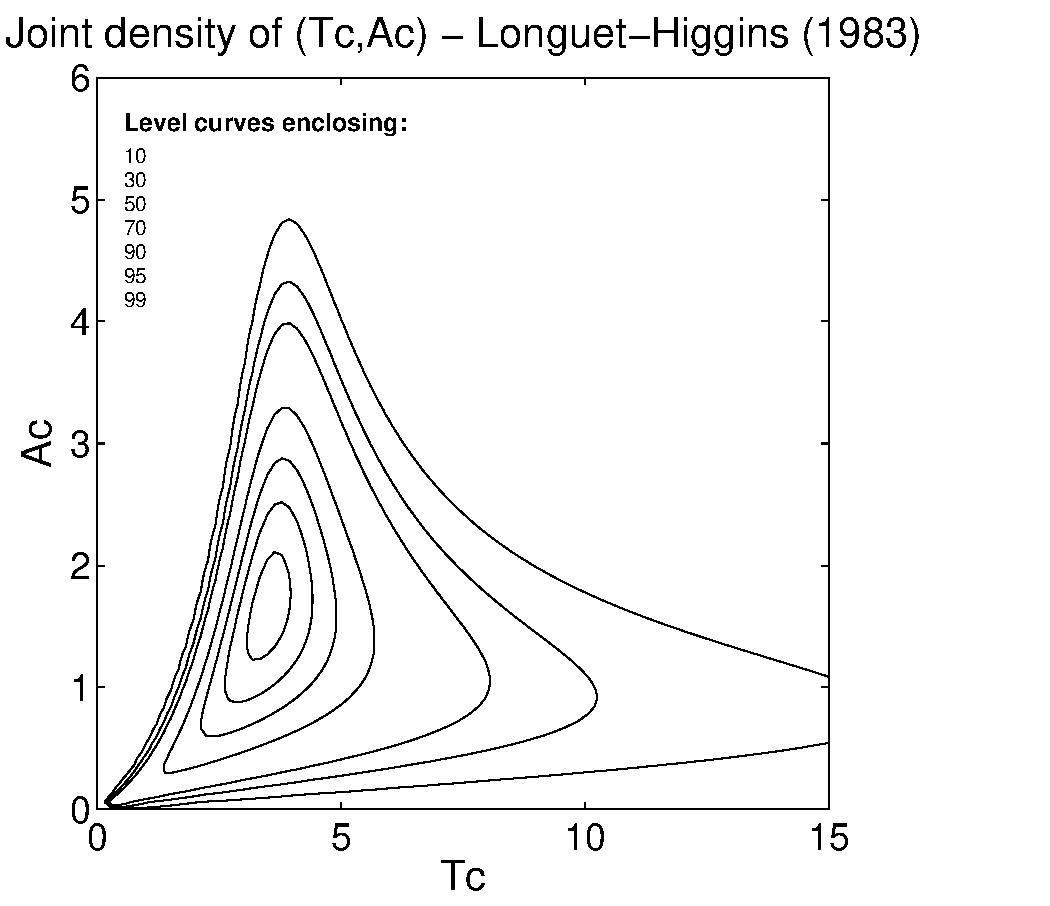
\includegraphics[width=\defwidth]{lhdens}
\end{minipage}}%
\hfill
\subfigure[]{%
\begin{minipage}[b]{0.5\textwidth}%
\centering 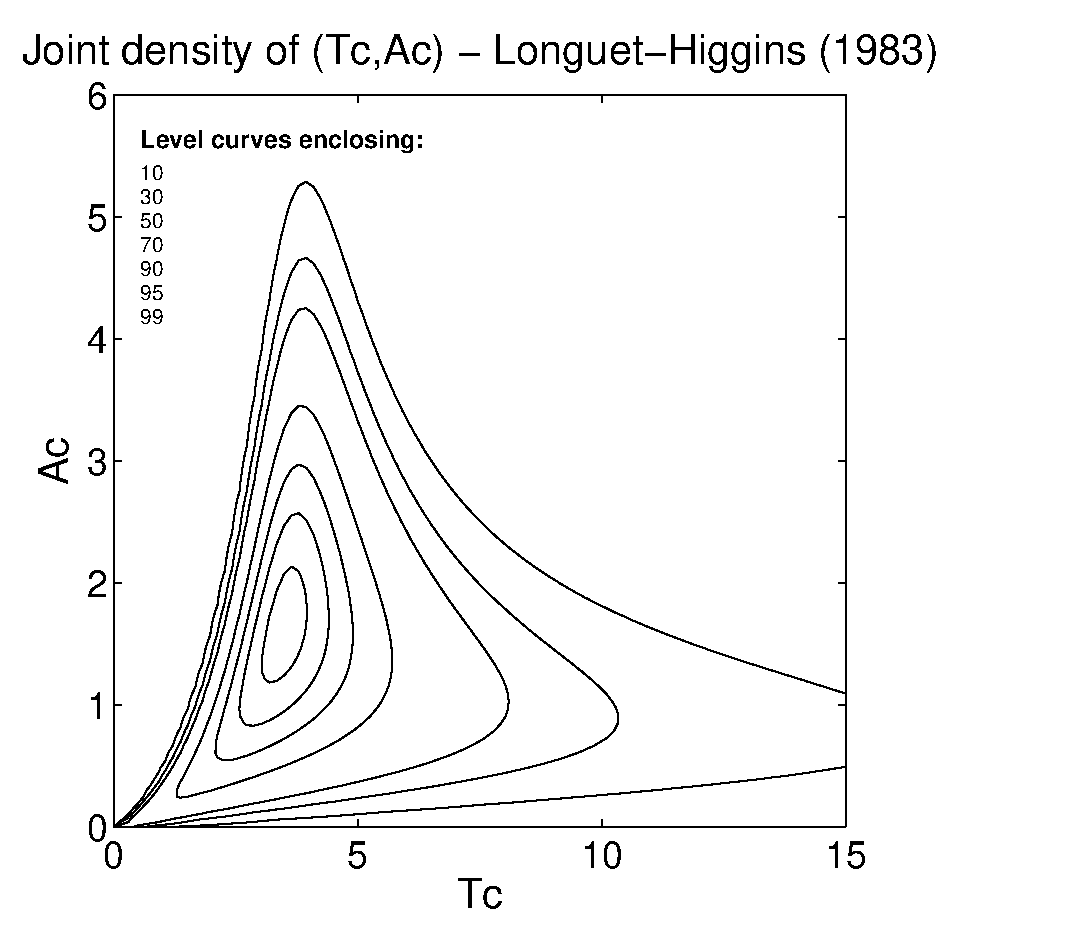
\includegraphics[width=\defwidth]{lhdens1}
\end{minipage}}
\vspace{-3mm}
  \caption[Longuet-Higgins model for joint pdf of crest period and height]{%
Longuet-Higgins model for joint pdf of crest period $T_c$
and crest height $A_c$. Spectrum: JONSWAP with $T_p=10$~[s], $H_{m_0}=5$~[m].
(a) linear Gaussian sea, (b) transformed Gaussian sea.
}
\label{fig:lhdens}
\end{figure}

In \progname{} we have modified the Longuet-Higgins
density to be applicable also for
transformed Gaussian models. Following the examples from the previous chapter
we compute the transformation proposed by Winterstein and combine it with
the Longuet-Higgins model.
{\small\begin{verbatim}
      [sk, ku] = spec2skew(SJ);
      sa = sqrt(m(1));
      gh = hermitetr([],[sa sk ku 0]);
      flhg = lh83pdf(t,h,[m(1),m(2),m(3)],gh);
\end{verbatim}} \index[xcmds]{{\tt spec2skew}}\index[xcmds]{{\tt hermitetr}}

In Figure~\ref{fig:lhdens} the densities {\tt flh} and {\tt flhg} are
compared. The contour lines are drawn in such a way that they contain
predefined proportions of the total probability mass inside the
contours. We can see that including some nonlinear effects
gives somewhat higher waves for the {\sc Jonswap} spectrum.
\end{cex}

 %%%%%%%%%%%%%%%%%%%%%%%%%%%%%%%%%%%%%%%%%%%%
\subsubsection*{Model by Cavani\'e et al.} %------------
% Parametrization as in Srokosz and Challenor!
\index[xentr]{wave models!Cavani\'e et al.}
\index[xentr]{wave distributions!approximative densities!
Cavani\'e et al.}
Another explicit density for the crest height was proposed
by Cavani{\' e} et al., \cite{CavanieEtal1976Statistical}.
Here any positive local maximum is considered
as a crest of a wave, and then the second derivative (curvature) at the
local maximum defines the wave period as if the entire wave was a cosine function
with the same height and the same crest curvature.

The model uses the parameter $\nu$  and a higher order bandwidth
parameter\footnote{The value of $\epsilon$ may be
  calculated by {\tt spec2bw(S,'eps4')}}
$\epsilon$, defined by
\begin{align*}
\epsilon &= \sqrt{1-\frac{m_2^2}{m_0m_4}};
\end{align*}
where, for a narrow-band process, $\epsilon \approx 0$. The
  Cavani{\'e} distribution is given by
\begin{align*}
f^{\mbox{\scriptsize{CA}}}_{T_c,A_c}(t,x) &=
c_{\mbox{\scriptsize{CA}}}
\frac{x^2}{t^5}\exp \left \{-\frac{x^2}{8\varepsilon^2 t^4}\left[
\left( t^2-\left(\frac{1-\varepsilon^2}{1+\nu^2}\right)\right)^2+
\beta^2\left(\frac{1-\varepsilon^2}{1+\nu^2}\right)\right]\right\},
\intertext{where}
c_{\mbox{\scriptsize{CA}}} &=
  \frac{1}{4}(1-\epsilon^2)(2\pi)^{-1/2}{\epsilon}^{-1}
             {\alpha_2}^{-1}(1+\nu^2)^{-2}, \\
  {\alpha}_2 &= \frac{1}{2}[1+(1-{\epsilon}^2)^{1/2}], \\
  \beta &= {\epsilon}^2/(1-{\epsilon}^2) .
  \end{align*}
The density is computed by
{\small\begin{verbatim}
      t = linspace(0,10,100);
      h = linspace(0,7,100);
      fcav = cav76pdf(t,h,[m(1) m(2) m(3) m(5)],[]);
\end{verbatim}}\index[xcmds]{{\tt cav76pdf}}

\noindent
and a contour plot of the pdf is obtained by {\tt pdfplot(fcav)};
see~Figure~\ref{fig:cavdens}.

%%%%%%%%%%%%%%%%%%%%%%%%%%%%%% Figure Cavanie %%%%%%%%%%%
\begin{figure}
\subfigure[]{%
\begin{minipage}[b]{0.45\textwidth}%
\centering
%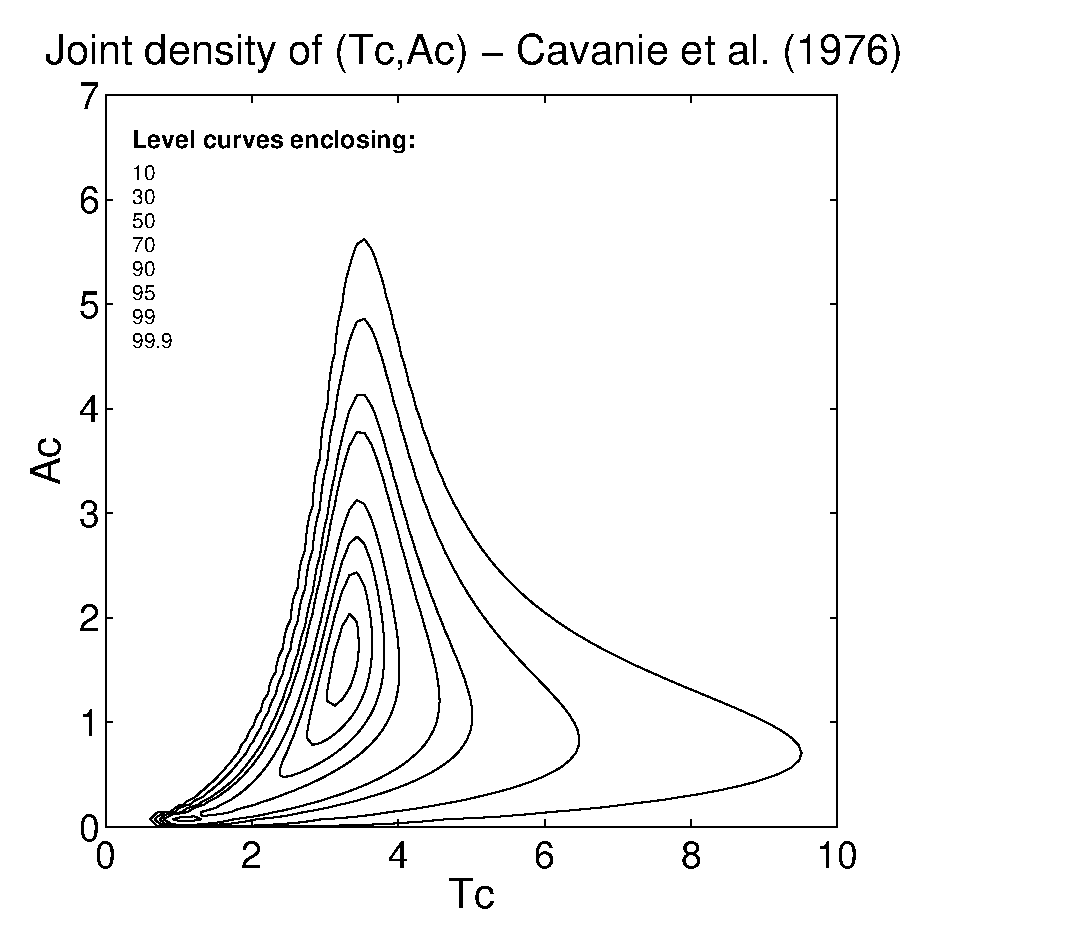
\includegraphics[height=\defheight]{cavdens}
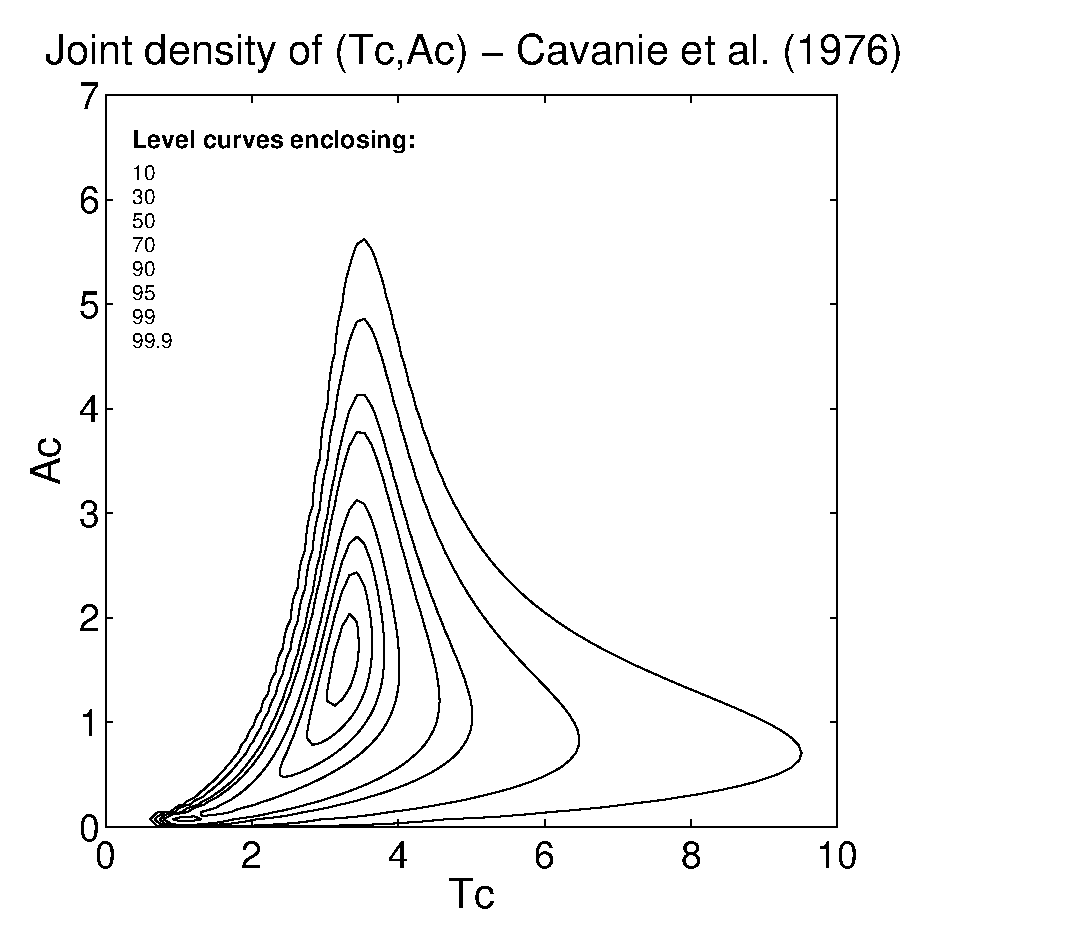
\includegraphics[height=58mm]{cavdens}
\end{minipage}}%
\hspace{0mm}
%\hfill
\subfigure[]{%
\begin{minipage}[b]{0.54\textwidth}%
\centering
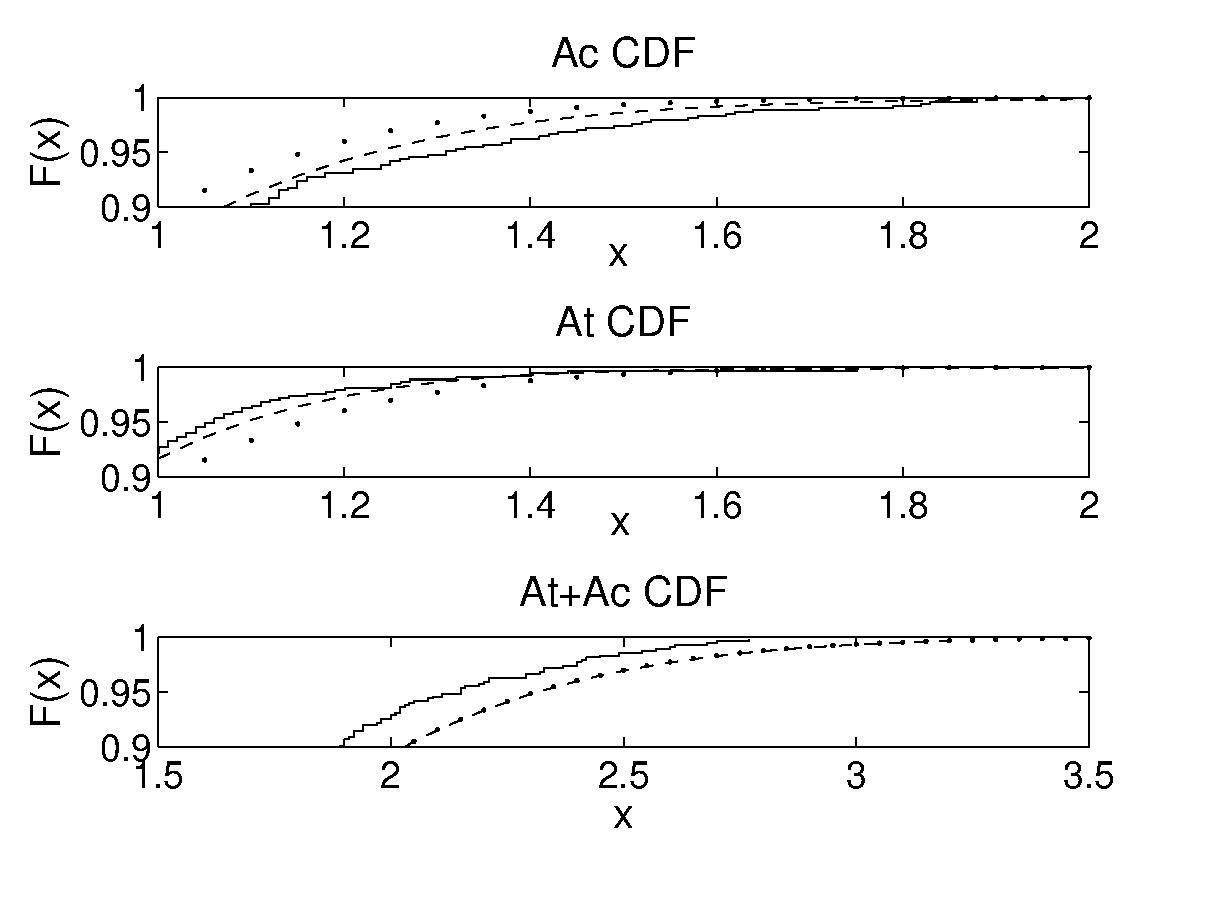
\includegraphics[height=58mm]{figAcAt_h}
\end{minipage}}
\vspace{-3mm}
  \caption[Joint density of crest period and
crest height by Cavani\'e et al]{
(a) Contour lines of the joint density of crest period and
crest height proposed by Cavani\'e et al, for Gaussian sea with
{\sc Jonswap} spectrum ($T_p=10$ [s], $H_{m_0}=5$ [m]). (b) The tail of the
empirical distribution of crest height (top), trough depth (middle) and
amplitude (bottom) compared with Rayleigh approximation (dots) and
transformed Rayleigh model with Hermite transformation.
}
  \label{fig:cavdens}
\end{figure}
%%%%%%%%%%%%%%%%%%%%%%%%%%%%%%%%%%%%%%%%%%%%%%%%%%%%%

\subsection{Rayleigh approximation for wave crest height}\label{ss:Rayleighappr}
\index[xentr]{wave distributions!approximative densities!
Rayleigh approximation}\label{ss:Rayleighapproximation}
There are several densities proposed in the literature to approximate
the height of a wave crest or its amplitude. Some of them are programmed
in \progname{}; execute {\tt help wavemodels} for a list.
For Gaussian sea the most simple and most
frequently used model is the Rayleigh
density. The standardized Rayleigh variable $R$ has probability density 
$f(r)=r\exp(-r^2/2)$, $x > 0$. It is well known that for Gaussian sea
the Rayleigh approximation works very well for high waves,
and actually it is a conservative approximation since we have
$$
\pr (A_c > h) \leq \pr (R> 4 h/H_s) = e^{-8h^2/H_s^2},
$$
see \cite{RyclikAndLeadbettter1997Analysis}.
In that paper it is also shown that for any sea wave model with
crossing intensity $\mu(u)$, one has $\pr (A_c>h) \leq \mu(u)/\mu(0)$.
The approximation becomes more accurate as the level $h$
increases.

The crossing intensity $\mu(u)$ is given by
Rice's formula, Rice (1944),\index[xentr]{Rice's formula}
\index[xentr]{crossing intensity!Rice's formula}
and it can be computed when the joint density of sea level $X(t)$ and its
derivative $X'(t)$ is known, see Section~\ref{subsec:crossing_intensity},
$$
\mu(u) = \int_0^{\infty} zf_{X(t), X'(t)}(u,z)\,\rd z.
$$
For a Gaussian sea it can be computed explicitly,
$$
\mu(u) = \frac{1}{T_z} e^{-8u^2/H_s^2}.
$$
For non-linear wave models with random Stokes waves the crossing
intensity has to be computed using numerical integration; see the
work  by Machado and Rychlik,
\cite{MachadoAndRychlik2003Wave}.

Knowing the crossing intensity $\mu(u)$ one can compute the
transformation $g$, by using the routine
{\tt lc2tr}\index[xcmds]{{\tt lc2tr}}, such that  the transformed
Gaussian model has crossing intensity equal to $\mu(u)$. Consequently,
we have that \index[xcmds]{{\tt ls2tr}}
$
\pr (A_c>h) \leq \pr (R> g(h)) = 1- \pr (G(R)\leq h).$
The function {\tt trraylpdf} computes the pdf of $G(R)$. (Obviously
the function works for any transformation $g$.)
\index[xcmds]{{\tt trraylpdf}}

In previous examples we used the estimated crossing intensity to
compute the transformation and then approximated the crest height
density using the transformed Rayleigh variable.
The accuracy of the approximation for the high crests in
the data set {\tt xx = sea.dat} was checked, see Figure~\ref{fig_Ac1}(b).
A more extensive study of the applicability of this approximation
is done in \cite{RyclikAndLeadbettter1997Analysis}.


\begin{rtex}{rayleighapproximation}{Rayleigh approximation of crest
height from spectral density}
In this example we shall use a transformed Rayleigh approximation for
crest height derived from a sea spectrum. In order to check the
accuracy of the approximations we shall use the estimated spectrum
from the record {\tt sea.dat}.
{\small\begin{verbatim}
      xx = load('sea.dat');
      x = xx;
      x(:,2) = detrend(x(:,2));
      SS = dat2spec2(x);
      [sk, ku, me, si] = spec2skew(SS);
      gh = hermitetr([],[si sk ku me]);
      Hs = 4*si;
      r = (0:0.05:1.1*Hs)';
      fac_h = trraylpdf(r,'Ac',gh);
      fat_h = trraylpdf(r,'At',gh);
      h = (0:0.05:1.7*Hs)';
      facat_h = trraylpdf(h,'AcAt',gh);
      pdfplot(fac_h), hold on
      pdfplot(fat_h), hold off
\end{verbatim}}

Next, we shall compare the derived approximation with the observed
crest heights in {\tt x}. As before, we could use the function {\tt dat2steep}
to find the crests. Here, for illustration only,  we shall use
{\tt dat2tc}\index[xcmds]{{\tt dat2tc}}
to find the crest heights {\tt Ac} and trough depth {\tt At}.
{\small\begin{verbatim}
      TC = dat2tc(xx, me);
      tc = tp2mm(TC);
      Ac = tc(:,2); At = -tc(:,1);
      AcAt = Ac+At;
\end{verbatim}}

Finally, the following commands will give the cumulative distributions
for the computed densities.
{\small\begin{verbatim}
      Fac_h = [fac_h.x{1} cumtrapz(fac_h.x{1},fac_h.f)];
      subplot(3,1,1)
      Fac = plotedf(Ac,Fac_h); hold on
      plot(r,1-exp(-8*r.^2/Hs^2),'.')
      axis([1. 2. 0.9 1])
      Fat_h = [fat_h.x{1} cumtrapz(fat_h.x{1},fat_h.f)];
      subplot(3,1,2)
      Fat = plotedf(At,Fat_h); hold on
      plot(r,1-exp(-8*r.^2/Hs^2),'.')
      axis([1. 2. 0.9 1])
      Facat_h = [facat_h.x{1} cumtrapz(facat_h.x{1},facat_h.f)];
      subplot(3,1,3)
      Facat = plotedf(AcAt,Facat_h); hold on
      r2 = (0:05:2.1*Hs)';
      plot(r2,1-exp(-2*r2.^2/Hs^2),'.')
      axis([1.5 3.5 0.9 1]), hold off
\end{verbatim}}

In Figure~\ref{fig:cavdens}(b) we can see some differences between the
observed crest and trough distributions and those obtained from the
transformation {\tt gh}.  However, it still gives a much better
approximation than the standard Rayleigh approximation (dots).
As it was shown before, using the transformation computed from the
crossing intensity, the transformed Rayleigh approach is giving
a perfect fit. Finally, one can see that the Rayleigh and transformed
Rayleigh variables give too conservative approximations to
the distribution of wave amplitude.
\end{rtex}\index[xentr]{wave models|)}

%\begin{comment}
\newpage
\section{\progname{} wave characteristics}\label{sec:WAFOcharacteristics}

\subsection{spec2char}\label{ss:spectralcharacteristics}
\index[xentr]{wave characteristics!computation from spectrum}
{\small\begin{verbatim}
help spec2char

 SPEC2CHAR Evaluates spectral characteristics and their variance

 CALL: [ch r chtext] = spec2char(S,fact,T)

       ch = vector of spectral characteristics
       r  = vector of the corresponding variances given T
   chtext = a cellvector of strings describing the elements of ch
       S  = spectral struct with angular frequency
     fact = vector with factor integers, see below.
            (default [1])
       T  = recording time (sec) (default 1200 sec = 20 min)

 If input spectrum is of wave number type, output are factors
 for corresponding 'k1D', else output are factors for 'freq'.
 Input vector 'factors' correspondence:
    1 Hm0   = 4*sqrt(m0)           Significant wave height
    2 Tm01  = 2*pi*m0/m1           Mean wave period
    3 Tm02  = 2*pi*sqrt(m0/m2)     Mean zero-crossing period
    4 Tm24  = 2*pi*sqrt(m2/m4)     Mean period between maxima
    5 Tm_10 = 2*pi*m_1/m0          Energy period
    6 Tp    = 2*pi/{w | max(S(w))} Peak period
    7 Ss    = 2*pi*Hm0/(g*Tm02^2)  Significant wave steepness
    8 Sp    = 2*pi*Hm0/(g*Tp^2)    Average wave steepness
    9 Ka    = abs(int S(w) exp(i*w*Tm02) dw) / m0
                                   Groupiness parameter
   10 Rs    = se help spec2char    Quality control parameter
   11 Tp    = 2*pi*int S(w)^4 dw   Peak Period
              ------------------   (more robust estimate)
              int w*S(w)^4 dw

   12 alpha = m2/sqrt(m0*m4)       Irregularity factor
   13 eps2  = sqrt(m0*m2/m1^2-1)   Narrowness factor
   14 eps4  = sqrt(1-m2^2/(m0*m4)) = sqrt(1-alpha^2)  Broadness factor
   15 Qp    = (2/m0^2)int_0^inf w*S(w)^2 dw           Peakedness factor

 Order of output is same as order in 'factors'
 The variances are computed with a Taylor expansion technique
 and is currently only available for factors 1,2 and 3.
\end{verbatim}}\index[xcmds]{{\tt spec2char}}

\newpage
\subsection{spec2bw}
{\small\begin{verbatim}
help spec2bw

 SPEC2BW Evaluates some spectral bandwidth and irregularity factors

  CALL:  bw = spec2bw(S,factors)

         bw = vector of factors
         S  = spectrum struct
    factors = vector with integers, see below. (default [1])

  If input spectrum is of wave-number type, output are factors for
  corresponding 'k1D', else output are factors for 'freq'.
  Input vector 'factors' correspondence:
     1 alpha=m2/sqrt(m0*m4)                        (irregularity factor)
     2 eps2 = sqrt(m0*m2/m1^2-1)                   (narrowness factor)
     3 eps4 = sqrt(1-m2^2/(m0*m4))=sqrt(1-alpha^2) (broadness factor)
     4 Qp=(2/m0^2)int_0^inf f*S(f)^2 df            (peakedness factor)
  Order of output is the same as order in 'factors'

  Example:
    S=demospec;
    bw=spec2bw(S,[1 2 3 4]);
\end{verbatim}} \index[xcmds]{{\tt spec2bw}}

\newpage
\subsection{wavedef}\index[xentr]{wave characteristics!definitions}
{\small\begin{verbatim}
help wavedef

  WAVEDEF wave definitions and nomenclature

  Definition of trough and crest:
 ~~~~~~~~~~~~~~~~~~~~~~~~~~~~~~~~
  A trough (t) is defined as the global minimum between a
  level v down-crossing (d) and the next up-crossing (u)
  and a crest (c) is defined as the global maximum between
  a level v up-crossing and the following down-crossing.

  Definition of down- and up-crossing waves:
 ~~~~~~~~~~~~~~~~~~~~~~~~~~~~~~~~~~~~~~~~~~~~~
  A level v-down-crossing wave (dw) is a wave from a
  down-crossing to the following down-crossing.
  Similarly a level v-up-crossing wave (uw) is a wave from
  an up-crossing to the next up-crossing.

  Definition of trough and crest waves:
 ~~~~~~~~~~~~~~~~~~~~~~~~~~~~~~~~~~~~~~
  A trough to trough wave (tw) is a wave from a trough (t)
  to the following trough.
  The crest to crest wave (cw) is defined similarly.

  Definition of min2min and Max2Max wave:
 ~~~~~~~~~~~~~~~~~~~~~~~~~~~~~~~~~~~~~~~~~
  A min2min wave (mw) is defined starting from a minimum (m)
  and ending in the following minimum.
  A Max2Max wave (Mw) is a wave from a maximum (M) to
  the next maximum (all waves optionally rainflow filtered).

            <----- Direction of wave propagation
    <------Mw-----> <----mw---->
    M             : :  c       :
   / \            M : / \_     :     c_            c
  F   \          / \m/    \    :    /: \          /:\   level v
 ------d--------u----------d-------u----d--------u---d--------
        \      /:           \  :  /: :  :\_    _/  : :\_   L
         \_   / :            \_t_/ : :  :  \t_/    : :  \m/
           \t/  <-------uw---------> :  <-----dw----->
            :                  :     :             :
            <--------tw-------->     <------cw----->
  (F= first value and L=last value).
 See also: tpdef, crossdef, dat2tc, dat2wa, dat2crossind
\end{verbatim}
}\index[xcmds]{{\tt wavedef}}

\newpage
\subsection{perioddef}
{\small\begin{verbatim}
help perioddef

  PERIODDEF wave periods (lengths) definitions and
  nomenclature

  Definition of wave periods (lengths):
 ---------------------------------------

            <----- Direction of wave propagation

                <-------Tu-------->
                :                 :
                <---Tc----->      :
                :          :      : <------Tcc---->
    M           :      c   :      : :             :
   / \          : M   / \_ :      : c_            c
  F   \         :/ \m/    \:      :/  \          / \   level v
 ------d--------u----------d------u----d--------u---d--------
        \      /            \    /     :\_    _/:   :\_   L
         \_   /              \t_/      :  \t_/  :   :  \m/
           \t/                :        :        :   :
            :<-------Ttt----->:        <---Tt--->   :
                                       :<----Td---->:
   Tu   = Wave up-crossing period
   Td   = Wave down-crossing period
   Tc   = Crest period, i.e., period between up-crossing and
          the next down-crossing
   Tt   = Trough period, i.e., period between down-crossing and
          the next up-crossing
   Ttt  = Trough2trough period
   Tcc  = Crest2crest period
\end{verbatim}
}\index[xcmds]{{\tt perioddef}}

\newpage
{\small\begin{verbatim}
            <----- Direction of wave propagation

                 <--Tcf->                           Tuc
                 :      :               <-Tcb->     <->
    M            :      c               :     :     : :
   / \           : M   / \_             c_    :     : c
  F   \          :/ \m/    \           /  \___:     :/ \ level v
 ------d---------u----------d---------u-------d-----u---d-------
       :\_      /            \     __/:        \   /     \_   L
       :  \_   /              \_t_/   :         \t/        \m/
       :    \t/                 :     :
       :     :                  :     :
       <-Ttf->                  <-Ttb->

   Tcf  = Crest front period, i.e., period between up-crossing
          and crest
   Tcb  = Crest back period, i.e., period between crest and
          down-crossing
   Ttf  = Trough front period, i.e., period between
          down-crossing and trough
   Ttb  = Trough back period, i.e., period between trough and
          up-crossing

  Also note that Tcf and Ttf can also be abbreviated by their
  crossing marker, e.g. Tuc (u2c) and Tdt (d2t), respectively.
  Similar rules apply to all the other wave periods and wave
  lengths. (The nomenclature for wave length is similar, just
  substitute T and period with L and length, respectively)

              <----- Direction of wave propagation
                       <--TMm-->
            <-TmM->    :       :
    M       :     :    M       :
   / \      :     M   /:\_     :     M_            M
  F   \     :    / \m/ :  \    :    /: \          / \
       \    :   /      :   \   :   / :  \        /   \
        \   :  /       :    \  :  /  :   \_    _/     \_   L
         \_ : /        :     \_m_/   :     \m_/         \m/
           \m/         :             :      :            :
                       <-----TMM----->      <----Tmm----->

   TmM = Period between minimum and the following Maximum
   TMm = Period between Maximum and the following minimum
   TMM = Period between Maximum and the following Maximum
   Tmm = Period between minimum and the following minimum
See also: wavedef, ampdef, crossdef, tpdef
\end{verbatim}
  }

%\newpage
\subsection{ampdef}
{\small\begin{verbatim}
help ampdef

  AMPDEF wave heights and amplitude definitions and
  nomenclature

  Definition of wave amplitude and wave heights:
 ~~~~~~~~~~~~~~~~~~~~~~~~~~~~~~~~~~~~~~~~~~~~~~~

             <----- Direction of wave propagation

            ...............c_..........
            |             /| \         |
        Hd  |           _/ |  \        |  Hu
    M       |          /   |   \       |
   / \      |     M   / Ac |    \_     |     c_
  F   \     |    / \m/     |      \    |    /  \  level v
 ------d----|---u------------------d---|---u----d------
        \   |  /|                   \  |  /      \L
         \_ | / | At                 \_|_/
           \|/..|                      t
            t

   Ac   = crest amplitude
   At   = trough amplitude
   Hd   = wave height as defined for down-crossing waves
   Hu   = wave height as defined for up-crossing waves

  See also: wavedef, ampdef, crossdef, tpdef
\end{verbatim}
    }\index[xcmds]{{\tt ampdef}}

  \newpage
  \subsection{crossdef}\index[xentr]{level crossing}
\index[xentr]{upcrossing!definition}
  \index[xentr]{downcrossing!definition}
  {\small\begin{verbatim}
help crossdef

  CROSSDEF level v crossing definitions and nomenclature

  Definition of level v crossing:
 ~~~~~~~~~~~~~~~~~~~~~~~~~~~~~~~~
  Let the letters 'm', 'M', 'F', 'L','d' and 'u' in the
  figure below denote local minimum, maximum, first value, last
  value, down- and up-crossing, respectively. The remaining
  sampled values are indicated with a '.'. Values that are
  identical with v, but do not cross the level is indicated
  with the letter 'o'.

  We have a level up-crossing at index, k, if

           x(k) <  v and v < x(k+1)
  or if
           x(k) == v and v < x(k+1) and x(r) < v for some
                     di < r <= k-1

  where di is  the index to the previous down-crossing.
  Similarly there is a level down-crossing at index, k, if

           x(k) >  v and v > x(k+1)
   or if
           x(k) == v and v > x(k+1) and x(r) > v  for some
                     ui < r <= k-1

  where ui is  the index to the previous up-crossing.

  The first (F) value is a up-crossing if x(1) = v and x(2) > v.
  Similarly, it is a down-crossing if     x(1) = v and x(2) < v.

       M
     .   .                  M                   M
   .      . .             .                   .   .
 F            d               .             .       L   level v
  ----------------------u-------d-------o---------------------
                .     .           .   .   u
                  .                 m
                   m

  See also: perioddef, wavedef, tpdef, findcross, dat2tp
\end{verbatim}
      }\index[xcmds]{{\tt crossdef}}
\index[xentr]{wave characteristics|)}

\begin{table}
\begin{tabular}{p{57mm}p{10mm}p{70mm}}
\hline
upcrossing wave  \dotfill & &
wave between two successive mean level upcrossings \\
downcrossing wave  \dotfill & &
wave between two successive mean level downcrossings \\
wave crest  \dotfill&& the maximum value between a mean level upcrossing
and the next downcrossing = the highest point of a wave \\
wave trough  \dotfill&& the minimum value between a mean level downcrossing
and the next upcrossing = the lowest point of a wave \\ \hline
crest front wave period  \dotfill&  $T_{cf}$ &
time span from upcrossing to wave crest \\
crest back (rear) wave period  \dotfill& $T_{cb} (T_{cr})$ &
time from wave crest to downcrossing \\
crest period  \dotfill& $T_c$ &
time from mean level up- to downcrossing\\
trough period  \dotfill& $T_t$ &
time from mean level down- to upcrossing\\
upcrossing period  \dotfill& $T_u$ &
time between mean level upcrossings \\
downcrossing period  \dotfill& $T_d$ &
time between mean level downcrossings \\
crest-to-crest wave period  \dotfill& $T_{cc}$ & time
between successive wave crests\\ \hline
%zero-downcrossing wave height  \dotfill& $H_d$ &
%height between trough and following wave crest \\
crest amplitude  \dotfill& $A_c$ &
crest height above mean level \\
trough depth \dotfill & $A_t$ &
through depth below mean level \\ &&($A_t > 0$)\\
upcrossing wave amplitude  \dotfill& $H_u$ &
crest-to-trough vertical distance \\
downcrossing wave amplitude  \dotfill& $H_d$ &
trough-to-crest vertical distance \\
wave steepness \dotfill & $S$ &
Generic symbol for wave steepness\\ && Symbol also used for spectral density \\
\hline
min-to-max  period  \dotfill& &
time from local minimum to next local maximum\\
min-to-max  amplitude  \dotfill& &
height between local minimum and the next local maximum \\
max-to-min period/amplitude  \dotfill& &
similar to min-to-max definitions \\
\hline
\end{tabular}
%\captionof{table}{Wave characteristic definitions}
\caption{Wave characteristic definitions}
\label{tab3_1}
\index[xentr]{wave characteristics!definitions}
\index[xentr]{upcrossing!wave}
\index[xentr]{upcrossing!period}
\index[xentr]{upcrossing!amplitude}
\index[xentr]{downcrossing!wave}
\index[xentr]{downcrossing!period}
\index[xentr]{downcrossing!amplitude}
\index[xentr]{crest!period}
\index[xentr]{trough!period}
\index[xentr]{wave!period}
\index[xentr]{crest!height}
\index[xentr]{trough!height}
\index[xentr]{period!crest}
\index[xentr]{period!trough}
\index[xentr]{period!upcrossing}
\index[xentr]{period!downcrossing}
\index[xentr]{period!min-to-max}
\index[xentr]{period!max-to-min}
\index[xentr]{crest!amplitude}
\index[xentr]{trough!amplitude}
\index[xentr]{min-to-max!period}
\index[xentr]{min-to-max!amplitude}
\index[xentr]{crest}\index[xentr]{wave!crest}
\index[xentr]{trough}\index[xentr]{wave!trough}
\end{table}



%\svnInfo $Id: Ch4_2017.tex 65 2017-08-14 19:39:16Z Georg Lindgren $ 
%$
%
\chapter[Exact wave characteristics]{%
Exact wave characteristics}
\label{cha:distr-appar-wave-exact}\label{cha:4}
%=====================
%---------------------
%=====================
The wave characteristic distributions in Chapter~\ref{cha:3} have been
empirical, either constructed directly from data, or from a specific
model fitted by means of data, via a few spectral moments.
In this chapter we will use the Gaussian
paradigm, described in Section~\ref{ss:gaussianparadigm}, to produce
exact, up to numeric accuracy,  wave characteristic distributions directly from an assumed spectral
density, without any further assumptions than Gaussianity and a following
transformation. This is a unique facility in \progname{}, not available
in any other wave analysis software. The routines are collected in the
module {\tt trgauss} and they are listed in Section~\ref{s:waveroutines}.

The functions are the results of long time research at Lund University,
see \cite{PodgorskiEtal2000Exact} and \cite{LindgrenAndBroberg2004Cycle},
where a review of the historical development and
the mathematical tools behind the algorithms are given.

The \ML{} code for the examples in this chapter
are found in \verb+Chapter4.m+ and
is takes 10 minutes to run on a 3.6~GHz 64-bit i7 7700, in fast mode and 
40 minutes in slow mode.

\section{Exact wave distributions routines}\label{sect4_2}
\index[xentr]{wave distributions!exact}
By means of a number of examples,
we shall demonstrate the most important functions for computation of
exact wave probability distributions. The variables are the crest and wave
periods, \verb+Tc+, \verb:Tu = Tc+Tt:, the corresponding crest length and
wave length variables, \verb+Lc+, \verb:Lu = Lc+Lt:, and crest height 
and trough depth \verb+Ac, At+, and we compute both marginal densities and
joint densities for combination of variables.
The same functions compute densities for trough period, length,
and depth, as for the corresponding crest variables.  The common form of the
routines is \verb+spec2yyxxx+.

In \progname{} there are also functions computing exact densities for
other wave characteristics, which will not be presented here.
The \progname{} routines are collected
in the module \verb+trgauss+. Use the help function on
\verb+trgauss+ to see the list of all the routines.
\index[xcmds]{{\tt trgauss}}

\section{Marginal distributions of wave characteristics}
\label{sec:marginaldistributions}

In this section we analysis the marginal distributions of crest and
wave period/length variables, and how they depend on the crest height.
We also discuss the numerical accuracy of the \progname{} routines, and how to
obtain a reasonable compromise between accuracy and computational speed.
More example on this matter will follow in subsequent sections.
We start will some introductory examples.

\subsection{Crest period, crest length and crest height}
\index[xentr]{wave distributions!computation of densities!
crest length and period|(}
\index[xentr]{crest!period|(}
\index[xentr]{crest!length|(}

One of the most useful functions in \progname{} is the routine
\verb+spec2tpdf+, which computes the density function for
crest and trough period, as well as for the corresponding length variables in space.
\index[xcmds]{{\tt spec2tpdf}} The function also computes the density of waves
with crest above a specified height {\tt h}. This is a useful option
allowing computation of the probability that a crest is higher than a
specified threshold. It can also be used to provide information about the
distribution of the period (length) of such high waves.
%see \cite{BrodtkorbEtal2000Wafo} for detailed  presentation.

The function {\tt spec2tpdf} performs all necessary transformations,
scalings, etc, making it very flexible. It handles different spectra
as inputs. Which kind of density is computed (output) is defined
by the variable {\tt def} that takes values
{\tt 'Tc'} for crest period, {\tt 'Lc'} for crest length, {\tt 'Tt'}
for trough period, and {\tt 'Lt'} for trough length.
The transformation is only affecting the value of the still water
level {\tt u} and the threshold {\tt h}.
The function {\tt spec2tpdf} allows any value for
the still water level; if {\tt u} it is not equal to the most frequently
crossed level then the densities of {\tt Tc} and {\tt Tt} are not identical.

\begin{rtex}{Ex_Torseth}{Torsethaugen waves}\index[xentr]{Torsethaugen!waves}
We start by defining the same directional frequency spectrum, $S(\omega)$, as we
used in Chapter~\ref{cha:introduction}. %\label{cha:1}the Introduction;
We choose a directional Torsethaugen spectrum with
parameters $H_{m_0} = 6$~[m], $T_p = 8$~[s], describing significant wave
height and primary peak period, respectively; see Figure~\ref{fig:spectra} 
on page~\pageref{page:torsethaugen}.
{\small\begin{verbatim}
      ST = torsethaugen([],[6 8],1);
      D1 = spreading(101,'cos',pi/2,[15],[],0);
      D12 = spreading(101,'cos',0,[15],ST.w,1);
      STD1 = mkdspec(ST,D1);
      STD12 = mkdspec(ST,D12);
\end{verbatim}}
The energy is divided
between two peaks, corresponding to contributions from wind and swell.
We shall also use the two directional spectra from
Chapter~\ref{cha:introduction} with frequency independent, {\tt STD1},
and frequency dependent, {\tt STD12}, spreading.
\end{rtex}

\subsubsection{Crest period}
\begin{cex}{Ex_Torseth} {\sl (Crest period)}\label{pageTorsethCrestPeriod}
We begin with the density of crest period, which (obviously) is
identical for all three spectra {\tt S1}, {\tt SD1}, and {\tt SD12}.
The computed density is a result of a numerical integration
of a theoretically derived formula, which is described, e.g., in
\cite{LindgrenAndRychlik1991Slepian}.
The algorithm gives an upper bound
(and, if requested, a lower bound too) for the density.
Consequently, if the integral of the computed density, over
all periods, is close to one it implies that the density is computed with
high accuracy.
{\small\begin{verbatim}
      f_tc_4 = spec2tpdf(ST,[],'Tc',[0 12 61],[],4);
      f_tc_1 = spec2tpdf(ST,[],'Tc',[0 12 61],[],-1);
      pdfplot(f_tc_4,'-.'), hold on
      pdfplot(f_tc_1), hold off
      simpson(f_tc_4.x{1},f_tc_4.f)
      simpson(f_tc_1.x{1},f_tc_1.f)
\end{verbatim}}

The crest period density is shown in Figure~\ref{fig71}(a).
The integral of the density {\tt f\_tc\_4} computed using the function
{\tt simpson} is $1.005$, showing the high accuracy of the approximation.
The density {\tt f\_tc\_1} uses another algorithm, which is faster, and
it has the integral 0.9993. 
%The computation time is 1.4 and 0.5 seconds, respectively, on a PC, Pentium~2.9~GHz.
The computation time depends on the required accuracy and how
broad banded the spectrum is. For example, the same accuracy is achieved
for the {\sc Jonswap} spectrum in about half the time.
The computation time increases if there is a considerable
probability for long waves with low crests. \index[xentr]{Jonswap spectrum}
\index[xentr]{spectrum!Jonswap}

\begin{figure}[h]
\subfigure[]{%
\label{fig71a}
\begin{minipage}[b]{0.49\textwidth}%
\centering 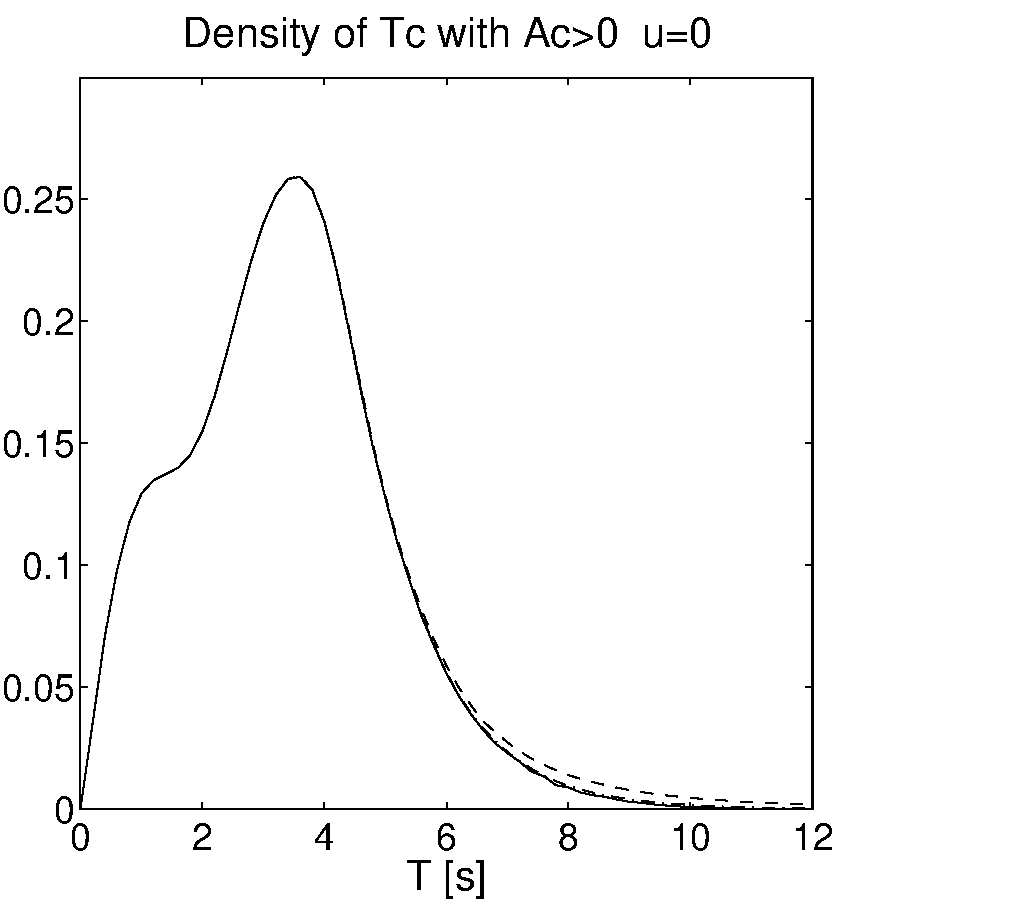
\includegraphics[width=\defwidth]{fig41a_2017}
\end{minipage}}%
\hfill
\subfigure[]{%
\begin{minipage}[b]{0.49\textwidth}%
\label{fig71b}
\centering 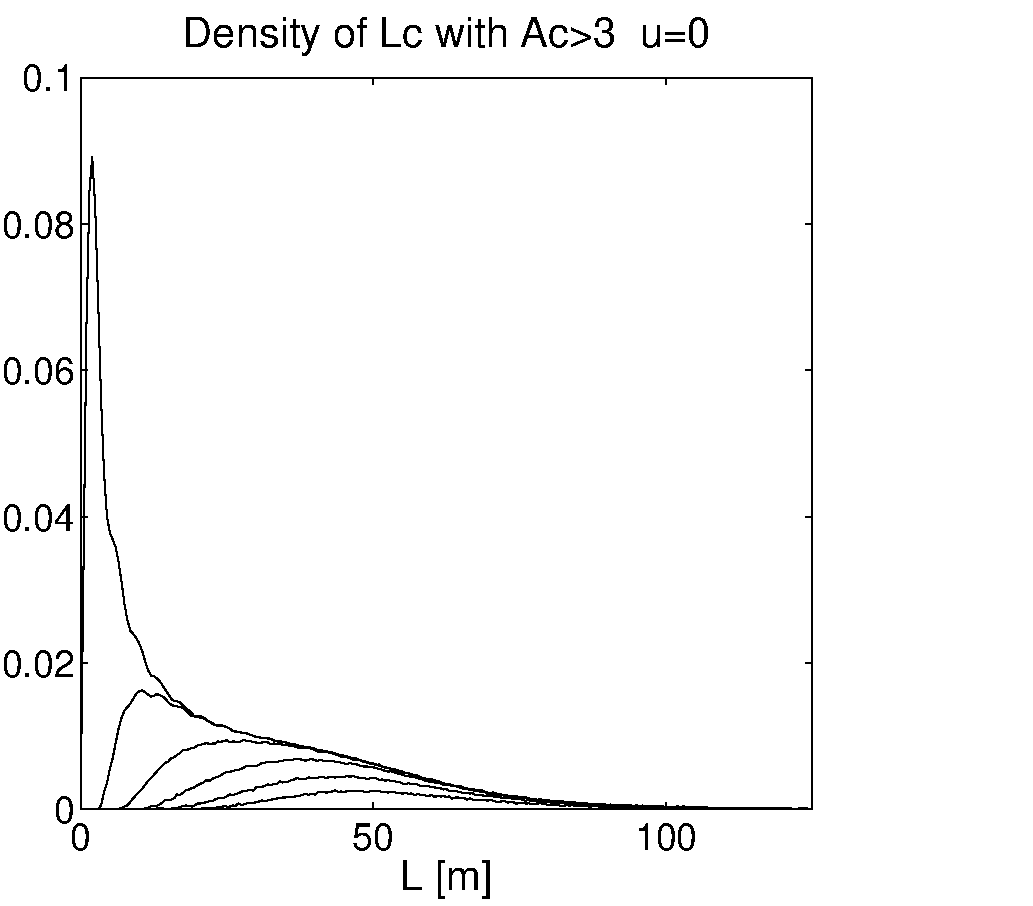
\includegraphics[width=\defwidth]{fig41b_2017}
\end{minipage}}
\vspace{-3mm}
  \caption[Density of crest period {\tt Tc} and  crest length
  {\tt Lc}]{
(a) Densities {\tt f\_tc\_1} (solid), {\tt f\_tc\_2} (dashed),
and {\tt f\_tc\_4} (dash dotted)
of crest period {\tt Tc} for Torsethaugen spectrum {\tt ST}.
(b) Densities of crest length
{\tt Lc}, (most peaked curve) compared to the density when restricted
to waves with crest height {\tt Ac} more than 10\%, 20\%, 30\%, 40\%, 50\%
of the significant wave height above the still water level,
for Gaussian sea with the Torsethaugen spectrum with {\tt Hs = 6[m]}.
Lowest curve corresponds to {\tt Ac > 3[m]}; the exact proportion is 10.2\%, 
according to Table~\ref{tab:AcCDF}.
}
  \label{fig71}
\end{figure}


The last argument in the calls above to {\tt spec2tpdf} is worth
special attention, and we will later study its effect in detail.
It controls the numerical algorithm that computes the density. Here, we
only note that a positive choice, here {\tt 4}, gives an upper bound
to the density, more accurate and more time consuming the higher the value,
while a negative value, here {\tt -1}, given an almost unbiased value in much shorter time.
\end{cex}

\subsubsection{Crest length}
\begin{cex}{Ex_Torseth}  {\sl (Crest length)} \label{pageTorsethCrestLength}
We then turn to the density of crest length for the Torsethaugen spectrum.
It can be computed using the same function {\tt spec2tpdf}, we just
change the input {\tt def} variable {\tt 'Tc'} to {\tt 'Lc'}.
{\small\begin{verbatim}
      f_Lc = spec2tpdf(ST,[],'Lc',[0 100 151],[],-1);
      pdfplot(f_Lc,'-.'), hold on
\end{verbatim}}

The crest length density has a sharp peak for very short waves
-- the wave-number spectrum is much  more broad banded than
the frequency spectrum; see \cite{LindgrenEtal1998Relation}
for a general comparison of wave period and wave length.
However, the short waves have small crests and
should be considered as 'noise' rather than as apparent waves.
Consequently, we may wish to compute the proportion of waves that have crest
higher than a certain proportion of the significant wave height, e.g.\
25\%, i.e.\ one standard deviation, \verb+Hs/4 = 1.5[m]+,
and give the density of the crest length for these waves. This can be
done by specifying an extra argument {\tt h = 1.5} in the call to \verb+spec2tpdf+.
{\small\begin{verbatim}
      f_Lc_1 = spec2tpdf(ST,[],'Lc',[0 100 151],1.5,-1);
      pdfplot(f_Lc_1)
\end{verbatim}}

Figure~\ref{fig71}(b) presents the results when the crest height is
restricted to more than 10\%, 20\%, 30\%, 40\%, 50\% of the
significant wave height. and we can see that all short
waves in fact were small. (The algorithm produces some
very small negative density values. These have been removed before
the plotting; see the following section on numerical accuracy,
Section~\ref{subsec:numerical accuracy}.)

The proportion of waves with
crests above 1.5~[m] (one standard deviation) is computed by the following commands.
{\small\begin{verbatim}
      simpson(f_Lc.x{1},f_Lc.f)
      simpson(f_Lc_1.x{1},f_Lc_1.f)
\end{verbatim}}
\noindent Taking the ratio, we can see that
more than half of the waves are small,
about 37\% of the waves have crests above 1.5~[m]. Similar calculations
for the curves in Figure~\ref{fig71}(b), give the proportions of crests
above the levels in Table~\ref{tab:AcCDF}.\index[xcmds]{{\tt spec2Acdf}}
\index[xcmds]{{\tt spec2tpdf}}
\end{cex}

\begin{table}[t]
\centerline{
\begin{tabular}{l|cccccc}
level [m] & 0.6 & 1.2 & 1.5 & 1.8 & 2.4 & 3.0 \\ \hline
proportion of crests above level & 0.607 & 0.435 & 0.367 & 0.305 & 0.191 & 0.102 \\
CDF of crest height {\tt Ac} & 0.391 & 0.563 & 0.630 & 0.693 & 0.806 & 0.895
\end{tabular}}
\caption[Crest height distribution]{Second row:
proportion of crest heights above a level, computed by {\tt spec2tpdf};
Third row: CDF of crest height computed by {\tt spec2Acdf}.}
\label{tab:AcCDF}
\end{table}

\subsubsection{Crest height}
From a statistical viewpoint the crest period distribution is uniquely defined as 
the empirical distribution of the time between  mean level upcrossings and 
the following downcrossing. It is linked to a fixed observation point and 
an ``infinite'' observation interval. Similarly, crest length distribution is 
the empirical distribution of the distance between mean level up- and downcrossings. 
It is linked to a fixed time and a fixed, ``infinitely long'', observation transect 
on the ocean surface. 
Discussing crest height distribution, the maximum height between an up- and a 
downcrossing, we obviously have to decide which observation scheme is used. 
Fortunately, the \progname{} routine {\tt spec2Acdf} handles both alternatives, 
depending on the type of spectrum we use.. 

\begin{cex}{Ex_Torseth} {\sl (Crest height)}\label{pageTorsethCrestHeight}
The table of the proportion of high crest waves is related
to the cumulative distribution function (cdf) of the crest height {\tt Ac}
in a natural way. The routine {\tt spec2Acdf} computes and plots
the cdf directly, both for the crest height over a crest period in time
and for the crest height over a crest length in space. It also plots the Rayleigh approximation. 

The following commands creates empirical and theoretical crest height distributions 
in time and in space for Gaussian waves with Torsethaugen frequency spectrum. 
The vector {\tt T} contains 100 replicates of 400 seconds of time wave simulation, the vector 
{\tt L} contains 100 replicates of 4000 meters of space wave simulation. {\tt AcT, AcL} 
are the time and space observed crest heights, respectively.  
{\small\begin{verbatim}
      clf; Hs = 6;
      r = (0:0.12:1.1*Hs)';
      F_Ac_s1_T = spec2Acdf(ST,[],'Tc',[0 12 61],r,-1); hold on
      T = spec2sdat(ST,[40000,100],0.01);
      [SteepT,HeightT,AcT] = dat2steep(T);
      plotedf(AcT,'-.')
      F_Ac_s1_L = spec2Acdf(ST,[],'Lc',[0 125 251],r,-1);
      L = spec2sdat(spec2spec(ST,'k1d'),[40000 100],0.1);
      [SteepL,HeightL,AcL] = dat2steep(L);
      plotedf(AcL,'-.')
      plot(r,1-exp(-8*r.^2/Hs^2)), hold off
\end{verbatim}}

Figure~\ref{fig:AcCDF}
shows the empirical distribution of {\tt Ac} in a long simulation in time,
and the theoretical distribution functions for crest height
in time and in space computed by {\tt spec2Acdf}, as well as the Rayleigh approximation from
Section~\ref{ss:Rayleighapproximation}. The simulations contain {\tt 9255}
space wave crests and {\tt 5823} time wave crests. The agreement between the
empirical and theoretical distribution functions is very good. 
The Rayleigh distribution gives a good approximation of the time crest height 
for large crest values but over-estimates the smallest crests. \index[xcmds]{{\tt dat2steep}}
\index[xcmds]{{\tt spec2Acdf}}\index[xcmds]{{\tt spec2spec}}
\index[xcmds]{{\tt spec2sdat}}
It does not work 
for space waves.

The third row in Table~\ref{tab:AcCDF}
shows the cdf values for crest height in space computed by {\tt spec2Acdf}.
The sum of the second and third row should be one; here, 
all sums in the table are greater than {\tt 0.997}.
\end{cex}

\begin{figure}[tbh]
\centerline{
%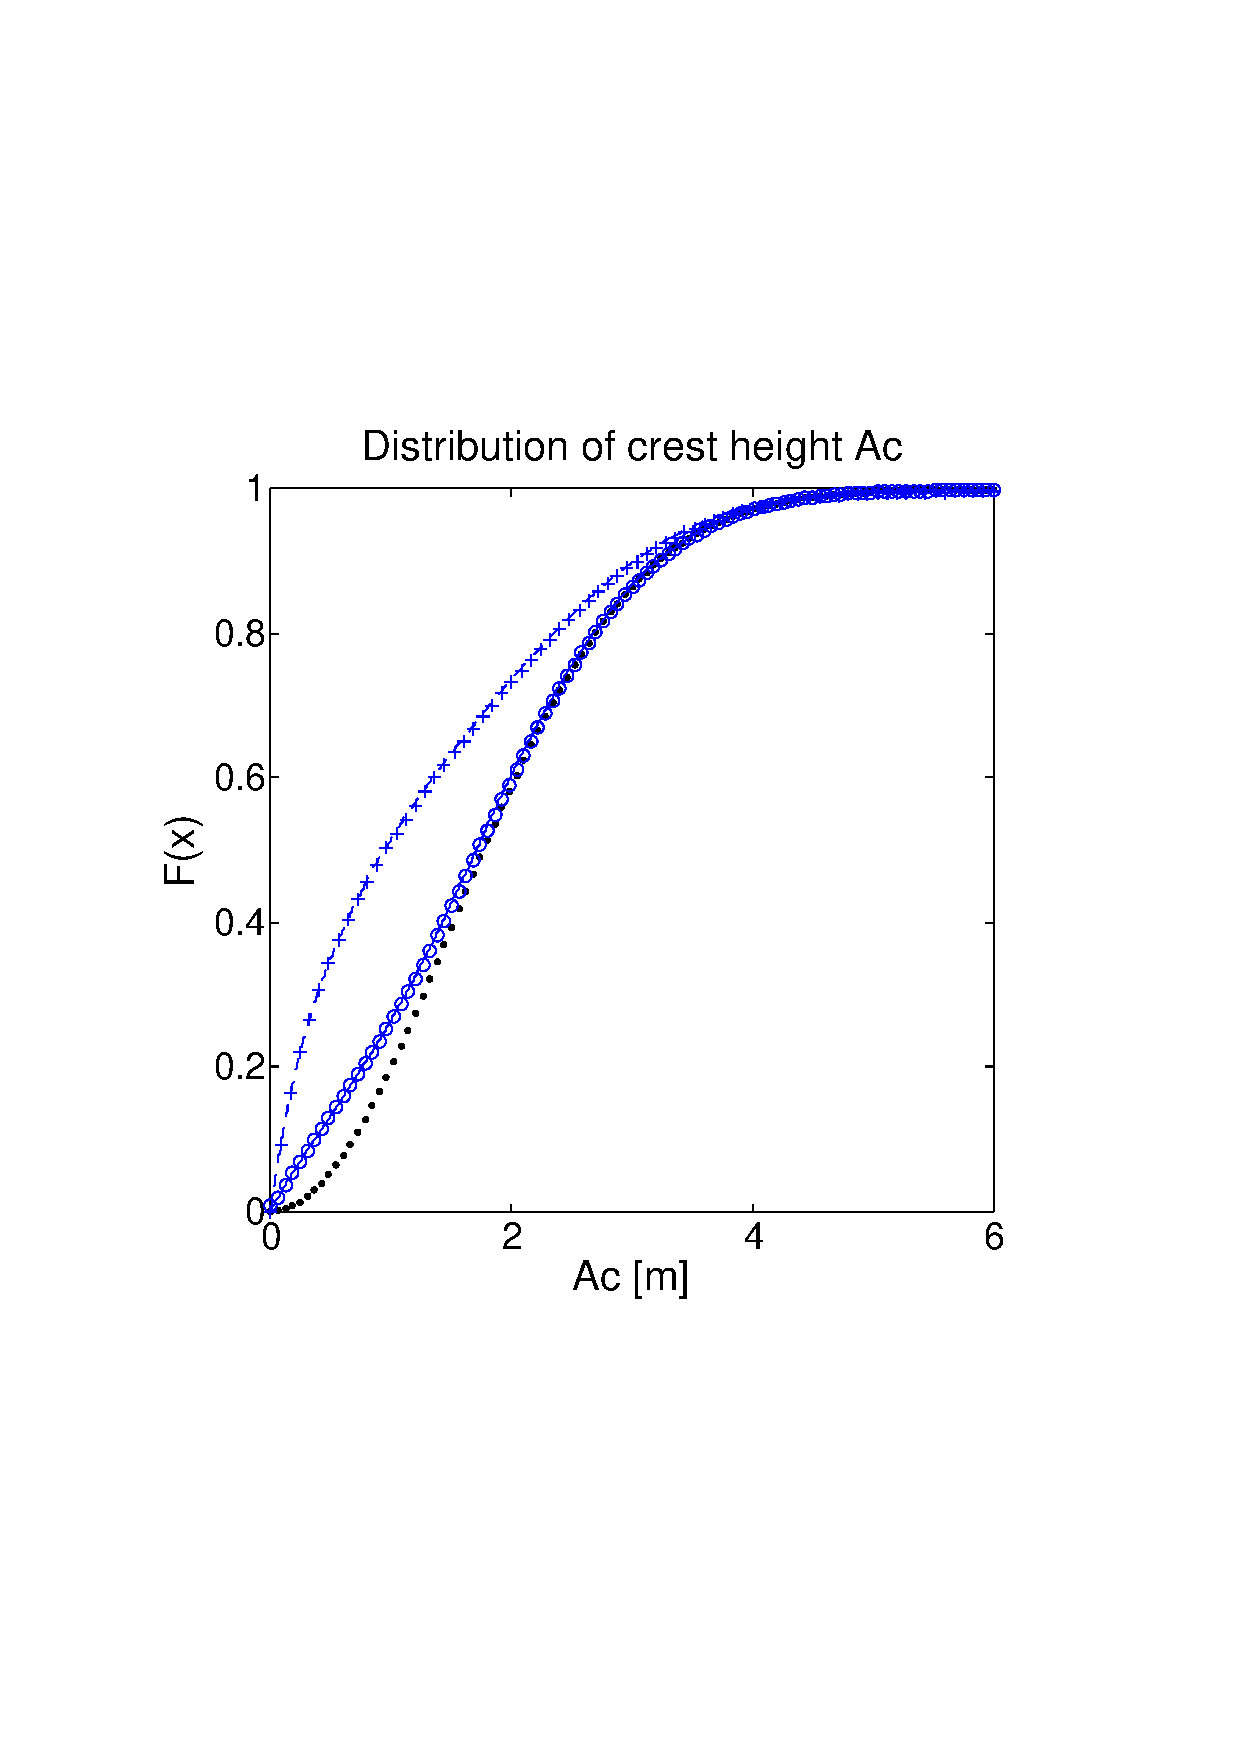
\includegraphics[height=60mm]{figAcCDF}
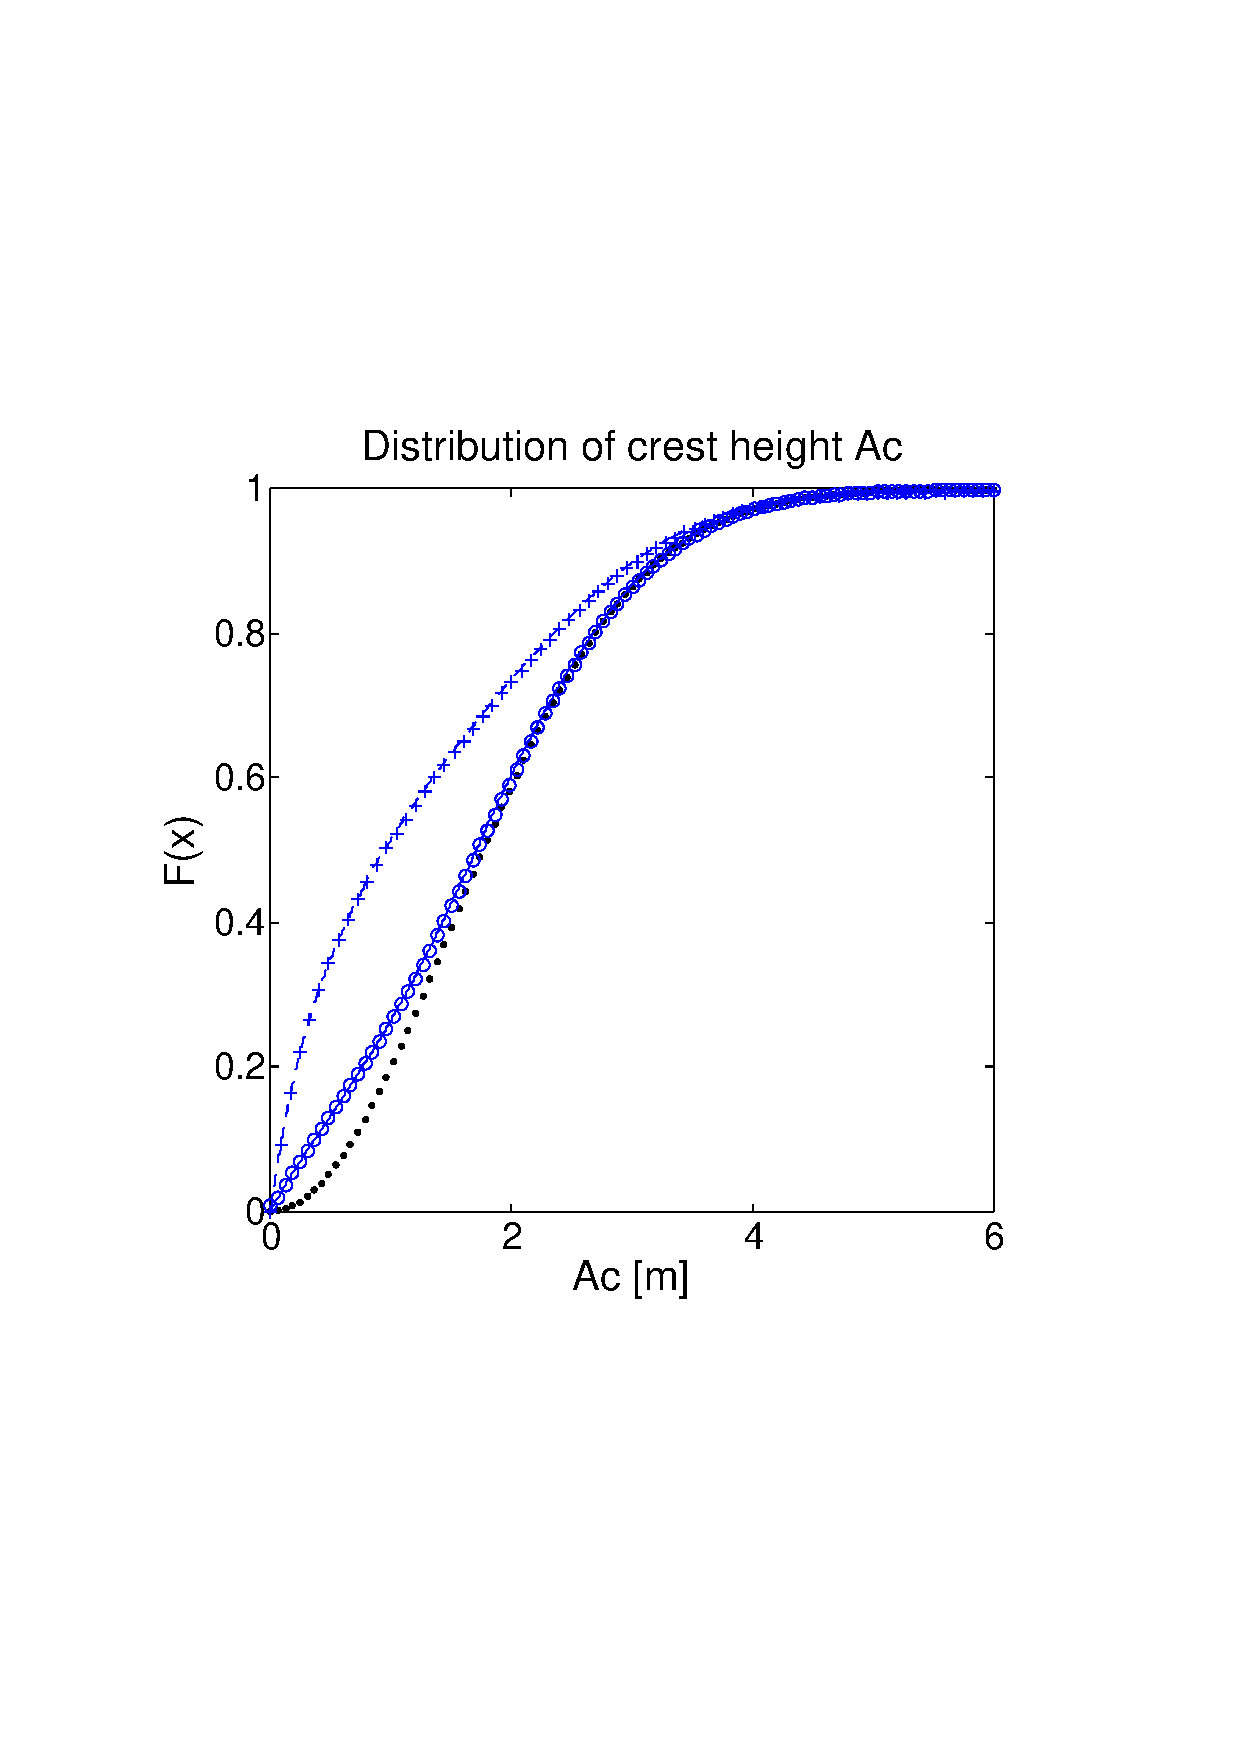
\includegraphics[width=\onefigwidth]{figAcCDF}
%\hspace{5mm}
%\includegraphics[height=60mm]{fig42}
}
\vspace{-3mm}
\caption[Cumulative distribution for crest height Ac]%
{Cumulative distribution (cdf) for crest height {\tt Ac}
with Torsethaugen spectrum {\tt ST}.
Curves most to the left = theoretical (solid)  and empirical
(dash dotted) cdf for {\tt Ac} over a crest length. 
Middle curves show theoretical and empirical
cdf for {\tt Ac} over a crest period. Curve most to the right 
is the cdf for the Rayleigh approximation.}
\label{fig:AcCDF}
\end{figure}

\begin{figure}[tbh]
\centerline{
\includegraphics[height=60mm]{fig42a_2017}
\hspace{5mm}
\includegraphics[height=60mm]{fig42_2017}
}
\vspace{-3mm}
\caption[Density and cumulative distribution for
{\tt Lc} with directional spreading]%
{Computed pdf (left) and cdf (right)
for {\tt Lc} in Gaussian sea with Torsethaugen
spectrum with different spreading: unidirectional spectrum {\tt S1}
(solid line) ; frequency independent spreading {\tt SD1}
(dash-dotted line); frequency dependent spreading {\tt SD12}
(dashed line).}
\label{fig:42}
\end{figure}

\begin{cex}{Ex_Torseth}{\sl (Directional spreading)} 
We finish this example by considering the Torsethaugen spectrum
with the two different spreading functions {\tt STD1} and {\tt STD12}.
In Figures~\ref{fig:00sima} and \ref{fig:00simb} we presented simulations of the sea surfaces
with these spectra. From the figures we expect that the two crest length
distributions should be different.
(Obviously, the crest period densities are identical).
In the directional sea we have to define the azimuth of the
line for which the crest length should be computed (the default value
is zero). Now, the directional spectra {\tt STD1} and {\tt STD12}
have different main wave directions, $90^o$ and $0^o$ degrees, respectively,
and hence we shall choose different azimuths for the two spectra.
More precisely, for both cases we shall consider heading waves; this
is achieved using the function {\tt spec2spec}.
{\small\begin{verbatim}
      f_Lc_d1 = spec2tpdf(spec2spec(STD1,'rotdir',pi/2),[],...
                'Lc',[0 200 201],[],-1);
      pdfplot(f_Lc_d1,'-.'), hold on
      f_Lc_d12 = spec2tpdf(STD12,[],'Lc',[0 200 201],[],-1);
      pdfplot(f_Lc_d12), hold off

      figure(2)
      dx = f_Lc.x{1}(2)-f_Lc.x{1}(1);
      dx1 = f_Lc_d1.x{1}(2)-f_Lc_d1.x{1}(1);
      dx12 = f_Lc_d12.x{1}(2)-f_Lc_d12.x{1}(1);
      plot(f_Lc.x{1},cumsum(f_Lc.f)*dx), hold on
      plot(f_Lc_d1.x{1},cumsum(f_Lc_d1.f)*dx1,'-.')
      plot(f_Lc_d12.x{1},cumsum(f_Lc_d12.f)*dx12,'--'), hold off
\end{verbatim}}

As expected, after examination of the simulated sea surfaces in
Figures~\ref{fig:00sima} and \ref{fig:00simb}, the crest length
for the two directional spectra are different.
The sea with frequency dependent spreading seems to be more irregular.
We can see in Figure~\ref{fig:42} that waves with frequency
independent spreading are only slightly
longer than the waves in unidirectional sea, while the
crest length of both seas are much shorter than for frequency
dependent spreading. 
%From Figure~\ref{fig:directspect} it is clear
%that the spectrum with frequency independent spreading function is more
%similar to the unidirectional spectrum than that with the
%frequency dependent spreading.
\end{cex}

\subsection{Numerical accuracy and computational speed}
\label{subsec:numerical accuracy}
\index[xentr]{numerical accuracy}
The basic algorithm in the routine {\tt spec2tpdf} computes a
finite-dimensional approximation to an "infinite-dimensional"
normal expectation. The last input in all the previous calls
to the routine is a parameter called {\tt nit}, and it
determines both the integration method and the dimensionality
of the computed integral.
Important references on how to compute normal probabilities are
\cite{AmbartzumianEtal1998Multinormal,Brodtkorb2004Probability,
Brodtkorb2006Evaluating,Genz1992Numerical,GenzAndKwong2000Numerical,
Rychlik1992Confidence}.

The {\tt nit} parameter can be positive, negative, and zero.
Positive {\tt nit} values use numerical, deterministic, integration
algorithms, while negative values use a simulation technique
based on importance sampling; see \cite{Brodtkorb2004Probability,
Brodtkorb2006Evaluating} for a review of different methods.

The methods with positive {\tt nit} are very reliable and have
been tested on different wave problems since the first version was
used already in 1987; see \cite{Rychlik1987Regression}. As default,
they give an upper bound to the densities.
The integration methods corresponding to negative {\tt  nit} values are
%still under tests and modifications. However, they are 
often much faster and also very accurate in cases when the
deterministic method has troubles with too long execution times;
see \cite{Lindgren2017} for examples. 

Although the method  with negative {\tt nit} is based on
simulation, the accuracy is still controlled. If the number of
simulations is too small to achieve the required accuracy
the program gives an error statement with an estimate of
the possible error in the computed density.

One should be aware that both positive and negative {\tt nit} values
can produce negative density values with {\tt spec2tpdf}. This is
the result of the way  the densities are computed, namely as differences
between "cumulative distribution type" functions. Then, small numerical
variations may cause negative density estimates, mostly for very
small density values.

The routine {\tt spec2tpdf} is the \ML{} interface to a
{\sc Fortran} program. All programs computing exact
densities of different wave characteristics
can be reformulated in such a way that the density is written as a
certain multidimensional integral of a function of Gaussian
variables; see \cite{LindgrenAndRychlik1991Slepian} for more details.
This integral is computed using a {\sc Fortran} module called
{\tt RIND}. There is also a \ML{} interface called
{\tt rind}\index[xcmds]{{\tt rind}} which can be
used to test programs for new wave characteristics.

An example is a function {\tt spec2tpdf2} which uses the program
{\tt rind}. The program is slower than {\tt spec2tpdf},
and it does not have an option that allows to choose waves with crest
above some level, but on the other hand it is easier to use for
experimentation, and it can also be used to learn how to
create own programs.

Besides the parameter {\tt nit}, the input parameter {\tt speed} will
also control the accuracy of the computations in module {\tt trgauss};
see the help text to the routines for information.

\begin{remark}
The accuracy of the numerical computations depends on the parameters {\tt nit} and {\tt speed} in 
a natural and predictable way. Of course, also the choise of  grid size affects the 
accuracy; some of the algorithms are very sensitive to short time or space steps and can 
produce covariance matrices which are not positive definite. 

\ML{} version, computer CPU, and RAM memory size, all affect speed. More subtle effects of hardware implementation 
can affect some computed small probabilities, of interest in applications. In the examples we 
present many numerical results and execution times, and the reader is advised to make own experiments 
to become familiar with these characteristics.  
\end{remark}

\begin{cex}{Ex_Torseth} {\sl (Numerical accuracy and the parameter {\tt nit})} 
We shall exemplify the use of the parameter {\tt nit} by computing the
crest length density for the directional spectrum with frequency
independent spreading.
We shall also use the slower program {\tt spec2tpdf2} for
illustration. We fix the speed and method by setting an option variable.\index[xcmds]{{\tt spec2tpdf2}}
{\small\begin{verbatim}
      opt1 = rindoptset('speed',5,'method',3);
      STD1r = rotspec(STD1,pi/2);
      f_Lc_d1_5 = spec2tpdf(STD1r,[],'Lc',[0 200 201],[],5);
      f_Lc_d1_3 = spec2tpdf(STD1r,[],'Lc',[0 200 201],[],3);
      f_Lc_d1_2 = spec2tpdf(STD1r,[],'Lc',[0 200 201],[],2);
      f_Lc_d1_0 = spec2tpdf(STD1r,[],'Lc',[0 200 201],[],0);
      f_Lc_d1_neg = spec2tpdf(STD1r,[],'Lc',[0 200 201],[],-1);
      f_Lc_d1_n4 = spec2tpdf2(STD1r,[],'Lc',[0 200 201],opt1);

      pdfplot(f_Lc_d1_5), hold on
      pdfplot(f_Lc_d1_2), pdfplot(f_Lc_d1_3)
      pdfplot(f_Lc_d1_0), pdfplot(f_Lc_d1_neg)
      pdfplot(f_Lc_d1_n4,'LineWidth',2,'-.')
      simpson(f_Lc_d1_n4.x{1},f_Lc_d1_n4.f)
\end{verbatim}}
\index[xcmds]{{\tt rotspec}}

\begin{figure}[tbh]
\subfigure[]{%
\begin{minipage}[b]{0.5\textwidth}%
\centering \includegraphics[height=60mm]{fig43a_2017}
\end{minipage}}%
\hfill
\subfigure[]{%
\begin{minipage}[b]{0.5\textwidth}%
\centering \includegraphics[height=60mm]{fig43b_2017}
\end{minipage}}
\vspace{-3mm}
  \caption[Comparison of crest length densities]{
(a) Approximations by different methods and accuracy
of the crest length for the directional
spectrum {\tt STD1r}  with frequency independent spreading.
The top solid curves are computed with
positive {\tt nit = 0 (top), 2, 3, 5}, and negative
{\tt nit = -1 (bottom)}, in routine {\tt spec2tpdf},
while the dash-dotted curve has negative
{\tt nit} with routine {\tt spec2tpdf2}.
(b) Solid curve = the empirical density of crest
length {\tt Lc} with crest height {\tt Ac > 1.5[m]},
dash-dotted curve is the
normalized computed density {\tt f\_Lc\_1}.
}
\label{fig72}
\end{figure}

The execution times for the densities were 150 seconds, 5.6 seconds, 1.3 seconds,
0.13 seconds, 2.4 seconds, and 3.7 seconds, respectively.
In Figure~\ref{fig72}(a) the different approximations are presented
and we can see how the density decreases with increasing positive {\tt nit}.
The negative {\tt nit} involves some random number integration methods,
but we can hardly see that the computed density is actually a random
function. Most problems are less numerical demanding and {\tt nit=2}
often suffices, but here clearly the negative {\tt nit} is preferable.

In Figure~\ref{fig72}(b) we compare an empirical density of crest length
{\tt Lc}, conditioned on crest height {\tt Ac > 1.5[m]}, based on 
 500~000 observed waves, with the normalized
density {\tt f\_Lc\_1} from page~\pageref{fig71}, computed with
{\tt nit = -1}. The agreement is almost perfect.
\end{cex}
\index[xentr]{wave distributions!computation of densities!
crest length and period|)}
\index[xentr]{crest!period|)}
\index[xentr]{crest!length|)}

\subsection{Wave period and wave length}

\index[xentr]{wave distributions!computation of densities!
wave length and period|(}
\index[xentr]{wave!period|(}
\index[xentr]{wave!length|(}
In the previous sections we described routines for the marginal
distributions of crest and trough periods, and height, {\tt Tc},
{\tt Tt}, {\tt Ac},  and
the corresponding crest and trough lengths, {\tt Lc}, {\tt Lt}.
We also showed how to limit the population to waves for which
the crest (trough) amplitudes are above some predetermined threshold.

We now turn to the wave period,  {\tt Tu = Tc+Tt}, which is the time
between two successive upcrossings of the still water level {\tt u}.
It is related to, but not equal to,
the crest-to-crest wave period {\tt Tcc}, which is
the time span between two successive crests. The density of {\tt Tu}
can be computed using the function
{\tt spec2tccpdf}\index[xcmds]{{\tt spec2tccpdf}}.
The wave length {\tt Lu} or encountered wave period
can also be computed by {\tt spec2tccpdf},
with just a few inputs to be modified; see the help text.
Hence, these variables shall not be discussed here any more.

The computations using {\tt spec2tccpdf} are slower than those using
{\tt spec2tpdf}, since  one needs to compute the joint density of
{\tt Tc} and {\tt Tt} and then integrate the
convolution to get {\tt Tu = Tc+Tt}. 
It should be mentioned that, in addition to the methods to reduce
computation time, one of the best methods to speed up computation is to
cut off high frequencies in the spectrum.
The syntax of {\tt spec2tccpdf} is almost identical to that of
{\tt spec2tpdf}, and hence we limit ourselves to a few examples.

\begin{rtex}{Ex_Seadatawavedistributions}{Sea data wave distributions}
In order to make comparisons with the wave characteristic
distributions in  {\tt sea.dat} we shall use the estimated spectrum \verb+SS+, see
Example~\ref{Ex_sea_statistics} on pages \pageref{Ex_sea_statistics}
and \pageref{fig2_spc}.
We first re-compute the spectrum estimate and the transformation to
Gaussianness, and extract some characteristics.

{\small\begin{verbatim}
      xx = load('sea.dat');
      x = xx;
      x(:,2) = detrend(x(:,2));
      SS = dat2spec(x);
      si = sqrt(spec2mom(SS,1));
      SS.tr = dat2tr(x);
      Hs = 4*si
\end{verbatim}}
\noindent The estimated spectrum is plotted in Figure~\ref{fig:seaspectrum},
together with pointwise 95\% confidence intervals. 

Note that the spectrum contains a transformation 
field {\tt SS.tr}, and recall the {\sc Important note 1} on page~\pageref{ImpNote_1}. 
If you want to simulate new versions of {\tt sea.dat} by {\tt spec2sdat} you must 
normalise the spectrum to have $m_0 = 1$.
\end{rtex}

\begin{figure}[tbh]
\centerline{
\includegraphics[width=\narrowfigwidth]{seaspectrum}
}
\vspace{-3mm}
\caption[Estimated sea spectrum]{Estimated spectrum {\tt SS} for data
{\tt sea.dat} with confidence bands.}
\label{fig:seaspectrum}
\end{figure}

\begin{cex}{Ex_Seadatawavedistributions}{\sl (Crest period)} 
We first consider the crest period,
as we did in Example~\ref{Ex_Torseth} 
on page \pageref{pageTorsethCrestPeriod}, and also the proportion of
crests with \label{page:Ex7a}
significant crest height, i.e.\ {\tt Tc} when {\tt Ac > Hs/2}, in the same way as we did for crest length.
 %in Example~\ref{Ex_Torseth} 
%on page~\pageref{pageTorsethCrestLength}. 
After that we
will do the same for wave period and consider {\tt Tu} when {\tt Ac > Hs/2}.
The proportion of crest periods with significant crest height should be the
same as the proportion of wave periods with significant crest height,
i.e.\ {\tt Tu} when {\tt Ac > Hs/2}. 
The difference between the two proportions gives an indication of 
the accuracy in the computation of the convolution {\tt Tu = Tc + Tt}.

We can also compare the calculated proportion of significant crests
with the proportion observed in data and with the approximative
Rayleigh model. Finally, we estimate the density using KDE from data
and compare to the theoretically computed one, based on the transformed
Gaussian model. \index[xcmds]{{\tt kde}}

For completeness we again estimate the transformation and find wave
characteristics in the signal. The crest period, {\tt Tc}, distribution,
estimated from data, and the computed density are almost identical,
except for very short waves; see Figure~\ref{fig73}(a), obtained by
the following commands. Note the last output variable 
{\tt yn} in the call to {\tt dat2steep}, which
is an interpolated series, to be used later, when we need more exact values 
for the wave periods.\label{Interpol_yn}
{\small\begin{verbatim}
      method = 0; rate = 2;
      [S,H,Ac,At,Tcf,Tcb,z_ind,yn] = dat2steep(x,rate,method);
      Tc = Tcf+Tcb;
      t = linspace(0.01,8,200);
      f_tc1emp = kde(Tc,{'L2',0},t);
      pdfplot(f_tc1emp), hold on
      f_tc1 = spec2tpdf(SS,[],'Tc',[0 8 81],0,4);
      Chk1 = simpson(f_tc1.x{1},f_tc1.f) %Integral should be one
      pdfplot(f_tc1,'-.'), hold off
\end{verbatim}}

We next compute the density of crest period,
but now for waves with significant crest height, i.e.\ waves for
which {\tt Ac > Hs/2}. In the following call to
{\tt spec2tpdf} the restriction to {\tt Ac > Hs/2} is
indicated by the argument~\verb+[Hs/2]+.
{\small\begin{verbatim}
      nit = 4;
      f_tc2 = spec2tpdf(SS,[],'Tc',[0 8 81],[Hs/2],nit);
      Pemp = sum(Ac>Hs/2)/sum(Ac>0) 
      			  %Observed proportion of high crests
      Chk2 = simpson(f_tc2.x{1},f_tc2.f) 
      			  %Integral should be equal to probability of high crests
      index = find(Ac>Hs/2);
      f_tc2emp = kde(Tc(index),{'L2',0},t);
      f_tc2emp.f = Pemp*f_tc2emp.f;
      pdfplot(f_tc2emp), hold on
      pdfplot(f_tc2,'-.'), hold off
\end{verbatim}}

The observed frequency of significant crests, {\tt Pemp = 0.1778} is 
close to the theoretically computed values, {\tt Chk2 = 0.1802} with {\tt nit = 5} and 
{\tt Chk2 = 0.1816} with {\tt nit = 4},
obtained with computation times of 18~seconds and 4~seconds, respectively. 
A finer grid, {\tt [0 8 161]} instead of {\tt [0 8 81]} in \verb+f_tc2+, will give an 
almost exact agreement with the empirical frequency with four times the computation time. 

Observe that the Rayleigh approximation would give a
probability equal to 0.1353. This is not surprising since crests in
non-Gaussian sea tend to be higher than those in Gaussian sea.

Clearly, by changing the input {\tt Hs/2} to any other fixed level
{\tt h}, and integrating the resulting density we obtain
approximations to the probability {\tt P(Ac > h)}.
When {\tt h} is a vector then it is more efficient to use the program
{\tt spec2Acdf}\index[xcmds]{{\tt spec2Acdf}} to compute {\tt P(Ac > h)},
as in the crest height Example~\ref{Ex_Torseth} 
on page~\pageref{pageTorsethCrestHeight}. 
However, before using the
program it is important to first use {\tt spec2tpdf} and check that the
computed density integrates to one. If not, the inputs {\tt param} and
{\tt nit} have to be changed. Note that the integral {\tt Chk1} is slightly 
greater than one. 

\begin{figure}
\subfigure[]{%
\begin{minipage}[b]{0.5\textwidth}%
%\centering \includegraphics[width=\defwidth]{fig7_tb_2017}
\centering \includegraphics[height=60mm]{fig7_tb_2017}
\end{minipage}}%
\hfill
\subfigure[]{%
\begin{minipage}[b]{0.5\textwidth}%
%\centering \includegraphics[width=\defwidth]{fig7_t2b_2017}
\centering \includegraphics[height=60mm]{fig7_t2b_2017}
\end{minipage}}
\vspace{-3mm}
  \caption[Estimated and theoretical
density of crest periods in {\tt sea.dat}]{
(a) Estimated density (KDE) of crest periods in {\tt sea.dat} (solid line)
compared with theoretically
computed using {\tt spec2tpdf} (dashed line). (b) The same for the
waves with significant crest, i.e.\ {\tt Ac > Hs/2}.
}
\label{fig73}
\end{figure}

Observe that in this section we are analysing apparent waves
in time. If the input {\tt 'Tc'} in {\tt spec2tpdf} is replaced by
{\tt 'Lc'}, then we would consider waves in space and the proportion
of significant crest would probably be very different.
\end{cex}

\begin{cex}{Ex_Seadatawavedistributions}{\sl (Wave period for high-crest waves)}
We turn now to the more difficult problem of wave
period {\tt Tu = Tc+Tt}, and compute the density for 
waves with significant crest height, {\tt Ac > Hs/2} and
with {\tt At > 0}. As mentioned, this differs from crest period 
Example~\ref{Ex_Torseth} on page~\pageref{pageTorsethCrestPeriod} 
in that it involves the
distribution of the sum {\tt Tc + Tt} of two dependent random variables,
with the same marginal distribution. Since the computations need to be
done with high accuracy (the computed density is different for the
unconditional wave period and for the period of waves with crest below a given
threshold),  % see \cite{BIOPR00} for more detailed discussion),
we need to use a high positive {\tt nit} value, so that the total sum
of the density is close to 0.1789, or use a negative {\tt nit}. 
We begin with negative {\tt nit}, which gives faster results
very close to the true density, and then take {\tt nit = 3}.
{\small\begin{verbatim}
      f_tun = spec2tccpdf(SS,[],'t>',[0 12 61],[Hs/2],[0],-1);
      simpson(f_tun.x{1},f_tun.f)
      f_tu3 = spec2tccpdf(SS,[],'t>',[0 12 61],[Hs/2],[0],3,5);
      simpson(f_tu3.x{1},f_tu3.f)
      pdfplot(f_tun), hold on
      pdfplot(f_tu3,'--'), hold off
\end{verbatim}}

\begin{figure}[tbh]
\subfigure[]{%
\begin{minipage}[b]{0.5\textwidth}%
\centering \includegraphics[height=60mm]{fig7_tcc2b_2017}
\end{minipage}}%
\hfill
\subfigure[]{%
\begin{minipage}[b]{0.5\textwidth}%
\centering \includegraphics[height=60mm]{fig7_tcc22_4b_2017}
\end{minipage}}
\vspace{-3mm}
  \caption[Densities of period {\tt Tu}]{
(a) Densities of upcrossing period {\tt Tu} for waves with significant crest in
the transformed Gaussian  model
for {\tt sea.dat} computed with different degree of
accuracy; (solid line)  {\tt nit=-1}; the dashed line is
computed with {\tt nit=5} and the dash dotted line with {\tt nit=3}.
(b) Densities of period {\tt Tu} for waves with significant crest and
trough in the same model; solid wiggled line {\tt nit=-1}; solid smooth line
 {\tt nit=4}; the dash dotted line is estimated from
 the data with KDE.
}
 \label{fig74}
\end{figure}
The integral of the density \verb+f_tcn+ is 0.1778,
which is close to the previously computed value 0.1789.
However, the execution time was 66 seconds, compared to
21~seconds for \verb+f_t2+. The choice {\tt nit=3} takes 3~minutes
and give the integral 0.15. We have checked the program with
{\tt nit=5} (execution times 66~minutes), and the integrals was 0.17.
The densities are shown in Figure~\ref{fig74}(a). We can see that
the density computed using {\tt nit=-1} (dash-dotted line) is quite
accurate, even if it slightly
wiggly, being a random function with very small variance, and errors
compensate each other giving almost perfect total probability mass.
Note that another call of the program would give slightly different
values and the total mass would also be changed.
\end{cex}

\begin{cex}{Ex_Seadatawavedistributions}{\sl (Wave period for high-crest, deep-trough waves)}
We finish the example with an even more
interesting case, the density of wave period of waves with both
significant crest and significant trough, i.e.\ really big waves.
We  first estimate the probability of such waves in the data; then we
use the interpolated series {\tt yn} from page~\pageref{Interpol_yn}.
{\small\begin{verbatim}
      [TC tc_ind v_ind] = dat2tc(yn,[],'dw');
      N = length(tc_ind);
      t_ind = tc_ind(1:2:N);
      c_ind = tc_ind(2:2:N);
      Pemp = sum(yn(t_ind,2)<-Hs/2 && ...
             yn(c_ind,2)>Hs/2)/length(t_ind)
      ind = find(yn(t_ind,2)<-Hs/2 && yn(c_ind,2)>Hs/2);
      spwaveplot(yn,ind(2:4))
      Tu = yn(v_ind(1+2*ind),1)-yn(v_ind(1+2*(ind-1)),1);
      t = linspace(0.01,14,200);
      f_tu2_emp = kde(Tcc,{'L2',0},t);
      f_tu2_emp.f = Pemp*f_tu2_emp.f;
      pdfplot(f_tu2_emp,'-.')
\end{verbatim}}
\index[xcmds]{{\tt spwaveplot}}

The probability is estimated to be
\verb+Pemp = 0.0370+, which is slightly higher
than what we could expect if high crests and low troughs occur
independently of each other (the probability would then be less than 0.025).

We turn now to computation of the probability using {\tt spec2tccpdf}
with {\tt nit=-1}. However, we are here in a situation when the
error in computations is of the order $10^{-3}$, which is comparable
to the values of the density itself. Hence the computed function
will look very noisy.
{\small\begin{verbatim}
      f_tu2_n = spec2tccpdf(SS,[],'t>',[0 12 61],[Hs/2],[Hs/2],-1);
      simpson(f_tu2_n.x{1},f_tu2_n.f), hold on
      pdfplot(f_tu2_n), hold off
\end{verbatim}}

The execution time is less than one minute, and the
computed probability with \verb+nit = -1+ is 0.0358,
which is well in agreement with the number estimated from data. 
The more time-demanding \verb+nit = 4+ gives a much smoother 
pdf curve with almost the same integral, with an execution time of 15~minutes.

\index[xentr]{wave distributions!computation of densities!
wave length and period|)}
\index[xentr]{wave!period|)}
\index[xentr]{wave!length|)}

In Figure~\ref{fig74}(b) we see the computed densities of wave
period for these big waves. Those are well concentrated around the
mean value. It is also compared to the KDE estimator. We have not tried to
tune up the estimator that is based on only 20 values and hardly can
be considered as accurate.\end{cex}

\section{Joint density of crest period and crest
  height}\label{sec:joint_crest_period_and_height}
\index[xentr]{wave distributions!computation of densities!
joint crest height/period|(}

In this section we shall present programs for joint characteristics
of apparent waves. We shall be mostly concerned with crest period,
crest position, and crest height. Since we also want to compare the
theoretically derived densities with observations we wish to study
a longer record of measurements than we did in the previous section.
By doing so we will have more reliable statistical estimates of
the densities, but on the other hand we face the problem that the
sea state can change during the measured period -- the process is
simply not stationary.

The data come from the Gullfaks C platform, see
Figure~\ref{fig7northsea}(a). See the help text of {\tt gfaksr89}
for a detailed description of the data  and {\tt northsea}
for the instructions how the map showing location of
the platform was drawn. \index[xcmds]{{\tt gfaksr89}}
\index[xcmds]{{\tt northsea}}\index[xentr]{Gullfaks C platform}

\begin{figure}[htbp]
\subfigure[]{%
\begin{minipage}[b]{0.45\textwidth}%
\centering \includegraphics[height=60mm]{fig7northsea}
\end{minipage}}%
\hfill
\subfigure[]{%
\begin{minipage}[b]{0.55\textwidth}%
\centering \includegraphics[height=60mm]{fig7northsea_s}
\end{minipage}}
\vspace{-3mm}
  \caption[Location of Gullfaks C platform and estimated spectrum]
{Location of Gullfaks C platform (a). The estimated spectrum (b).
}
 \label{fig7northsea}
\end{figure}

\bigskip
\noindent
{\bf WARNING:} In the following examples we run the programs with
maximum accuracy and hence we have long execution times.
Usually one should use simpler and faster approximations at first
experiments with complicated distributions. When one is satisfied with the
results, one should compute the densities
with the desired high accuracy. For testing own problems  we recommend
to start execution of programs with input parameter {\tt speed = 9,8}
(maximal speed is {\tt 9}, the default is {\tt 4}) and {\tt nit = -1, 1},
(default is {\tt 2}).
These choices will produce fast but still useful approximations.

\subsection{Preliminary analysis of data}
\begin{rtex}{Ex_preliminary_analysis}{Analysis of Gullfaks data}
  We begin with loading the data, estimating spectrum, finding the
  transformation {\tt g}, and checking crest period density. Observe that
  the data is sampled with 2.5~[Hz], what may cause some interpolation
  errors in the estimated densities.
{\small
\begin{verbatim}
      yy = load('gfaksr89.dat');
      SG = dat2spec(yy);
      si = sqrt(spec2mom(SG,1));
      SG.tr = dat2tr(yy);
      Hs = 4*si
      v = gaus2dat([0 0],SG.tr); v = v(2)
\end{verbatim}
} \index[xcmds]{{\tt gaus2dat}}
\noindent
The spectrum has two peaks, see  Figure~\ref{fig7northsea}(b).
We are not checking different options to estimate the spectrum,
but use the default parameters.

We shall now extract some simple wave characteristics, {\tt Tc,Tt,Tcf,Ac,At}.
All these are column vectors containing crest period, trough period, position
of crest, crest height, and trough height, respectively.
All vectors are ordered by number of a wave, i.e.\ all vectors contain
characteristic of the {\tt i'th} wave in their position \verb+i+.
{\small
\begin{verbatim}
      [TC tc_ind v_ind] = dat2tc(yy,v,'dw');
      N = length(tc_ind);
      t_ind = tc_ind(1:2:N);
      c_ind = tc_ind(2:2:N);
      v_ind_d = v_ind(1:2:N+1);
      v_ind_u = v_ind(2:2:N+1);
      T_d     = ecross(yy(:,1),yy(:,2),v_ind_d,v);
      T_u     = ecross(yy(:,1),yy(:,2),v_ind_u,v);
      Tc = T_d(2:end)-T_u(1:end);
      Tt = T_u(1:end)-T_d(1:end-1);
      Tcf = yy(c_ind,1)-T_u;
      Ac = yy(c_ind,2)-v;
      At = v-yy(t_ind,2);
\end{verbatim}
} \index[xcmds]{{\tt ecross}}
\noindent
Here we used the routine \verb+ecross+ to interpolate the data to find the exact 
level crossings. 
We then compute the crest period density from spectrum and compare it with
that observed in data.
{\small\begin{verbatim}
      t = linspace(0.01,15,200);
      kopt3 = kdeoptset('hs',0.25,'L2',0);
      ftc1 = kde(Tc,kopt3,t);
      ftt1 = kde(Tt,kopt3,t);
      pdfplot(ftt1,'k'), hold on
      pdfplot(ftc1,'k-.')
      f_tc4 = spec2tpdf(SG,[],'Tc',[0 12 81],0,4,5);
      f_tcn = spec2tpdf(SG,[],'Tc',[0 12 81],0,-1);
      pdfplot(f_tcn,'b'), hold off
\end{verbatim}
} \index[xcmds]{{\tt kde}} \index[xcmds]{{\tt kdeoptset}}

We do not present the graphical result for this computations but simply
comment that the agreement between theory and data is very good for
both densities,
except for observed long waves, which  have somewhat longer periods
(about 0.25 seconds) than theoretically computed.  It is not much for a signal
with 2.5~[Hz] sampling frequency. There is also the possibility that the
swell peak in the spectrum is too much smoothed.
\end{rtex}

\subsection{Joint distribution of crest period and height}
We turn now to the joint density for the wave crest variables
{\tt Tc,Tcf,Ac}. We shall compute the empirical densities
from the observations and compute the theoretical ones from the
transformed Gaussian process with estimated spectrum and the
transformation using the function
{\tt spec2thpdf}\index[xcmds]{{\tt spec2thpdf}}.
This function computes many joint characteristics of the half wave,
i.e.\ the part of the signal between the consecutive crossings
of a still water level -- most of them are simply functions of the
triple {\tt Tc,Tcf,Ac}. (Execute 
{\tt help spec2thpdf} for a complete list).

In a special case, when the so called crest velocity is of interest,
{\tt Vcf=Ac/Tcf}, the joint density of {\tt Vcf,Ac} is computed by
the program {\tt spec2vhpdf}\index[xcmds]{{\tt spec2vhpdf}},
which is a simplified and modified
{\tt spec2thpdf} program.

\begin{cex}{Ex_preliminary_analysis}{\sl (Position and height of  
crest for wave with given period)} 
We shall first consider  waves with
crest period {\tt Tc} $\approx$ 4.5 seconds. Obviously  the position
of the crest of such waves is not constant, but varies from wave to
wave. The following commands estimate the density of crest position
and height for waves with {\tt Tc} $\approx$ 4.5 seconds, and plot the 
results in Figure~\ref{fig76}(a).
{\small\begin{verbatim}
      ind = find(4.4<Tc && Tc<4.6);
      f_AcTcf = kde([Tcf(ind) Ac(ind)],{'L2',[1 .5]});
      plot(Tcf(ind), Ac(ind),'.'), hold on
      pdfplot(f_AcTcf), hold off
\end{verbatim}
}


Next, we compare the observed distribution  with the theoretically
computed joint density of  {\tt Tc, Tcf, Ac} for a fixed value of {\tt
  Tc}. By this we mean that if we integrate the result we shall obtain
the value of the density of {\tt Tc}. Note that the distribution
 can also be computed using the program {\tt spec2tpdf}.
{\small\begin{verbatim}
      opt1 = rindoptset('speed',5,'method',3);
      opt2 = rindoptset('speed',5,'nit',2,'method',0);
      f_tcfac1 = ...
         spec2thpdf(SG,[],'TcfAc',[4.5 4.5 46],[0:0.25:8],opt1);
      f_tcfac2 = ...
         spec2thpdf(SG,[],'TcfAc',[4.5 4.5 46],[0:0.25:8],opt2);

      pdfplot(f_tcfac1,'-.'), hold on
      pdfplot(f_tcfac2)
      plot(Tcf(ind), Ac(ind),'.'), hold off

      simpson(f_tcfac1.x{1},simpson(f_tcfac1.x{2},f_tcfac1.f,1))
      simpson(f_tcfac2.x{1},simpson(f_tcfac2.x{2},f_tcfac2.f,1))

      f_tcf6 = spec2tpdf(SG,[],'Tc',[4.5 4.5 46],[0:0.25:8],6);
      f_tc6.f(46)
\end{verbatim}
}

We conclude that the densities \verb+f_tcfac1+ and
\verb+f_tcfac2+ really integrate to the marginal density  of {\tt Tc}
(\verb+f_tc4.f(46)+), demonstrating the accuracy of the
densities  \verb+f_tcfac1+ and \verb+f_tcfac2+. Note the difference in 
computation time.

\begin{figure}[htbp]
\subfigure[]{%
\begin{minipage}[b]{0.5\textwidth}%
\centering \includegraphics[width=\defwidth]{fig7_6}
\end{minipage}}%
\hfill
\subfigure[]{%
\begin{minipage}[b]{0.5\textwidth}%
\centering \includegraphics[width=\defwidth]{fig7_7}
\end{minipage}}
\vspace{-3mm}
  \caption[Estimated density of crest position and height compared
  with data]{
Distribution of crest position and crest height for Gullfaks waves with crest period
{\tt Tc = 4.5[s]}.
(a) The estimated (KDE) density of crest position and
    height together with observations (dots). (b) The theoretically
    computed density with {\tt nit = -1, 2} and the data.
}
 \label{fig76}
\end{figure}

In Figure~\ref{fig76}(a) the estimated (KDE) joint density is given
and it should be compared with Figure~\ref{fig76}(b), where the
theoretical density is presented. Here we can really see the advantage
of the theoretically computed densities. Even if we have here used a
long record of wave data, there is not enough of waves to make a
reliable estimate of the joint density, and in a standard 20 minutes
records there would be far too few observations.
\end{cex}

As we have mentioned already the  integral over the crest position of the
computed densities is equal to the joint density of crest period and
height. So in order to get the whole density of {\tt Tc, Ac} one
needs to execute the previous program to obtain the density of
{\tt Tc, Tcf, Ac}  for different values of {\tt Tc} and integrate out
the variable  {\tt Tcf}, and this will take some time.  However, 
most time is spent on the computation of the density of long and small
waves, and these are not interesting. Hence we can start to compute the
joint density of {\tt Tc,Ac} for significant waves.

\begin{cex}{Ex_preliminary_analysis}{\sl (Joint crest period/amplitude for significant waves)} 
 We compute the joint density of
\verb+Tc,Ac+ of significant waves in the Gullfaks data in order to
compare the distribution with the Longuet-Higgins approximation; see
Section~\ref{sec:explicit_approximations}. The following call takes
substantial time (35 minutes), and gives the ``exact'' distribution.
It is not included in the ``fast'' version of the command file {\tt
  Chapter4.m}. 
{\small\begin{verbatim}
      f_tcac_s = spec2thpdf(SG,[],'TcAc',[0 12 81],[Hs/2:0.1:2*Hs],opt1);
\end{verbatim}
}

Next, we find the modified Longuet-Higgins density, i.e.\
the density with transformed crest heights.
The original LH-density underestimates the high crests
with up to one meter.  We can see that for significant waves and
the present spectrum the modified Longuet-Higgins density is quite accurate.
{\small\begin{verbatim}
      mom = spec2mom(SS,4,[],0);
      t = f_tcac_s.x{1}; h = f_tcac_s.x{2};
      flh_g = lh83pdf(t',h',[mom(1),mom(2),mom(3)],SS.tr);
      ind = find(Ac>Hs/2);
      plot(Tc(ind), Ac(ind),'.'); hold on
      pdfplot(flh_g,'k-.');  pdfplot(f_tcac_s); hold off
\end{verbatim}
} \index[xcmds]{{\tt lh83pdf}}

\noindent
In Figure~\ref{fig77}(a) the theoretical density is plotted with solid
lines and the transformed LH-density with dash dotted lines.
We can see that the simple approximation is working very well,
even if it gives slightly too short periods.
%%%%%%%%%%%%%%%%%%%%%%%%%%%%%%%%%%%%%
\begin{figure}[tbh]
\subfigure[]{%
\begin{minipage}{0.5\textwidth}
\centering \includegraphics[width=\narrowfigwidth]{fig7_8_2017}
%\centering 
%\includegraphics[width=0.45\textwidth]{fig7_8}
\end{minipage}}
\hfill
\subfigure[]{%
\begin{minipage}{0.5\textwidth}%
\centering \includegraphics[width=\narrowfigwidth]{fig7_9_2017}
\end{minipage}}
\vspace{-3mm}
\caption[Joint density of {\tt Tc} and {\tt Ac}
compared with Longuet-Higgins density]{
Joint density of {\tt Tc} and {\tt Ac} for the transformed
Gaussian model of the sea measurements from Gullfaks C platform (solid
line) compared with the transformed Longuet-Higgins density (dash
dotted line) and the data (dots) for waves with significant crest.
}
  \label{fig77}
\end{figure}

Finally, we compute the density for all wave heights.
{\small\begin{verbatim}
      f_tcac = spec2thpdf(SG,[],'TcAc',[0 12 81],[0:0.2:8],opt1);
      pdfplot(f_tcac)
\end{verbatim}
}
In
Figure~\ref{fig77}(b) the theoretical density is compared with the
data, and as we see, the agreement is again quite good.
This routine take about 15~minutes to run, and it is not executed in the
default version of the command file {\tt Chapter4.m}.
\end{cex}
\index[xentr]{wave distributions!computation of densities!
joint crest height/period|)}

\subsection{Joint density of crest height and trough depth}

\index[xentr]{wave distributions!computation of densities!
joint crest/trough height|(}

In previous sections we presented programs that compute joint
densities of different  wave characteristics. We started with marginal
densities of crest and trough periods {\tt Tc, Tt}, and then the joint
density of  {\tt Tc,Tt} was derived in order to get the full wave
period {\tt Tu}. Next, we considered {\tt Tc,Tcr,Ac}, crest period,
crest position, and crest height. (The same is possible for
{\tt Tt,Ttb,At}.)
However, in order to fully describe a wave we should
compute the joint density of {\tt Tc,Tac,Ac,Tt,Tat,At}. It is
possible to write a program that computes such six dimensional
densities and it would not take more then 10 minutes of computer time
to compute the density for 200, say,  different combinations of the
characteristics. But in order to describe a six dimensional density
one needs may be 100~000 combinations of values and this is not
practically possible yet.\index[xcmds]{{\tt spec2AcAt}}
Observe that, by numerical differentiation, one can compute the joint
density of {\tt Tc,Ac,Tt,At} using {\tt spec2tccpdf}
(or {\tt spec2AcAt}). This approach is rather time consuming, 
see \cite{LindgrenAndBroberg2004Cycle}.
% but it would take many hours to do such computations. 

There are however some alternatives. From previous studies we know
that very high crests (troughs) occur at the local maximum (minimum)
closest to a zero crossing. We also know that it is the
derivative at the crossing that mainly determines the height of the
wave crest. Consequently, the  steepness of a wave is mainly
determined by the height and location of {\it the last minimum before}
and {\it the first maximum after} an upcrossing of the still water
level. This particular type of min-to-max wave is called a {\it mean
  separated minimum-to-maximum} wave. In general, we can introduce a
{\it $v$-level separated min-to-max wave} to be the last minimum
before and the first maximum after a level $v$ upcrossing.
The distance between the mean-level separated minima and maxima,
denoted {\tt TmM} can be used to compute steepness of a wave, see
\cite{Brodtkorb2004Probability,Brodtkorb2006Evaluating} for details.
The function {\tt spec2mmtpdf} computes the joint density of
\verb+v+-separated wave length and other characteristics of the
{\tt v}-separated minima and maxima. It also computes the joint
density of all pairs of local minima, maxima and the distance
in between; see \cite{LindgrenAndBroberg2004Cycle} for examples.
\index[xentr]{wave distributions!computation of densities!
joint crest/trough height|)} \index[xcmds]{{\tt spec2mmtpdf}}

\subsection{Min-to-max distributions -- Markov method}\label{sect3_5}
\index[xentr]{period!min-to-max}
\index[xentr]{wave distributions!computation of densities!
min-to-max amp./period|(}
\index[xentr]{min-to-max!period|(}
\index[xentr]{min-to-max!amplitude|(}

We shall now investigate another wave characteristic, the
min-to-max wave distribution, including the min-to-max period and
amplitude. This requires the joint density of the height of a local
minimum (maximum) and the following maximum (minimum). The \progname{}
routine that handles this is called \verb+spec2mmtpdf+, and
calculates, i.a.\ the joint density of the height of a maximum and
the following minimum; see the help text to \verb+spec2mmtpdf+.

One important application of the min-to-max distribution is for
approximation of the joint density of {\tt Ac,At}, the crest and
trough amplitudes, by approximating the sequence of local extremes in
a transformed Gaussian model by a Markov chain; see
\cite{RychlikEtal1997Modelling} for
detailed description of the algorithm. The approximation has been
checked on many different sea data giving very accurate results, and it
is also relatively fast.
There is another program {\tt spec2cmat}\index[xcmds]{{\tt spec2cmat}} which  
is somewhat less accurate but even faster.
It is used in Chapter~\ref{cha:5} to compute Markov matrices and rainflow
matrices used in fatigue.

\begin{figure}[tbh]
\centering  \includegraphics[height=80mm]{fig7_10_2017}
%\centering  \includegraphics[width=\onefigwidth]{fig7_10_2017}
\vspace{-3mm}
  \caption[Joint density of maximum and minimum for Gullfaks~C
data]{
Joint density of maximum and the following minimum for the
transformed Gaussian model of the sea measurements from Gullfaks~C 
(dash-dotted lines) compared with the estimated (KDE)
density from data (solid lines).
}
  \label{fig78}
\end{figure}

\begin{rtex}{Gullfaks_min_max}{min-max problems with Gullfaks data}
In this example we continue the analysis of the  Gullfaks~C platform
data. First we shall retrieve the sequence of turning points, i.e.\ the
minima and maxima, in {\tt yy} and calculate the theoretical distribution.
{\small\begin{verbatim}
      opt2 = rindoptset('speed',5,'nit',2,'method',0);
      tp = dat2tp(yy);
      Mm = fliplr(tp2mm(tp));
      fmm = kde(Mm);
      f_mM = spec2mmtpdf(SG,[],'mm',[],[-7 7 51],opt2);
      pdfplot(f_mM,'-.'), hold on
      pdfplot(fmm,'k-'), hold off
\end{verbatim}
}
In Figure~\ref{fig78} we can see that the theoretically computed density
agrees very well with the estimated one,
even with an as low a {\tt nit} as 2.
\end{rtex}
\index[xcmds]{{\tt spec2mmtpdf}}
\index[xcmds]{{\tt rindoptset}}

\begin{rtex}{Crest-trough-from-min-max}{Crest-trough distribution from
min-max transitions}
We turn now to the joint density of crest and trough. We first
compute the exact distribution with the help of \verb+spec2mmtpdf+,
and then compare the result with that obtained by means of the Markov
approximation for the stillwater-separated
min-max sequence; see Section~\ref{subsec:markov_chain}.
{\small\begin{verbatim}
      ind = find(Mm(:,1)>v && Mm(:,2)<v);
      Mmv = abs(Mm(ind,:)-v);
      fmmv = kde(Mmv,'epan');
      f_vmm = spec2mmtpdf(SG,[],'vmm',[],[-7 7 51],opt2);
      pdfplot(fmmv,'k-'), hold on
      pdfplot(f_vmm,'-.'), hold off
\end{verbatim}}
\noindent
Then we compute the joint density of crest and trough
using the Markov approximation to the sequence of local
extremes (sequence of turning points {\tt tp}).
{\small\begin{verbatim}
      facat = kde([Ac At]);
      f_acat = spec2mmtpdf(SG,[],'AcAt',[],[-7 7 51],opt2);
      pdfplot(f_acat,'-.'), hold on
      pdfplot(facat,'k-'), hold off
\end{verbatim}
}

\begin{figure}[tbh]
\subfigure[]{%
\begin{minipage}[b]{0.5\textwidth}%
\centering \includegraphics[height=60mm]{fig7_11_2017}
\end{minipage}}%
\hfill
\subfigure[]{%
\begin{minipage}[b]{0.5\textwidth}%
\centering \includegraphics[height=60mm]{fig7_12_2017}
\end{minipage}}
\vspace{-3mm}
  \caption[Pdf of stillwater-separated
min-to-max values for Gullfaks~C data]{
Estimated joint density (KDE) of  stillwater-separated
min-to-max values for the
measurements from Gullfaks~C (solid line) compared with:
(a) the transformed Gaussian model for the
measurements (dash-dotted line).
(b) Markov approximation for the joint density of crest and trough
height {\tt Ac,At} (dash-dotted line).
}
  \label{fig79}
\end{figure}

Now we are in the position to check our two methods, the Markov
method, where the min-to-max sequence is approximated by a Markov
chain, and the replacement of the true min-to-max transition
probabilities by the transition probabilities that are valid for the
stillwater-separated min-to-max values. The results are presented
in Figure~\ref{fig79}. We see in (a) that the stillwater-separated
min-to-max distribution miss a considerable number of min-to-max
values, which fall on the same side of the still water level. On the
other hand, figure (b) indicates that
the Markov assumption is acceptable.
\end{rtex}


\index[xentr]{wave distributions!computation of densities!
min-to-max amp./period|)}
\index[xentr]{min-to-max!period|)}
\index[xentr]{min-to-max!amplitude|)}

\newpage
\section{\progname{} wave characteristics routines}
\label{s:waveroutines}

{\small\begin{verbatim}
help trgauss

 Module TRGAUSS in WAFO Toolbox.
 Version 2.5.2   07-Feb-2011

 Readme          - New features, bug fixes, and changes in TRGAUSS.

 Misc
   createpdf     - PDF struct constructor.
   pdfplot       - Plot contents of pdf structures.
   trplot        - Plots transformation, g, eg. estimated with dat2tr.

 Transforms and non-linearities
   dat2gaus      - Transforms  x  using the transformation  g.
   gaus2dat      - Transforms  xx  using the inverse of  g.
   testgaussian  - Test if a stochastic process is Gaussian.
   spec2skew     - Estimates the moments of 2'nd order non-linear waves.
   trangood      - Makes a transformation that is suitable for
                   efficient transforms.
   tranproc      - Transforms process X and up to four derivatives.
   trmak         - Put together a transformation object.
   troptset      - Create or alter TRANSFORM OPTIONS structure.
   trunmak       - Split a transformation object into its pieces.

 Transformed Gaussian model estimation
   cdf2tr        - Estimate transformation, g, from observed CDF.
   dat2tr        - Estimate transformation, g, from data.
   hermitetr     - Estimate transformation, g, from the first 4 moments.
   ochitr        - Estimate transformation, g, from the first 3 moments.
   lc2tr         - Estimate transformation, g, from observed
                   crossing intensity.
   lc2tr2        - Estimate transformation, g, from observed
                   crossing intensity, version 2.

 Gaussian probabilities and expectations
   cdfnorm2d     - Bivariate normal cumulative distribution function.
   prbnorm2d     - Bivariate normal probability.
   prbnormnd     - Multivariate normal probability by Genz' algorithm.
   prbnormndpc   - Multivariate normal probabilities with
                   product correlation.
   prbnormtnd    - Multivariate normal or T probability by
                   Genz' algorithm.
   prbnormtndpc  - Multivariate normal or T probability with
                   product correlation structure.
   rind          - Computes multivariate normal expectations.
   rindoptset    - Create or alter RIND OPTIONS structure.

 Probability density functions (pdf) or intensity matrices
   chitwo2lc_sorm - SORM-approximation of crossing intensity,
                    noncentral Chi^2 process.
   chitwo2lc_sp  - Saddlepoint approximation of crossing
                   intensity, noncentral Chi^2 process.
   dirsp2chitwo  - Parameters in non-central CHI-TWO process for
                   directional Stokes waves.
   iter          - Calculates a Markov matrix given a rainflow matrix.
   iter_mc       - Calculates a kernel of a MC given a rainflow matrix.
   mc2rfc        - Calculates a rainflow matrix given a
                   Markov chain with kernel f_xy.
   mctp2rfc      - Rainflow matrix given a Markov matrix of a
                   Markov chain of turning points.
   mctp2tc       - Calculates frequencies for the upcrossing
                   troughs and crests.
   nt2fr         - Calculates the frequency matrix given the
                   counting distribution matrix.
   spec2cmat     - Joint intensity matrix for cycles (max,min)-,
                   rainflow- and (crest,trough).
   spec2mmtpdf   - Joint density of Maximum, minimum and period.
   spec2tccpdf   - Density of crest-to-crest
                   wave-period or -length.
   spec2thpdf    - Joint density of amplitude and
                   period/wave-length characteristics.
   spec2tpdf     - Density of crest/trough- period or length.
   spec2tpdf2    - Density of crest/trough- period or length,
                   version 2.
   specq2lc      - Saddlepoint approximation of crossing
                   intensity for quadratic sea.
   th2vhpdf      - Transform joint T-H density to V-H density.

 Cumulative distribution functions (cdf)
   cdflomax      - CDF for local maxima for a zero-mean
                   Gaussian process.
   spec2AcAt     - Survival function for crests and troughs,
                   R(h1,h2)=P(Ac>h1,At>h2).
   spec2Acdf     - CDF for crests P(Ac<=h) or troughs P(At<=h).
\end{verbatim}

%%% Local Variables:
%%% mode: latex
%%% TeX-master: "wafomanual"
%%% End:

%\svnInfo $Id: Ch5_2017.tex 65 2017-08-14 19:39:16Z Georg Lindgren $ 
%$
%
\chapter{Fatigue load analysis and rain-flow cycles}
\label{cha:5}
This chapter contains some elementary facts about random fatigue and
how to compute expected fatigue damage from a stochastic, stationary
load process. The commands can be found in
\verb+Chapter5.m+, taking a few seconds to run.
\section{Random fatigue}\index[xentr]{fatigue|(}
\label{sec:randomfatigue}
\subsection{Random load models}
\label{sec:loadmodels}
This chapter presents some tools from \progname ~for
analysis of random loads in order to assess random fatigue
damage. A complete list of fatigue routines can be obtained
from the help function on {\tt fatigue}. \index[xcmds]{{\tt fatigue}}

We shall assume that the load is given by one of
three possible forms:
\begin{enumerate}
\item As measurements of the stress or strain function with some given
sampling frequency in Hz. Such loads will be called measured loads
and denoted by $x(t)$, $0\le t\le T$, where $t$ is time and $T$ is the
duration of the measurements.
\item In the frequency domain (that is important in system analysis)
as a power spectrum. This means that the signal is represented by a
Fourier series
\begin{displaymath}
x(t)\approx
m + \sum_{i=1}^{[T/2]} a_i\cos(\omega_i\,t)+b_i
\sin(\omega_i\,t)
\end{displaymath}
where $\omega_i=i\cdot 2\pi/T$ are angular
frequencies,
$m$ is the mean of the signal and $a_i,b_i$ are Fourier coefficients.
The properties are summarized in a spectral density as in described in
Section~\ref{sec:freq-model-load}.
\item In the rainflow domain, i.e.\ the measured load is given in the
form of a rainflow matrix.
\end{enumerate}

We shall now review some simple means to characterize
and analyze loads which are given in any of the forms (1)--(3), and
show how to derive characteristics, important for fatigue evaluation
and testing.

We assume that the reader has some knowledge about the concept of
cycle counting, in particular rainflow cycles, and damage accumulation
using Palmgren-Miners linear damage accumulation hypotheses.
The basic definitions are given in the end of this introduction.
Another important property is the crossing spectrum $\mu(u)$, 
introduced in Section~\ref{sect2.1}, defined as the intensity of 
upcrossings of a level $u$ by $x(t)$ as a function of $u$.
\index[xentr]{crossing spectrum}

The process of damage accumulation depends only on the values
and the order of the local extremes (maxima and minima),
in the load. The sequence \index[xentr]{turning points}
of local extremes is called the \emph{sequence of turning points}.
The irregularity factor $\alpha$ \index[xentr]{irregularity factor}
measures how dense the local \index[xentr]{mean frequency}
extremes are relatively to the mean frequency $f_0$.
For a completely regular function there would be only one
local maximum between upcrossings of the mean level, giving
irregularity factor equal to one. In the other extreme case,
there are infinitely many local extremes giving irregularity factor zero.
However, if the crossing intensity $\mu(u)$ is finite, most of those
local extremes are irrelevant for the fatigue and should be
disregarded by means of some smoothing device.

A particularly useful filter is the so-called {\em rainflow filter} 
that \index[xentr]{rainflow filter}
removes all local extremes that build rainflow cycles with amplitude
smaller than a given threshold. We shall always assume that the signals
are rainflow filtered; see Section~\ref{sec:rainflowfilter}.

If more accurate predictions of fatigue life are needed, then
more detailed models are required for the sequence of turning points.
Here the Markov chain theory has shown to be particularly useful.
There are two reasons for this:
\begin{itemize}
\item the Markov models constitute a broad
class of processes that can accurately model many real loads,
\item for Markov models, the fatigue damage prediction using rainflow method
is particularly simple, \cite{Rychlik1988Rainflow} and
\cite{Johannesson1999Rainflow}.
\end{itemize}
In the simplest case, the necessary
information is the intensity of pairs of local maxima and the following
minima, summarized in
the so-called Markov matrix or min-max matrix. The dependence
between other extremes is modelled using Markov chains,
see \cite{RychlikLindgrenLin1995} and \cite{FrendahlAndRychlik1993Rainflow}.

\subsection{Damage accumulation in irregular loads}
\label{sec:fatigueprediction}
In laboratory experiments, one often subjects a specimen of a material
to a constant amplitude load, e.g.\
$L(t)= s \sin(\omega t)$,
where $s$ and $\omega$ are the constant amplitude and
frequency, and one counts the number of cycles
(periods) until the specimen breaks. The number of load cycles until failure, $N(s)$,
as well as the amplitudes $s$ are
recorded. For small amplitudes, $s<s_{\infty}$,
the fatigue life is often very large, and is set to infinity,
$N(s)\approx\infty$, i.e.\ no
damage will be observed even during an extended experiment.
The amplitude $s_{\infty}$ is called
\emph{the fatigue limit}\index[xentr]{fatigue!limit} or
\emph{the endurance limit}\index[xentr]{endurance limit}.
In practice, one often uses a simple model for the S-N curve,
also called the W{\" o}hler curve, i.e.\
the relation between \index[xentr]{W{\"o}hler curve}
the amplitude $s$ and $N(s)$,\index[xentr]{S-N curve}
\begin{equation} \label{eq:SNmodel}
   N(s)=\left\{ \begin{array}{c@{\quad}l}
        K^{-1} s^{-\beta}, & s> s_{\infty},\\
        \infty, & s\le s_{\infty},\end{array}\right.
        \end{equation}
where $K$ and $\beta$ are material dependent parameters.
Often $K$ is considered as a random variable, usually
lognormally distributed, i.e.\ with $K^{-1}=E\epsilon^{-1}$ where
$\ln E \in\mbox{N}(0,\sigma_E^2)$,
and $\epsilon$, $\beta$ are fixed constants.

For irregular loads, also called variable amplitude loads, one
often combines the S-N curve with a cycle counting method by
means of the \emph{Palmgren-Miner linear damage accumulation theory},
\index[xentr]{Palmgren-Miner rule}
to predict fatigue failure time. A cycle counting procedure is used
to form equivalent load cycles, which are used in the life prediction.

If the $k$:th cycle in an irregular load has amplitude $s_k$ then it is assumed that
it causes a damage equal to $1/N(s_k)$. The total damage at time $t$ is
then
\begin{equation} \label{eq:Damage}\index[xentr]{damage}
  D(t)=\sum_{t_k\le t}\frac{1}{N(s_k)}=K\sum_{t_k\le
  t}s_k^\beta=K D_\beta(t),
\end{equation}
where the sum contains all cycles that have been completed
up to time $t$. Then, the fatigue life time $T^f$, say, is shorter
than $t$ if the total damage at time $t$ exceeds 1, i.e.\ if $D(t)>1$.
In other words, $T^f$ is defined as the time when $D(t)$ crosses level
1 for the first time.

A very simple predictor of $T^f$ is obtained by
replacing $K = E^{-1}\epsilon$ in Eq.~(\ref{eq:Damage}) by a constant,
for example the median value of $K$, which is equal to $\epsilon$, under the
lognormal assumption.
For high cycle fatigue, the time to failure is long, more than
$10^5/f_0$, and then for stationary (and ergodic and some other mild
assumptions) loads, the damage $D_\beta(t)$ can be approximated by its mean
$E(D_\beta(t))=d_\beta\cdot t$. Here $d_\beta$ is the {\em damage intensity},
i.e.\ how much damage is accumulated per unit time. This leads to
a very simple predictor of fatigue life time, \index[xentr]{damage!intensity}
\begin{equation}
\widehat T^f=\frac{1}{\epsilon d_\beta}.
\label{eq:fatiguelifetime}
\end{equation}

\subsection{Rainflow cycles and hysteresis loops}\label{sec:CCRainflow}

The now commonly used cycle counting method is the rainflow counting,
which was introduced 1968 by Matsuishi and Endo in
\cite{MatsuishiAndEndo1968Fatigue}. It was
designed to catch both slow and rapid variations of the load by
forming cycles by pairing high maxima with low minima even if they are
separated by intermediate extremes. Each local
maximum is used as the maximum of a {\it hysteresis loop} with an
amplitude that is computed by the rainflow algorithm.
A new definition of the rainflow cycle, equivalent to the original
definition, was given 1987 by Rychlik, \cite{Rychlik1987New}.
The formal definition is also illustrated in Figure~\ref{FigRFCdef}.
\begin{defi}[Rainflow cycle]\label{textRFCdef}
      From each local maximum $M_k$
      one shall try to reach above the same level, in the backward (left) and
      forward (right) directions, with an as small downward excursion as
      possible. The minima, $m_k^-$ and $m_k^+$, on each side are identified.
      The minimum that represents the smallest deviation from the maximum
      $M_k$ is defined as the corresponding rainflow minimum $m_k^{\rfc}$.
      The $k$:th rainflow cycle is defined as $(m_k^{\rfc},M_k)$.
\end{defi}
      \index[xentr]{rainflow cycle!definition}
      
\begin{figure}
  \centering
  %\includegraphics[width=\onefigwidth]{FigRFCdefNew}
  \includegraphics[width=\onefigwidth]{FigRFCdef_introNew}
  %\input{./bilder/FigRFCdef_intro.pstex_t}
\vspace{-3mm}
  \caption[Definition of the rainflow cycle as given by Rychlik]
{Definition of the rainflow cycle as given by \cite{Rychlik1987New}.
      }
  \label{FigRFCdef}
\end{figure}

If $t_k$ is the time of the $k$:th local maximum and the corresponding
rainflow amplitude is $s_k^{\rfc} = M_k - m_k^{\rfc}$, i.e.\
the amplitude of the
attached hysteresis loop, then the total damage at time $t$ is
\begin{equation} \label{eq:rainflowDamage}\index[xentr]{damage!rainflow}
  D(t)=\sum_{t_k\le t}\frac{1}{N(s_k^{\rfc})}=K\sum_{t_k\le
  t}(s_k^{\rfc})^\beta=K D_\beta(t),
\end{equation}
where the sum contains all rainflow cycles that have been completed
up to time $t$.

To use Eq.~(\ref{eq:fatiguelifetime}) to predict the fatigue life we need
the damage intensity $d_\beta$, i.e.\ the damage per time unit caused
by the rainflow cycles. If there are on the average $f_0$
maxima\footnote{We have defined $f_0$ as the mean level upcrossing
frequency, i.e.\ the mean number of times per time unit that the
load upcrosses the mean level. Thus there are in fact at least $f_0$
local maxima per time unit.  Since the rainflow filter reduces the number
of cycles, we let $f_0$ here be {\it defined as} the average number of
rainflow cycles per time unit.}
per time unit, after rainflow filtering,
and equally many rainflow cycles, and each rainflow cycle
causes an expected damage $\epsilon E(1/N_{S^{\rfc}})$
it is clear that the damage intensity is equal to
$$
d_\beta = {f_0}\, E\left((S^{\rfc})^\beta \right).
$$
Thus, an important parameter for prediction of fatigue life is the
distribution of the rainflow amplitudes and in particular the expected
value of the rainflow amplitudes raised to the material dependent
power parameter $\beta$. \progname{} contains a number
of routines for handling the rainflow cycles in observed load data
and in theoretical load models. \index[xentr]{fatigue|)}

\section{Load cycle characteristics}
\label{sec:loadcycle}

\subsection{Rainflow filtered load data}
\label{sec:rainflowfilter}

In  previous chapters we have presented models for sea wave data,
treated as functions of time. The models can be used in response
analysis for marine structures to wave forces or to compute wave
characteristics for specified random wave models, e.g.\ those defined
by their power spectrum.
%In particular, Gaussian models are very
%convenient as input to linear filters, since the output is again a
%Gaussian process with easily computable power spectral density function.

Measured wave or load signals are often very noisy and need to be smoothed
before further analysis. A common practice is to use a bandpass
filters to exclude high frequencies from the power spectrum and to
filter out slow trends. If the function is modelled by a transformed
Gaussian process {\tt xx},
as described in Section~\ref{ss:transformedGaussianmodels},
such a filtration is performed on the
inverse transformed signal {\tt yy = g(xx)}. Obviously, one should
not over-smooth data since that will affect the height of extreme
waves or cycles. Consequently, if the signal is still too irregular even after
smoothing, this is an indication that one should use the trough-to-crest
wave concept, defined as in Table~\ref{tab3_1}, instead of the simpler
min-to-max cycles. Chapter~\ref{cha:4} of this tutorial was aimed
at showing how one can compute the crest-to-trough wave
characteristics from a Gaussian or transformed Gaussian model.

The trough-to-crest cycle concept is a nonlinear means to remove small
irregularities from a load series. Another nonlinear method to remove
small cycles from data is the rainflow filtering, introduced in
\cite{Rychlik1995Simulation}, %IRk95},
and included in the \progname{} toolbox. For completeness, we describe
the algorithm of the rainflow filter.

In this tutorial we have used a simple definition of rainflow
cycles that is convenient for functions with finitely many local maxima and
minima. However, rainflow filters and rainflow cycles can be defined
for very irregular functions, like a sample function of Brownian
motion, where there are infinitely many local extremes in any finite
interval, regardless how small. This is accomplished by defining the rainflow
minimum $m^{\rfc}(t)$ for all time points $t$ of a function $x(t)$ in such a
way that the rainflow amplitude $x(t)-m^{\rfc}(t)$ is zero if the
point $x(t)$ is not a strict local maximum of the function; see
\cite{Rychlik1995Simulation} for more detailed discussion. Now, a {\it rainflow
filter with threshold $h$}, extracts all rainflow cycles
$(m^{\rfc}(t), x(t))$ such that $x(t)-m^{\rfc}(t)>h$.
Consequently, if $h<0$ then the signal is unchanged by the filter,
if $h=0$ we obtain a sequence of turning points, and, finally,
if $h>0$,  all small oscillations are removed, see Figure~\ref{fig6-1}
for an example.

\subsection{Oscillation count and the rainflow matrix}
\label{sec:oscillationcount}

The rainflow count is a generalization of the crossing count. The crossing
spectrum counts the number of times a signal upcrosses any level $u$. More
important for fatigue damage is the \index[xentr]{rainflow!count}
\emph{oscillation count}\index[xentr]{oscillation!count},
$N^{\osc}(u,v)$ that counts the number of times a signal upcrosses
an interval $[u,v]$. The oscillation count is thus a function of two
variables, $u$ and $v$, and is plotted as a bivariate count. The oscillation
count is a counting distribution for the rainflow cycles.
Consequently, if the matrix {\tt Nosc} with elements
$N^{\osc}(u_j,u_i)$ is known, for a discrete set of levels,
$u_1 \leq u_2 \leq \ldots \leq u_n$, we can compute the frequency (or rather
histogram) matrix of the rainflow count by means of the
\progname{-function}
{\tt nt2fr} and obtain the matrix {\tt Frfc = nt2fr(Nosc)}, in fatigue
practice called the {\sl rainflow matrix}\index[xentr]{rainflow matrix}.
Knowing the
rainflow matrix of a signal one can compute the oscillation
count by means of the inverse function {\tt fr2nt}.

The rainflow matrix will play an important role in the analysis
of a rainflow filtered signal. Let $x(t)$ be a measured
signal and denote by $x_h(t)$ the rainflow filtered version, filtered with
threshold $h$. Now, if we know a rainflow matrix {\tt Frfc}, say, of
$x$, then the rainflow matrix of $x_h$ is obtained by setting some
sub-diagonals of {\tt Frfc} to zero, since there are no cycles in
$x_h$ with amplitudes smaller than $h$. Thus, the oscillation
count of $x_h$ can be derived from the oscillation
count of $x$.

Note that extracting a sequence of troughs and crests
$(m_i^{\tc},M_i^{\tc})$ from the signal is closely related to rainflow
filtering. Given a reference level $u^{\tc}$, the sequence
$(m_i^{\tc},M_i^{\tc})$ can be obtained by first removing all
rainflow cycles $(m_j^{\rfc},M_j)$  such that $M_j<u^{\tc}$ or
$m_j^{\rfc}>u^{\tc}$  and then finding the min-to-max pairs in the filtered
signal.

Clearly, the oscillation count is an important characteristic
of irregularity of a sea level function, and similarly,
the expected oscillation
count, also called an
\emph{oscillation intensity matrix}, \index[xentr]{oscillation!intensity}
is an important
characteristic of the random processes used as a model for the data.
Consequently we face two
problems: how to compute the oscillation intensity for a
specified model, and if knowing the oscillation intensity,
how can one find an explicit and easy way to handle random processes with
this intensity. Note that by solving these two problems one
increases the applicability of rainflow filters considerably.
Since then, given a random process, one can find its oscillation intensity,
and next one can compute the oscillation intensity
of the rainflow filtered random process, and finally, find
a random process model for the filtered signal.

\subsection{Markov chain of turning points,
Markov matrix}\label{subsec:markov_chain}
\index[xentr]{Markov!chain}
An upcrossing of an interval $[u, v]$ occurs if the process, after an
upcrossing of the level $u$, passes the higher level $v$ before it
returns below $u$. Therefore, the oscillation intensity is closely
related to a special first passage
problem, and it can be practically handled if some Markov structure
of the process is assumed. While Gaussian processes are an important
class of models for linear filtering, Markov processes are the
appropriate models as far as rainflow filtering is concerned. In this
section a class of models, the so called Markov chain of turnings
points will be introduced.

For any load sequence we shall denote by {\tt TP} the sequence of turning
points. The sequence {\tt TP} will be called a {\em Markov chain of
turning points} if it forms a Markov chain, i.e.\ if the distribution of a
local extremum, given all previous extrema,
depends only on the value and type (minimum or maximum)
of the most recent previous extremum. The
elements in the histogram matrix of min-to-max cycles and max-to-min cycles
are equal to the observed number of transitions from a minimum
(maximum) to a maximum (minimum) of specified height.
Consequently, the probabilistic structure of the Markov chain of
turning points is fully defined by the expected histogram matrix of
min-to-max and max-to-min cycles; sometimes called
{\sl Markov matrices}\index[xentr]{Markov!matrix}. Note
that for a transformed Gaussian process, a Markov matrix for min-to-max
cycles was computed in Section~\ref{sect3_5} by
means of the \progname{} function {\tt spec2mmtpdf}. In \progname{}
there is also an older
version of that program, called {\tt spec2cmat}, which we shall use in
this chapter. The max-to-min matrix is
obtained by symmetry.\index[xcmds]{{\tt spec2mmtpdf}}

Next, the function
{\tt mctp2tc}\index[xcmds]{{\tt mctp2tc}}
(= Markov Chain of Turning Points to Trough Crests),
computes the trough2crest intensity,
using a Markov matrix to approximate the
sequence of turning points by a  Markov chain. This approximation
method is called the {\sl Markov method}. Be aware that the Markov matrix
is not the transition matrix of the Markov chain of turning points, but
the intensity of different pairs of turning points.

Figure~\ref{fig:TP_Matrix} shows the general principle of a Markov
transition count between turning points of local maxima and minima.
The values have been discretized to levels labeled {\tt 1, ..., n}, from
smallest to largest.
\begin{figure}
  % Figuren är ritad i xfig och konverteras med kommandot
  % fig2pstex fig/FigTP_Matrix
  \centering
%    \resizebox{!}{60mm}{\input{fig/FigTP_Matrix.pstex_t}}
%    \resizebox{\figwidthA}{!}{\input{fig/FigTP_Matrix.pstex_t}}
%   \input{./bilder/FigTP_Matrix.pstex_t}
\includegraphics[width=\onefigwidth]{FigTP_MatrixNew}
\vspace{-3mm}
  \caption[General principle of a Markov
transition count]{
Part of a discrete load process where turning points are
      marked with $\bullet$. The scale to the left is the discrete levels.
      The transitions from minimum to maximum and from
      maximum to minimum are collected in the min-max matrix,
      $\bfm{F}$ and max-min matrix, $\bmh{F}$, respectively.
      The rainflow cycles are collected in the rainflow matrix,
      $\bfm{F}^{\rfc}$. The numbers in the squares are the number of observed
      cycles and the grey areas are by definition always zero.
      }
  \label{fig:TP_Matrix}
\end{figure}

Finding the expected rainflow matrix is a difficult problem and explicit
results are known only for special classes of processes, e.g.\ if {\tt x}
is a stationary diffusion, a Markov chain or a function of a vector
valued Markov chain. Markov chains are very useful in wave
analysis
since they form a broad class of processes and for several sea level
data, as well as for transformed Gaussian processes, one can  observe a
very good agreement between the observed or simulated rainflow matrix and
that computed by means of the Markov method. Furthermore, Markov
chains can be simulated in a very efficient way. However, the most important
property is that, given a rainflow matrix or oscillation
count of a Markov chain of turning points one can find its
Markov matrix. This means that a Markov chain of turning points can
be defined by either a Markov matrix {\tt FmM} or by its rainflow matrix
{\tt Frfc}, and these are connected by the following nonlinear equation
\begin{equation}
\mbox{\tt Frfc} = \mbox{\tt FmM} + {\cal F}(\mbox{\tt FmM}),
\label{eq:rfc_mM_transformation}
\end{equation}
where ${\cal F}$ is a matrix valued function, defined in
\cite{Rychlik1995Simulation},
where also an algorithm to compute the inverse $({\cal I} + {\cal F})^{-1}$ is
given. The \progname{} functions for computing {\tt Frfc} from
{\tt FmM} are {\tt mctp2rfm}\index[xcmds]{{\tt mctp2rfm}}
and {\tt mctp2rfc},\index[xcmds]{{\tt mctp2rfc}}
while the
inverse, i.e.\  {\tt FmM} as a function of  {\tt Frfc},
is computed by {\tt arfm2mctp}\index[xcmds]{{\tt arfm2mctp}}.
It might be a good idea to check the modules {\tt cycles} and
{\tt trgauss} in \progname{}
for different routines for handling these matrices.
\index[xcmds]{{\tt cycles}}\index[xcmds]{{\tt trgauss}}

\section{Cycle analysis with \progname}
\label{sec:cycleanalysiswithWAFO}\index[xentr]{cycle analysis}

In this section we shall demonstrate how \progname{} can be used to extract
rainflow cycles from a load sequence, and how the corresponding
fatigue life can be estimated.
The Markov method is used for simulation and approximation of real
load sequences. We shall use three load examples, the deep water sea
load, a simulated transformed Gaussian model, and a load sequence
generated from a special Markov structure.

\subsection{Crossing intensity}
\label{sec:crossingintensity}\index[xentr]{crossing intensity!estimation from data}
Basic to the analysis is the crossing intensity function $\mu(u)$, i.e.\
the number of times per time unit that the load up-crosses the level $u$,
considered as a function of $u$.
We illustrate the computations on the deep water sea waves data.
{\small\begin{verbatim}
      xx_sea = load('sea.dat');
      tp_sea = dat2tp(xx_sea);
      lc_sea = tp2lc(tp_sea);
      T_sea = xx_sea(end,1)-xx_sea(1,1);
      lc_sea(:,2) = lc_sea(:,2)/T_sea;
      subplot(221), plot(lc_sea(:,1),lc_sea(:,2))
      title('Crossing intensity, (u, \mu(u))')
      subplot(222), semilogx(lc_sea(:,2),lc_sea(:,1))
      title('Crossing intensity, (log \mu(u), u)')
\end{verbatim}}
\noindent
The routines {\tt dat2tp}\index[xcmds]{{\tt dat2tp}}
and {\tt tp2lc}\index[xcmds]{{\tt tp2lc}} take a load sequence and extracts
the turning points, and from this calculates the number of up-crossings
as a function of level. The plots produced, Figure~\ref{fig_wafo_6.12}, show
the crossing intensity plotted in two common modes, lin-lin of $(u, \mu(u))$
and log-lin of $(\log \mu (u), u)$.
\begin{figure}
%\centerline{%%\psfig{figure=./bilder/fig_wafo_6.12.eps,width=90mm}}
\centering
\includegraphics[width=\onefigwidth]{fatigue_3}
\vspace{-3mm}
\caption{Level crossing intensity for {\tt sea.dat}}
\label{fig_wafo_6.12}
\end{figure}

We shall also have use for the {\it mean frequency} $f_0$, i.e.\ the number of
mean level upcrossings per time unit, and the irregularity factor, $\alpha$,
which is the mean frequency divided by the mean number of local maxima per
time unit. Thus $1/\alpha$ is the average number of local maxima that occur
between the mean level upcrossings. \index[xentr]{mean frequency}
\index[xentr]{irreularity factor}

To compute $f_0$ we use the \ML{} function
{\tt interp1}, (make help {\tt interp1}), to find the crossing intensity
of the mean level.
{\small\begin{verbatim}
      m_sea = mean(xx_sea(:,2));
      f0_sea = interp1(lc_sea(:,1),lc_sea(:,2),m_sea,'linear')
      extr_sea = length(tp_sea)/(2*T_sea);
      alfa_sea = f0_sea/extr_sea
\end{verbatim}}

\subsection{Extraction of rainflow cycles}
\label{sec:rainflowextraction}\index[xentr]{rainflow cycle!computation}

We start by a study of rainflow cycles in the deep water sea data.
Recall the  definition of rainflow and min-max cycle counts.
The demo program \verb|democc| illustrates these definitions.
To use it to identify the first few rainflow and
min-max cycles, just use,
{\small\begin{verbatim}
      proc = xx_sea(1:500,:);
      democc
\end{verbatim}} \index[xcmds]{{\tt democc}}

Two windows will appear. In Demonstration Window 1, first mark the
turning points by the button TP. Then choose a local maximum (with the
buttons marked $+1,-1,+5,-5$) and find
the corresponding cycle counts, using the buttons RFC, PT. The cycles
are visualized in the other window.

We shall now examine cycle counts in the load {\tt xx\_\,sea}.
From the sequence of turning points \verb|tp| we find the rainflow
and min-max cycles in the data set,
{\small\begin{verbatim}
      RFC_sea = tp2rfc(tp_sea);
      mM_sea = tp2mm(tp_sea);
\end{verbatim}} \index[xcmds]{{\tt tp2rfc}}\index[xcmds]{{\tt tp2mm}}
Since each cycle is a pair of a local maximum and a local minimum in the
load, a cycle count can be visualized as a set of pairs in the
$\mathbb{R}^2$-plane. This is done by
the routine \verb+ccplot+. \index[xcmds]{{\tt ccplot}}
Compare the rainflow and min-max counts in the load in
Figure~\ref{fig_wafo_6.4} obtained by the following commands.
{\small \begin{verbatim}
      subplot(121), ccplot(mM_sea)
      title('min-max cycle count')
      subplot(122), ccplot(RFC_sea)
      title('Rainflow cycle count')
\end{verbatim}}

\begin{figure}
%\centerline{%%\psfig{figure=./bilder/fig_wafo_6.12.eps,width=0.9\textwidth}}
\centering \includegraphics[width=\onefigwidth]{fatigue_4_2017}
\vspace{-3mm}
\caption[Rainflow and min-max cycle plots for {\tt sea.dat}]
{Rainflow and min-max cycle plots for {\tt sea.dat}.}
\label{fig_wafo_6.4}
\end{figure}

Observe that \verb|RFC| contains more cycles with high amplitudes,
compared to \verb|mM|. This becomes more evident in an amplitude histogram as seen in Figure~\ref{fig_wafo_6.13}.
{\small\begin{verbatim}
      ampmM_sea = cc2amp(mM_sea);
      ampRFC_sea = cc2amp(RFC_sea);
      subplot(221), hist(ampmM_sea,25);
      title('min-max amplitude distribution')
      subplot(222), hist(ampRFC_sea,25);
      title('Rainflow amplitude distribution')
\end{verbatim}}\index[xcmds]{{\tt cc2amp}}

\begin{figure}
\centering
\includegraphics[width=\onefigwidth]{fatigue_5}
\vspace{-3mm}
\caption{min-max and rainflow cycle distributions for {\tt sea.dat}.}
\label{fig_wafo_6.13}
\end{figure}

\subsection{Simulation of rainflow cycles}
\label{sec:simulationcycles}\index[xentr]{simulation!of rainflow cycles}
\index[xentr]{rainflow cycle!simulation}

\subsubsection{Simulation of cycles in a Markov model}
\label{sec:simulationmarkov}
The most simple cycle model assumes that the sequence of
turning points forms a Markov chain. Then the model is completely defined
by the min-max matrix, \verb+G+. The matrix has dimension
$n \times n$, where $n$ is the number of discrete levels (e.g. $32$ or
$64$). In this example the discrete levels {\tt u} are chosen in the range
from $-1$ to $1$. The matrix {\tt G} will contain the probabilities of
transitions between the different levels in {\tt u}; see the help function
for {\tt mktestmat} for the generation of {\tt G}.
{\small\begin{verbatim}
      n = 41; param_m = [-1 1 n]; 
      u_markov = levels(param_m);
      G_markov = mktestmat(param_m,[-0.2 0.2],0.15,1);
\end{verbatim}}\index[xcmds]{{\tt mktestmat}}

%%%%%%%%%%%%%%%%%%%%%%%%%%%%%%%%%%%%%%%%%%%%%%%
% Simulation
%%%%%%%%%%%%%%%%%%%%%%%%%%%%%%%%%%%%%%%%%%%%%%%

The model is easy to simulate and this is performed by the simulation routine
\verb+mctpsim+\index[xcmds]{{\tt mctpsim}}. This routine simulates only the
sequence of turning points and not the intermediate load values.
{\small\begin{verbatim}
      T_markov = 5000;
      xxD_markov = mctpsim({G_markov []},T_markov);
      xx_markov = [(1:T_markov)' u_markov(xxD_markov)'];
\end{verbatim}}
Here \verb+xxD_markov+ takes values $1,\ldots,n$, and by changing
the scale, as in the third command line,
we get the load \verb+xx_markov+, with TP-number in first column load values between
$-1$ and 1 in second column. The first 50 samples of the simulation is plotted
in Figure~\ref{fig_wafo_6.2} by
{\small\begin{verbatim}
      plot(xx_markov(1:50,1),xx_markov(1:50,2))
\end{verbatim}}

\begin{figure}[tbh]
%\centerline{\psfig{figure=./bilder/fig_wafo_6.2.eps,width=0.9\textwidth}}
\centering
\includegraphics[width=\narrowfigwidth]{fatigue_6}
\vspace{-3mm}
\caption[Simulated Markov sequence of turning points]
{Simulated Markov sequence of turning points.}
\label{fig_wafo_6.2}
\end{figure}

We shall later use the matrix \verb+G_markov+ to calculate the
theoretical rainflow matrix, but first we construct a similar
sequence of turning points from a transformed Gaussian model.

\subsubsection{Rainflow cycles in a transformed Gaussian model}
\label{sec:RFC_filtered}
In this example we shall consider a sea-data-like series obtained as
a transformed Gaussian model with {\sc Jonswap} spectrum.
Since that \index[xentr]{Jonswap spectrum}
spectrum contains also rather high frequencies a {\sc Jonswap} load will
contain many cycles with small amplitude. These are often uninteresting
and can be removed by a rainflow filter as follows.

Let {\tt g} be the Hermite transformation proposed by Winterstein,
which we used in Chapter~\ref{cha:2}. Suppose the spectrum 
is of the {\sc Jonswap} type. To get the transform we need as input the
approximative higher moments, skewness and kurtosis, which are
automatically calculated from the spectrum by the routine
\verb+spec2skew+. We define the spectrum structure,
including the transformation, and simulate the transformed Gaussian
load \verb+xx_herm+. The routine {\tt dat2dtp}\index[xcmds]{{\tt dat2dtp}}
extracts the turning points discretized to the
levels specified by the parameter vector {\tt param}.
\index[xcmds]{{\tt spec2skew}}\index[xcmds]{{\tt hermitetr}}

Note that when calling the simulation routine
\verb+spec2sdat+\index[xcmds]{{\tt spec2sdat}} with a spectrum structure
including a transformation, the input spectrum must be normalized to have
standard deviation 1, i.e.\ one must divide the spectral values by
the variance \verb+sa^2+.
{\small
\begin{verbatim}
      me = mean(xx_sea(:,2));
      sa = std(xx_sea(:,2));
      Hm0_sea = 4*sa;
      Tp_sea = 1/max(lc_sea(:,2));
      SJ = jonswap([],[Hm0_sea Tp_sea]);

      [sk, ku] = spec2skew(SJ);
      SJ.tr = hermitetr([],[sa sk ku me]);
      param_h = [-1.5 2 51];
      SJnorm = SJ;
      SJnorm.S = SJnorm.S/sa^2;
      xx_herm = spec2sdat(SJnorm,[2^15 1],0.1);
      h = 0.2;
      [dtp,u_herm,xx_herm_1] = dat2dtp(param_h,xx_herm,h);
      plot(xx_herm(:,1),xx_herm(:,2),'k','LineWidth',2);
      hold on;
      plot(xx_herm_1(:,1),xx_herm_1(:,2),'k--','Linewidth',2);
      axis([0 50 -1 1]), hold off;
      title('Rainflow filtered wave data')
\end{verbatim}}

The rainflow filtered data \verb+xx_herm_1+ contains the turning
points of \verb+xx_herm+ with rainflow cycles less than \verb+h=0.2+
removed. In Figure~\ref{fig6-1} the dashed curve connects the
remaining turning points after filtration.

\begin{figure}[tbh]
\centering
\includegraphics[width=\narrowfigwidth]{fatigue_7}
\vspace{-3mm}
\caption[Hermite transformed wave data and rainflow filtered turning points]{
Hermite transformed wave data together with rainflow filtered turning
  points, {\tt h = 0.2}.}
\label{fig6-1}
\end{figure}

Try different degree of filtering on the Ochi transformed sequence and
see how it affects the min-max cycle distribution. You can use the
following sequence of commands, with different \verb+h+ -values;
see Figure~\ref{fig_wafo_6.16} for the results. Note that the rainflow cycles
have their original values in the left figure but that they have been
discretized to the discrete level defined by \verb+param_h+ in the
right figure.
{\small\begin{verbatim}
      tp_herm=dat2tp(xx_herm);
      RFC_herm=tp2rfc(tp_herm);
      mM_herm=tp2mm(tp_herm);
      h=0.2;
      [dtp,u,tp_herm_1]=dat2dtp(param_h,xx_herm,h);
      RFC_herm_1 = tp2rfc(tp_herm_1);
      subplot(121), ccplot(RFC_herm)
      title('h=0')
      subplot(122), ccplot(RFC_herm_1)
      title('h=0.2')
\end{verbatim}}

\begin{figure}
\centering
\includegraphics[width=\onefigwidth]{fatigue_8}
\vspace{-3mm}
\caption[Rainflow cycles and rainflow filtered rainflow cycles]{
Rainflow cycles and rainflow filtered rainflow cycles in
the transformed Gaussian process.}
\label{fig_wafo_6.16}
\end{figure}

%%%%%%%%%%%%%%%%%%%%%%%%%%%%%%%%%%%%%%%%%%%%%%%
% Calculating the Rainflow Matrix
%%%%%%%%%%%%%%%%%%%%%%%%%%%%%%%%%%%%%%%%%%%%%%%

\subsection{Calculating the Rainflow Matrix}
\label{sec:calrainflowmatrix}\index[xentr]{rainflow matrix!computation}

We have now shown how to extract rainflow cycles from a load
sequence and to perform rainflow filtering in measured or
simulated load sequences. Next we shall
demonstrate how the expected (theoretical) rainflow matrix can be
calculated in any random load or wave model, defined either as a
Markov chain of turning points, or as a stationary random process
with some spectral density.
We do this by means of the Markov method based on the max-min
transition matrix for the sequence of turning points.
This matrix can either be directly estimated from
or assigned to a load sequence, or it can be calculated from the
correlation or spectrum structure of a transformed Gaussian model
by the methods described in Section~\ref{sect3_5}.

\subsubsection{Calculation of rainflow matrix in the Markov model}
\label{sec:calrfcmatrixinmarkovmodel}

The theoretical rainflow matrix \verb+Grfc+ for the Markov model is
calculated in \progname{} by the routine
\verb+mctp2rfm+\index[xcmds]{{\tt mctp2rfm}}.
Let \verb+G_markov+ be as in Section~\ref{sec:simulationmarkov} and
calculate the theoretical rainflow matrix by
{\small\begin{verbatim}
      Grfc_markov=mctp2rfm({G_markov []});
\end{verbatim}}

A cycle matrix, e.g.\ a min-max or rainflow matrix, can be
plotted by \verb+cmatplot+\index[xcmds]{{\tt cmatplot}}.
Now we will compare the min-max and the rainflow matrices.
{\small\begin{verbatim}
      subplot(121),cmatplot(u_markov,u_markov,G_markov),...
              axis('square')
      subplot(122),cmatplot(u_markov,u_markov,Grfc_markov),...
              axis('square')
\end{verbatim}}
Both 2D- and 3D-plots can be drawn;
see the help on \verb+cmatplot+. 
It is also possible to plot many matrices in one call.
{\small\begin{verbatim}
      cmatplot(u_markov,u_markov,{G_markov Grfc_markov},3)
\end{verbatim}}

A plot with \verb+method = 4+ gives contour lines;
see Figure~\ref{fig_wafo_6.1}.
Note that for high maxima and low minima, the rainflow matrix has
a pointed shape while the min-max matrix has a more rounded shape.
{\small\begin{verbatim}
      cmatplot(u_markov,u_markov,{G_markov Grfc_markov},4)
      subplot(121), axis('square'),...
                    title('min2max transition matrix')
      subplot(122), axis('square'), title('Rainflow matrix')
\end{verbatim}}

\begin{figure}
\centering
\includegraphics[width=\onefigwidth]{fatigue_9}
\vspace{-3mm}
\caption[Theoretical min-max  and
rainflow matrix for test Markov sequence]
{min-max-matrix and theoretical
rainflow matrix for test Markov sequence.}
\label{fig_wafo_6.1}
\end{figure}

We now compare the theoretical rainflow matrix with an observed rainflow
matrix obtained in the simulation. In this case we have simulated a
discrete Markov chain of turning points with states {\tt 1,...,n} and put
them in the variable \verb+xxD_markov+. It is turned into a rainflow
matrix by the  routine \verb|dtp2rfm|. 
The comparison in \index[xcmds]{{\tt dtp2rfm}} 
Figure~\ref{fig_wafo_6.3} between the observed
rainflow matrix and the theoretical one is produced as follows.
{\small\begin{verbatim}
      n = length(u_markov);
      Frfc_markov = dtp2rfm(xxD_markov,n);
      cmatplot(u_markov,u_markov,...
               {Frfc_markov Grfc_markov*T/2},3)
      subplot(121), axis('square')
                    title('Observed rainflow matrix')
      subplot(122), axis('square')
                    title('Theoretical rainflow matrix')
\end{verbatim}}

Note that in order to compare the observed matrix \verb+Frfc_markov+ 
with the theoretical matrix \verb+Grfc_markov+ we have 
to multiply the latter by the
number of cycles in the simulation which is equal to {\tt T/2}.

\begin{figure}[tbh]
\centering
\includegraphics[width=\onefigwidth]{fatigue_10}
\vspace{-3mm}
\caption[Observed and theoretical rainflow matrix for test Markov sequence]
{Observed and theoretical rainflow matrix for test Markov sequence.}
\label{fig_wafo_6.3}
\end{figure}

We end this section by an illustration of the rainflow smoothing
operation. The observed rainflow matrix is rather irregular, due to
the statistical variation in the finite sample. 
To facilitate comparison with the theoretical
rainflow matrix we smooth it by the built in smoothing facility in the routine {\tt cc2cmat}. \index[xcmds]{{\tt cc2cmat}}
To see how it works for different
degrees of smoothing we calculate the rainflow cycles by {\tt tp2rfc}.
{\small\begin{verbatim}
      tp_markov = dat2tp(xx_markov);
      RFC_markov = tp2rfc(tp_markov);
      h = 0.2;
      Frfc_markov_smooth = cc2cmat(param_m,RFC_markov,[],1,h);
      cmatplot(u_markov,u_markov,...
               {Frfc_markov_smooth Grfc_markov*T/2},4)
      subplot(121), axis('square')
                    title('Smoothed observed rainflow matrix')
      subplot(122), axis('square')
                    title('Theoretical rainflow matrix')
\end{verbatim}}

Here, the smoothing is done as a kernel smoother with a bandwidth
parameter {\tt h = 1}. The effect of the smoothing is shown in
Figure~\ref{fig_wafo_6.7}.

\begin{figure}
\centering
\includegraphics[width=\onefigwidth]{fatigue_11}
\vspace{-3mm}
\caption[Smoothed observed and rainflow matrix for test
  Markov sequence]
{Smoothed observed and calculated rainflow matrix for test
  Markov sequence.}
\label{fig_wafo_6.7}
\end{figure}

\subsubsection{Rainflow matrix from spectrum}
\label{sec:rainflowfromspectrum}\index[xentr]{rainflow matrix!computation}

We are now ready to demonstrate how the rainflow matrix can be calculated
in a load or wave model defined by its correlation or spectrum structure.
We chose the transformed Gaussian model with the Hermite transform
\verb+xx_herm+ which was studied in Section~\ref{sec:RFC_filtered}.
This model was defined by its {\sc Jonswap} spectrum and the standard
Hermite transform for asymmetry.

We first need to find the structure of the turning points,
which is defined by the min-to-max
density by the methods in Section~\ref{sect3_5}. We start by computing
an approximation, \verb+GmM3_herm+, of the min-max density by means of the
cycle routine {\tt spec2cmat} (as an alternative one can
use \verb+spec2mmtpdf+)\index[xcmds]{{\tt spec2cmat}}.
The type of cycle is specified
by a cycle parameter, in this case {\tt 'Mm'}.
{\small\begin{verbatim}
      GmM3_herm = spec2cmat(SJ,[],'Mm',[],param_h,2);
\end{verbatim}}
\noindent The result is seen in Figure~\ref{fig_wafo_6.5}.

Then, we approximate the distribution of the turning points by a
Markov chain with transitions between extrema calculated from
\verb+GmM3_herm+, and compute the rainflow matrix
by Eq.~(\ref{eq:rfc_mM_transformation}).
{\small\begin{verbatim}
      Grfc_herm = mctp2drfm({GmM3_herm.f,[]});
\end{verbatim}}\index[xcmds]{{\tt mctp2drfm}}
In \progname{}, the rainflow matrix can be calculated directly
from the spectrum by the cycle distribution routine {\tt spec2cmat} by
specifying the cycle parameter to {\tt 'rfc'}.
{\small\begin{verbatim}
      Grfc_direct_herm = spec2cmat(SJ,[],'rfc',[],[],2);
\end{verbatim}} \index[xcmds]{{\tt spec2cmat}}
\noindent
The output is a structure array which contains the rainflow matrix in the
cell {\tt .f}.

The min-max matrix \verb+GmM3_herm+ and the rainflow matrix
\verb+Grfc_herm+ are shown together in Figure~\ref{fig_wafo_6.5},
obtained using the following commands.
{\small\begin{verbatim}
      u_herm = levels(param_h);
      cmatplot(u_herm,u_herm,{GmM3_herm.f Grfc_herm},4)
      subplot(121), axis('square'),...
                    title('min-max matrix')
      subplot(122), axis('square'),...
                    title('Theoretical rainflow matrix')
\end{verbatim}}
\begin{figure}
  \centering
  \includegraphics[width=\onefigwidth]{fatigue_12}
\vspace{-3mm}
\caption[min-max and theoretical rainflow matrix for Hermite waves]
{min-max matrix and theoretical rainflow matrix for Hermite transformed
Gaussian waves.}
\label{fig_wafo_6.5}
\end{figure}

We can also compare the theoretical min-max matrix with the observed
cycle count and the theoretical rainflow matrix with the observed
one. In both comparisons we smooth the observed matrix to get a more
regular structure. We also illustrate the multi-plotting capacity of
the routine {\tt cmatplot}\index[xcmds]{{\tt cmatplot}}.
{\small\begin{verbatim}
      tp_herm = dat2tp(xx_herm);
      RFC_herm = tp2rfc(tp_herm);
      mM_herm = tp2mm(tp_herm);
      h = 0.2;
      FmM_herm_smooth = cc2cmat(param_o,mM_herm,[],1,h);
      Frfc_herm_smooth = cc2cmat(param_o,RFC_herm,[],1,h);
      T_herm=xx_herm(end,1)-xx_herm(1,1);
      cmatplot(u_herm,u_herm,{FmM_herm_smooth ...
               GmM3_herm.f*T_herm/2;...
               Frfc_herm_smooth Grfc_herm*T_herm/2},4)
      subplot(221), axis('square')
                    title('Observed smoothed min-max matrix')
      subplot(222), axis('square')
                    title('Theoretical min-max matrix')
      subplot(223), axis('square')
                    title('Observed smoothed rainflow matrix')
      subplot(224), axis('square')
                    title('Theoretical rainflow matrix')
\end{verbatim}}
\begin{figure}
  \centering
  \includegraphics[width=\onefigwidth]{fatigue_13}
\vspace{-3mm}
\caption[Observed smoothed and theoretical min-max matrix]
{Observed smoothed and theoretical min-max matrix,
and observed smoothed and theoretical rainflow matrix for Hermite transformed
Gaussian waves.}
\label{fig_wafo_6.8}
\end{figure}

\subsection{Simulation from crossings structure}
\label{sec:crossingrainflowsimulation}
\index[xentr]{simulation!from crossings structure}

In fatigue experiments it is important to generate load sequences with a
prescribed rainflow or other crossing property. Besides the previously
used simulation routines for Markov loads and spectrum loads,
\progname ~contains algorithms for generation of random load sequences that
have a specified average rainflow distribution or a specified irregularity and
crossing spectrum. We illustrate the crossing structure simulation
by means of the routine {\tt lc2sdat}\index[xcmds]{{\tt lc2sdat}}.
Simulation from a rainflow distribution can be achieved by first calculating the 
corresponding Markov matrix and then simulate by means of 
{\tt mctpsim}. \index[xcmds]{{\tt mctpsim}}

The routine {\tt lc2sdat} simulates a load with specified irregularity factor \index[xentr]{irregularity factor}
and crossing spectrum. \index[xentr]{crossing spectrum}
We first estimate these quantities in the
simulated Hermite transformed Gaussian load, and then simulate series with
the same crossing spectrum but with varying irregularity factor. The sampling
variability increases with decreasing irregularity factor, as is seen in
Figure~\ref{fig_wafo_6.9}. The figures were
generated by the following commands.
{\small\begin{verbatim}
      cross_herm = dat2lc(xx_herm);
      alpha1 = 0.25;
      alpha2 = 0.75;
      xx_herm_sim1 = lc2sdat(cross_herm,500,alpha1);
      cross_herm_sim1 = dat2lc(xx_herm_sim1);
      subplot(211)
      plot(cross_herm(:,1),cross_herm(:,2)/max(cross_herm(:,2)))
      hold on
      stairs(cross_herm_sim1(:,1),...
          cross_herm_sim1(:,2)/max(cross_herm_sim1(:,2)))
      hold off
      title('Crossing intensity, \alpha = 0.25')
      subplot(212)
      plot(xx_herm_sim1(:,1),xx_herm_sim1(:,2))
      title('Simulated load, \alpha = 0.25')

      xx_herm_sim2 = lc2sdat(500,alpha2,cross_herm);
      cross_herm_sim2 = dat2lc(xx_herm_sim2);
      subplot(211)
      plot(cross_herm(:,1),cross_herm(:,2)/max(cross_herm(:,2)))
      hold on
      stairs(cross_herm_sim2(:,1),...
          cross_herm_sim2(:,2)/max(cross_herm_sim2(:,2)))
      hold off
      title('Crossing intensity, \alpha = 0.75')
      subplot(212)
      plot(xx_herm_sim2(:,1),xx_herm_sim2(:,2))
      title('Simulated load, \alpha = 0.75')
\end{verbatim}}

\begin{figure}
  \centering
  \includegraphics[width=\defwidth]{fatigue_14_25} \hspace{5mm}
  \includegraphics[width=\defwidth]{fatigue_14_75}
\vspace{-3mm}
\caption[Target and obtained crossing spectrum for simulated process]{
Upper figures show target crossing spectrum (smooth curve)
  and obtained spectrum (wiggled curve) for simulated process shown in
  lower figures. Irregularity factor: left $\alpha=0.25$, right
  $\alpha=0.75$.}
\label{fig_wafo_6.9}
\end{figure}


%\subsubsection{Simulation from rainflow structure}
%\label{rainflowsimulation}
%
%The routine {\tt rfm2dtp} generates a sequence of turning points
%from a rainflow matrix, and is an inverse routine to {\tt dtp2rfm}.
%The rainflow count of the output will be similar, but usually now exactly
%equal, to the input rainflow matrix. An example is given by the following
%command sequence. \index[xentr]{cycle analysis|)}\index[xcmds]{{\tt rfm2dtp}}
%{\small\begin{verbatim}
%      clf
%      x=load('sea.dat');
%      param = [-2 2 64]; n=param(3);
%      dtp0 = dat2dtp(param,x(:,2));
%      [RFM,RFM0,res0] = dtp2rfm(dtp0,n);
%      dtp = rfm2dtp(RFM0,res0);
%      plot(1:length(dtp0),dtp0,'b',1:length(dtp),dtp,'r')
%      RFMs=dtp2rfm(dtp,n);
%      max(max(abs(RFMs-RFM)))
%\end{verbatim}}
%Here, the rainflow matrix {\tt RFM} is identical to the matrix {\tt RFMs}, and
%the load sequence {\tt dtp} has the same length as the original data sequence
%{\tt sea.dat}.
%
%To simulate a new load sequence with the rainflow matrix {\tt RFM}
%one can use the following commands with {\tt mctpsim}:
%{\small\begin{verbatim}
%      clf
%      F = arfm2mctp(RFM);
%      xs = mctpsim(F,5000);
%      dtps = dat2dtp(param,xs);
%      RFMs2 = dtp2rfm(dtps);
%      u_levels=levels(param);
%      cmatplot(u_levels,u_levels,{RFM RFMs2},3)
%\end{verbatim}}
%\end{comment}

\section{Fatigue damage and fatigue
life distribution}\label{sec:damageintensity}
\index[xentr]{fatigue|(}

\subsection{Introduction}\label{sec:fatigueintroduction}
We shall now give a more detailed account of how
\progname{} can be used to estimate
and bound the fatigue life distribution under random loading.
%%%%%%%%%%%%%%%%%%%%%%%%%%%%%%%%%%%%%%%%%%%%%%%
% Level Crossings
%%%%%%%%%%%%%%%%%%%%%%%%%%%%%%%%%%%%%%%%%%%%%%%
The basic assumptions are the W{\" o}hler curve Eq.~(\ref{eq:SNmodel})
and the Palmgren-Miner damage accumulation rule Eq.~(\ref{eq:Damage}),
\index[xentr]{fatigue!life}\index[xentr]{fatigue!damage}\index[xentr]{damage}
\index[xentr]{W{\"o}hler curve}
\begin{eqnarray} %\label{SNmodel}
N(s)&=&\left\{ \begin{array}{c@{\quad}l}
K^{-1} s^{-\beta}, & s> s_{\infty},\\
\infty, & s\le s_{\infty},\end{array}\right.\label{eq:W} \\[0.6em]
  D(t)&=&\sum_{t_k\le t}\frac{1}{N(s_k)}=K\sum_{t_k\le
  t}s_k^\beta=K D_\beta(t). \label{eq:PM}
\end{eqnarray}
Here $N(s)$ is the expected fatigue life from constant amplitude test with
amplitude $s$, and $D(t)$ is the total damage at time $t$ caused by variable
amplitude cycles $s_k$, completed before time $t$.
The damage intensity $d_\beta = D(t)/t$ for large $t$ is the amount of
damage per time unit.

Most information is contained in the cycle amplitude distribution,
in particular in
the rainflow cycles, in which case (\ref{eq:PM}) becomes,
$$
  D(t) = \sum_{t_k\le t} \frac{1}{N_{s_k}}
  = K \sum_{t_k\le t} \left(S_k^{\rfc}\right)^{\beta}, \qquad
  S_k^{\rfc} = \left(M_k-m_k^{\rfc}\right)/2.
$$

The rainflow cycle count {\tt RFC} can be directly used for prediction of
expected fatigue life. The expression Eq.~(\ref{eq:fatiguelifetime}) gives the
expected time to fatigue failure in terms of the material constant $\epsilon$
and the expected damage $d_\beta$ per time unit. The parameters $\epsilon$ and
$\beta$ can be estimated from an S-N curve. In the examples here we will use
$\epsilon=5.5\cdot10^{-10}$, $\beta=3.2$;
see Section~\ref{sec:estimationofSNcurve}.
 % and $\sigma^2_K=0.06$.
For our sea load \verb+xx_sea+, the computations go directly from the
rainflow cycles as follows.
{\small\begin{verbatim}
      beta=3.2; gam=5.5E-10; T_sea=xx_sea(end,1)-xx_sea(1,1);
      d_beta=cc2dam(RFC_sea,beta)/T_sea;
      time_fail=1/gam/d_beta/3600
\end{verbatim}}
\noindent
giving the time to failure  {\tt 5.9693e+006} when time to
failure is counted in hours (= 3600 sec).
Obviously, this load causes little damage to the material with the
specified properties, since the failure time is almost 700 years --
of course, the sea wave data is not a fatigue load sequence, so the example is
meaningless from a fatigue point of view.

\subsection{Level Crossings}
\label{sec:levelcrossings}\index[xentr]{level crossing}
We have in Section~\ref{sec:crossingrainflowsimulation} seen how the crossing
intensity contains information about the load sequence and how it can be used
for simulation. We shall now investigate the relation between the crossing
intensity, the rainflow cycles, and the expected fatigue life.

We use the Markov model from Section~\ref{sec:simulationmarkov}
for the sequence of turning points as an example.
First we go from the rainflow matrix to the crossing
intensity.\index[xentr]{crossing intensity!calculation from rainflow matrix}
{\small\begin{verbatim}
      mu_markov = cmat2lc(param_m,Grfc_markov);
      muObs_markov = cmat2lc(param_m,Frfc_markov/(T_markov/2));
      plot(mu_markov(:,1),mu_markov(:,2),...
         muObs_markov(:,1),muObs_markov(:,2),'--')
      title('Theoretical and observed crossing intensity ')
\end{verbatim}}
The plot in Figure~\ref{fig_wafo_6.10} compares the
theoretical upcrossing intensity \verb+mu_markov+
with the observed upcrossing intensity \verb+muObs_markov+, as calculated
from the theoretical and observed rainflow matrices, respectively.

\begin{figure}
\centering
\includegraphics[width=\narrowfigwidth]{fatigue_15}
\vspace{-3mm}
\caption[Crossing intensity from Markov and observed rainflow matrix]
{Crossing intensity as calculated from the Markov observed rainflow matrix
(solid curve) and from the observed rainflow matrix (dashed curve).}
\label{fig_wafo_6.10}
\end{figure}

%%%%%%%%%%%%%%%%%%%%%%%%%%%%%%%%%%%%%%%%%%%%%%%
% Damage
%%%%%%%%%%%%%%%%%%%%%%%%%%%%%%%%%%%%%%%%%%%%%%%

\subsection{Damage}\index[xentr]{damage}
\label{sec:damage}
The \progname{} toolbox contains a number of routines to compute and bound
the damage, as defined by (\ref{eq:PM}), inflicted by a load sequence.
The most important routines are {\tt cc2dam}\index[xcmds]{{\tt cc2dam}}
and {\tt cmat2dam}\index[xcmds]{{\tt cmat2dam}}, which
give the total damage from a cycle count and from a cycle matrix,
respectively. More detailed information is given by
{\tt cmat2dmat}\index[xcmds]{{\tt cmat2dmat}},
which gives a damage matrix, separated for each cycle, from a cycle
matrix. An upper bound for total damage from level crossings is
given by {\tt lc2dplus}\index[xcmds]{{\tt lc2dplus}}.

%    snplot      - Plots S-N data and estimates parameters. (FAT)
%  o sphdam      - Calculates spherical damage for a 3-D load. (FAT)
%    ftf         - Calculates fatigue failure time distribution. (FAT)
%  o damint      - Calculates damage intensity from counting distribution. (FAT)
%  o down2cc     - Calculates the most damaging cycle count given crossings.(FAT)
%  o roadspec    - Road spectrum. (FAT)

We first calculate the damage by the routines {\tt cc2dam}
for a cycle count (e.g.\ rainflow cycles) and {\tt cmat2dam} for
a cycle matrix (e.g.\ rainflow matrix).
{\small\begin{verbatim}
      beta = 4;
      Dam_markov = cmat2dam(param_m,Grfc_markov,beta)
      DamObs1_markov = ...
         cc2dam(u_markov(RFC_markov),beta)/(T_markov/2)
      DamObs2_markov = ...
         cmat2dam(param_m,Frfc_markov,beta)/(T_markov/2)
\end{verbatim}}
Here, \verb+Dam_markov+ is the theoretical damage per cycle in the
assumed Markov chain of turning points, while \verb+DamObs1+ and
\verb+DamObs2+ give the observed damage per cycle, calculated
from the cycle count and from the rainflow matrix, respectively.
For this model the result should be
\verb+Dam_markov = 0.0073+ for the theoretical damage and very
close to this value for the simulated series.

The damage matrix is calculated by {\tt cmat2dmat}. It shows how the
damage is distributed among the different cycles as illustrated in
Figure~\ref{fig_wafo_6.11}. The sum of all the
elements in the damage matrix gives the total damage.
{\small\begin{verbatim}
      Dmat_markov = cmat2dmat(param_m,Grfc_markov,beta);
      DmatObs_markov = cmat2dmat(param_m,...
                                Frfc_markov,beta)/(T_markov/2);}
      subplot(121), cmatplot(u_markov,u_markov,Dmat_markov,4)
      title('Theoretical damage matrix')
      subplot(122), cmatplot(u_markov,u_markov,DmatObs_markov,4)
      title('Observed damage matrix')
      sum(sum(Dmat_markov))
      sum(sum(DmatObs_markov))
\end{verbatim}}

\begin{figure}
\centering
\includegraphics[width=\onefigwidth]{fatigue_16}
\vspace{-3mm}
\caption[Distribution of damage from RFC cycles]
{Distribution of damage from different RFC cycles,
from calculated theoretical and from observed rainflow matrix.}
\label{fig_wafo_6.11}
\end{figure}

It is possible to calculate an upper bound on the damage intensity
from the crossing intensity only, without using the rainflow cycles.
This is done by the routine {\tt lc2dplus}, which works
on any theoretical or observed crossing intensity function.
{\small\begin{verbatim}
      Damplus_markov = lc2dplus(mu_markov,beta)
\end{verbatim}}

\subsection{Estimation of S-N curve}\label{sec:estimationofSNcurve}
\index[xentr]{S-N curve!estimation of}

\progname{} contains routines for computation of parameters in the
basic S-N curve (\ref{eq:SNmodel}), for the relation between the load cycle
amplitude $s$ and the fatigue life $N(s)$ in fixed amplitude tests,
defined by (\ref{eq:W}).
%        \begin{equation} %\label{SNmodel}
%        N(s)=\left\{ \begin{array}{c@{\quad}l}
%        K^{-1} s^{-\beta} & s> s_{\infty},\\
%        \infty & s\le s_{\infty},\end{array}\right.
%        \end{equation}
The variation of the material dependent variable $K$ is often
taken to be random with a lognormal distribution,
$$
K = E \epsilon ^{-1},
$$
where $\epsilon$ is a fixed parameter, depending on material,
and $\ln E$ has a normal distribution with mean $0$ and
standard deviation $\sigma _E$. Thus, there are three
parameters, $\epsilon$, $\beta$, $\sigma _E$,
to be estimated from an S-N experiment.
Taking logarithms in (\ref{eq:SNmodel})
the problem turns into a standard regression problem,
$$
\ln N(s) = - \ln E - \ln \epsilon - \beta \ln s,
$$
in which the parameters can easily be estimated.

The \progname{} toolbox contains a data set {\tt sn.dat}
with fatigue lives from 40 experiments with
$s$ = 10, 15, 20, 25, and 30 MPa, stored in a variable \verb+N+,
in groups of five.
The estimation routine is called {\tt snplot}\index[xcmds]{{\tt snplot}},
which performs both estimation and
plotting; see {\tt help snplot}.

First load SN-data and plot in log-log scale.
{\small\begin{verbatim}
      SN = load('sn.dat');
      s = SN(:,1); N = SN(:,2);
      loglog(N,s,'o'), axis([0 14e5 10 30])
\end{verbatim}}
To further check the assumptions of the S-N-model
we plot the results for each $s$-level separately on normal
probability paper. As seen from Figure~\ref{fig_wafo_6.14}
the assumptions seem acceptable since the data fall on
almost parallel straight lines.
{\small\begin{verbatim}
      plotnorm(reshape(log(N),8,5))
\end{verbatim}}

\begin{figure}
\centering
\includegraphics[width=\narrowfigwidth]{fatigue_17_2017}
\vspace{-3mm}
\caption[Check of S-N-model on normal probability paper]
{Check of S-N-model on normal probability paper.}
\label{fig_wafo_6.14}
\end{figure}

The estimation is performed and fitted lines plotted in
Figure~\ref{fig_wafo_6.15}, with linear and log-log plotting scales:
{\small\begin{verbatim}
      [e0,beta0,s20] = snplot(s,N,12);
      title('S-N-data with estimated N(s)')
\end{verbatim}}
\noindent gives linear scale and
{\small\begin{verbatim}
      [e0,beta0,s20] = snplot(s,N,14);
      title('S-N-data with estimated N(s)')
\end{verbatim}}
\noindent gives log-log scales.

\begin{figure}
\centering
\includegraphics[width=\defwidth]{fatigue_18a}%
\hspace{5mm}
\includegraphics[width=\defwidth]{fatigue_18b}
\vspace{-3mm}
\caption[Estimation of S-N-model on linear and log-log scale]
{Estimation of S-N-model on linear and log-log scale.}
\label{fig_wafo_6.15}
\end{figure}

\subsection{From S-N-curve to fatigue life distribution}
\label{sec:fatiguelifedistribution}\index[xentr]{fatigue!life!distribution}

The Palmgren-Miner hypothesis states that fatigue failure occurs
when the accumulated damage exceeds one, $D(t) > 1$.
Thus, if the fatigue failure time is denoted by $T_f$, then
$$
\pr(T_f \leq t) = \pr(D(t) \geq 1) = \pr(K \leq \epsilon D_\beta (t)).
$$
Here $K=E^{-1}\epsilon$ takes care of the uncertainty in the material.
In the previous section we used and estimated a lognormal distribution
for the variation of $K$ around $\epsilon$, when we assumed
that $\ln K = \ln \epsilon - \ln E$ is normal with
mean $\ln \epsilon$ and standard deviation $\sigma _E$.

The cycle sum $D_\beta(t)$ is the sum of a large number of damage
terms, only dependent on the cycles. For loads with short memory
one can assume that $D_\beta(t)$ is approximately normal,
$$
D_\beta(t) \approx N(d_\beta t,\, \sigma_\beta ^2 \,t),
$$
where
$$
d_\beta = \lim _{t \to \infty} \frac{D_\beta (t)}{t} \qquad \mbox{and} \qquad
\sigma_\beta ^2 =  \lim _{t \to \infty} \frac{V(D_\beta (t))}{t}.
$$

Thus the fatigue life distribution can be computed by combining the lognormal
distribution for $K$ with the normal distribution
for $D_\beta (t)$. Denoting the standard normal density and distribution functions
by $\phi(x)$ and $\Phi(x)$, respectively, an approximate  explicit expression
for the failure probability within time $t$ is
\begin{equation}
\pr(T^f \leq t) \approx \int_{-\infty}^\infty
\Phi \left(
\frac{\ln \epsilon + \ln d_\beta t +
\ln (1 + \frac{\sigma_\beta}{d_\beta \sqrt{t}}z)}{\sigma_E}
\right) \phi (z) \,dz.
\label{eq:failuretimedistribution}
\end{equation}

We have already estimated the material dependent
parameters $\epsilon$ \verb+= e0+,
$\beta$ \verb+= beta0+, and $\sigma _E ^2$ \verb+= s20+,
in the S-N data, so we need the damage intensity $d_\beta$ and its
variability $\sigma _\beta$ for the acting load.

We first investigate the effect of uncertainty in the $\beta$-estimate.
{\small\begin{verbatim}
      beta = 3:0.1:8;
      DRFC = cc2dam(RFC_sea,beta);
      dRFC = DRFC/T_sea;
      plot(beta,dRFC), axis([3 8 0 0.25])
      title('Damage intensity as function of \beta')
\end{verbatim}}
\noindent
The plot in Figure~\ref{fig_wafo_6.17} shows the increase in damage with
increasing $\beta$.
\begin{figure}[tbh]
\centering
\includegraphics[width=\narrowfigwidth]{fatigue_19}
\vspace{-3mm}
\caption[Increasing damage intensity from sea-load with increasing $\beta$]
{Increasing damage intensity from sea-load with increasing $\beta$.}
\label{fig_wafo_6.17}
\end{figure}

Next, we shall see how the load variability affects the fatigue life.
We use three different values for $\sigma _\beta ^2$, namely $0$, $0.5$,
and  $5$. With \verb+beta0+, \verb+e0+, \verb+s20+ estimated in
Section~\ref{sec:estimationofSNcurve}, we compute and plot the following three
possible fatigue life distributions.
{\small\begin{verbatim}
      dam0 = cc2dam(RFC_sea,beta0)/T_sea;
      [t0,F0] = ftf(e0,dam0,s20,0.5,1);
      [t1,F1] = ftf(e0,dam0,s20,0,1);
      [t2,F2] = ftf(e0,dam0,s20,5,1);
      plot(t0,F0,t1,F1,t2,F2)
\end{verbatim}}
\noindent
Here, the fourth parameter is the value of $\sigma _\beta^2$ used in the
computation; see \verb+help ftf+.

\begin{figure}[bth]
\centering
\includegraphics[width=\narrowfigwidth]{fatigue_20}
\vspace{-3mm}
\caption[Fatigue life distribution with sea load]
{Fatigue life distribution with sea load.}
\label{fatigue_20}
\end{figure}

The resulting fatigue life distribution function
is shown in Figure~\ref{fatigue_20}.
As seen, the curves are identical, indicating that the correct value of
$\sigma _\beta ^2$ is not important for such small $\epsilon$-values
as are at hand here. Hence, one can use $\sigma _\beta ^2 = 0$, and
assume that the damage accumulation process is proportional to time.

\subsection{Fatigue analysis of complex loads}\label{sec:complexloads}
Loads which cause fatigue are rarely of the homogeneous and stationary
character as the loads used in the previous sections. On the contrary,
typical load characteristics often change their value during the life time
of a structure, for example, load spectra on an airplane part have
very different fatigue properties during the different stages of an
air mission. Marin loads on a ship are quite different during 
loading and unloading, compared to a loaded ocean voyage, and the
same holds for any road vehicle.

The \progname{} toolbox
can be used to analyse also loads of complex structure
and we shall illustrate some of these capabilities in this section.
To be eligible for \progname-analysis, the loads have to have a
piecewise stationary character, for example the mean level or the standard
deviation may take two distinct levels and change abruptly,
or the frequency content can alternate between
two modes, one irregular and one more regular. Such processes are called
{\it switching processes}\index[xentr]{switching load}.
A flexible family of switching loads are those
where the change between the different stationary states is governed by
a Markov chain. \progname{}
contains a special package of routines for analysis
of such switching Markov loads, based on methods by Johannesson,  
\cite{Johannesson1998Rainflow,Johannesson1999Rainflow}.

In the following example the load alternates between two different
mean levels, corresponding to one heavy-load state (1) and one light-load
state (2). In Figure~\ref{fatigue_21} the observed load is shown
in the upper part. The alternating curve in the lower part shows
the switches between the two states.
\begin{figure}[bth]
  \centering
    \includegraphics[width=\narrowfigwidth]{FigEx2SamplePath}
\vspace{-3mm}
\caption[Simulated switching load with two states]
{Simulated switching load with two states. Upper graph shows the
load, and the states are indicated in the lower graph.}
\label{fatigue_21}
\end{figure}

As long as the load is in one of the states, the rainflow cycles are
made up of alternations between turning points belonging only
to that part of the load. When the state changes there is introduced
extra rainflow cycles with larger amplitudes. These extra cycles
can be seen in the total rainflow matrix, shown in Figure~\ref{fatigue_22}.
The two large groups of cycles around (min,max) = (0.5, 0.75) and
(min,max) = (0, 0) come from states (1) and (2), respectively.
The contribution from the switching is seen in the small
assembly of cycles around (min,max) = (-0.5, 1).

More details on how to analyse and model switching loads can be found in
\cite{Johannesson1997Matlab}.%,Johannesson97.M1}.

%\newpage
\begin{figure}[tbh]
\subfigure[ Rainflow matrix]{%
\begin{minipage}[b]{0.5\textwidth}%
\centering \includegraphics[width=\defwidth]{FigEx2RFCint3D}
\end{minipage}}%
\hfill
\subfigure[Rainflow matrix]{%
\begin{minipage}[b]{0.5\textwidth}%
\centering \includegraphics[width=\defwidth]{FigEx2RFCintCC}
\end{minipage}}
\vspace{-3mm}
\caption[3D-plot and isolines of calculated rainflow matrix]
{3D-plot (left) and isolines (right) of calculated rainflow matrix
for switching load in Figure~\ref{fatigue_21}. The dots in the right figure
are the observed rainflow cycles.}
\label{fatigue_22}
\end{figure}
\index[xentr]{fatigue|)}%\index[xentr]{random fatigue|see fatigue}

%\bibliography{wafoBibliography}


%%% Local Variables:
%%% mode: latex
%%% TeX-master: "wafomanual"
%%% End:

%\svnInfo $Id: Ch6_2017.tex 65 2017-08-14 19:39:16Z Georg Lindgren $ 
%$
%
\chapter{Extreme value analysis}\label{cha:6}
Of particular interest in wave analysis is how to find extreme
quantiles and extreme significant values for a wave series.
Often this implies going outside the range of observed data, i.e.\ to
predict, from a limited number of observations, how large the extreme
values might be. Such analysis is commonly known as {\em Weibull
analysis} or {\em Gumbel analysis}, from the names of two familiar
extreme value distributions.
Both these distributions are part of a general family of extreme
value distributions, known as the {\em Generalized Extreme Value
Distribution}, (GEV). The {\em Generalized Pareto Distribution} (GPD)
is another distribution family, particularly adapted for
{\em Peaks Over Threshold} (POT), analysis.
\progname{} contains routines
for fitting of such distributions, both for the Weibull and Gumbel
distributions, and for the two more general classes of distributions.
For a general introduction to statistical extreme value analysis,
the reader is referred to~\cite{Coles2001}.

This chapter illustrates how \progname{} can be used for elementary
extreme value analysis in the direct GEV method and in the POT method. The
example commands in \verb+Chapter6.m+
take a few seconds to run. 
We start with a simple application of the classical
Weibull and Gumbel analysis before we turn to the general techniques.

\section{Weibull and Gumbel papers}
The Weibull and  Gumbel distributions,
\index[xentr]{Weibull distribution!characteristics}
\index[xentr]{Gumbel distribution!characteristics} the latter sometimes
also called ``the''
{\em extreme value distribution}, are two
extreme value distributions with distribution functions, respectively,
\begin{eqnarray}
\mbox{Weibull:} \qquad F_W(x; a, c) & = & 1 - e^{-{(x/a)^c}}, \quad x > 0,
\label{eq:Wei}
\\[0.5em]
\mbox{Gumbel:} \qquad F_G(x; a, b) & = & \exp\left( - e^{-(x-b)/a}\right),
\quad -\infty < x < \infty. \label{eq:Gum}
\end{eqnarray}
The Weibull distribution is often used as distribution for random
quantities which are the \emph{minimum} of a large number of independent
(or weakly dependent) identically distributed random variables.
In practice it is used as a model for random strength of material, in
which case it was originally motivated by the principle of {\em
weakest link}. \index[xentr]{weakest link}
Similarly, the Gumbel distribution is used as a model
for values which are \emph{maxima} of a large number of independent variables.

Since one gets the  minimum of variables $x_1, x_2, \ldots, x_n$ by
changing the sign of the maximum of the sequence $-x_1, -x_2, \ldots , -x_n$, one
realises that distributions suitable for the analysis of maxima can
also be used for analysis of minima. Both the Weibull and the Gumbel
distribution are members of the class of Generalized Extreme Value
distributions (GEV), which we shall describe in Section~\ref{sec:GPD_GEV}.

\subsection{Estimation and plotting}\label{subsec:estimationandplotting}
We begin here with an example of Weibull and Gumbel analysis, where we
plot data and empirical distribution and also estimate the parameters
$a, b, c$ in Eqs.~(\ref{eq:Wei}) and (\ref{eq:Gum}).
The file {\tt atlantic.dat} is included in \progname{}, and it
contains significant wave-height data recorded approximately 14 times
a month in the Atlantic Ocean in December to February during seven
years and at two locations. The data are stored in the vector
{\tt Hs}. We try to fit a Weibull distribution to this data set, by
the \progname{-routine} {\tt plotweib}, which performs both the estimation
and the plotting.
{\small\begin{verbatim}
      Hs = load('atlantic.dat');
      wei = plotweib(Hs)
\end{verbatim}}
\index[xcmds]{{\tt plotweib}}\index[xentr]{Weibull distribution!probability paper}\index[xcmds]{{\tt atlantic}}
\noindent

\begin{figure}[tbh]
\subfigure[]{%
\begin{minipage}[b]{0.48\textwidth}%
\centering \includegraphics[height=55mm]{fig7-1a}
\end{minipage}}%
\hfill
\subfigure[]{%
\begin{minipage}[b]{0.48\textwidth}%
\centering \includegraphics[height=55mm]{fig7-1b}
\end{minipage}}
\subfigure[]{%
\begin{minipage}[b]{0.48\textwidth}%
\centering \includegraphics[height=55mm]{fig7-1c}
\end{minipage}}\hspace{5mm}
\subfigure[]{%
\begin{minipage}[b]{0.48\textwidth}%
\centering \includegraphics[height=55mm]{fig7-1d}
\end{minipage}}
  \caption[Significant wave-height data]{
Significant wave-height data: (a) on Weibull paper, (b) on
    Gumbel paper, (c) logarithm of data on Normal probability paper,
and (d) return values calculated in the Gumbel model with observed data.}
  \label{fig7-1}
\end{figure}

This will result in a two element vector {\tt wei = [ahat chat]} with
estimated values of the parameters $(a, c)$ in (\ref{eq:Wei}). The empirical
distribution function of the input data is plotted automatically in a
Weibull diagram with scales chosen to make the Weibull distribution function
equal to a straight line. The horizontal scale is logarithmic in the
observations $x$, and the vertical scale is linear in the {\em reduced
  variable} $\log (-\log (1 - F(x)))$;
see Figure~\ref{fig7-1}(a). Obviously, a Weibull distribution is
not very well suited to describe the significant wave-height data.

To illustrate the use of the Gumbel distribution we plot and estimate
the parameters $(a, b)$ in the Gumbel distribution (\ref{eq:Gum}) for the
data in {\tt Hs}. The command
{\small\begin{verbatim}
      gum = plotgumb(Hs)
\end{verbatim}}
\index[xcmds]{{\tt plotgumb}}\index[xentr]{Gumbel distribution!probability paper}
\noindent
results in a vector {\tt gum} with estimated values
{\tt [ahat bhat]} and the plot in Figure~\ref{fig7-1}(b). Here the
horizontal axis is linear in the observations $x$ and the vertical
axis carries the reduced variable $- \log (- \log(F(x)))$. The data
shows a much better fit to the Gumbel than to a Weibull
distribution.

A distribution that is often hard to distinguish from
the Gumbel distribution is the Lognormal distribution, and making a
Normal probability plot of the logarithm of {\tt Hs} in
Figure~\ref{fig7-1}(c) also shows a good fit.
{\small\begin{verbatim}
      plotnorm(log(Hs),1,0);
\end{verbatim}}
\index[xcmds]{{\tt plotnorm}}

The parameter estimation in {\tt plotgumb} and {\tt plotweib} is done
by fitting a straight line to the empirical distribution functions in
the diagrams and using the relations
\begin{equation}
  \log\{-\log[1-F_{W}(x;a,c)]\}=c\log(x)-c\log(a),
\end{equation}
and
\begin{equation}
  -\log\{-\log[F_{G}(x;a,b)]\}=x/a-b/a,
\end{equation}
to relate parameters to intercepts and slopes of the estimated lines.
In the following section we shall describe some more statistical
techniques for parameter estimation in the Generalized Extreme Value
distribution.

\subsection{Return value and return period }\label{subsec:returnvaluesWeibGumb}
The results of an extreme value analysis is often expressed in terms of
{\em return values} or {\em return levels},
which are simply related to the quantiles of the distribution.
A return value is always coupled to a {\em return period},
expressed in terms of the length of an observation period, or the
number of (independent) observations of a random variable.
\index[xentr]{return!level}\index[xentr]{return!period}

Suppose we are interested in the return levels for the largest significant
wave height that is observed during one year at a measuring site. Denote by
$M_{H_s}^k$ the maximum during year number $k$ and let its distribution
function be $F(x)$. Then the $N$-year return level, $s_{N}$, is defined by
\begin{equation}
F(s_{N}) = 1 - 1/N.
\label{eq:quantile}
\end{equation}
For example, $P(H_s > s_{100}) = 1 - F(s_{100}) = 1/100$, which means that,
\begin{itemize}\setlength\itemsep{-1mm}
\item
the probability that the level
$s_{100}$ is exceeded during one particular year is $0.01$,
\item
on the average, the yearly maximum significant wave height
exceeds $s_{100}$ one year in 100 years,
(note that there may be several exceedances
during that particular year),
\item
the probability that  $s_{100}$ is exceeded {\em at least} one
time during a time span of 100 years is $1-(1-0.01)^{100} \approx
1-1/e = 0.6321$,
provided years are independent.
\end{itemize}

To make it simple, we consider the Gumbel distribution, and
get, from (\ref{eq:quantile}), the $T$-year return value for the
yearly maximum in the Gumbel distribution (\ref{eq:Gum}):
\begin{equation}
s_T = b - a \log (- \log (1 - 1/T)) \approx b + a \log T,
\label{eq:GumbelreturnA}
\end{equation}
where the last approximation is valid for large $T$-values.

As an example we show a return value plot for the Atlantic data,
as if they represented a sequence of yearly maxima.
Figure~\ref{fig7-1}(d) gives the
return values as a function of the return period for the Atlantic data.
The \progname{-commands} are:
{\small
\begin{verbatim}
      T = 1:100000;
      sT = gum(2) - gum(1)*log(-log(1-1./T));
      semilogx(T,sT), hold on
      N = 1:length(Hs); Nmax = max(N);
      plot(Nmax./N,sort(Hs,'descend'),'.')
      title('Return values in the Gumbel model')
      xlabel('Return priod')
      ylabel('Return value'), hold off
\end{verbatim}
}

In the next section we shall see a more realistic example of return
value analysis. The Atlantic data did not represent yearly maxima and
the example was included only as an alternative way to present the result
of a Gumbel analysis.

\section{The GPD and GEV families}\label{sec:GPD_GEV}

The Generalized Pareto Distribution (GPD)
\index[xentr]{Generalized Pareto!characteristics}  has the distribution function
\begin{equation}
  \mbox{GPD:} \qquad
  F(x; k, {\sigma})  =
  \left\{
  \begin{array}{ll}
  1 - \left( 1 - kx/{\sigma}\right)^{1/k},
  & \quad \mbox{if $k \neq 0$},\\[0.5em]
  1 - \exp \{-x/{\sigma}\}, & \quad \mbox{if $k = 0$},
  \end{array}
  \right.
  \label{eq:GPD}
\end{equation}
for $0 < x < \infty$, if $k \leq 0$, and for $0 < x < {\sigma}/k$, if $k
> 0$. The Generalized Extreme Value distribution (GEV)
\index[xentr]{Generalized Extreme Value!characteristics}
has distribution function
\begin{equation}
  \mbox{GEV:} \qquad F(x; k, {\mu}, {\sigma})  =
  \left\{
  \begin{array}{ll}
  \exp \left\{ - (1 - k(x-{\mu})/{\sigma})^{1/k}\right\},
  & \quad \mbox{if $k \neq 0$},\\[0.5em]
  \exp \left\{ - \exp \{ - (x-{\mu})/{\sigma}\} \right\},
  & \quad \mbox{if $k = 0$},
  \end{array}
  \right. \label{eq:GEV}
\end{equation}
for $k(x - {\mu}) < {\sigma}, \, {\sigma} > 0, \, k, \, {\mu}$
arbitrary.
The case $k=0$ is interpreted as the limit when $k \to 0$ for both
distributions.

Note that the Gumbel distribution is a GEV distribution with $k=0$
and that the Weibull distribution is equal to a reversed GEV
distribution with $k=1/c$, ${\sigma} = a/c$, and  ${\mu} = -a$,
i.e.\ if $~W$ has a Weibull distribution with parameters $(a,
c)$ then $- W$ has a GEV distribution with $k=1/c$, ${\sigma}= a/c$,
and ${\mu} = -a$.

The estimation of parameters in the GPD and GEV distributions is not
a simple matter, and no general method exists, which has uniformly good
properties for all parameter combinations. \progname{} contains
algorithms for plotting of distributions and estimation of parameters
with four different methods, suitable in different regions.

\subsection{Generalized Extreme Value distribution}

For the Generalized Extreme Value (GEV) distribution the estimation
methods used in the \progname{} toolbox are
the Maximum Likelihood (ML) method and the
method with Probability
Weighted Moments (PWM),
described in \cite{PrescottAndWalden1980Maximum} and
\cite{HoskingEtal1985Estimation}. The
programs have been adapted to \ML{} from a package of S-Plus routines
described in \cite{Borg1992XS}.

We start with the significant wave-height data for the \verb+Atlantic+ data,
stored in {\tt Hs}. The command
{\small\begin{verbatim}
      gev = fitgev(Hs,'plotflag',2)
\end{verbatim}}
\index[xcmds]{{\tt fitgev}}
\index[xentr]{Generalized Extreme Value!distribution, GEV}
\index[xentr]{Generalized Extreme Value!parameter estimation}
\noindent
will give estimates {\tt gev.params = [khat sigmahat muhat]}
of the parameters $(k, {\sigma}, {\mu})$
in the GEV distribution~(\ref{eq:GEV}).
The output matrix field {\tt gev.covariance} will contain the
estimated covariance matrix of the estimates. The program also gives
a plot of the empirical distribution together with the
best fitted distribution and two diagnostic plots that give indications
of the goodness of fit; see Figure~\ref{fig7-2}.

 \begin{figure}
%\subfigure[]{%
%\begin{minipage}[b]{0.5\textwidth}%
%\centering \includegraphics[width=\defwidth]{fig7-2a}
%\end{minipage}}%
%\hfill
%\subfigure[]{%
%\begin{minipage}[b]{0.5\textwidth}%
%\centering \includegraphics[width=\defwidth]{fig7-2b}
%\end{minipage}}
\centerline{
  \includegraphics[width=\onefigwidth]{fig7-2ny}
}
\vspace{-3mm}
  \caption[Observed and estimated distribution
of significant wave-height]{
Empirical distribution (solid), cdf and pdf,
of significant wave-height in {\tt atlantic} data, with estimated (dashed)
  Generalized Extreme Value distribution, and two diagnostic plots og
goodness of fit.}
  \label{fig7-2}
\end{figure}

The routine \index[xcmds]{{\tt plotkde}}
{\tt plotkde}, which is a simplified version of the kernel density
estimation routines in {\tt kdetools}, is used to compare the GEV
density given estimated parameters with a non-parametric estimate
(note that {\tt plotkde} can be slow for large data sets like
{\tt Hs}).
The commands
{\small\begin{verbatim}
      clf
      x = linspace(0,14,200);
      plotkde(Hs,[x;pdfgev(x,gev)]')
\end{verbatim}}
\noindent
will give the upper right diagram in Figure~\ref{fig7-2}.

The default estimation algorithm for the GEV distribution is the
method with Probability Weighted Moments (PWM). An optional second
argument, {\tt fitgev(Hs, method)}, allows a choice between
the PWM-method (when {\tt method = 'pwm'}) and the alternative ML-method
(when {\tt method = 'ml'}). The variances of the ML estimates are
usually smaller than those of the PWM estimates. However, it is
recommended that one first uses the PWM method, since it works for a
wider range of parameter values.
\begin{figure}[tbh]
\centerline{
\includegraphics[width=\onefigwidth]{gevyura87}
}
\vspace{-3mm}
\caption[GEV analysis of sea level data]{
GEV analysis of 285 maxima over 5~minute intervals of sea level
data Yura87.}
\label{fig7-2b}
\end{figure}

\begin{rtex}{yura87}{Wave data from the Yura station}
The \progname{} toolbox contains a data set {\tt yura87} of more than 23~hours
of water level registrations at the Poseidon platform in the Japan Sea;
see {\tt help yura87}. Sampling rate is 1~Hz and to smooth data we
interpolate to 4~Hz, and then group the data into a matrix with 5~minutes
of data in each column, leaving out the last, unfinished period.
{\small
\begin{verbatim}
     xn = load('yura87.dat');
     XI = 0:0.25:length(xn);
     N  = length(XI); N = N-mod(N,4*60*5);
     YI = interp1(xn(:,1),xn(:,2),XI(1:N),'spline');
     YI = reshape(YI,4*60*5,N/(4*60*5)); % Each column holds
                            %  5 minutes of interpolated data.
\end{verbatim}
}
\noindent
It turns out that the mean value and standard deviation change slowly
during the measuring period, and we therefore standardize each column
to zero mean and unit variance, before we take the maximum over each
5~minute interval and perform the GEV analysis; compare the results
with those in the simpler analysis in Section~\ref{sec:extreme_example}.
{\small
\begin{verbatim}
     Y5 = (YI-ones(1200,1)*mean(YI))./(ones(1200,1)*std(YI));
     Y5M = max(Y5);
     Y5gev = fitgev(Y5M,'plotflag',2)
\end{verbatim}
}\index[xcmds]{{\tt fitgev}}
The estimated parameters in {\tt Y5gev.params} are $k = -0.314$ with a 95\%
confidence interval of $(-0.12, 0.06)$, indicating that a Gumbel
distribution might be an acceptable choice. Location and scale are estimated
to $\mu = 2.91$ and $\sigma = 0.34$. Figure~\ref{fig7-2b}
shows a good fit to the GEV model for the series of 5~minute
maxima in the (standardized) Yura series, except for the
few largest values, which are underestimated by the model.
This is possibly due to a few short periods
with very large variability in the data.
\end{rtex}

\subsection{Generalized Pareto distribution}

For the Generalized Pareto distribution (GPD) the \progname{} uses
the method with Probability Weighted Moments (PWM), described in
\cite{HoskingAndWallis1987Parameter}, and the standard Method of
Moments (MOM), as well as a
general method suggested by Pickands, in
\cite{Pickands1975Statistical}. S-Plus routines
for these methods are described in \cite{Borg1992XS}.

The GPD is often used for exceedances over high levels, and it is
well suited as a model for significant wave heights.
To fit a GPD to the exceedances in the {\tt atlantic}
$H_s$ series over of thresholds 3 and 7, one uses the commands
{\small\begin{verbatim}
      gpd3 = fitgenpar(Hs(Hs>3)-3,'plotflag',1);
      figure
      gpd7 = fitgenpar(Hs(Hs>7),'fixpar',...
                   [nan,nan,7],'plotflag',1);
\end{verbatim}}
\index[xcmds]{{\tt fitgenpar}}
\index[xentr]{Generalized Pareto!parameter estimation}
\index[xentr]{Generalized Pareto!distribution, GPD}
\noindent
This will give estimates {\tt gpd.params = [khat sigmahat]} of the parameters $(k,
{\sigma})$ in the Generalized Pareto distribution~(\ref{eq:GPD}) based on
exceedance data
{\tt Hs(Hs>u)-u}. The optional output matrix {\tt gpd.covariance} will contain the
estimated covariance matrix of the estimates.
The program also gives a plot of the empirical
distribution together with the best fitted distribution; see
Figure~\ref{fig7-3}. The fit is better for exceedances over level
7 than over 3, but there are less data available, and the confidence bounds are wider.

\begin{figure}
\subfigure[]{%
\begin{minipage}[b]{0.5\textwidth}%
\centering \includegraphics[width=75mm]{fig7-3a}
\end{minipage}}%
\hfill
\subfigure[]{%
\begin{minipage}[b]{0.5\textwidth}%
\centering \includegraphics[width=75mm]{fig7-3b}
\end{minipage}}
\vspace{-4mm}
  \caption[Exceedances of significant wave-height data over levels]
{(a) Exceedances of significant wave-height data over level 3,
  (b) Significant wave-heigh over level 7, in {\tt atlantic} data}
  \label{fig7-3}
\end{figure}

The choice of estimation method is rather dependent on the
actual parameter values.  The default estimation algorithm in
\progname{} for
estimation in the Generalized Pareto distribution is the Maximum
Product of Spacings (MPS) estimator  since it works for all
values of the shape \index[xentr]{maximum product of spacings (MPS)}
  parameter and have the same asymptotic properties as the Maximum
  Likelihood (ML) method  (when it is valid).
The Pickands' (PKD) and Least Squares (LS) estimator also work for
any value of the shape parameter $k$ in Eq.~(\ref{eq:GPD}).
   The ML method is only useful when $k \leq 1$, the PWM when $k>-0.5$,
  the MOM when $k>-0.25$. The variances of the ML estimates are usually
  smaller than those of the other estimators. However, for small sample
  sizes it is recommended to use the PWM, MOM or MPS if they are
  valid.

It is possible to simulate independent GEV and GPD observations in
\progname{}. The command series
{\small\begin{verbatim}
      Rgev = rndgev(0.3,1,2,1,100);
      gp = fitgev(Rgev,'method','pwm');
      gm = fitgev(Rgev,'method','ml','start',gp.params,...
                  'plotflag',0);
      x=sort(Rgev);
      plotedf(Rgev,gp,{'-','r-'}); hold on
      plot(x,cdfgev(x,gm),'--'); hold off
\end{verbatim}}
\index[xcmds]{{\tt rndgev}}
  \index[xcmds]{{\tt cdfgev}}\index[xcmds]{{\tt plotedf}}
\noindent
simulates 100 values from the GEV distribution with parameters
$(0.3,1,2)$, then estimates the parameters using two different methods
and plots the estimated distribution functions together with the
empirical distribution. Similarly for the GPD distribution.
{\small\begin{verbatim}
      Rgpd = rndgenpar(0.4,1,0,1,100);
      plotedf(Rgpd); hold on
      gp = fitgenpar(Rgpd,'method','pkd','plotflag',0);
      x=sort(Rgpd);
      plot(x,cdfgenpar(x,gp))
      gw = fitgenpar(Rgpd,'method','pwm','plotflag',0);
      plot(x,cdfgenpar(x,gw),'g:')
      gml = fitgenpar(Rgpd,'method','ml','plotflag',0);
      plot(x,cdfgenpar(x,gml),'--')
      gmps = fitgenpar(Rgpd,'method','mps','plotflag',0);
      plot(x,cdfgenpar(x,gmps),'r-.'); hold off
\end{verbatim}}
\index[xcmds]{{\tt rndgenpar}}\index[xcmds]{{\tt cdfgenpar}}
\noindent
with four different methods of parameter estimation.
The results are shown in Figure~\ref{fig7-4}(a) and (b).

\begin{figure}
\subfigure[]{%
\begin{minipage}[b]{0.5\textwidth}%
\centering \includegraphics[width=\defwidth]{fig7-4a}
\end{minipage}}%
\hfill
\subfigure[]{%
\begin{minipage}[b]{0.5\textwidth}%
\centering \includegraphics[width=\defwidth]{fig7-4b}
\end{minipage}}
\vspace{-4mm}
  \caption[Empirical and estimated distribution functions for GEV variables]
{Empirical (solid) distributions and estimated (dashed) distribution functions
  for 100~observations of GEV (a) and GPD (b) variables.}
  \label{fig7-4}
\end{figure}

%\progname{} also contains random number generators from a broad variety
%of distributions; see {\tt help Contents} and
%Section~\ref{sec:extremevaluestatistics}.

\subsection{Return value analysis}\label{subsec_returnvalueanalysis}
As in the Gumbel model, one can calculate the return levels in the GEV
by inverting (\ref{eq:quantile}) with the GEV distribution function
(\ref{eq:GEV}). The return level corresponding to return period $N$
satisfies $1-F(s_N)=1/N$, so when $F$ is a GEV distribution function
with shape parameter $k \neq 0$,
\index[xentr]{return!level}\index[xentr]{return!period}
\begin{equation}
s_N = \mu + \frac{\sigma}{k} \left( 1 - (- \log (1 - 1/N) )^{k} \right)
\approx \mu + \frac{\sigma}{k} \left( 1 - N^{-k} \right),
\label{eq:return_gev}
\end{equation}
where the last expression holds for $N$ large, so one
can use $- \log (1 - 1/N) \approx 1/N$. As always in practice, the
parameters in the return level have to be replaced by their
estimated values, which introduces uncertainties in the computed
level.
\begin{cex}{yura87}
Applied to the {\tt yura87} data and the estimated GEV-model,
we perform the return level extrapolation by the commands,
{\small
\begin{verbatim}
      T = 1:100000;
      k = Y5gev.params(1); mu=Y5gev.params(3);
      sigma = Y5gev.params(2);
      sT = mu + sigma/k*(1-(log(1-1./T))^k);
      semilogx(T,sT), hold
      N = 1:length(Y5M); Nmax=max(N);
      plot(Nmax./N,sort(Y5M,'descend'),'.')
      title('Return values in the GEV model')
      xlabel('Return priod')
      ylabel('Return value')
      grid on; hold off
\end{verbatim}
}
\noindent
The result is shown in Figure~\ref{fig_yurareturn},
 consistent with the
quantile plot in Figure~\ref{fig7-2b}.
\end{cex}
\begin{figure}[tbh]
\centerline{
%\includegraphics[width=\defwidth]{yurareturn}
\includegraphics[width=\defwidth]{fig5_6}
}
\vspace{-3mm}
\caption[Return level extrapolation]{
Return level extrapolation in  {\tt yura87} data depends
on the good fit in the main part of the distribution. A few deviating
large observations are disturbing.}
\label{fig_yurareturn}
\end{figure}

\section{POT-analysis}

Peaks Over Threshold analysis (POT)
\index[xentr]{Peaks Over Threshold analysis, POT|(} is a systematic way to analyse
the distribution of the exceedances over high levels in order to
estimate extreme quantiles outside the range of observed values. The
method is based on the observation that the extreme tail of a
distribution often has a rather simple and standardized
form, regardless of the shape of the more central parts of the
distribution. One then fits such a simple distribution only to those
observations that exceed some suitable level, with the hope that
this fitted distribution gives an accurate fit to the
real distribution also in the more extreme parts. The level should be
chosen high enough for the tail to have approximately the
standardized form, but not so high that there remains too few
observations above it. After fitting a tail distribution one
estimates the distribution of the (random) number of exceedances over
the level, and then combines the tail distribution of the individual
exceedances with the distribution for the number of exceedances to
find the total tail distribution.

\subsection{Expected exceedance}\index[xentr]{Expected exceedance}
The simplest distribution to fit to the exceedances over a level $u$
is the Generalized Pareto distribution, GPD, with distribution function
(\ref{eq:GPD}).
Note that if a random variable $X$ follows a Generalized Pareto
distribution $F(x; k, {\sigma})$, then the exceedances over a level
$u$ is also GPD with distribution function
$F(x; k, {\sigma}-ku)$, with the same
$k$-parameter but with different (if $k \neq 0$)
scale parameter ${\sigma} - ku$,
$$
\pr (X > u + y \mid X > u) = \frac{
\left(1 - k \frac{u+y}{{\sigma}}\right)^{1/k}}
{\left(1 - k \frac{u}{{\sigma}}\right)^{1/k}}
= \left(1 - k \frac{y}{{\sigma}-ku}\right)^{1/k}.
$$

Another important property of the Generalized Pareto Distribution is
that if $k > -1$, then the mean exceedance over a level $u$ is a
linear function of $u$:
$$
\ex (X -u  \mid X > u) = \frac{{\sigma} - ku}{1+k}.
$$
Plotting the mean exceedance as a function of $u$ can help on decide on
a proper threshold value. The resulting plot is called
\emph{Mean residual life plot}, also referred to as mean
excess plots in statistical literature.
The following command illustrate this for the significant
wave height {\tt atlantic} data: \index[xentr]{Mean residual life}
{\small\begin{verbatim}
      plotreslife(Hs,'umin',2,'umax',10,'Nu',200);
\end{verbatim}} \index[xcmds]{{\tt plotreslife}}
\noindent
The result is plotted in Figure~\ref{fig7-5}, and it seems to
exhibit an almost linear relationship for $u\geq 7$.

\begin{figure}
  \centering
\includegraphics[width=\defwidth]{fig7-5}
\vspace{-3mm}
  \caption[Estimated expected exceedance over level $u$]
{Expected exceedance over level $u$ of  {\tt atlantic} data
as function of $u$.}
  \label{fig7-5}
\end{figure}

\subsection{Poisson + GPD = GEV}
If one is successful in fitting a Generalized Pareto distribution to the
tail of data, one would like to use the GPD to predict how
extreme values might occur over a certain period of time. One could, 
for example, want to predict the most extreme wave height that will appear
 during a year. If the distribution of the individual significant wave
height exceedances is GPD one can easily find e.g., the
distribution of the largest value of a fixed number of exceedances.
However, the number of exceedances is not fixed but random, and
then one has to combine the distribution of the random size of
individual exceedances with the random number of exceedances $N$,
before
one can say anything about the total maximum. If the level
$u$ is high we can, due to the Poisson approximation of the Binomial
distribution and neglecting the dependence of nearby values, assume
$N$ to have an approximate Poisson distribution.

Now there is a nice relationship between the Generalized Pareto
distribution and the Generalized Extreme Value distribution in this
respect: {\it the maximum of a Poisson distributed number of independent
GPD variables has a GEV distribution}. This follows by simple
summation of probabilities: if $N$ is a Poisson distributed
random variable with mean ${\mu}$, and $M_{N} = \max (X_1, X_2,
\ldots, X_{N})$ is the maximum of $N$ independent GPD variables
then,
\begin{eqnarray*}
  \pr (M_{N} \leq x) & = & \sum_{n=0}^{\infty} \pr (N = n) \cdot
  \pr (X_1 \leq x, X_2 \leq x, \ldots, X_n \leq x) \\
  & = & \sum_{n=0}^{\infty} e^{-{\mu}} \frac{{\mu}^n}{n!} \cdot
  \left( 1 - ( 1- k \frac{x}{{\sigma}})^{1/k}\right)^n \\
  & = & \exp \left\{- (1 - k(x-a)/b)^{1/k} \right\},
\end{eqnarray*}
which is the Generalized Extreme Value distribution with
$b={\sigma}/{\mu}^k$ and $a={\sigma}(1 - {\mu}^{-k})/k$.

This means that we can estimate the distribution of
the maximum significant wave
height during a winter (December -- February) months  from our data
set ${\tt Hs}$ by fitting a GPD to the exceedances over some level
$u$, estimating ${\mu}$ by the number of exceedances $N$ divided by
the number of months ($7\times 3\times
2=42$) and use the
above relation to fit a GEV distribution:
{\small\begin{verbatim}
      gpd7 = fitgenpar(Hs(Hs>7)-7,'method','pwm','plotflag',0);
      khat = gpd7.params(1);
      sigmahat = gpd7.params(2);
      muhat = length(Hs(Hs>7))/(7*3*2);
      bhat = sigmahat/muhat^khat;
      ahat = 7-(bhat-sigmahat)/khat;
      x = linspace(5,15,200);
      plot(x,cdfgev(x,khat,bhat,ahat))
\end{verbatim}} \index[xcmds]{{\tt cdfgev}}
\noindent
We have here used the threshold $u=7$ since the exceedances over this
level seem to fit well to a GPD distribution in Figures~\ref{fig7-3}(b)
and \ref{fig7-5}. A larger value will
improve the Poisson approximation to the number of exceedances but
give us less data to estimate the parameters.

Since we have approximately 14 data points for 41 complete months,
we can compute the monthly maxima {\tt mm} and fit a GEV distribution directly:
{\small\begin{verbatim}
      mm = zeros(1,41);
      for i=1:41                    % Last month is not complete
        mm(i) = max(Hs(((i-1)*14+1):i*14));
      end
      gev = fitgev(mm);
      plotedf(mm), hold on
      plot(x,cdfgev(x,gev),'--'), hold off
\end{verbatim}}

The results of the two methods agree very well in this case
as can be seen in Figure~\ref{fig7-6}, where the estimated
distributions are plotted
together with the empirical distribution of {\tt mm}.

\begin{figure}
  \centering
\includegraphics[width=\defwidth]{fig7-6}
\vspace{-3mm}
  \caption[Distribution functions of monthly maxima]
{Estimated distribution functions of monthly maxima with the
    POT method (solid), fitting a GEV (dashed) and the empirical distribution.}
  \label{fig7-6}
\end{figure}

\subsection{Declustering}\index[xentr]{Declustering}
The POT method relies on two properties of peaks over the selected
threshold: they should occur randomly in time according to an approximate
Poisson process, and the exceedances should have an approximate
GPD distribution and be approximately independent.
In practice, one does not always find a Poisson distribution for the
number of exceedances. Since extreme values sometimes have a tendency
to cluster, some declustering algorithm could be applied to identify
the largest value in each of the clusters, and then use a Poisson
distribution for the number of clusters. The selected peaks should be
sufficiently far apart for the exceedances to be independent.
The \progname{} toolbox
contains the routine {\tt decluster} to perform the declustering.
\index[xcmds]{{\tt decluster}}

To select the clusters and
check the Poisson character one can use the {\it dispersion index},
\index[xentr]{dispersion index} which is the ratio between
the variance and the expectation of the number of peaks. For a Poisson
distribution this ratio is equal to one. An acceptable peak separation
should give a dispersion index near one.

\begin{rtex}{decluster}{Declustering sea data}
We will extract peaks over threshold in the {\tt sea.dat}, which is
a recording of almost 40 minutes of sea level data, sampled at a rate
of {\tt 4[Hz]}.

We first define some parameters, {\tt Nmin,Tmin,Tb}, to control
the declustering, and to identify the peaks that exceed 90\% of
the median peak size and are separated by at least {\tt Tmin}.
{\small\begin{verbatim}
      Nmin = 7;                           % minimum number of extremes
      Tmin = 5;                           % minimum dist between extremes
      Tb = 15;                            % block period
      xx = load('sea.dat');
      timeSpan = (xx(end,1)-xx(1,1))/60;  % in minutes
      dt = xx(2,1)-xx(1,1);               % in seconds
      tc = dat2tc(xx);
      umin = median(tc(tc(:,2)>0,2));
      Ie0 = findpot(tc, 0.9*umin, Tmin);
      Ev = sort(tc(Ie0,2));
      Ne = numel(Ev)
      if Ne>Nmin && Ev(Ne-Nmin)>umin, umax = Ev(Ne-Nmin);
      else umax = umin;
      end
\end{verbatim}} \index[xcmds]{{\tt findpot}}
Next, we calculate the expected residual life and the
dispersion index for thresholds between
{\tt umin} and {\tt umax} and select an interval which is
compatible with the Poisson distribution for the number of peaks.

\begin{figure}
\subfigure[]{%
\begin{minipage}[b]{0.5\textwidth}%
\centering \includegraphics[height=60mm]{fig_decluster1b}
\end{minipage}}%
\hfill
\subfigure[]{%
\begin{minipage}[b]{0.5\textwidth}%
\centering \includegraphics[height=60mm]{fig_decluster2b}
\end{minipage}}
\vspace{-3mm}
\caption[Threshold selection in POT analysis]{Threshold selection
in POT analysis. Dashed vertical line indicates threshold selected by the
dispersion index, solid line by the residual life analysis.}
\label{fig:thresholds}
\end{figure}

{\small\begin{verbatim}
      Nu = floor((umax-umin)/0.025)+1;
      u = linspace(umin,umax,Nu);
      mrl = reslife(Ev, 'u',u);
      umin0 = umin;
      for io = numel(mrl.data):-1:1,
        CI = mrl.dataCI(io:end,:);
        if ~(max(CI(:,1))<=mrl.data(io) && mrl.data(io)<=min(CI(:,2))),
            umin0 = mrl.args(io); break;
        end
      end
      [di, threshold, ok_u] = ...
            disprsnidx(tc(Ie0,:), 'Tb', Tb, 'alpha',0.05, 'u',u);
\end{verbatim}} \index[xcmds]{{\tt reslife}}
The plots from the following commands are shown in Figure~\ref{fig:thresholds}.
It seems as if {\tt threshold = 1.23[m]} is a suitable threshold.
{\small\begin{verbatim}
      figure(1); plot(di)
      vline(threshold)      % Threshold from dispersion index
      vline(umin0,'g')      % Threshold from mean residual life plot
      figure(2); plot(mrl)
      vline(threshold)      % Threshold from dispersion index
      vline(umin0,'g')      % Threshold from mean residual life plot
\end{verbatim}}
A GPD fit for peaks above {\tt 1.23[m]} with diagnostic
plot is obtained by the  commands
{\small\begin{verbatim}
      Ie = findpot(tc, threshold, Tmin);
      lambda = numel(Ie)/timeSpan; % # Y>threshold per minute
      varLambda = lambda*(1-(dt/60)*lambda)/timeSpan;
      stdLambd = sqrt(varLambda)
      Ev = tc(Ie,2);
      phat = fitgenpar(Ev, 'fixpar',[nan,nan,threshold], 'method','mps');
      figure(3); phat.plotfitsumry() % check fit to data
\end{verbatim}}
The diagnostic plots are found in Figure~\ref{fig:decluster3}.
The last step is to calculate the numerical value and some confidence
intervals for a return level, and we do so for a three
hour period, {\tt 180 min}.
{\small\begin{verbatim}
      Tr = 3*60             % Return period in minutes
      [xr,xrlo,xrup] = invgenpar(1./(lambda*Tr),phat,...
        'lowertail',false,'alpha', 0.05) % return level + 95%CI
      [xr,xrlo5,xrup5] = invgenpar(1./(lambda*Tr),phat,...
        'lowertail',false,'alpha', 0.5)  % return level + 50%CI
\end{verbatim}} \index[xcmds]{{\tt invgenpar}}
The three hour return level is thus estimated to
{\tt xr = 2.02[m]} with a 95\% confidence interval
{\tt (1.30, 10.08)}. The 50\% confidence bounds are 
{\tt (1.58, 3.05)};
as expected, a high confidence leads to a very high upper limit.
\end{rtex}

%\newpage
\begin{figure}[t]
\centerline{
\includegraphics[width=\onefigwidth]{fig_decluster3b}}
\vspace{-3mm}
\caption[Diagnostic POT plot for sea data]{Diagnostic GPD plot for sea
data return levels.}
\label{fig:decluster3}
\end{figure}

\index[xentr]{Peaks Over Threshold analysis, POT|)}

\clearpage
\section{Summary of statistical procedures in \progname{}}
\label{sec:extremevaluestatistics}

The extreme value analysis presented in this chapter is part of a
comprehensive library of statistical routines for
random number generation, probability distributions, and parameter and density
estimation and likelihood analysis, etc.
{\small\begin{verbatim}
help statistics

  Module STATISTICS in WAFO Toolbox.
  Version 2.5.2  07-Feb-2011

  What's new
    Readme           - New features, bug fixes, and changes
                        in STATISTICS.

  Parameter estimation
    fitbeta          - Parameter estimates for Beta data
    fitchi2          - Parameter estimates for
                                 Chi squared data
    fitexp           - Parameter estimates for
                                 Exponential data
    fitgam           - Parameter estimates for Gamma data
    fitgengam        - Parameter estimates for
                                 Generalized Gamma data
    fitgenpar        - Parameter estimates for
                                 Generalized Pareto data
    fitgenparml      - Internal routine for fitgenpar
                       (ML estimates for GPD data)
    fitgenparrange   - Parameter estimates for GPD model
                                 over a range of thresholds
    fitgev           - Parameter estimates for GEV data
    fitgumb          - Parameter estimates for Gumbel data
    fitinvnorm       - Parameter estimates for
                                 Inverse Gaussian data
    fitlognorm       - Parameter estimates for Lognormal data
    fitmarg2d        - Parameter estimates for MARG2D data
    fitmargcnd2d     - Parameter estimates for DIST2D data
    fitnorm          - Parameter estimates for Normal data
    fitray           - Parameter estimates for Rayleigh data
    fitraymod        - Parameter estimates for
                                 Truncated Rayleigh data
    fitt             - Parameter estimates for
                                 Student's T data
    fitweib          - Parameter estimates for Weibull data
    fitweib2d        - Parameter estimates for 2D Weibull data
    fitweibmod       - Parameter estimates for
                                 truncated Weibull data

    likgenpar        - Log likelihood function for GPD
    likweib2d        - 2D Weibull log-likelihood function

    loglike          - Negative Log-likelihood function.
    logps            - Moran's negative log Product
                                 Spacings statistic
    mlest            - Maximum Likelihood or Maximum Product
                       Spacing estimator

  Probability density functions (pdf)
    pdfbeta          - Beta PDF
    pdfbin           - Binomial PDF
    pdfcauchy        - Cauchy's PDF
    pdfchi2          - Chi squared PDF
    pdfdiscrete      - Discrete PDF
    pdfempirical     - Empirical PDF
    pdfexp           - Exponential PDF
    pdff             - Snedecor's F PDF
    pdffrech         - Frechet PDF
    pdfgam           - Gamma PDF
    pdfgengam        - Generalized Gamma PDF
    pdfgengammod     - Modified Generalized Gamma PDF (stable)
    pdfgenpar        - Generalized Pareto PDF
    pdfgev           - Generalized Extreme Value PDF
    pdfgumb          - Gumbel PDF.
    pdfhyge          - Hypergeometric probability mass function
    pdfinvnorm       - Inverse Gaussian PDF
    pdflognorm       - Lognormal PDF
    pdfmarg2d        - Joint 2D PDF due to Plackett given as
                       f{x1}*f{x2}*G(x1,x2;Psi).
    pdfmargcnd2d     - Joint 2D PDF computed as
                       f(x1|X2=x2)*f(x2)
    pdfnorm          - Normal PDF
    pdfnorm2d        - Bivariate Gaussian distribution
    pdfnormnd        - Multivariate Normal PDF
    pdfray           - Rayleigh PDF
    pdfraymod        - Truncated Rayleigh PDF
    pdft             - Student's T PDF
    pdfpois          - Poisson probability mass function
    pdfweib          - Weibull PDF
    pdfweib2d        - 2D Weibull PDF
    pdfweibmod       - Truncated Weibull PDF

  Cumulative distribution functions (cdf)
    cdfcauchy        - Cauchy CDF
    cdfdiscrete      - Discrete CDF
    cdfempirical     - Empirical CDF
    cdfmarg2d        - Joint 2D CDF due to Plackett
    cdfmargcnd2d     - Joint 2D CDF computed as
                       int F(X1<v|X2=x2).*f(x2)dx2
    cdfmargcnd2dfun  - is an internal function to cdfmargcnd2d
                       and prbmargcnd2d.
    cdfnormnd        - Multivariate normal CDF
    cdfweib2d        - Joint 2D Weibull CDF
    cdfbeta          - Beta CDF
    cdfbin           - Binomial CDF
    cdfchi2          - Chi squared CDF
    cdfexp           - Exponential CDF
    cdff             - Snedecor's F CDF
    cdffrech         - Frechet CDF
    cdfgam           - Gamma CDF
    cdfgengam        - Generalized Gamma CDF
    cdfgengammod     - Modified Generalized Gamma CDF
    cdfgenpar        - Generalized Pareto CDF
    cdfgev           - Generalized Extreme Value CDF
    cdfgumb          - Gumbel CDF
    cdfhyge          - The hypergeometric CDF
    cdfinvnorm       - Inverse Gaussian CDF
    cdflognorm       - Lognormal CDF
    cdfmargcnd2d     - Joint 2D CDF computed as
                       int F(X1<v|X2=x2).*f(x2)dx2
    cdfnorm          - Normal CDF
    cdfray           - Rayleigh CDF
    cdfraymod        - Modified Rayleigh CDF
    cdft             - Student's T CDF
    cdfpois          - Poisson CDF
    cdfweib          - Weibull CDF
    cdfweibmod       - Truncated Weibull CDF

    edf              - Empirical Distribution Function
    edfcnd           - Empirical Distribution Function
                       conditioned on X>=c

    prbmargcnd2d     - returns the probability for rectangular
                       regions
    prbweib2d        - returns the probability for rectangular
                       regions
    margcnd2dsmfun   - Smooths the MARGCND2D distribution
                       parameters
    margcnd2dsmfun2  - Smooths the MARGCND2D distribution
                       parameters

  Inverse cumulative distribution functions
    invbeta          - Inverse of the Beta CDF
    invbin           - Inverse of the Binomial CDF
    invcauchy        - Inverse of the Cauchy CDF
    invchi2          - Inverse of the Chi squared CDF
    invcmarg2d       - Inverse of the conditional CDF of
                       X2 given X1
    invcweib2d       - Inverse of the conditional 2D weibull
                       CDF of X2 given X1
    invdiscrete      - Disrete quantile
    invempirical     - Empirical quantile
    invexp           - Inverse of the Exponential CDF
    invf             - Inverse of Snedecor's F CDF
    invfrech         - Inverse of the Frechet CDF
    invgam           - Inverse of the Gamma CDF
    invgengam        - Inverse of the Generalized Gamma CDF
    invgengammod     - Inverse of the Generalized Gamma CDF
    invgenpar        - Inverse of the Generalized Pareto CDF
    invgev           - Inverse of the Generalized
                       Extreme Value CDF
    invgumb          - Inverse of the Gumbel CDF
    invhyge          - Inverse of the Hypergeometric CDF
    invinvnorm       - Inverse of the Inverse Ga(ussian CDF
    invlognorm       - Inverse of the Lognormal CDF
    invnorm          - Inverse of the Normal CDF
    invray           - Inverse of the Rayleigh CDF
    invt             - Inverse of the Student's T CDF
    invweib          - Inverse of the Weibull CDF
    invpois          - Inverse of the Poisson CDF
    invraymod        - Inverse of the modified Rayleigh CDF
    invweibmod       - Inverse of the modified Weibull CDF

  Random number generators
    rndalpha         - Random matrices from a symmetric
                       alpha-stable distribution
    rndbeta          - Random matrices from a Beta distribution
    rndbin           - Random numbers from the binomial
                       distribution
    rndboot          - Simulate a bootstrap resample from a
                       sample
    rndcauchy        - Random matrices a the Cauchy
                       distribution
    rndchi2          - Random matrices from a Chi squared
                       distribution
    rnddiscrete      - Random sample
    rndempirical     - Bootstrap sample
    rndexp           - Random matrices from an Exponential
                       distribution
    rndf             - Random matrices from Snedecor's F
                       distribution
    rndfrech         - Random matrices from a Frechet
                       distribution
    rndgam           - Random matrices from a Gamma distribution
    rndgengam        - Random matrices from a Generalized Gamma
                       distribution.
    rndgengammod     - Random matrices from a Generalized
                       Modified Gamma distribution.
    rndgenpar        - Random matrices from a Generalized Pareto
                       Distribution
    rndgev           - Random matrices from a Generalized
                       Extreme Value distribution
    rndgumb          - Random matrices from a Gumbel
                       distribution
    rndhyge          - Random numbers from the Hypergeometric
                       distribution
    rndinvnorm       - Random matrices from a Inverse Gaussian
                       distribution
    rndlognorm       - Random matrices from a Lognormal
                       distribution.
    rndmarg2d        - Random points from a MARG2D
                       distribution
    rndmargcnd2d     - Random points from a MARGCND2D
                       distribution
    rndnorm          - Random matrices from a Normal
                       distribution
    rndnormnd        - Random vectors from a multivariate
                       Normal distribution
    rndpois          - Random matrices from a Poisson
                       distribution
    rndray           - Random matrices from a Rayleigh
                       distribution
    rndraymod        - Random matrices from modified Rayleigh
                       distribution
    rndt             - Random matrices from a Student's T
                       distribution
    rndweib          - Random matrices a the Weibull
                       distribution
    rndweibmod       - Random matrices from the modified Weibull
                       distribution
    rndweib2d        - Random numbers from the 2D Weibull
                       distribution

  Moments
    mombeta          - Mean and variance for the Beta
                       distribution
    mombin           - Mean and variance for the Binomial
                       distribution
    momchi2          - Mean and variance for the Chi squared
                       distribution
    momexp           - Mean and variance for the Exponential
                       distribution
    momf             - Mean and variance for Snedecor's F
                       distribution
    momfrech         - Mean and variance for the Frechet
                       distribution
    momgam           - Mean and variance for the Gamma
                       distribution
    momgengam        - Mean and variance for the Generalized
                       Gamma distribution
    momgenpar        - Mean and variance for the Generalized
                       Pareto distribution
    momgev           - Mean and variance for the GEV
                       distribution
    momgumb          - Mean and variance for the Gumbel
                       distribution
    momhyge          - Mean and variance for the Hypergeometric
                       distribution
    mominvnorm       - Mean and variance for the Inverse
                       Gaussian distribution
    momlognorm       - Mean and variance for the Lognormal
                       distribution
    mommarg2d        - Mean and variance for the MARG2D
                       distribution
    mommargcnd2d     - Mean and variance for the MARGCND2D
                       distribution
    momnorm          - Mean and variance for the Normal
                       distribution
    mompois          - Mean and variance for the Poisson
                       distribution
    momray           - Mean and variance for the Rayleigh
                       distribution
    momt             - Mean and variance for the Student's T
                       distribution
    momweib          - Mean and variance for the Weibull
                       distribution
    momweib2d        - Mean and variance for the 2D Weibull
                       distribution

  Profile log likelihood functions
    lnkexp           - Link for x,F and parameters of
                       Exponential distribution
    lnkgenpar        - Link for x,F and parameters of
                       Generalized Pareto distribution
    lnkgev           - Link for x,F and parameters of
                       Generalized Extreme value distribution
    lnkgumb          - Link for x,F and parameters of Gumbel
                       distribution
    lnkgumbtrnc      - Link for x,F and parameters of truncated
                       Gumbel distribution
    lnkray           - Link for x,F and parameters of Rayleigh
                       distribution
    lnkweib          - Link for x,F and parameters of Weibull
                       distribution
    loglike          - Negative Log-likelihood function
    logps            - Moran's negative log Product Spacings
                       statistic
    ciproflog        - Confidence Interval using Profile Log-
                       likelihood or Product Spacing- function
    proflog          - Profile Log- likelihood or
                       Product Spacing-function
    findciproflog    - Find Confidence Interval from proflog
                       function

  Extremes
    decluster        - Decluster peaks over threshold values
    extremalidx      - Extremal Index measuring the dependence
                       of data
    findpot          - Find indices to Peaks over threshold
                       values
    fitgev           - Parameter estimates for GEV data
    fitgenpar        - Parameter estimates for Generalized
                       Pareto data
    prb2retper       - Return period from Probability of
                       exceedance
    retper2prb       - Probability of exceedance from return
                       period

  Threshold selection
    fitgenparrange   - Parameter estimates for GPD model vs
                       thresholds
    disprsnidx       - Dispersion Index vs threshold
    reslife          - Mean Residual Life, i.e., mean excesses
                       vs thresholds
    plotdisprsnidx   - Plot Dispersion Index vs thresholds
    plotreslife      - Plot Mean Residual Life
                       (mean excess vs thresholds)

  Regression models
    logit            - Logit function.
    logitinv         - Inverse logit function.
    regglm           - Generalized Linear Model regression
    reglm            - Fit multiple Linear Regression Model.
    reglogit         - Fit ordinal logistic regression model.
    regnonlm         - Non-Linear Model Regression
    regsteplm        - Stepwise predictor subset selection for
                       Linear Model regression

  Factor analysis
    princomp         -  Compute principal components of X

  Descriptive Statistics
    ranktrf          - Rank transformation of data material.
    spearman         - Spearman's rank correlation coefficient
    mean             - Computes sample mean (Matlab)
    median           - Computes sample median value (Matlab)
    std              - Computes standard deviation (Matlab)
    var              - Computes sample variance (Matlab)
    var2corr         - Variance matrix to correlation matrix
                       conversion
    cov              - Computes sample covariance matrix
                       (Matlab)
    corrcoef         - Computes sample correlation coefficients
                       (Matlab toolbox)
    skew             - Computes sample skewness
    kurt             - Computes sample kurtosis
    lmoment          - L-moment based on order statistics
    percentile       - Empirical quantile (percentile)
    iqrange          - Computes the Inter Quartile Range
    range            - Computes the range between the maximum
                       and minimum values

  Statistical plotting
    clickslct        - Select points in a plot by clicking
                       with the mouse
    histgrm          - Plot histogram
    plotbox          - Plot box-and-whisker diagram
    plotdensity      - Plot density.
    plotexp          - Plot data on Exponential distribution
                       paper
    plotedf          - Plot Empirical Distribution Function
    plotedfcnd       - Plot Empirical Distribution Function
                       CoNDitioned that X>=c
    plotfitsumry     - Plot diagnostic of fit to data
    plotgumb         - Plot data on Gumbel distribution paper
    plotkde          - Plot kernel density estimate of PDF
    plotmarg2dcdf    - Plot conditional CDF of X1 given X2=x2
    plotmarg2dmom    - Plot conditional mean and standard
                       deviation
    plotmargcnd2dcdf - Plot conditional empirical CDF of X1
                       given X2=x2
    plotmargcnd2dfit - Plot parameters of the conditional
                       distribution
    plotmargcnd2dmom - Plot conditional mean and
                       standard deviation
    plotnorm         - Plot data on a Normal distribution paper
    plotqq           - Plot empirical quantile of X vs empirical
                       quantile of Y
    plotray          - Plot data on a Rayleigh distribution
                       paper
    plotresprb       - Plot Residual Probability
    plotresq         - Plot Residual Quantile
    plotscatr        - Pairwise scatter plots
    plotweib         - Plot data on a Weibull distribution paper
    plotweib2dcdf    - Plot conditional empirical CDF of X1
                       given X2=x2
    plotweib2dmom    - Plot conditional mean and standard
                       deviation

  Hypothesis Tests
    anovan           - multi-way analysis of variance (ANOVA)
    testgumb         - Tests if shape parameter in a GEV is
                       equal to zero
    testmean1boot    - Bootstrap t-test for the mean equal to 0
    testmean1n       - Test for mean equals 0 using
                       one-sample T-test
    testmean2n       - Two-sample t-test for mean(x) equals
                       mean(y)
    testmean1r       - Wilcoxon signed rank test for
                       H0: mean(x) equals 0
    testmean2r       - Wilcoxon rank-sum test for
                       H0: mean(x) equals mean(y)

  Confidence interval estimation
    ciboot           - Bootstrap confidence interval.
    ciquant          - Nonparametric confidence interval for quantile
    momci1b          - Moment confidence intervals using
                       Bootstrap

  Bootstrap & jacknife estimates
    covboot          - Bootstrap estimate of the variance of
                       a parameter estimate.
    covjack          - Jackknife estimate of the variance of
                       a parameter estimate.
    stdboot          - Bootstrap estimate of the
                       standard deviation of a parameter
    stdjack          - Jackknife estimate of the
                       standard deviation of a parameter

  Design of Experiments
    yates            - Calculates main and interaction effects
                       using Yates' algorithm.
    ryates           - Reverse Yates' algorithm to give
                       estimated responses
    fitmodel         - Fits response by polynomial
    alias            - Alias structure of a fractional design
    cdr              - Complete Defining Relation
    cl2cnr           - Column Label to Column Number
    cnr2cl           - Column Number to Column Label
    ffd              - Two-level Fractional Factorial Design
    getmodel         - Return the model parameters
    sudg             - Some Useful Design Generators
    plotresponse     - Cubic plot of responses
    nplot            - Normal probability plot of effects

  Misc
    comnsize         - Calculates common size of all non-scalar
                       arguments
    dgammainc        - Incomplete gamma function with derivatives
    gammaincln       - Logarithm of incomplete gamma function.
    parsestatsinput  - Parses inputs to pdfxx, prbxx, invxx and
                       rndxx functions
    createfdata      - Distribution parameter struct constructor
    getdistname      - Return the distribution name

    stdize           - Standardize columns to have mean 0 and
                       standard deviation 1
    center           - Recenter columns to have mean 0

   Demo
    demofitgenpar    - Script to check the variance of estimated
                       parameters
\end{verbatim}
    }


%\bibliography{wafoBibliography}

%%% Local Variables:
%%% mode: latex
%%% TeX-master: "wafomanual"
%%% End:


\appendix
\setcounter{secnumdepth}{3}
%\part{Appendices}
%%%%%%%%%%%%%%%%%%%%%%%%%%%%%% -*- Mode: Latex -*- %%%%%%%%%%%%%%%%%%%%%%%%%%%%
%% kdeTools.tex ---
%% Author          : Per Andreas Brodtkorb
%% Created On      : Sun Jul 04 13:55:59 2004
%% Last Modified By: Per Andreas Brodtkorb
%% Last Modified On: Tue May 06 16:49:07 2008
%% Last Modified By: Georg Lindgren
%% Last Modified On: April 10, 2009
%% Update Count    : 33
%% Status          : Unknown, Use with caution!
%%%%%%%%%%%%%%%%%%%%%%%%%%%%%%%%%%%%%%%%%%%%%%%%%%%%%%%%%%%%%%%%%%%%%%%%%%%%%%%
%\svnInfo $Id: kdeTools.tex 66 2017-09-05 07:01:50Z Georg Lindgren $ 
%$
%
\chapter{Kernel density estimation}
\label{cha:KDE}

Histograms are among the most popular ways to visually present data.
They are particular examples of density estimates and their appearance
depends on both the choice of origin and the width of the intervals
(bins) used. In order for the histogram to give useful information
about the true underlying distribution, a sufficient amount of data is
needed.  This is even more important for histograms in two dimensions or
higher. Also the discontinuity of the histograms may cause problems,
 \eg{,} if derivatives of the estimate are required.

An effective alternative to the histogram is the kernel density estimate (KDE),
which may be considered as a ``smoothed histogram'', only depending on
the bin-width and not depending on the origin, see
\cite{Silverman1986Density}.

\section{The univariate kernel density estimator}
The univariate KDE is defined by
\begin{equation}
  \label{eq:kdeformula}
  \hat{f}_{X}(x;h_{s}) = \frac{1}{n\,h_{s}}
                         \sum_{j=1}^{n} K_{d}\left( \frac{x-X_{j}}{h_{s}}\right),
\end{equation}
where $n$ is the number of datapoints, $X_{1},X_{2},\ldots,X_{n}$, is the
 data set, and $h_{s}$ is the smoothing parameter or window width. The
 kernel function $K_{d}$ is usually a unimodal, symmetric probability
 density function. This ensures that the KDE itself is also a density.
However, kernels that are not densities are also sometimes used
 \citep[see][]{WandAndJones1995Kernel}, but these are
not implemented in the \progname{} toolbox. \index[xentr]{window!width}
\index[xentr]{smoothing parameter}

To illustrate the method, consider the kernel estimator as a sum of
``bumps'' placed at the observations. The shape of the bumps are given
by the kernel function while the width is given by the smoothing
parameter, $h_{s}$. Fig.~\ref{fig:kdedemo1} shows a KDE constructed
 using 7 observations from a standard Gaussian distribution with a
 Gaussian kernel function. One should note that the 7 points used
 here, is purely for clarity in
 illustrating how the kernel method works. Practical density
 estimation usually involves much higher number of observations.

 Fig.~\ref{fig:kdedemo1} also demonstrates the effect of varying
 the smoothing parameter, $h_{s}$. A too small value for $h_{s}$ may introduce
 spurious bumps in the resulting KDE (top), while a too large value
 may obscure the details of the underlying distribution (bottom).
 Thus the choice of value for the smoothing parameter,
 $h_{s}$, is very important. How to select one will be elaborated
 further in the next section.

\begin{figure}[!p]
  \begin{minipage}[b]{\linewidth}%
%    \psfrag{Density}[B][t]{Density}
    \centering \includegraphics[height=2.5in,angle=0]{kdedemo1f1}
  \end{minipage} %%\hspace{1cm}
\vfill
  \begin{minipage}[b]{\linewidth}%
%    \psfrag{Density}[B][t]{Density}
    \centering \includegraphics[height=2.5in,angle=0]{kdedemo1f2}
  \end{minipage} %%\hspace{1cm}
\vfill
  \begin{minipage}[b]{\linewidth}%
%    \psfrag{Density}[B][t]{Density}
    \centering  \includegraphics[height=2.5in,angle=0]{kdedemo1f3}
  \end{minipage} %%\hspace{1cm}
  \caption[Smoothing parameter, $h_{s}$, impact on KDE]{Smoothing
    parameter, $h_{s}$, impact on KDE:
    True density (dotted) compared to KDE based on 7 observations
    (solid) and their individual kernels (dashed). }  \label{fig:kdedemo1}
\end{figure}


The particular choice of kernel function, on the other hand, is
not very important since suboptimal kernels are not suboptimal by
very much, \citep[see][pp.\ 31]{WandAndJones1995Kernel}.
However, the kernel that minimizes the
mean integrated square error is the Epanechnikov kernel, and
is thus chosen as the default kernel in the software, see
Eq.~(\ref{eq:multivariateEpan}).
For a discussion of other kernel functions and their properties,
see \cite{WandAndJones1995Kernel}. \index[xentr]{Epanechnikov kernel}


\subsection{Smoothing parameter selection}
The choice of smoothing parameter,
$h_{s}$, is very important, as exemplified in Fig.\ref{fig:kdedemo1}.
In many situations it is satisfactory to select the smoothing
parameter subjectively by eye, \ie{} look at several density
estimates over a range of bandwidths and selecting the density that is
the most ``pleasing'' in some sense.
However, there are also many  circumstances where it is beneficial to
use an automatic bandwidth selection from the data. One reason is that
it is very time consuming to select the bandwidth by eye.
Another reason, is that,
in many cases, the user has no prior knowledge of the
structure of the data, and does not have any feeling for which
bandwidth gives a good estimate. One simple, quick and commonly used
automatic bandwidth selector, is the bandwidth that minimizes the mean
integrated square error (MISE) asymptotically. As shown in
\cite[Section 2.5 and 3.2.1]{WandAndJones1995Kernel}, the one dimensional
AMISE\footnote{AMISE = asymptotic mean integrated square error}-optimal normal
scale rule assuming that the underlying density is Gaussian, is given by

\begin{equation}
  \label{eq:Hamise}
  h_{AMISE} =
  %  \left[\frac{8\,\sqrt{\pi}\,R(K_{d})}{3\,\mu_{2}^{2}(K_{d})
  %\,n}\right]^{1/5}\,\widehat{\sigma} =
\left[\frac{4}{3\,n}\right]^{1/5}\,\widehat{\sigma} ,
\end{equation}
where $\widehat{\sigma}$ is some estimate of the standard deviation of the
underlying distribution. Common choices of $\widehat{\sigma}$ are the
sample standard deviation, $\widehat{\sigma}_{s}$, and the standardized
interquartile range (denoted IQR):
\begin{equation}
  \label{eq:Oiqr}
  \widehat{\sigma}_{IQR} = (\text{sample IQR})/
  (\Phi^{-1}(3/4)-\Phi^{-1}(1/4)) \approx  (\text{sample IQR})/1.349 ,
\end{equation}
where $\Phi^{-1}$ is the standard normal quantile function. The use of
$\widehat{\sigma}_{IQR}$ guards against outliers if the distribution has
heavy tails.
A reasonable approach is to use the smaller of $\widehat{\sigma}_{s}$ and
$\widehat{\sigma}_{IQR}$ in order to lessen the chance of oversmoothing,
\cite[see][pp.\ 47]{Silverman1986Density}.

Various other automatic methods for selecting $h_{s}$ are available and are
discussed in \cite{Silverman1986Density} and in more detail in
\cite{WandAndJones1995Kernel}.

\subsection{Transformation kernel denstity estimator}
%The Gaussian distribution is one of the easiest distributions to
%obtain a good KDE from \citep[][Chap. 2.9]{WandAndJones1995Kernel}.
Densities close to normality appear to be the easiest for
the kernel estimator to estimate. The estimation
difficulty increases with skewness, kurtosis and multimodality
\citep[][Chap. 2.9]{WandAndJones1995Kernel}.

Thus, in the cases where the random sample $X_{1},X_{2},\ldots,X_{n}$,
has a density, $f$, which is difficult to estimate, a transformation, $t$,
might give a good KDE, \ie{} applying a transformation to the data to obtain
a new sample $Y_{1},Y_{2},\ldots,Y_{n}$, with a density $g$ that
more easily can be estimated using the basic KDE. One would then
backtransform the estimate of $g$ to obtain the estimate for $f$.

Suppose that $Y_{i} = t(X_{i})$, where $t$ is an increasing
differentiable function defined on the support of $f$. Then a standard
result from statistical distribution theory is that
\begin{equation}
  \label{eq:transform}
  f(x) = g(t(x))\,t'(x),
\end{equation}
where $t'(x)$ is the derivative.
Backtransformation of the KDE of $g$ based on
$Y_{1},Y_{2},\ldots,Y_{n}$, leads to the explicit formula
\begin{equation}
  \label{eq:transformkdeformula}
  \hat{f}_{X}(x;h_{s},t) = \frac{1}{n\,h_{s}} \sum_{j=1}^{n}
K_{d}\left( \frac{t(x)-t(X_{j})}{h_{s}}\right)\,t'(x)
\end{equation}

A simple illustrative example comes from the problem of
estimating the Rayleigh density. This density is very difficult to
estimate by direct kernel methods. However, if we apply the
transformation $Y_{i} = \sqrt{X_{i}}$ to the data, then the normal plot
of the transformed data, $Y_{i}$, becomes approximately linear.
Fig.~\ref{fig:transformkde} shows that the transformation KDE is a
better estimate around 0 than the ordinary KDE.
\begin{figure}[htb]
  \begin{minipage}[b]{0.5\linewidth}%
%    \psfrag{Density}[B][t]{Density}
    \centering  \includegraphics[width=2.5in]{rayleightransformedkde}
  \end{minipage} \hfill %%\hspace{1cm}
  \begin{minipage}[b]{0.5\linewidth}%
%    \psfrag{Density}[B][t]{Density}
    \centering \includegraphics[width=2.5in]{rayleighkde}
  \end{minipage} %%\hspace{1cm}
  \caption[Transformation KDE compared to ordinary KDE]
        {True Rayleigh density (dotted) compared to transformation
        KDE (solid,left) and ordinary KDE (solid, right) based on 1000 observations.}
\label{fig:transformkde}
\end{figure}

\section{The multivariate kernel density estimator}
\label{sec:multivariateKDE}
The multivariate kernel density estimator is defined in its most
general form by
\begin{equation}
  \label{eq:multivariateKDE}
  \widehat{f}_{\mbf{X}}(\mbf{x};\mbf{H}) = \frac{|\mbf{H}|^{-1/2}}{n}
 \sum_{j=1}^{n} K_{d}\left(\mbf{H}^{-1/2}(\mbf{x}-\mbf{X}_{j})\right),
\end{equation}
where $\mbf{H}$ is a symmetric positive definite $d \times d$ matrix
called the \textit{bandwidth matrix}. \index[xentr]{bandwidth matrix}
A simplification of
Eq.~(\ref{eq:multivariateKDE}) can be obtained by imposing the
restriction $\mbf{H} = \text{diag}(h_{1}^{2}, h_{2}^{2}, \ldots ,
h_{d}^{2})$. Then Eq.~(\ref{eq:multivariateKDE}) reduces to
\begin{equation}
  \label{eq:multivariateKDE2}
  \widehat{f}_{\mbf{X}}(\mbf{x};\mbf{h}) =
  \frac{1}{n\,\prod_{i=1}^{n}\,h_{i}}
  \sum_{j=1}^{n} K_{d}\left(\frac{x-X_{j\,1}}{h_{1}},
    \frac{x-X_{j\,2}}{h_{2}},\ldots,
    \frac{x-X_{j\,d}}{h_{d}} \right),
\end{equation}
and is, in combination with a transformation, a reasonable solution
to visualize multivariate densities.

The multivariate Epanechnikov kernel also forms the basis for the
optimal spherically symmetric multivariate kernel
and is given by \index[xentr]{Epanechnikov kernel!multivariate}
\begin{equation}
  \label{eq:multivariateEpan}
  K_{d}(\mbf{x}) = \frac{d+2}{2\,v_{d}}
  \left(1-\mbf{x}^{T}\mbf{x} \right)\mbf{1}_{\mbf{x}^{T}\mbf{x}\le 1},
\end{equation}
where $v_{d}=2\,\pi^{d/2}/( \Gamma(d/2) \, d )$ is the volume of the unit
$d$-dimensional sphere.

In this tutorial we use the KDE to find a good estimator of the
central part of
the joint densities of wave parameters extracted from time series.
Clearly, such data are dependent,
so it is assumed that the time series
are ergodic and short range dependent to justify the use of
KDE:s, \citep[see][Chap. 6]{WandAndJones1995Kernel}.
Usually, KDE gives poor estimates of the tail of
the distribution, unless large amounts of data is available. However,
a KDE gives qualitatively good estimates in the regions of sufficient
data, \ie{} in the main parts of the distribution. This is good for
visualization, \eg{} detecting modes, symmetries of distributions.

%http://science.ntu.ac.uk/maths.html
The kernel density estimation software is 
based on  {\tt KDETOOL}, which is a \ML{} toolbox produced by
Christian Beardah, \cite{BeardahBaxter1996},
%\footnote{See \href{http://science.ntu.ac.uk/msor/ccb/densest.html}{http://science.ntu.ac.uk/msor/ccb/densest.html}} 
which has been 
%However, over the past 10 years the toolbox is
 totally rewritten and extended
to include the transformation kernel estimator and generalized to cover
any dimension for the data. The computational speed has also been improved.



%%% Local Variables:
%%% mode: latex
%%% TeX-master: "wafomanual"
%%% End:

%%% Local Variables:
%%% mode: latex
%%% TeX-master: "wafomanual"
%%% End:
%\svnInfo $Id: standardizedSpectra.tex 667 2011-03-11 11:12:46Z georg $
%
\chapter{Standardized wave spectra}
\label{cha:waveSpectra}
Knowledge of which kind of spectral density is suitable to describe
sea state data are well established from experimental studies.
Qualitative considerations of wave measurements indicate that the
spectra may be divided into 3 parts, (see Fig.~\ref{fig:qspecvar20}):
\begin{enumerate}\setlength\itemsep{0mm}
\item Sea states dominated by wind sea but significantly influenced
by swell components.
\item More or less pure wind seas or, possibly, swell component
  located well inside the wind frequency band.
\item Sea states more or less dominated by swell but significantly
influenced by wind sea.
\end{enumerate}
\begin{figure}[ht!]
 \begin{minipage}[b]{\linewidth}%
  \begin{center}
    \includegraphics[width=4in]{qspecvar1}
   % \input{qspecvar.tex}
\vspace{-3mm}
\caption[Qualitative indication of spectral variability]
{Qualitative indication of spectral variability.} %
    \label{fig:qspecvar20} %
    % \caption{A LaPrint figure}
    % \label{fig:fig1}
  \end{center}
 \end{minipage}
\end{figure}

One often uses some parametric form of the spectral density. The three
most important parametric spectral densities implemented in
\progname{} will be
described in the following sections.

\section{{\sc Jonswap} spectrum}
\label{sec:jonswap}
The {\sc Jonswap} (JOint North Sea WAve Project) spectrum of
\cite{HasselmannEtal1973Measurements}  is a result of a
multinational project to characterize standardized wave spectra for
the Southeast part of the North Sea. The spectrum is valid for not
fully developed sea states. However, it is also used to represent
fully developed sea states. It is particularly well suited to
characterize wind sea when $3.6 \sqrt{H_{m0}} < T_{p} < 5 \sqrt{H_{m0}}$.
The {\sc Jonswap} spectrum is given in the form:
 \begin{align}
   S^{+}(\w) &= \frac{\alpha \, g^{2}}{\w^{M}}
   \exp \Big( -\frac{M}{N} \, \big(   \frac{\w_{p}}{\w} \big)^{N} \Big) \,
   \gamma^{\exp \Big( \frac{-(\w / \w_{p}-1)^{2}}{2 \, \sigma^{2}} \Big)},  \label{eq:jonswap} \\
\intertext{where}
\sigma &=  \begin{cases}
     0.07 & \text{if} \; \w < \w_{p}, \\
     0.09 & \text{if} \; \w \ge \w_{p},
    \end{cases} \nonumber \\
  M &= 5, \quad  N = 4, \nonumber \\
  \alpha &\approx 5.061 \frac{H_{m0}^{2}}{T_{p}^{4}} \,\Big\{ 1-0.287\, \ln(\gamma)  \Big\}. \nonumber
 \end{align}

A standard value for the peakedness parameter, $\gamma$, is
$3.3$. However, a more correct approach is
to relate $\gamma$ to $H_{m0}$ and $T_{p}$, and use
\begin{gather}
  \gamma = \exp \Big\{3.484 \,\big(1-0.1975\,(0.036-0.0056\,T_{p}/\sqrt{H_{m0}})
\,T_{p}^{4}/H_{m0}^2\big) \Big\} .
%\intertext{where}
% D = 0.036-0.0056\,T_{p}/\sqrt{H_{m0}}
\end{gather}
Here $\gamma$ is limited by $1 \le \gamma \le 7$.
This parameterization is based on qualitative considerations of deep water
wave data from the North Sea; see
\cite{TorsethaugenEtal1984Characteristica} and \cite{HaverAndNyhus1986Wave}.

The relation between the peak period and mean zero-upcrossing period
may be approximated by
\begin{equation}
   T_{m02} \approx T_{p}/\left(1.30301-0.01698\,\gamma+0.12102/\gamma \right)
\end{equation}
The {\sc Jonswap} spectrum is identical with the two-parameter
Pierson-Moskowitz, Bretschneider,
ITTC (International Towing Tank Conference) or ISSC (International Ship and
Offshore Structures Congress) wave spectrum, given $H_{m0}$ and
$T_{p}$, when $\gamma=1$. (For more properties of this spectrum, see the \progname{} function
\verb+jonswap.m+.
\index[xcmds]{{\tt jonswap}}\index[xentr]{ISSC}\index[xcmds]{{\tt bretschneider}}
\index[xentr]{Pierson-Moskowitz}\index[xcmds]{{\tt pmspec}}

\section{Torsethaugen spectrum}
\label{sec:torsethaugen}
Torsethaugen,
\cite{Torsethaugen1993Two,Torsethaugen1994Model,Torsethaugen1996Model},
proposed to
describe bimodal spectra by
%a superposition of two modified {\sc Jonswap} spectra for
%the swell and the wind peak, respectively:
\begin{gather}
 S^{+}(\w) = \sum_{i=1}^{2} S_{J}^{+}(\w;H_{m0,i},\w_{p,i},\gamma_{i},N_{i},M_{i},\alpha_{i})
\end{gather}
where $S_{J}^{+}$ is the {\sc Jonswap} spectrum defined by
Eq.~(\ref{eq:jonswap}). The parameters
$H_{m0,\,i}$, $\w_{p,\,i}$, $N_{i}$, $M_{i}$,
and $\alpha_{i}$ for $i=1,2$, are the
significant wave height, angular peak frequency,
spectral shape and normalization
parameters for the primary and secondary peak, respectively.
\index[xcmds]{{\tt torsethaugen}}\index[xcmds]{{\tt jonswap}}

 These parameters are fitted to
%classes of $H_{m0}$ and $T_{p}$,originating from a dataset consisting
%of
20 000 spectra divided into 146 different classes of $H_{m0}$ and
$T_{p}$ obtained
%The Datasets were measured
at the  Statfjord field in the North Sea in the period from 1980 to 1989.
 The  measured  $H_{m0}$ and $T_{p}$ values for the data
 range from $0.5$ to $11$ meters and from $3.5$ to $19$ seconds, respectively.

Given $H_{m0}$ and $T_{p}$ these parameters are found by the following steps.
The borderline between wind dominated and swell dominated sea states
is defined by the fully developed sea, for which
\begin{equation}
T_{p} = T_{f} = 6.6 \, H_{m0}^{1/3},
\end{equation}
while for $T_{p} < T_{f}$, the local wind sea dominates the spectral peak,
and if $T_{p} > T_{f}$, the swell peak is dominating.

For each of the three types a non-dimensional period scale is introduced by
\begin{align*}
\epsilon_{l\,u} &= \frac{T_{f}-T_{p}}{T_{f}-T_{lu}},
\intertext{where}
T_{lu} &=
\begin{cases}
     2 \, \sqrt{H_{m0}} & \text{if} \; T_{p} \le T_{f} \quad
     \text{(Lower limit)},\\
     25 & \text{if} \; T_{p} > T_{f} \quad
     \text{(Upper limit)},
    \end{cases}
\intertext{defines the lower or upper value for $T_{p}$.
The significant wave height for each peak is given as}
H_{m0,1} &= R_{pp} \, H_{m0} \quad  H_{m0,2} = \sqrt{1-R_{pp}^{2}} \, H_{m0},
\intertext{where}
R_{pp} &= \big(1-A_{10}\big) \,\exp\Big(-\big(\frac{\epsilon_{l\,u}}{A_{1}}
\big)^{2} \Big) +A_{10}, \\
%\label{eq:A-values}
A_{1} &= \begin{cases}
   0.5 & \text{if} \; T_{p} \le T_{f}, \\
   0.3 & \text{if} \; T_{p} > T_{f},
    \end{cases} \quad
A_{10} = \begin{cases}
   0.7 & \text{if} \; T_{p} \le T_{f}, \\
   0.6 & \text{if} \; T_{p} > T_{f}.
    \end{cases}
\end{align*}

The primary and secondary peak periods are defined as
\begin{align*}
T_{p,\,1} &= T_{p}, \\
T_{p,\,2} &=
\begin{cases}
    T_{f} + 2  & \text{if} \; T_{p} \le T_{f}, \\[0.3em]
    \left( \frac{M_{2}\,(N_{2}/M_{2})^{(N_{2}-1)/M_{2}}/\Gamma((N_{2}-1)/M_{2} )}
    {1.28\,(0.4)^{N_{2}} \{1-\exp (-H_{m0,\,2}/3)
      \} } \right)^{1/(N_{2}-1)} & \text{if} \; T_{p} > T_{f},
\end{cases}
\intertext{where the spectral shape parameters are given as}
N_{1} &= N_{2} = 0.5\, \sqrt{H_{m0}}+3.2, \\
M_{i} &=  \begin{cases}
4\, \Big( 1-0.7\exp
\big(\frac{-H_{m0}}{3}\big)\Big) & \text{if} \; T_{p} > T_{f} \;
\text{and} \; i=2, \\
4 & \text{otherwise}.
  \end{cases}
\end{align*}

The peakedness parameters are defined as
\begin{align*}
\gamma_{1} &= 35 \,\Big(1+3.5\, \exp \big( -H_{m0} \big)\Big) \gamma_{T}, \qquad \gamma_{2} = 1,
\intertext{where}
\gamma_{T} &= \begin{cases}
\Big( \frac{2 \, \pi \, H_{m0,\,1}}{g \, T_{p}^{2}}\Big)^{0.857} & \text{if} \; T_{p} \le T_{f}, \\
\big(1+6\,\epsilon_{lu}\big) \Big( \frac{2 \,  \pi \, H_{m0}}{g \, T_{f}^{2}}\Big)^{0.857} & \text{if} \; T_{p} > T_{f}.
    \end{cases}
\end{align*}

Finally the normalization parameters $\alpha_{i}$ ($i=1,2$) are found by numerical
integration so that
\begin{align*}
\int_{0}^{\infty}
S_{J}^{+}(\w;H_{m0,i},\w_{p,i},\gamma_{i},N_{i},M_{i},\alpha_{i})\,d\w
= H_{m0,\,i}^{2}/16.
\end{align*}
 Preliminary comparisons with spectra from other areas indicate that
 the empirical parameters in the Torsethaugen spectrum can be
 dependent on geographical location.
 This spectrum is implemented as a matlab function
 \verb+torsethaugen.m+ in the \progname{} toolbox.

\section{Ochi-Hubble spectrum}
\label{sec:ochi-hubble}
Ochi and Hubble \cite{OchiAndHubble1976Six}, suggested to describe bimodal spectra by a
superposition of two modified Bretschneider (Pierson-Moskovitz)
spectra:
\index[xcmds]{{\tt ochi-hubble}}\index[xcmds]{{\tt bretschneider}}
 \begin{align*}   \label{eq:ohspec1} %
   S^{+}(\w) &=\frac{1}{4} \sum_{i=1}^{2}
   \frac{\big( \big( \lambda_{i}+1/4 \big) \, \w_{p,\,i}^{4}
\big)^{\lambda_{i}}}{\Gamma(\lambda_{i})}
   \frac{H_{m0,\,i}^{2}}{\w^{4 \, \lambda_{i}}+1}
   \exp \Big( \frac{-\big( \lambda_{i}+1/4 \big) \, \w_{p,\,i}^{4}}{\w^{4}}\Big),
 \end{align*}
where $H_{m0,\,i}$, $\w_{p,\,i}$, and $\lambda_{i}$ for $i=1,2$, are
significant wave height, angular peak frequency, and spectral shape
parameter for the low and high frequency components, respectively.

 The values of these parameters are determined from an analysis of data
 obtained in the North Atlantic. The source of the data is the same as
 that for the development of the Pierson-Moskowitz spectrum, but
 analysis is carried out on over $800$ spectra including those in
 partially developed seas and those having a bimodal shape.
In contrast to the {\sc Jonswap}  and Torsethaugen spectra, which are
parameterized as function of $H_{m0}$ and $T_{p}$, Ochi and Hubble,
\cite{OchiAndHubble1976Six} gave, from a
 statistical analysis of the data, a family of wave spectra consisting
 of 11 members generated for a desired sea severity ($H_{m0}$) with the
 coefficient of $0.95$.

The values of the six parameters as functions of $H_{m0}$ are given as:
\begin{align*}
 H_{m0,1} &= R_{p,1} \, H_{m0}, \\
 H_{m0,2} &= \sqrt{1-R_{p,1}^{2}} \, H_{m0}, \\
 \w_{p,i} &= a_{i}\,\exp \big( -b_{i}\, H_{m0} \big), \\
 \lambda_{i} &= c_{i}\,\exp \big( -d_{i}\, H_{m0} \big),
\end{align*}
where $d_{1}=0$ and the remaining empirical constants $a_{i}$, $b_{i}$
($i=1,2$), and $d_{2}$, are given in Table~\ref{tab:oh-parameters}.
(See also the function \verb+ochihubble.m+ in the \progname{} toolbox.)

\begin{table}[htbp]
  \begin{center}
    \begin{tabular}{| c | c c c c c c c c |} \hline \hline
Member no. & $R_{p,1}$ & $a_{1}$ & $a_{2}$ & $b_{1}$ & $b_{2}$ & $c_{1}$ & $c_{2}$ & $d_{2}$ \\ \hline
1  & 0.84 & 0.70 & 1.15 & 0.046 & 0.039 & 3.00 & 1.54 & 0.062 \\
2  & 0.84 & 0.93 & 1.50 & 0.056 & 0.046 & 3.00 & 2.77 & 0.112 \\
3  & 0.84 & 0.41 & 0.88 & 0.016 & 0.026 & 2.55 & 1.82 & 0.089 \\
4  & 0.84 & 0.74 & 1.30 & 0.052 & 0.039 & 2.65 & 3.90 & 0.085 \\
5  & 0.84 & 0.62 & 1.03 & 0.039 & 0.030 & 2.60 & 0.53 & 0.069 \\
6  & 0.95 & 0.70 & 1.50 & 0.046 & 0.046 & 1.35 & 2.48 & 0.102 \\
7  & 0.65 & 0.61 & 0.94 & 0.039 & 0.036 & 4.95 & 2.48 & 0.102 \\
8  & 0.90 & 0.81 & 1.60 & 0.052 & 0.033 & 1.80 & 2.95 & 0.105 \\
9  & 0.77 & 0.54 & 0.61 & 0.039 & 0.000 & 4.50 & 1.95 & 0.082 \\
10 & 0.73 & 0.70 & 0.99 & 0.046 & 0.039 & 6.40 & 1.78 & 0.069 \\
11 & 0.92 & 0.70 & 1.37 & 0.046 & 0.039 & 0.70 & 1.78 & 0.069 \\ \hline \hline
    \end{tabular}
    \caption[Empirical parameter values for the Ochi-Hubble spectral model]
{Empirical parameter values for the Ochi-Hubble spectral model.}
    \label{tab:oh-parameters}
  \end{center}
\end{table}
Member no.~1 given in Table~\ref{tab:oh-parameters} defines the most
  probable spectrum, while member no.~2 to 11 define the $0.95$ percent
  confidence spectra.

  A significant advantage of using a family of spectra for design  of
 marine systems is that one of the family members yields the largest
 response such as motions or wave induced forces for a specified sea
 severity, while anothers yield the smallest response with confidence
 coefficient of $0.95$.

Rodrigues and Soares
\cite{RodriguezAndSoares2000Wave}, used the Ochi-Hubble spectrum with
9 different parameterizations representing
 3 types of sea state categories: swell
dominated (a), wind sea dominated (b) and mixed wind sea and swell
system with comparable energy (c).
Each category is represented by 3 different inter-modal distances between
the swell and the wind sea spectral components.
These three subgroups are denoted by I, II and III, respectively.
The exact values for the six parameters  are given in
Table~\ref{tab:soares-param}. (See the function
\verb+ohspec3.m+ in the \progname{} toolbox.)

  \begin{table}[htbp]
    \begin{center}
      \begin{tabular}{|c | c  |c c c c c c|} \hline \hline
% \multicolumn{2}{|c|}{} &  \multicolumn{6}{|c|}{Target spectra parameters} \\ \hline
 \shortstack{Sea state\\ type} & \shortstack{Sea state \\group} &
 $H_{m0,\,1}$ & $H_{m0,\,2}$ & $\w_{p,\,1}$ &    $\w_{p,\,2}$  &
 $\lambda_{1}$ &   $\lambda_{2}$ \\  \hline
  &   I & 5.5  &   3.5  &   0.440  &   0.691  &   3.0  &  6.5 \\
a &  II & 6.5  &   2.0  &   0.440  &   0.942  &   3.5  &  4.0 \\
  & III & 5.5  &   3.5  &   0.283  &   0.974  &   3.0  &  6.0 \\ \hline
  &   I & 2.0  &   6.5  &   0.440  &   0.691  &   3.0  &  6.5 \\
b &  II & 2.0  &   6.5  &   0.440  &   0.942  &   4.0  &  3.5 \\
  & III & 2.0  &   6.5  &   0.283  &   0.974  &   2.0  &  7.0 \\ \hline
  &   I & 4.1  &   5.0  &   0.440  &   0.691  &   2.1  &  2.5 \\
c &  II & 4.1  &   5.0  &   0.440  &   0.942  &   2.1  &  2.5 \\
  & III & 4.1  &   5.0  &   0.283  &   0.974  &   2.1  &  2.5 \\  \hline \hline
      \end{tabular}
      \caption[Target spectra parameters for mixed sea states ~~]
{Target spectra parameters for mixed sea states.}
      \label{tab:soares-param}
    \end{center}
  \end{table}


%\bibliography{refer}
%\bibliographystyle{apalike20}
%\addcontentsline{toc}{section}{References}
%\bibliographystyle{chicago2}

%%% Local Variables:
%%% mode: latex
%%% TeX-master: "wafomanual"
%%% End:

\chapter{Wave models}
\label{cha:wave-models}
Generally the wind generated sea waves is a non-linear random
process. Non-linearities are important in the wave-zone, \ie{} from the
crest to 1-2 wave amplitudes below the trough. Below this zone linear
theory is acceptable.
However, there are unsolved physical problems associated with the
modelling of breaking waves. In practice, linear theory is used to
simulate irregular sea and to obtain statistical estimates.
Often a transformation of the linear model is used to emulate the
non-linear behavior of the sea surface, but  as faster computers are
becoming available also higher order
approximations will become common in ocean engineering practice.
%These methods are described.
In the following sections we will outline these wave models.
Only long-crested sea is used here either recorded
at a fixed spatial location or at a fixed point in time.

\section{The linear Gaussian wave model}
\label{sec:linear-gaussian-wave}
Gaussian random surface can be obtained as a first order approximation
of the solutions to differential equations based on linear
hydrodynamic theory of gravity waves.
The first order component is given by the following Fourier series
\begin{equation}
  \label{eq:linearcomponent}
 \eta_{l}(x,t) = \sum_{n=-N}^{N} \frac{A_{n}}{2} e^{i\psi_{n}}
\end{equation}
where the phase functions are
\begin{equation}
  \label{eq:phasefunction}
  \psi_{n} = \omega_{n}\,t-k_{n}\,x  %- \epsilon_{n}
\end{equation}

If $\eta_{l}$ is assumed to be stationary and Gaussian then
the complex amplitudes $A_{j}$ are also Gaussian distributed.
The mean square amplitudes are related to the one-sided wave spectrum
$S_{\eta\eta}^{+}(\omega)$ by
\begin{equation}
  \label{eq:304}
  E[|A_{n }|^{2}] = 2\,S_{\eta\eta}^{+}(|\omega_{n}|) \Delta \omega
\end{equation}
The individual frequencies, $\w_{n}$ and wavenumbers, $k_{n}$ are
related through the linear dispersion relation
\begin{equation}
  \label{eq:dispersionrelation}
  \w^{2} = g \,k\, \tanh(k\,d)
\end{equation}
where $g$ and $d$ are the acceleration of gravity and water depth,
respectively. For deep water Eq.~(\ref{eq:dispersionrelation}) simplifies to
\begin{equation}
  \label{eq:29}
  \w^{2} = g\,k
\end{equation}
It implies the following relation between
the wave frequency spectrum and the wave number spectrum
\begin{equation}
  \label{eq:33}
  S_{\eta\eta}^{+}(\w) = \frac{2\w}{g} S_{\eta\eta}^{+}(k)
\end{equation}
%and is used in the simulation of space waves in
%section~\ref{sec:parametric-models}.

Without loss of generality it is assumed that $\eta_{l}$ has zero expectation.
It is also assumed that $\eta$ is ergodic, \ie{} any  ensemble average
may be replaced by the corresponding time-space average.
This means that one single realization of $\eta$ is representative
of the random field.
Here it is also assumed $\w_{-j} = -\w_{j}$, $k_{-j} = -k_{j}$ and
$A_{-j} = \bar{A}_{j}$ where  $\bar{A}_{j}$ is
the complex conjugate of $A_{j}$.
The matlab program \verb+spec2sdat.m+ in WAFO use the Fast Fourier Transform (FFT)
to evaluate Eq.~(\ref{eq:linearcomponent}).
%\citet{HudspethAndBorgman1979Efficient}.

\section{The Second order non-linear wave model}
\label{sec:second-order-non}
Real wave data seldom follow the linear Gaussian model perfectly.
The  model can be corrected by including quadratic terms.
Following \cite{Langley1987Statistical} the quadratic correction
$\eta_{q}$ is given by
\begin{equation}
  \label{eq:nonlinearcomponent}
  \eta_{q}(x,t) = \sum_{n=-N}^{N} \sum_{m=-N}^{N} \frac{A_{n}A_{m}}{4} E(\w_{n},\w_{m})\,e^{i\,(\psi_{n}+\psi_{m})}
\end{equation}
where  the quadratic transferfunction (QTF), $E(\w_{n},\w_{m})$ is given by
\begin{equation}
\label{eq:QTF}
E(\w_{i},\w_{j}) = \frac{\frac{gk_{i}k_{j}}{\w_{i}\w_{j}} -
  \frac{1}{2g}(\w_{i}^{2}+\w_{j}^{2}+\w_{i}\w_{j})+\frac{g}{2}\frac{\w_{i}k_{j}^{2}+\w_{j}k_{i}^{2}}{\w_{i}\,\w_{j}(\w_{i}+\w_{j})}}{1-g\frac{k_{i}+k_{j}}{(\w_{i}+\w_{j})^{2}}\tanh\bigl((k_{i}+k_{j})d\bigr)}
-\frac{gk_{i}k_{j}}{2\w_{i}\w_{j}}+\frac{1}{2g}(\w_{i}^{2}+\w_{j}^{2}+\w_{i}\w_{j})
\end{equation}

%The QTF satisfies the symmetric relations, $E(\w_{i},\w_{j}) =
%E(\w_{j},\w_{i})$, $E(\w_{i},\w_{j}) = E(-\w_{i},-\w_{j})$ and
%$E(\w_{i},-\w_{j}) = E(-\w_{i},\w_{j})$.
For deep water waves the QTF simplifies to
\begin{equation}
  \label{eq:EsumAndEdiff}
  E(\w_{i},\w_{j}) = \frac{1}{2\,g}(\w_{i}^{2}+\w_{j}^{2}),
\quad
  E(\w_{i},-\w_{j}) = -\frac{1}{2\,g}|\w_{i}^{2}-\w_{j}^{2}|
\end{equation}
where $\w_{i}$ and $\w_{j}$ are positive and
satisfies the same relation as in the linear model.

However, if the spectrum does not decay rapidly enough towards zero, the
contribution from the 2nd order wave components at the upper tail can
be very large and unphysical. The predicted non-linearities are
sensitive to how the input spectrum is treated (cut-off) as shown by
\cite{Stansberg1994SecondOrder}.

One method to ensure convergence of the perturbation series is to
truncate the upper tail of the spectrum at $\w_{max}$ in the calculation
of the 1st and 2nd order wave components.
The \cite{NestegardAndStokka1995Third}
program \textit{WAVSIM} set $\w_{max}=\sqrt{2.0\,g/(0.95\, H_{m0})}$.
\cite{BrodtkorbEtal2000JointICCE} showed that this will
have the side effect of giving the medium to low wave-heights a
too low steepness (which may not be too serious in real application).
 However, using the truncation method
the spectrum for the simulated series will deviate from the target
spectrum in 2 ways: (1) no energy or wave components exist above the upper
frequency limit $\w_{max}$, (2) the energy in the spectrum below
$\w_{max}$ will be higher than the target spectrum.
In order to retain energy above $\w_{max}$ in the spectrum, one may
only truncate the upper tail of the spectrum for the calculation of
the 2nd order components.
%This method is used in the forthcoming and is hereafter denoted method 1.
However, in a real application one usually
 wants the simulated data to have a
prescribed target spectrum. Thus a
 more correct approach is to eliminate the
second order effects from the spectrum before using it in the non-linear
simulation. One way to do this is to extract the linear
components from the spectrum by a fix-point iteration on the
spectral density using the non-linear simulation program
%or (2nd order theory)
so that the simulated data will have approximately the
prescribed target spectrum.
This method %(denoted method 2)
is implemented as matlab function
 \verb+spec2linspec.m+ available
in the WAFO toolbox.
To accomplish convergence, the same seed is used in each call of the
non-linear simulation program.

\begin{figure}[tbh]
%  \psfrag{Frequency [rad/s]}[t][B]{Frequency $[\textit{rad}/s]$}
%  \psfrag{S(w)}[B][t]{Spectral density $[m^{2}\,s/\textit{rad}]$}
%  \begin{minipage}[b]{0.3\textwidth}%
    \centering   \includegraphics[width=3in]{spec6comparisonNew} %
%  \end{minipage} %
    \caption{Target spectrum, $S_{T}(\w)$, (solid) and its linear
  component, $S_{L}(\w)$ (dash-dot) compared with
$S_{T}^{NLS}$ (dash) and $S_{L}^{NLS}$ (dot), \ie{}
spectra of non-linearly simulated data using input
spectrum $S_{T}(\w)$ (method 1) and
$S_{L}(\w)$ (method 2), respectively.}
 \label{fig:spec6comparison} %
\end{figure}

Fig.\ref{fig:spec6comparison} demonstrates the differences in the
spectra obtained from data simulated using these methods. The solid
line is the target spectrum, $S_{T}(\w)$, and the dash-dotted line is
its linear component, $S_{L}(\w)$, obtained using
method 2.
The spectra $S_{T}^{NLS}$ (dashed) and
$S_{L}^{NLS}$ (dotted) are estimated from non-linearly simulated
data using the $S_{T}(\w)$ and $S_{L}(\w)$ spectra, respectively.
As expected $S_{T}^{NLS}$ is higher than
$S_{T}$, while  $S_{L}^{NLS}$ is indistinguishable from $S_{T}$.
It is also worth noting that the difference between the spectra is
small, but have some impact on the
higher order moments. For instance, the $\epsilon_{2}$ and  $\epsilon_{4}$ parameters
calculated from $S_{T}^{NLS}$ increase with $6.1\%$ and $2.5\%$,
respectively. The corresponding values calculated from $S_{L}^{NLS}$
increase with only  $0.5\%$ and $0.2\%$, respectively.

The small difference between  $S_{T}(\w)$ and $S_{L}(\w)$ also lends
some support to the view noted earlier, that
the difference frequency effect can not fully
explain the high values of the spectrum in the lower frequency part as
found by \cite{Wist2003Statistical}.

The effects these methods have are discussed further in
\cite{Brodtkorb2004Probability} and especially on  wave steepness
parameters. %wave-parameter characteristics.
The second order non-linear model explained here
is implemented in WAFO
 as \verb+spec2nlsdat.m+.
This is a very efficient implementation that calculate
 Eqs.~(\ref{eq:nonlinearcomponent}) to (\ref{eq:EsumAndEdiff}) in the
 bi-frequency domain using a one-dimensional \textit{FFT}.
This is similar to the \textit{WAVSIM} program of
\cite{NestegardAndStokka1995Third}, but is made even more efficient
 by summing over non-zero spectral values only and by eliminating the
 need for saving the computed results to the hard drive.
\textit{WAVSIM} use $40\, s$ to evaluate a transform with
$32000$ time steps/frequencies compared with $2\, s$ for
\verb+spec2nlsdat.m+ on a Pentium M
$1700$~\textit{MHz} with $1$~\textit{GB} of RAM.
Thus the use of second order random waves should now become common in ocean
engineering practice.

\verb+spec2nlsdat.m+ also allows finite water depth and any spectrum
as input, in contrast to
\textit{WAVSIM}, which only uses infinite water depth and the JONSWAP spectrum.

\section{Transformed linear Gaussian model}
\label{sec:transf-line-gauss}
An alternative and faster method than including the quadratic terms to
the linear model, is to use a transformation.
The non-Gaussian process, $\eta(x,t)$,
is then a function of a single Gaussian process, $\eta_{l}(x,t)$
\begin{equation} \label{eq:tran1}
  \eta(x,t)=G(\eta_{l}(x,t))
\end{equation}
where $G(\cdot)$ is a continuously differentiable function with positive
derivative.

There are several ways to proceed when selecting the
transformation. The simplest alternative is to estimate $G(\cdot)$
by some parametric or non-parametric means
(see \eg{} \cite{Winterstein1988Nonlinear,OchiAndAhn1994NonGaussian,RychlikEtal1997Modelling}).

The parametric formulas proposed by \cite{OchiAndAhn1994NonGaussian} as well as
\cite{Winterstein1988Nonlinear} use the moments of $\eta_{l}(x,t)$ to compute
$G(\cdot)$. Information about the moments can be obtained directly
from data or by using theoretical models.
\cite{MarthinsenAndWinterstein1992Skewness} derived an expression for the
skewness and kurtosis of narrow banded Stokes waves to the leading
order and used these to define the
transformation. \cite{WintersteinAndJha1995Random} fitted a
parametric model to skewness
and kurtosis of a second order model with a JONSWAP spectrum.

\cite{Machado2003Probability} studied the performance of 6
transformation methods including those mentioned above and concluded
that the Hermite method in general produces very good results.
%Thus, we only consider the  parametric Hermite model and use the
%estimated moments from data rather than those predicted by second order
%theory as suggested by \cite{JhaAndWinterstein2000Nonlinear}.

\subsection{Hermite model}
The Hermite transformation model proposed by
\cite{Winterstein1985Nonnormal}
%\cite{Winterstein1988Nonlinear}
approximates the true process by the following transformation of a
standard normal process $Y(t)$:
\begin{gather}
  G(y) = \mu + K \,\sigma \,[ y + c_{3}(y^2-1) + c_{4} \,(y^3-3\,y)] \\
%\intertext{where}
     K  = 1/\sqrt{1+2\,c_{3}^2+6\,c_{4}^2}
\end{gather}
where $\mu$ and $\sigma$ are the mean and standard deviation,
respectively,  of the true process. The unitless coefficients $c_{3}$ and
$c_{4}$ are chosen so that the transformed model
match the skewness, $\rho_{3}$, and excess,
$\rho_{4}$, of the true process.
%Earliest versions of this model \citep{Winterstein1985Nonnormal} assumed small
%non-linearity,
%for which
%\begin{align}
%c_{3} &\approx \rho_{3}/6 \\
%c_{4} &\approx (\rho_{4}-3)/24
%\end{align}
%a Hermite expansion of a Gaussian
%process $Y$ with zero mean and variance equal to one.
%The coefficients of resulting monotonic cubic polynomial is calibrated such
%that the first 4 moments of the transformed model $G(y)=g^-1(y)$
%match the moments of the true process.
%If the $\rho_{4}<3$ (hardening model)
%(shorter tails than a Gaussian distribution)
%\begin{gather}
%     g(x) =  xn - c3\,(xn^2-1) - c4\,(xn^3-3\,xn)
%\intertext{  where }
%    xn = (x-\mu)/\sigma
%    c3 = \rho_{3}/6
%    c4 = (\rho_{4}-3)/24
%\end{gather}
%  If $\rho_{4}>=3$ (softening model)
%(longer tails than a Gaussian distribution)
%\cite{Winterstein1988Nonlinear} improved the parameterizations.
\cite{WintersteinEtal1994Springing} improved the parameterizations by
minimizing lack-of-fit errors on $\rho_{3}$ and $\rho_{4}$, giving
\begin{align}
     c_{3}  &= \frac{\rho_{3}}{6} \,
\frac{1-0.015\,|\rho_{3}|+ 0.3\, \rho_{3}^2}{1+0.2\,\rho_{4}} \\
     c_{4}  &= 0.1\,\left( \left( 1+1.25\,\rho_{4} \right)^{1/3}-1 \right)\,c_{41}                 \\
     c_{41} &= \left(1-\frac{1.43\,\rho_{3}^2}{\rho_{4}} \right)^{1-0.1\,(\rho_{4}+3)^{0.8}}
\end{align}
These results apply for $0\le 3/2\,\rho_{3}^{2}<\rho_{4}<12$,
which include most cases
of practical interest.
%In section~\ref{sec:simulationStudy} we will
One may then estimate $c_{3}$ and $c_{4}$ using the sample
skewness, $\hat{\rho}_{3}$, but restrict $\rho_{4}$ so that
$\rho_{4} =
\min(\max(3\,\hat{\rho}_{3}^{2}/2,\hat{\rho}_{4}),\min(4\,(4\hat{\rho}_{3}/3)^{2},12))$.
$\hat{\rho}_{4}$ is the sample excess and
$(4\hat{\rho}_{3}/3)^{2}$ is the leading excess
contribution for narrow banded Stokes waves as found by
\cite{MarthinsenAndWinterstein1992Skewness}.


%%% Local Variables:
%%% mode: latex
%%% TeX-master: "wafomanual"
%%% End:

\include{backmatter}

\bibliographystyle{abbrv}

%\bibliographystyle{apalike}
\addcontentsline{toc}{chapter}{\bibname}
\bibliography{wafoBibliography,LUPbib}
\cleardoublepage

%\include{wafobibliography}
\addtocounter{page}{1}
\addcontentsline{toc}{chapter}{Index of m-files in the tutorial}
\addtocounter{page}{-1}
\printindex[xcmds]

\addtocounter{page}{1}
\addcontentsline{toc}{chapter}{Index}
\addtocounter{page}{-1}
\printindex[xentr]
%\backcover

% Run the following commands manually to produce the index files
% makeindex -o wafomanual2017.cnd -t wafomanual2017.clg wafomanual2017.cdx
% makeindex -o wafomanual2017.end -t wafomanual2017.elg wafomanual2017.edx

\end{document}
